\documentclass[12pt,a4paper]{article}

% ============================================================
%                   CẤU HÌNH GÓI LỆNH (PREAMBLE)
% ============================================================
\usepackage{iftex}
\ifxetex
  \usepackage{fontspec}
  \setmainfont{Liberation Serif}
  \setsansfont{Liberation Sans}
  \setmonofont{Liberation Mono}
  \usepackage[vietnamese]{babel}
\else
  \usepackage[utf8]{inputenc}
  \usepackage[T5]{fontenc}
  \usepackage[vietnamese]{babel}
\fi
\usepackage{amsmath}
\usepackage{amssymb}
\usepackage{geometry}
\geometry{a4paper, left=3cm, right=2cm, top=2.5cm, bottom=2.5cm, headheight=15pt}

% Đồ họa & Đường dẫn hình ảnh dùng chung
\usepackage{graphicx}
\graphicspath{{../assets/}{../assets/screenshots/}{../../diagrams/}{./}}

% Bảng biểu nâng cao & Định dạng
\usepackage{booktabs}
\usepackage{longtable}
\usepackage{tabularx}
\usepackage{array}
\usepackage{multirow}
\usepackage{float}
\usepackage{pdflscape}
\usepackage{xcolor}
\usepackage{enumitem}
\usepackage{indentfirst}

% Khung viền trang bìa & Đồ họa TikZ
\usepackage{tikz}
\usetikzlibrary{calc, shapes.geometric, arrows.meta, positioning, shadows}

% Định dạng tiêu đề các mục (Mục 1, Mục 2, ...)
\usepackage{titlesec}
\titleformat{\section}[hang]{\normalfont\LARGE\bfseries}{\textbf{Mục \thesection:}}{0.5em}{}
\titlespacing*{\section}{0pt}{24pt}{12pt}
\titleformat{\subsection}[hang]{\normalfont\Large\bfseries}{\thesubsection}{0.6em}{}
\titlespacing*{\subsection}{0pt}{16pt}{8pt}
\titleformat{\subsubsection}[hang]{\normalfont\large\bfseries}{\thesubsubsection}{0.6em}{}
\titlespacing*{\subsubsection}{0pt}{12pt}{6pt}

% Header & Footer chuẩn trường ĐH Bách Khoa
\usepackage{fancyhdr}
\usepackage{chngcntr}
\counterwithin{figure}{section}
\counterwithin{table}{section}
\def\theHfigure{\thesection.\arabic{figure}}
\def\theHtable{\thesection.\arabic{table}}
\pagestyle{fancy}
\fancyhf{}
\fancyhead[L]{\small CO3001 -- Công nghệ Phần mềm HK261}
\fancyhead[R]{\small Nhóm BEE BRAVE}
\fancyfoot[C]{\thepage}
\renewcommand{\headrulewidth}{0.4pt}

\fancypagestyle{plain}{
  \fancyhf{}
  \fancyhead[L]{\small CO3001 -- Công nghệ Phần mềm HK261}
  \fancyhead[R]{\small Nhóm BEE BRAVE}
  \fancyfoot[C]{\thepage}
  \renewcommand{\headrulewidth}{0.4pt}
}

% Hyperlink & Metadata
\usepackage{hyperref}
\usepackage{xurl}
\setlength{\emergencystretch}{3em}
\hypersetup{
    unicode=true,
    pdfencoding=auto,
    colorlinks=true,
    linkcolor=blue,
    filecolor=magenta,
    urlcolor=blue,
    pdftitle={Smart E-Mobility Hub -- Báo cáo Thiết kế Kiến trúc và Chi tiết Hệ thống (Submission 2)},
    pdfauthor={Nhóm BEE BRAVE -- L02},
}

\begin{document}

% ============================================================
%                       TRANG BÌA (COVER PAGE)
% ============================================================
\hypersetup{pageanchor=false}
\begin{titlepage}
    \noindent
    \begin{tikzpicture}[remember picture, overlay]
        \draw[line width = 3pt, color=blue!80!black] ($(current page.north west) + (1.5cm,-1.0cm)$) rectangle ($(current page.south east) + (-0.5cm,1.0cm)$);
        \draw[line width = 1pt, color=black] ($(current page.north west) + (1.65cm,-1.15cm)$) rectangle ($(current page.south east) + (-0.65cm,1.15cm)$);
    \end{tikzpicture}%
    \centering
    \textbf{\large ĐẠI HỌC QUỐC GIA THÀNH PHỐ HỒ CHÍ MINH}\\[0.3cm]
    \textbf{\Large TRƯỜNG ĐẠI HỌC BÁCH KHOA}\\[0.2cm]
    \textbf{\large KHOA KHOA HỌC VÀ KỸ THUẬT MÁY TÍNH}\\[0.5cm]
    
    % Logo Trường ĐH Bách Khoa (mau.png)
    \includegraphics[width=0.28\textwidth]{mau.png}\\[0.6cm]

    \rule{\textwidth}{0.5pt}\\[0.8cm]

    {\fontsize{21}{25}\selectfont\textbf{BÁO CÁO THIẾT KẾ KIẾN TRÚC\\VÀ CHI TIẾT HỆ THỐNG PHẦN MỀM}}\\[0.4cm]
    {\Large\textbf{SUBMISSION \#2: UI MOCKUPS \& DETAILED UML DIAGRAMS}}\\[0.8cm]

    {\large MÔN HỌC: \textbf{CÔNG NGHỆ PHẦN MỀM (CO3001)} --- HK261}\\[0.4cm]
    {\large ĐỀ TÀI:}\\[0.2cm]
    {\Large\textbf{SMART E-MOBILITY HUB}}\\[0.2cm]
    {\large Hệ thống Điều phối Phương tiện Điện trong Khu đô thị ĐHQG-HCM}\\[0.8cm]

    \rule{\textwidth}{0.5pt}\\[0.8cm]

    \begin{flushleft}
        \hspace{1cm}\textbf{Giảng viên hướng dẫn:} TS. Trần Thị Ngọc Trâm\\[0.3cm]
        \hspace{1cm}\textbf{Lớp học phần:} L02\\[0.3cm]
        \hspace{1cm}\textbf{Nhóm báo cáo:} BEE BRAVE (7 thành viên)\\[0.2cm]
    \end{flushleft}
    \vfill
    {\large\textbf{Thành phố Hồ Chí Minh, Tháng 10/2026}}\\[0.15cm]
    {\small\textbf{Học kỳ HK261}}
\end{titlepage}
\hypersetup{pageanchor=true}

\setcounter{page}{1}
\newpage

% ============================================================
%                       DANH SÁCH NHÓM
% ============================================================
\vspace*{\fill}
\begin{center}
    {\large\textbf{DANH SÁCH THÀNH VIÊN VÀ PHÂN CÔNG NHIỆM VỤ}}\\[0.4cm]
    \renewcommand{\arraystretch}{1.45}
    \begin{tabularx}{\textwidth}{|c|X|c|X|c|c|}
        \hline
        \textbf{STT} & \textbf{Họ và Tên} & \textbf{MSSV} & \textbf{Phân hệ phụ trách} & \textbf{Vai trò} & \textbf{Đóng góp} \\
        \hline
        1 & Nguyễn Thành Đạt & 2410709 & SS1: Đặt \& Quản lý Xe dùng chung & Leader/PM & 100\% \\
        \hline
        2 & Nguyễn Anh Tài & 2413035 & SS2: Đăng ký Sạc \& Đỗ xe cá nhân & Dev/Analyst & 100\% \\
        \hline
        3 & Phạm Tiến Đạt & 2410724 & SS3: Giám sát Mạng lưới Hub & Dev/Analyst & 100\% \\
        \hline
        4 & Đặng Hoàng Quý Nhân & 2412401 & SS4: Điều phối \& Xử lý Sự cố & Dev/Analyst & 100\% \\
        \hline
        5 & Dương Đăng Khoa & 2411589 & SS5: Lập lịch Sạc Thông minh & Dev/Analyst & 100\% \\
        \hline
        6 & Hoàng Văn Tấn & 2213074 & SS6: Mô phỏng What-if Nhu cầu & Dev/Analyst & 100\% \\
        \hline
        7 & Nguyễn Trung Nguyên & 2011710 & SS7: Mô phỏng What-if Hạ tầng & Dev/Analyst & 100\% \\
        \hline
    \end{tabularx}
\end{center}
\vspace*{\fill}
\newpage

% ============================================================
%                       MỤC LỤC
% ============================================================
\tableofcontents
\newpage

% ============================================================
%               DANH MỤC HÌNH ẢNH & BẢNG BIỂU
% ============================================================
\section*{Danh mục hình ảnh và bảng biểu}
\addcontentsline{toc}{section}{Danh mục hình ảnh và bảng biểu}

\subsection*{Danh mục hình ảnh (List of Figures)}
\renewcommand{\arraystretch}{1.15}
\small
\begin{longtable}{|c|p{8.5cm}|c|c|}
    \hline
    \textbf{Ký hiệu} & \textbf{Tên hình ảnh / Sơ đồ} & \textbf{Vị trí / Mục} & \textbf{Số trang} \\
    \hline
    \endfirsthead
    \hline
    \textbf{Ký hiệu} & \textbf{Tên hình ảnh / Sơ đồ} & \textbf{Vị trí / Mục} & \textbf{Số trang} \\
    \hline
    \endhead
    \hline
    \endfoot
    \textbf{Hình 1.1} & Sơ đồ Luồng Màn hình Điều hướng Tổng thể (Screen Navigation Flow) & Mục 1.3 & \pageref{fig:screen-flow} \\
    \hline
    \textbf{Hình 1.2} & Giao diện Thực tế: Đặt xe \& Quản lý Chỗ đỗ Sinh viên (Phân hệ SS1) & Mục 1.4 & \pageref{fig:ui-ss1-real} \\
    \hline
    \textbf{Hình 1.3} & Giao diện Thực tế: Đăng ký Phương tiện EV \& Bãi đỗ (Phân hệ SS2) & Mục 1.4 & \pageref{fig:ui-ss2-real} \\
    \hline
    \textbf{Hình 1.4} & Giao diện Thực tế: Bảng Điều khiển Giám sát Mạng lưới Hub (Phân hệ SS3) & Mục 1.5 & \pageref{fig:ui-ss3-real} \\
    \hline
    \textbf{Hình 1.5} & Giao diện Thực tế: Điều phối Cân bằng Tải \& Xử lý Sự cố (Phân hệ SS4) & Mục 1.5 & \pageref{fig:ui-ss4-real} \\
    \hline
    \textbf{Hình 1.6} & Giao diện Thực tế: Lập lịch Sạc Thông minh \& Quản lý Hàng đợi (Phân hệ SS5) & Mục 1.5 & \pageref{fig:ui-ss5-real} \\
    \hline
    \textbf{Hình 1.7} & Giao diện Thực tế: Mô phỏng Nhu cầu Đột biến Metro Surge (Phân hệ SS6) & Mục 1.6 & \pageref{fig:ui-ss6-real} \\
    \hline
    \textbf{Hình 1.8} & Giao diện Thực tế: Mô phỏng Sự cố Hạ tầng \& Gợi ý 1-chạm (Phân hệ SS7) & Mục 1.6 & \pageref{fig:ui-ss7-real} \\
    \hline
    \textbf{Hình \ref{fig:seq-ss1-01}} & Sơ đồ Tuần tự Chi tiết -- UC\_SS1\_01 (Đặt xe \& Quét nhận xe) & Mục 2.1 & \pageref{fig:seq-ss1-01} \\
    \hline
    \textbf{Hình \ref{fig:seq-ss1-02}} & Sơ đồ Tuần tự Chi tiết -- UC\_SS1\_02 (Trả xe 1-chiều \& Quyết toán ví) & Mục 2.1 & \pageref{fig:seq-ss1-02} \\
    \hline
    \textbf{Hình \ref{fig:seq-ss1-03}} & Sơ đồ Tuần tự Chi tiết -- UC\_SS1\_03 (Hủy đặt xe \& Hoàn cọc / Phạt No-show) & Mục 2.1 & \pageref{fig:seq-ss1-03} \\
    \hline
    \textbf{Hình \ref{fig:seq-ss2-01}} & Sơ đồ Tuần tự Chi tiết -- UC\_SS2\_01 (Đăng ký xe EV cá nhân) & Mục 2.2 & \pageref{fig:seq-ss2-01} \\
    \hline
    \textbf{Hình \ref{fig:seq-ss2-02-p1}} & Sơ đồ Tuần tự Chi tiết -- UC\_SS2\_02 (Phần 1: Xác thực, Lựa chọn xe \& Tra cứu chi phí) & Mục 2.2 & \pageref{fig:seq-ss2-02-p1} \\
    \hline
    \textbf{Hình \ref{fig:seq-ss2-02-p2}} & Sơ đồ Tuần tự Chi tiết -- UC\_SS2\_02 (Phần 2: Đặt cọc \& Xác nhận giữ chỗ) & Mục 2.2 & \pageref{fig:seq-ss2-02-p2} \\
    \hline
    \textbf{Hình \ref{fig:seq-ss2-02-p3}} & Sơ đồ Tuần tự Chi tiết -- UC\_SS2\_02 (Phần 3: Hủy đơn \& Hết hạn Check-in) & Mục 2.2 & \pageref{fig:seq-ss2-02-p3} \\
    \hline
    \textbf{Hình \ref{fig:seq-ss2-03}} & Sơ đồ Tuần tự Chi tiết -- UC\_SS2\_03 (Check-in xe EV cá nhân tại Hub) & Mục 2.2 & \pageref{fig:seq-ss2-03} \\
    \hline
    \textbf{Hình \ref{fig:seq-ss2-04-p1}} & Sơ đồ Tuần tự Chi tiết -- UC\_SS2\_04 (Phần 1: Xác thực phiên \& Lập hóa đơn) & Mục 2.2 & \pageref{fig:seq-ss2-04-p1} \\
    \hline
    \textbf{Hình \ref{fig:seq-ss2-04-p2}} & Sơ đồ Tuần tự Chi tiết -- UC\_SS2\_04 (Phần 2: Thanh toán \& Quyết toán tiền cọc) & Mục 2.2 & \pageref{fig:seq-ss2-04-p2} \\
    \hline
    \textbf{Hình \ref{fig:seq-ss2-04-p3}} & Sơ đồ Tuần tự Chi tiết -- UC\_SS2\_04 (Phần 3: Mở barie \& Giải phóng tài nguyên) & Mục 2.2 & \pageref{fig:seq-ss2-04-p3} \\
    \hline
    \textbf{Hình \ref{fig:seq-ss3-01}} & Sơ đồ Tuần tự Chi tiết -- UC\_SS3\_01 (Giám sát trạng thái Hub thời gian thực) & Mục 2.3 & \pageref{fig:seq-ss3-01} \\
    \hline
    \textbf{Hình \ref{fig:seq-ss3-02}} & Sơ đồ Tuần tự Chi tiết -- UC\_SS3\_02 (Cảnh báo quá tải \& Đề xuất điều phối) & Mục 2.3 & \pageref{fig:seq-ss3-02} \\
    \hline
    \textbf{Hình \ref{fig:seq-ss4-01}} & Sơ đồ Tuần tự Chi tiết -- UC\_SS4\_01 (Lập lệnh điều phối phương tiện) & Mục 2.4 & \pageref{fig:seq-ss4-01} \\
    \hline
    \textbf{Hình \ref{fig:seq-ss4-02}} & Sơ đồ Tuần tự Chi tiết -- UC\_SS4\_02 (Báo cáo \& Xử lý sự cố kỹ thuật xe) & Mục 2.4 & \pageref{fig:seq-ss4-02} \\
    \hline
    \textbf{Hình \ref{fig:seq-ss5-01}} & Sơ đồ Tuần tự Chi tiết -- UC\_SS5\_01 (Lập lịch ưu tiên sạc tự động) & Mục 2.5 & \pageref{fig:seq-ss5-01} \\
    \hline
    \textbf{Hình \ref{fig:seq-ss5-02}} & Sơ đồ Tuần tự Chi tiết -- UC\_SS5\_02 (Giám sát hàng đợi sạc \& Phí chiếm dụng) & Mục 2.5 & \pageref{fig:seq-ss5-02} \\
    \hline
    \textbf{Hình \ref{fig:seq-ss6-01}} & Sơ đồ Tuần tự Chi tiết -- UC\_SS6\_01 (Mô phỏng đợt tăng đột biến Metro Surge) & Mục 2.6 & \pageref{fig:seq-ss6-01} \\
    \hline
    \textbf{Hình \ref{fig:seq-ss6-02}} & Sơ đồ Tuần tự Chi tiết -- UC\_SS6\_02 (Dự báo nhu cầu theo giờ \& Phân tích hàng đợi) & Mục 2.6 & \pageref{fig:seq-ss6-02} \\
    \hline
    \textbf{Hình \ref{fig:seq-ss7-01}} & Sơ đồ Tuần tự Chi tiết -- UC\_SS7\_01 (Mô phỏng sự cố mất điện / lỗi trụ sạc) & Mục 2.7 & \pageref{fig:seq-ss7-01} \\
    \hline
    \textbf{Hình \ref{fig:seq-ss7-02}} & Sơ đồ Tuần tự Chi tiết -- UC\_SS7\_02 (Tự động phát cảnh báo \& Điều hướng 1-chạm) & Mục 2.7 & \pageref{fig:seq-ss7-02} \\
    \hline
    \textbf{Hình 3.1} & Sơ đồ Hoạt động Phân làn (Swimlane) -- UC\_SS1\_01 (Đặt \& Nhận xe) & Mục 3.1 & \pageref{fig:act-ss1-01} \\
    \hline
    \textbf{Hình 3.2} & Sơ đồ Hoạt động Phân làn (Swimlane) -- UC\_SS1\_02 (Trả xe 1-chiều) & Mục 3.1 & \pageref{fig:act-ss1-02} \\
    \hline
    \textbf{Hình 3.3} & Sơ đồ Hoạt động Phân làn (Swimlane) -- UC\_SS1\_03 (Hủy đặt xe \& Hoàn cọc / Phạt No-show) & Mục 3.1 & \pageref{fig:act-ss1-03} \\
    \hline
    \textbf{Hình 3.4} & Sơ đồ Hoạt động Phân làn (Swimlane) -- UC\_SS2\_01 (Đăng ký xe EV) & Mục 3.2 & \pageref{fig:act-ss2-01} \\
    \hline
    \textbf{Hình 3.5} & Sơ đồ Hoạt động Phân làn (Swimlane) -- UC\_SS2\_02 (Đặt chỗ đỗ/sạc) & Mục 3.2 & \pageref{fig:act-ss2-02} \\
    \hline
    \textbf{Hình 3.6} & Sơ đồ Hoạt động Phân làn (Swimlane) -- UC\_SS2\_03 (Check-in Hub) & Mục 3.2 & \pageref{fig:act-ss2-03} \\
    \hline
    \textbf{Hình 3.7} & Sơ đồ Hoạt động Phân làn (Swimlane) -- UC\_SS2\_04 (Check-out \& Thanh toán) & Mục 3.2 & \pageref{fig:act-ss2-04} \\
    \hline
    \textbf{Hình 3.8} & Sơ đồ Hoạt động Phân làn (Swimlane) -- UC\_SS3\_01 (Giám sát Hub) & Mục 3.3 & \pageref{fig:act-ss3-01} \\
    \hline
    \textbf{Hình 3.9} & Sơ đồ Hoạt động Phân làn (Swimlane) -- UC\_SS3\_02 (Cảnh báo quá tải) & Mục 3.3 & \pageref{fig:act-ss3-02} \\
    \hline
    \textbf{Hình 3.10} & Sơ đồ Hoạt động Phân làn (Swimlane) -- UC\_SS4\_01 (Lập lệnh điều xe) & Mục 3.4 & \pageref{fig:act-ss4-01} \\
    \hline
    \textbf{Hình 3.11} & Sơ đồ Hoạt động Phân làn (Swimlane) -- UC\_SS4\_02 (Xử lý sự cố kỹ thuật) & Mục 3.4 & \pageref{fig:act-ss4-02} \\
    \hline
    \textbf{Hình 3.12} & Sơ đồ Hoạt động Phân làn (Swimlane) -- UC\_SS5\_01 (Lập lịch ưu tiên sạc) & Mục 3.5 & \pageref{fig:act-ss5-01} \\
    \hline
    \textbf{Hình 3.13} & Sơ đồ Hoạt động Phân làn (Swimlane) -- UC\_SS5\_02 (Giám sát hàng đợi sạc) & Mục 3.5 & \pageref{fig:act-ss5-02} \\
    \hline
    \textbf{Hình 3.14} & Sơ đồ Hoạt động Phân làn (Swimlane) -- UC\_SS6\_01 (Mô phỏng Metro Surge) & Mục 3.6 & \pageref{fig:act-ss6-01} \\
    \hline
    \textbf{Hình 3.15} & Sơ đồ Hoạt động Phân làn (Swimlane) -- UC\_SS6\_02 (Dự báo nhu cầu theo giờ) & Mục 3.6 & \pageref{fig:act-ss6-02} \\
    \hline
    \textbf{Hình 3.16} & Sơ đồ Hoạt động Phân làn (Swimlane) -- UC\_SS7\_01 (Mô phỏng mất điện) & Mục 3.7 & \pageref{fig:act-ss7-01} \\
    \hline
    \textbf{Hình 3.17} & Sơ đồ Hoạt động Phân làn (Swimlane) -- UC\_SS7\_02 (Điều hướng 1-chạm) & Mục 3.7 & \pageref{fig:act-ss7-02} \\
    \hline
    \textbf{Hình 4.1} & Sơ đồ Trạng thái Vòng đời Phương tiện Điện dùng chung (EV Lifecycle) & Mục 4.1 & \pageref{fig:state-ev} \\
    \hline
    \textbf{Hình 4.2} & Sơ đồ Trạng thái Cổng sạc \& Phí chiếm dụng trụ sạc (Overstay Fee) & Mục 4.2 & \pageref{fig:state-charging} \\
    \hline
    \textbf{Hình 4.3} & Sơ đồ Trạng thái Vận hành Mạng lưới Mobility Hub (Metro Surge) & Mục 4.3 & \pageref{fig:state-hub} \\
    \hline
\end{longtable}

\vspace{0.4cm}
\subsection*{Danh mục bảng biểu (List of Tables)}
\begin{center}
\renewcommand{\arraystretch}{1.2}
\small
\begin{tabularx}{\textwidth}{|c|X|c|c|}
    \hline
    \textbf{Ký hiệu} & \textbf{Tên bảng biểu} & \textbf{Vị trí / Mục} & \textbf{Số trang} \\
    \hline
    \textbf{Bảng 1.1} & Ma trận Đáp ứng Yêu cầu Phi chức năng trên Giao diện UI/UX & Mục 1.1 & \pageref{tab:ui-nfr-matrix} \\
    \hline
    \textbf{Bảng 1.2} & Mức xác thực luồng Prototype theo trọng số MoSCoW & Mục 1.2 & \pageref{tab:moscow-scope} \\
    \hline
    \textbf{Bảng 1.3} & Đặc tả Các Màn hình Chức năng Phân hệ Sinh viên & Mục 1.4 & \pageref{tab:ui-student-screens} \\
    \hline
    \textbf{Bảng 1.4} & Đặc tả Các Màn hình Bảng điều khiển Vận hành \& Điều phối & Mục 1.5 & \pageref{tab:ui-operator-screens} \\
    \hline
    \textbf{Bảng 1.5} & Đặc tả Màn hình Cấu hình \& Báo cáo Mô phỏng What-if & Mục 1.6 & \pageref{tab:ui-whatif-screens} \\
    \hline
    \textbf{Bảng 2.1} & Ma trận Phân công Thực hiện 17 Sequence Diagrams & Mục 2 & \pageref{tab:seq-assignment} \\
    \hline
    \textbf{Bảng 2.2} & Đặc tả Luồng Thông điệp Tương tác (Message Exchange) -- UC\_SS1\_01 & Mục 2.1 & \pageref{tab:msg-ss1-01} \\
    \hline
    \textbf{Bảng 3.1} & Ma trận Phân loại Luồng Nghiệp vụ trong 17 Activity Diagrams & Mục 3 & \pageref{tab:act-matrix} \\
    \hline
    \textbf{Bảng 4.1} & Bảng Đặc tả Chuyển Trạng thái Vòng đời Xe Điện & Mục 4.1 & \pageref{tab:state-ev-spec} \\
    \hline
    \textbf{Bảng 4.2} & Bảng Đặc tả Chuyển Trạng thái Cổng Sạc \& Trụ Sạc & Mục 4.2 & \pageref{tab:state-charger-spec} \\
    \hline
    \textbf{Bảng 4.3} & Bảng Đặc tả Chuyển Trạng thái Vận hành Mạng lưới Mobility Hub & Mục 4.3 & \pageref{tab:state-hub-spec} \\
    \hline
\end{tabularx}
\end{center}
\vspace*{\fill}
\newpage
% ============================================================
%                       LỜI NÓI ĐẦU
% ============================================================
\section*{Lời nói đầu}
\addcontentsline{toc}{section}{Lời nói đầu}

Trong bối cảnh đô thị hóa nhanh và xu hướng chuyển đổi số mạnh mẽ tại Đại học Quốc gia Thành phố Hồ Chí Minh (ĐHQG-HCM), việc xây dựng một hệ thống giao thông xanh, bền vững và thông minh kết nối các trường thành viên là một bài toán cấp thiết. Đề tài \textbf{"Smart E-Mobility Hub -- Hệ thống Điều phối Phương tiện Điện trong Khu đô thị ĐHQG-HCM"} được nhóm thực hiện nhằm giải quyết trọn vẹn bài toán tích hợp giữa mạng lưới xe điện dùng chung, hạ tầng trạm sạc thông minh và năng lực điều phối tự động dựa trên phân tích dữ liệu What-if.

Nối tiếp thành công của giai đoạn \textbf{Submission \#1} (Xác định bối cảnh, 14 yêu cầu phi chức năng và 17 Use-cases nghiệp vụ chi tiết), báo cáo \textbf{Submission \#2} đánh dấu bước chuyển hóa mang tính then chốt từ \textit{mô hình hóa yêu cầu nghiệp vụ (Business Requirements)} sang \textit{mô hình hóa thiết kế kiến trúc và chi tiết kỹ thuật (Architectural \& Detailed Design)}. Cụ thể, báo cáo tập trung hiện thực hóa bốn trụ cột cốt lõi:
\begin{enumerate}[nosep]
    \item \textbf{Thiết kế Giao diện Người dùng (UI/UX Mockups):} Xây dựng khung điều hướng (Screen Flow) trực quan, chuẩn hóa trải nghiệm cho Sinh viên, Cán bộ Vận hành và Chuyên viên Phân tích, tuân thủ nghiêm ngặt các yêu cầu NFR-07 (Responsive), NFR-08 (Tối đa 3 bước đặt xe) và NFR-09 (Bản địa hóa tiếng Việt).
    \item \textbf{Mô hình hóa Tương tác (Sequence Diagrams):} Chi tiết hóa toàn bộ 17 kịch bản Use-Case sang sơ đồ tuần tự UML, thể hiện chính xác các thông điệp bất đồng bộ, đồng bộ và các khối xử lý ngoại lệ giữa các thành phần giao diện, controller và tầng lưu trữ dữ liệu.
    \item \textbf{Mô hình hóa Luồng Nghiệp vụ (Activity Diagrams):} Xây dựng sơ đồ hoạt động phân làn (Swimlane) rõ ràng, phân định minh bạch trách nhiệm xử lý giữa Tác nhân người dùng và Hệ thống tự động.
    \item \textbf{Mô hình hóa Hành vi Trạng thái (State-chart Diagrams):} Đặc tả máy trạng thái hữu hạn cho các thực thể then chốt (Phương tiện, Trụ sạc và Toàn bộ Mobility Hub), thiết lập nền tảng vững chắc cho việc cài đặt mã nguồn backend.
\end{enumerate}

Nhóm \textbf{BEE BRAVE} xin bày tỏ lòng biết ơn chân thành và sâu sắc nhất đến \textbf{TS. Trần Thị Ngọc Trâm} -- Giảng viên hướng dẫn học phần Công nghệ Phần mềm (CO3001). Sự định hướng học thuật tận tâm, những nhận xét sắc bén và các yêu cầu chuẩn mực công nghiệp từ cô là kim chỉ nam giúp nhóm hoàn thiện đồ án với chất lượng kỹ thuật cao nhất.

\begin{flushright}
    \textit{Thành phố Hồ Chí Minh, ngày 19 tháng 10 năm 2026}\\[0.1cm]
    \textbf{Tập thể Nhóm BEE BRAVE}
\end{flushright}
\newpage

% ============================================================
%       MỤC 1: THIẾT KẾ GIAO DIỆN NGƯỜI DÙNG - UI DESIGN & MOCKUPS
% ============================================================
\section{Thiết kế Giao diện Người dùng -- UI Design \& Prototype Thực tế (Group Work)}

\subsection{Tổng quan nguyên tắc thiết kế UI/UX \& Điều hướng chung}
Hệ thống Smart E-Mobility Hub được xây dựng dựa trên nguyên lý tối giản thao tác, định hướng trải nghiệm người dùng hiện đại và tích hợp hoàn chỉnh các yêu cầu phi chức năng:
\begin{itemize}[nosep]
    \item \textbf{Đáp ứng đa nền tảng (NFR-07 Responsive):} Giao diện Streamlit hỗ trợ co giãn theo tỷ lệ màn hình hiển thị (Responsive Layout), từ trình duyệt di động đến màn hình Dashboard điều hành trung tâm ($1920\text{ px}$).
    \item \textbf{Thao tác tối giản (NFR-08 User Journey):} Đảm bảo quy trình đặt xe hoặc đăng ký trụ sạc hoàn tất trong \textbf{không quá 03 bước tương tác chính}.
    \item \textbf{Bản địa hóa \& Trực quan (NFR-09 Usability):} 100\% giao diện hỗ trợ ngôn ngữ tiếng Việt chuẩn mực, tích hợp định dạng tiền tệ Việt Nam (VNĐ), mã màu phân định trạng thái pin (Xanh $\ge 50\%$, Vàng $20-49\%$, Đỏ $<20\%$) và mức độ lấp đầy Hub.
\end{itemize}

\begin{table}[H]
    \centering
    \renewcommand{\arraystretch}{1.25}
    \caption{Ma trận Đáp ứng Yêu cầu Phi chức năng trên Giao diện Người dùng}
    \label{tab:ui-nfr-matrix}
    \begin{tabularx}{\textwidth}{|l|l|X|}
        \hline
        \textbf{Mã NFR} & \textbf{Tiêu chí Phi chức năng} & \textbf{Giải pháp Hiện thực trên Giao diện UI/UX} \\
        \hline
        NFR-07 & Responsive đa kích thước & Tự động co giãn bố cục qua CSS Grid/Flexbox và Streamlit Layout columns. \\
        \hline
        NFR-08 & Đặt xe $\le 3$ bước & Bước 1: Chọn Hub \& Xe $\rightarrow$ Bước 2: Khóa cọc ví $\rightarrow$ Bước 3: Nhận mã QR/PIN. \\
        \hline
        NFR-09 & Ngôn ngữ \& Bản địa hóa & 100\% giao diện Tiếng Việt chuẩn, định dạng tiền tệ VNĐ và thời gian 24h. \\
        \hline
    \end{tabularx}
\end{table}

\subsection{Phạm vi Prototype và Bằng chứng Kiểm thử (MoSCoW)}
Các tỷ lệ sau là phép tính theo trọng số nội bộ của nhóm, không phải rubric định lượng của môn học. Mục tiêu nhóm là xác thực ít nhất 90\% trọng số luồng prototype. VERIFIED chỉ áp dụng cho luồng mô phỏng có bằng chứng tự động; PARTIAL không được cộng vào trọng số đã xác thực. SSO, IoT, QR/barie và cổng thanh toán thật nằm ngoài phạm vi tích hợp của đợt nộp này.
\begin{table}[H]\centering\small
\caption{Mức xác thực luồng Prototype theo trọng số MoSCoW}\label{tab:moscow-scope}
\begin{tabularx}{\textwidth}{|X|r|r|r|r|}\hline
Nhóm & Số US & Trọng số & Điểm xác thực & Tỷ lệ \\\hline
MUST & 23 & 99 & 94 & 94.95\% \\\hline
SHOULD & 6 & 18 & 12 & 66.67\% \\\hline
COULD & 1 & 2 & 2 & 100.00\% \\\hline
Tổng & 30 & 119 & 108 & 90.76\% \\\hline
\end{tabularx}\end{table}
\noindent Ma trận chi tiết US--FR--UC--code--test được bàn giao trong \path{docs/traceability/submission_2.md}. Các tiêu chí còn một phần gồm: US-06 chưa đo quãng đường thực tế; US-12 chưa xác thực toàn bộ hành trình thanh toán riêng của nhân viên; US-21 chưa mô hình hóa biến động doanh thu. Những giới hạn này không được tính là VERIFIED.
\par Mỗi bản nộp kèm kết quả Pytest và kiểm tra cú pháp PlantUML; việc vượt kiểm tra không thay thế đánh giá nội dung thiết kế.


\clearpage
\subsection{Sơ đồ Luồng Màn hình Điều hướng Tổng thể (Screen Navigation Flow)}
Sơ đồ dưới đây thể hiện luồng di chuyển tổng quan của người dùng từ bước đăng nhập định danh tập trung VNU-SSO đến các phân hệ nghiệp vụ tương ứng theo vai trò người dùng (Sinh viên vs Cán bộ Vận hành):

\begin{figure}[H]
    \centering
    \resizebox{0.72\textwidth}{!}{%
    \begin{tikzpicture}[
        node distance=0.85cm and 1.4cm,
        box/.style={rectangle, draw=blue!70!black, fill=blue!8, rounded corners=4pt, thick, align=center, font=\small\bfseries, minimum height=0.75cm, inner sep=5pt},
        subbox/.style={rectangle, draw=teal!70!black, fill=teal!8, rounded corners=4pt, thick, align=center, font=\small, minimum height=0.75cm, inner sep=5pt},
        opbox/.style={rectangle, draw=purple!70!black, fill=purple!8, rounded corners=4pt, thick, align=center, font=\small, minimum height=0.75cm, inner sep=5pt},
        arr/.style={-{Stealth[length=2.2mm]}, thick, draw=blue!80!black}
    ]
        % Root
        \node[box] (login) {Đăng nhập VNU-SSO\\(Xác thực tài khoản sinh viên / cán bộ)};
        
        % Branches
        \node[subbox, below left=0.9cm and 0.4cm of login] (student) {Cổng Sinh viên (Mobile UI)\\Đặt xe dùng chung \& Sạc cá nhân};
        \node[opbox, below right=0.9cm and 0.4cm of login] (operator) {Cổng Vận hành (Desktop UI)\\Giám sát Hub, Điều xe \& Lập lịch sạc};
        
        % Student Flow
        \node[subbox, below=0.75cm of student] (book) {Bản đồ 6 Hub \& Chọn xe\\(Thời gian thực)};
        \node[subbox, below=0.75cm of book] (qr) {Khóa cọc 50k \& Nhận QR/PIN\\(Hiệu lực 15 phút)};
        \node[subbox, below=0.75cm of qr] (return) {Cắm trả tại Hub bất kỳ\\\& Quyết toán ví e-Invoice};
        
        % Operator Flow
        \node[opbox, below=0.75cm of operator] (kpi) {Dashboard KPI Thời gian thực\\\& Cảnh báo quá tải (70\%/85\%)};
        \node[opbox, below=0.75cm of kpi] (dispatch) {Lệnh Điều xe \& Xử lý sự cố\\(Điều xe thừa $\rightarrow$ thiếu)};
        \node[opbox, below=0.75cm of dispatch] (whatif) {Mô phỏng What-if\\(Metro Surge \& Rerouting)};
        
        % Arrows
        \draw[arr] (login) -- (student);
        \draw[arr] (login) -- (operator);
        \draw[arr] (student) -- (book);
        \draw[arr] (book) -- (qr);
        \draw[arr] (qr) -- (return);
        \draw[arr] (operator) -- (kpi);
        \draw[arr] (kpi) -- (dispatch);
        \draw[arr] (dispatch) -- (whatif);
    \end{tikzpicture}%
    }
    \caption{Sơ đồ Luồng Màn hình Điều hướng Tổng thể (Screen Navigation Flow -- Đăng nhập SSO và phân vai là thiết kế mục tiêu, prototype điều hướng qua Sidebar)}
    \label{fig:screen-flow}
\end{figure}

\clearpage
\clearpage
\subsection{Giao diện Thực tế Phân hệ Sinh viên (SS1 \& SS2)}
Phân hệ Sinh viên được thiết kế giao diện hướng người dùng di động (Mobile-friendly Layout), hướng tới quy mô phục vụ toàn Đô thị ĐHQG-HCM. Toàn bộ hành trình người dùng (User Journey) được tinh gọn tối đa nhằm đáp ứng tiêu chuẩn thời gian thao tác nhanh chóng từ khi mở ứng dụng đến khi nhận xe thành công:
\begin{itemize}[nosep]
    \item \textbf{Định danh tập trung \& Bảo mật 2 lớp (VNU-SSO):} Mô phỏng cơ chế định danh VNU-SSO (thiết kế mục tiêu hỗ trợ giao thức OAuth 2.0 / OpenID Connect) tích hợp dữ liệu sinh viên (MSSV, Họ tên, Viện/Trường) và số dư ví điện tử mô phỏng.
    \item \textbf{Trực quan hóa Bản đồ GIS \& Năng lực Trạm:} Giao diện hiển thị trực quan bản đồ 6 Hub trung tâm với trạng thái cập nhật thời gian thực về số chỗ đỗ trống, số cổng sạc khả dụng và số lượng xe điện sẵn sàng lăn bánh.
    \item \textbf{Quy trình 3 bước minh bạch (3-Step Booking Journey):} Xóa bỏ hoàn toàn tình trạng nhập nhằng phí ẩn thông qua cơ chế bảng giá tham khảo trực quan, thông báo miễn phí 30 phút đầu theo chính sách Đại học Xanh, và cấp mã PIN mở khóa IoT chỉ sau 1 chạm xác nhận.
\end{itemize}

Bảng \ref{tab:ui-student-screens} dưới đây tổng hợp danh mục và đặc tả kỹ thuật chi tiết của các màn hình chức năng thuộc Phân hệ Sinh viên:

\begin{table}[H]
    \centering
    \small
    \renewcommand{\arraystretch}{1.2}
    \caption{Đặc tả Các Màn hình Chức năng Phân hệ Sinh viên}
    \label{tab:ui-student-screens}
    \begin{tabularx}{\textwidth}{|l|l|X|}
        \hline
        \textbf{Mã MH} & \textbf{Tên Màn hình / Chức năng} & \textbf{Các Thành phần Giao diện \& Dữ liệu Chính} \\
        \hline
        M-01 & Đăng nhập VNU-SSO (Thiết kế mục tiêu) & Giao diện đăng nhập tài khoản sinh viên ĐHQG-HCM (mục tiêu OAuth 2.0 / 2FA OTP). \\
        \hline
        M-02 & Bản đồ Mạng lưới 6 Hub & Định vị trạm theo GIS, hiển thị số xe sẵn sàng và cổng sạc trống. \\
        \hline
        M-03 & Đặt xe Dùng chung (SS1) & Bộ lọc chủng loại, thanh trượt pin tối thiểu, khóa cọc 50.000 VNĐ. \\
        \hline
        M-04 & Nhận xe Thông minh (Pick-up) & Sinh mã PIN 4 số và QR động, đếm ngược 15 phút, kích hoạt mở khóa IoT. \\
        \hline
        M-05 & Đăng ký Xe EV Cá nhân (SS2) & Biểu mẫu thu thập biển số, model xe, dung lượng pin và cổng sạc. \\
        \hline
        M-06 & Check-in / Check-out Hub (Thiết kế mục tiêu) & Mô phỏng quét mã QR/thẻ RFID, tín hiệu mở cổng và quyết toán ví điện tử. \\
        \hline
    \end{tabularx}
\end{table}

\clearpage
\subsubsection{Phân hệ SS1: Đặt xe \& Quản lý Chỗ đỗ Sinh viên (Hình \ref{fig:ui-ss1-real})}
Giao diện phân hệ SS1 (\path{src/components/student_booking.py}) thể hiện quy trình khép kín từ tra cứu đến nhận xe:
\begin{itemize}[nosep]
    \item \textbf{Thanh điều hướng \& Định danh sinh viên:} Sidebar trái hiển thị biểu trưng ĐH Bách Khoa, tên phân hệ và thẻ thống kê nhanh toàn mạng lưới ($6\text{ Hub}$, $40\text{ xe}$, $95/240\text{ chỗ trống}$, $25/59\text{ cổng sạc trống}$). Header chính thể hiện danh tính sinh viên (Nguyễn Văn A - MSSV: 2211234), số dư ví ($150.000\text{ VNĐ}$) và số dư cọc tạm giữ ($0\text{ VNĐ}$).
    \item \textbf{Hệ thống 4 Tabs nghiệp vụ liên hoàn:} Phân định rõ 4 bước trong vòng đời chuyến đi: \textit{Đặt xe}, \textit{Nhận xe (Pick-up)}, \textit{Trả xe \& Quyết toán}, và \textit{Hủy đặt xe}.
    \item \textbf{Bước 1 -- Chọn Hub xuất phát:} Lựa chọn trạm xuất phát (Hub KTX Khu A) với 3 thẻ đo lường động: Chỗ đỗ trống ($15/40$), Cổng sạc trống ($4/10$), và Số xe hiện có ($8\text{ xe}$ tổng cộng, trong đó có $5\text{ xe khả dụng}$ sẵn sàng đặt).
    \item \textbf{Bước 2 -- Tìm kiếm \& Lọc phương tiện:} Bộ lọc hỗ trợ chọn đa loại hình (bike, scooter, car), thanh trượt mức pin tối thiểu ($\text{SoC} \ge 20\%$). Danh sách 5 xe khả dụng hiển thị trực quan: \texttt{EV-A001} (scooter, SoC $85\%$ - màu xanh), \texttt{EV-A005} (bike, SoC $90\%$ - màu xanh), \texttt{EV-A008} (bike, SoC $30\%$ - màu vàng cam), toàn bộ đều ở trạng thái \texttt{AVAILABLE} (các xe đang sạc hoặc đã giữ chỗ được tự động ẩn khỏi danh sách cho thuê).
    \item \textbf{Bước 3 -- Đặt giữ xe, Khóa cọc \& Voucher:} Cho phép chọn xe cụ thể (\texttt{EV-A001} - scooter, SoC $85\%$), nhập mã ưu đãi học đường \texttt{SVBK50} (giảm $5.000\text{ VNĐ}$ cước thuê). Bảng giá tham khảo minh bạch: miễn phí 30 phút đầu theo chính sách ĐHQG-HCM, cước $1.000\text{ VNĐ/phút}$ sau 30p, tiền cọc giữ chỗ $50.000\text{ VNĐ}$ được giữ trong 15 phút.
    \item \textbf{Luồng xác nhận \& Nhận xe qua IoT:} Khi bấm [Xác nhận đặt giữ xe], hệ thống tự động khóa cọc $50.000\text{ VNĐ}$ từ ví, chuyển xe sang trạng thái \texttt{RESERVED}, sinh mã PIN 4 chữ số (\texttt{7457}) để sinh viên nhập tại trụ trạm thông minh kích hoạt mở khóa cơ điện.
\end{itemize}

\begin{figure}[H]
    \centering
    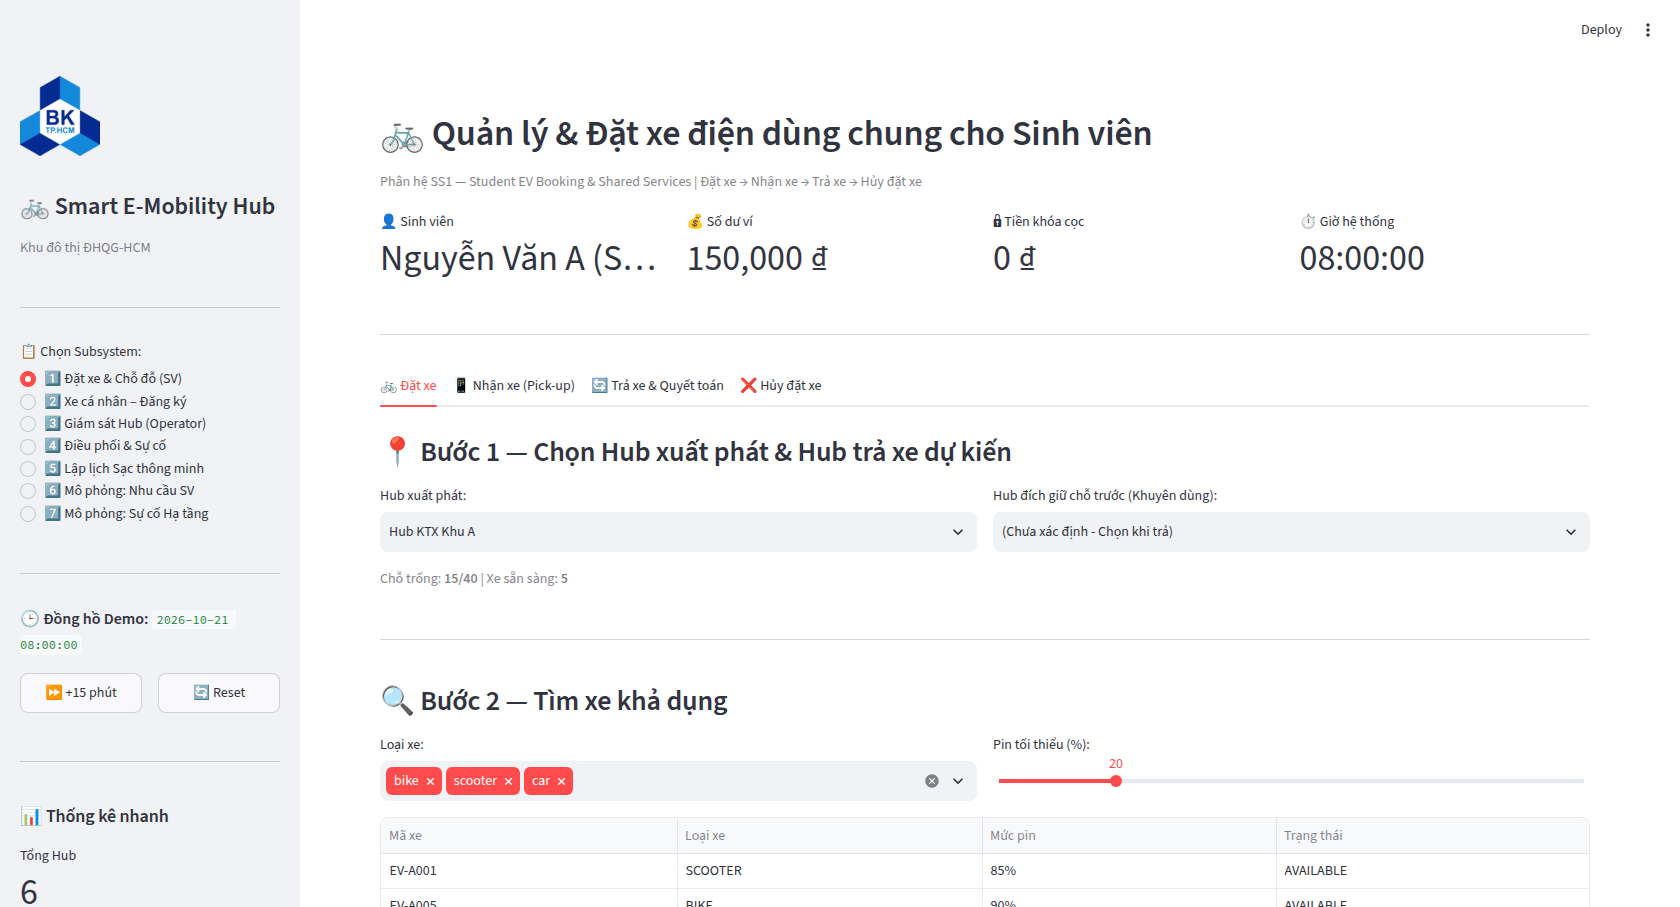
\includegraphics[width=0.92\textwidth,height=0.36\textheight,keepaspectratio]{screenshots/ss1_student_booking.png}
    \caption{Giao diện Thực tế Prototype: Đặt xe \& Quản lý Chỗ đỗ dành cho Sinh viên (Phân hệ SS1)}
    \label{fig:ui-ss1-real}
    Giao diện thực tế thể hiện sinh viên Nguyễn Văn A đang thực hiện quy trình 3 bước tại Hub KTX Khu A: chọn trạm, lọc danh sách xe khả dụng với mã màu pin trực quan, áp dụng voucher sinh viên và sẵn sàng khóa cọc 15 phút.
\end{figure}

\clearpage
\subsubsection{Phân hệ SS2: Đăng ký Phương tiện EV Cá nhân \& Quản lý Bãi đỗ (Hình \ref{fig:ui-ss2-real})}
Phân hệ SS2 (\path{src/components/personal_ev.py}) giải quyết bài toán quản lý xe điện cá nhân của sinh viên và cán bộ khi vào gửi hoặc sạc tại Hub:
\begin{itemize}[nosep]
    \item \textbf{Cấu trúc 4 Tabs quản trị phương tiện cá nhân:} Gồm \textit{Đăng ký xe mới}, \textit{Đặt chỗ \& Sạc}, \textit{Check-in}, và \textit{Check-out \& Quyết toán}; danh sách xe đã đăng ký hiển thị phía dưới.
    \item \textbf{Đăng ký phương tiện:} Biểu mẫu thu thập họ tên, biển số, loại xe, hãng xe và dung lượng pin. Hệ thống kiểm tra biển số trùng, cấp mã PEV duy nhất và lưu dữ liệu trong phiên.
    \item \textbf{Đặt chỗ trước:} Chủ xe chọn Hub, giờ đến dự kiến, nhu cầu sạc và mức pin. Cọc giữ chỗ là 50.000 VNĐ; hạn Check-in là 15 phút sau giờ đến đã đặt. Prototype giữ chỗ đỗ ngay khi xác nhận, còn cổng sạc được cấp khi Check-in theo năng lực khả dụng.
    \item \textbf{Vòng đời và quyết toán:} Check-in chuyển chỗ giữ thành xe hiện diện; Check-out hoàn cọc, giải phóng chỗ và xuất hóa đơn gộp phí đỗ, điện năng, quá giờ. QR, barie và chỉ số điện được mô phỏng; ví dùng sổ cái nội bộ.
\end{itemize}

\begin{figure}[H]
    \centering
    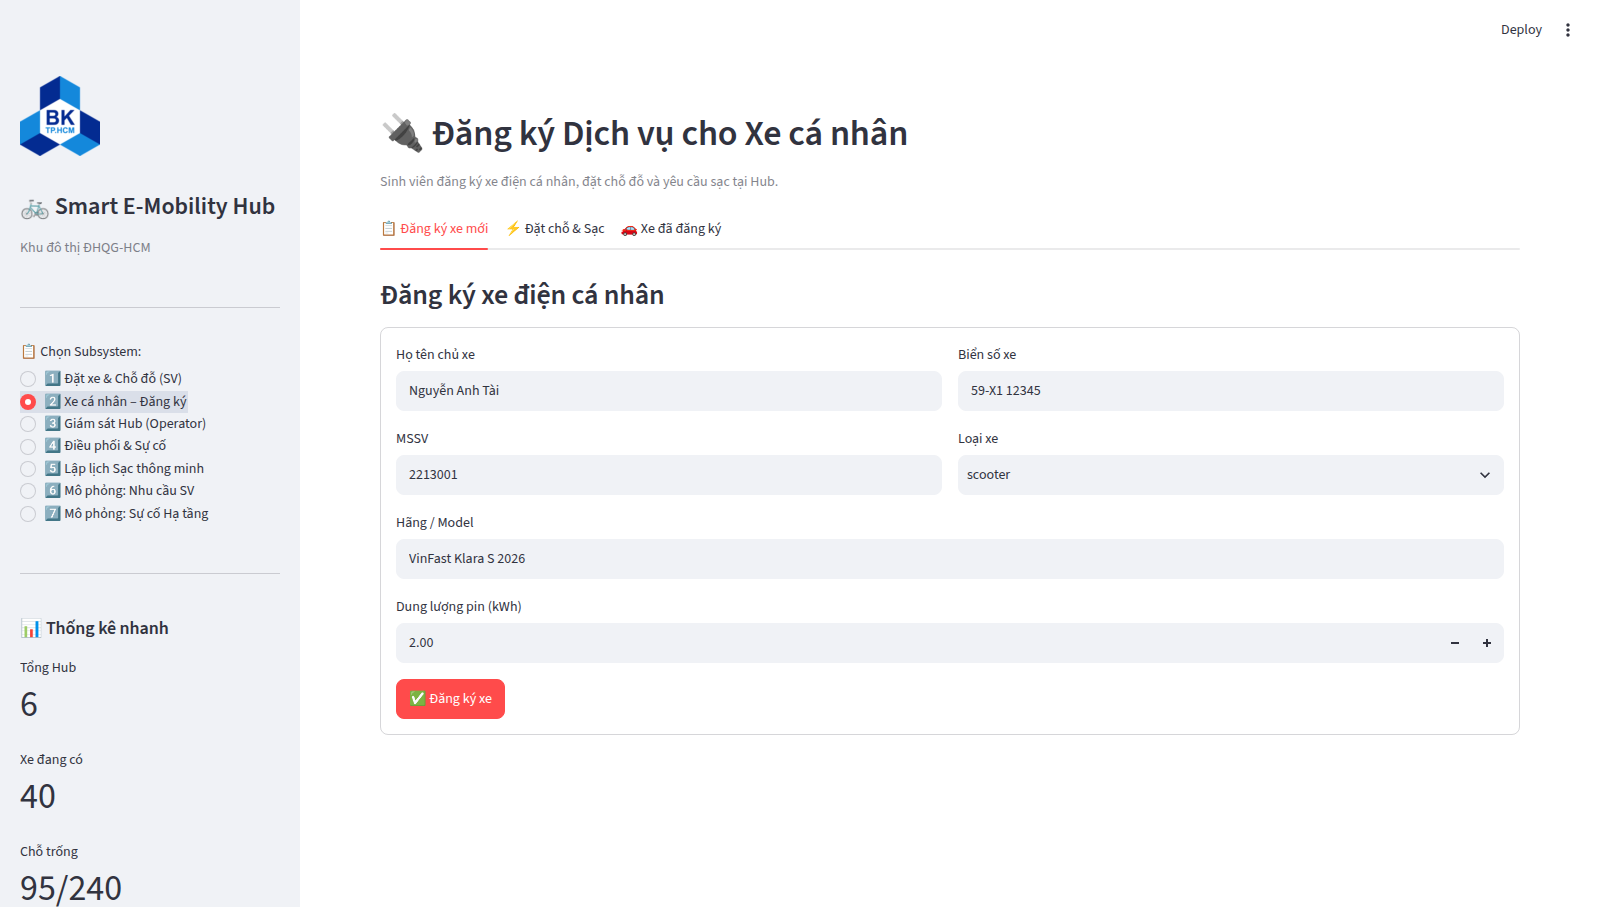
\includegraphics[width=0.92\textwidth,height=0.36\textheight,keepaspectratio]{screenshots/ss2_personal_ev.png}
    \caption{Giao diện Thực tế Prototype: Đăng ký Phương tiện EV Cá nhân \& Quản lý Bãi đỗ (Phân hệ SS2)}
    \label{fig:ui-ss2-real}
    Giao diện đặt chỗ sau khi đăng ký xe cá nhân, cho chọn giờ đến, nhu cầu sạc và hiển thị biểu phí/cọc; bốn tab hỗ trợ đầy đủ hành trình Đăng ký, Đặt chỗ, Check-in và Check-out.
\end{figure}

\clearpage
\subsection{Giao diện Thực tế Phân hệ Vận hành \& Điều phối (SS3, SS4, SS5)}
Trung tâm vận hành và điều phối mạng lưới (\texttt{hub\_monitor.py}, \texttt{dispatch\_incident.py}, \texttt{smart\_charging.py}) được chuẩn hóa cho màn hình Dashboard giám sát điều hành (Desktop/Wall-board Resolution) của Cán bộ Vận hành (Hub Operator). Thiết kế tuân thủ nghiêm ngặt nguyên lý công thái học nhận thức (\textit{Cognitive Ergonomics}) nhằm hỗ trợ phát hiện điểm nghẽn và đưa ra quyết định xử lý nhanh chóng:
\begin{itemize}[nosep]
    \item \textbf{Kiến trúc hiển thị phân tầng (Hierarchical Layout):} Cung cấp góc nhìn 3 cấp độ: Cấp độ vĩ mô toàn đô thị (Bộ 4 thẻ KPIs tổng hợp), Cấp độ trạm Hub (Mã màu cảnh báo quá tải $70\%/85\%$), và Cấp độ chi tiết thiết bị (Tình trạng từng xe và từng trụ sạc).
    \item \textbf{Phân định vai trò Operator vs Admin:} Giao diện trao quyền cho Operator thao tác trực tiếp trên dữ liệu thời gian thực: phát lệnh điều xe thừa sang thiếu, bật/tắt (Activate/Deactivate) cổng sạc phục vụ bảo dưỡng khẩn cấp, mà không cần can thiệp mức cơ sở dữ liệu.
    \item \textbf{Tối ưu hóa hàng đợi sạc đa tiêu chí:} Tự động chấm điểm ưu tiên phương tiện theo dung lượng pin xả sâu (SoC) và lịch đặt trước, tự động hóa chấm điểm dựa trên thuật toán đa mục tiêu.
\end{itemize}

Bảng \ref{tab:ui-operator-screens} dưới đây đặc tả các màn hình điều khiển nghiệp vụ phục vụ công tác giám sát, điều phối và sạc thông minh:

\begin{table}[H]
    \centering
    \small
    \renewcommand{\arraystretch}{1.2}
    \caption{Đặc tả Các Màn hình Bảng điều khiển Vận hành \& Điều phối}
    \label{tab:ui-operator-screens}
    \begin{tabularx}{\textwidth}{|l|l|X|}
        \hline
        \textbf{Mã MH} & \textbf{Tên Màn hình / Chức năng} & \textbf{Các Thành phần Giao diện \& Dữ liệu Chính} \\
        \hline
        D-01 & Dashboard Giám sát Mạng lưới (SS3) & 4 thẻ KPI đô thị, cảnh báo quá tải $>85\%$, bản đồ số 6 Hub. \\
        \hline
        D-02 & Quản lý Tài nguyên \& Thiết bị (SS3/SS7) & Bật/Tắt (Activate/Deactivate) cổng sạc, trụ xe theo thời gian thực. \\
        \hline
        D-03 & Trung tâm Điều phối Xe (SS4) & Bảng ma trận tải 6 Hub, form chuyển xe từ Hub thừa sang Hub thiếu. \\
        \hline
        D-04 & Báo cáo \& Xử lý Sự cố (SS4) & Ghi nhận hư hỏng, phân loại cấp độ (Khẩn cấp, Cao, TB), lưu nhật ký. \\
        \hline
        D-05 & Lập lịch Sạc Thông minh (SS5) & Bảng hàng đợi tính điểm ưu tiên SoC/Booking, cơ chế Overstay Fee. \\
        \hline
    \end{tabularx}
\end{table}

\clearpage
\subsubsection{Phân hệ SS3: Giám sát Mạng lưới Hub Thời gian thực (Hình \ref{fig:ui-ss3-real})}
Bảng điều khiển giám sát mạng lưới cung cấp bức tranh tổng thể về hạ tầng toàn đô thị ĐHQG-HCM:
\begin{itemize}[nosep]
    \item \textbf{Bộ 4 thẻ KPI vận hành trọng yếu:} Tổng số xe hiện hữu trên mạng lưới ($40\text{ xe}$), Tỉ lệ lấp đầy bình quân ($60.4\%$), Tổng chỗ trống khả dụng ($95/240\text{ chỗ}$), và Tổng số cổng sạc khả dụng ($25/59\text{ cổng}$).
    \item \textbf{Hộp cảnh báo quá tải tự động (Red Visual Alert):} Hệ thống giám sát tự động kích hoạt cảnh báo đỏ nổi bật khi phát hiện trạm vượt ngưỡng tải cảnh báo ($> 85\%$): \textit{"Hub KTX Khu B -- Tỉ lệ lấp đầy: 87\% $\rightarrow$ Cần điều phối!"}.
    \item \textbf{Bản đồ tương tác các trạm Hub (Streamlit map / PyDeck):} Thể hiện tọa độ địa lý thực tế của 6 Hub trung tâm trong khuôn viên ĐHQG-HCM (KTX Khu A, KTX Khu B, Nhà Khách, ĐH Bách Khoa, ĐH KHXH\&NV, ĐH CNTT) với trực quan hóa vị trí các trạm kết hợp ma trận giám sát tải theo ngưỡng quy định: $<70\%$ Bình thường (xanh), $70-85\%$ Mức cao (vàng), $>85\%$ Quá tải (đỏ).
    \item \textbf{Quản lý thiết bị thời gian thực:} Hỗ trợ Operator thao tác bật/tắt (Activate/Deactivate) các cổng sạc hoặc khóa xe phục vụ bảo trì mà không cần can thiệp mức cơ sở dữ liệu.
\end{itemize}

\begin{figure}[H]
    \centering
    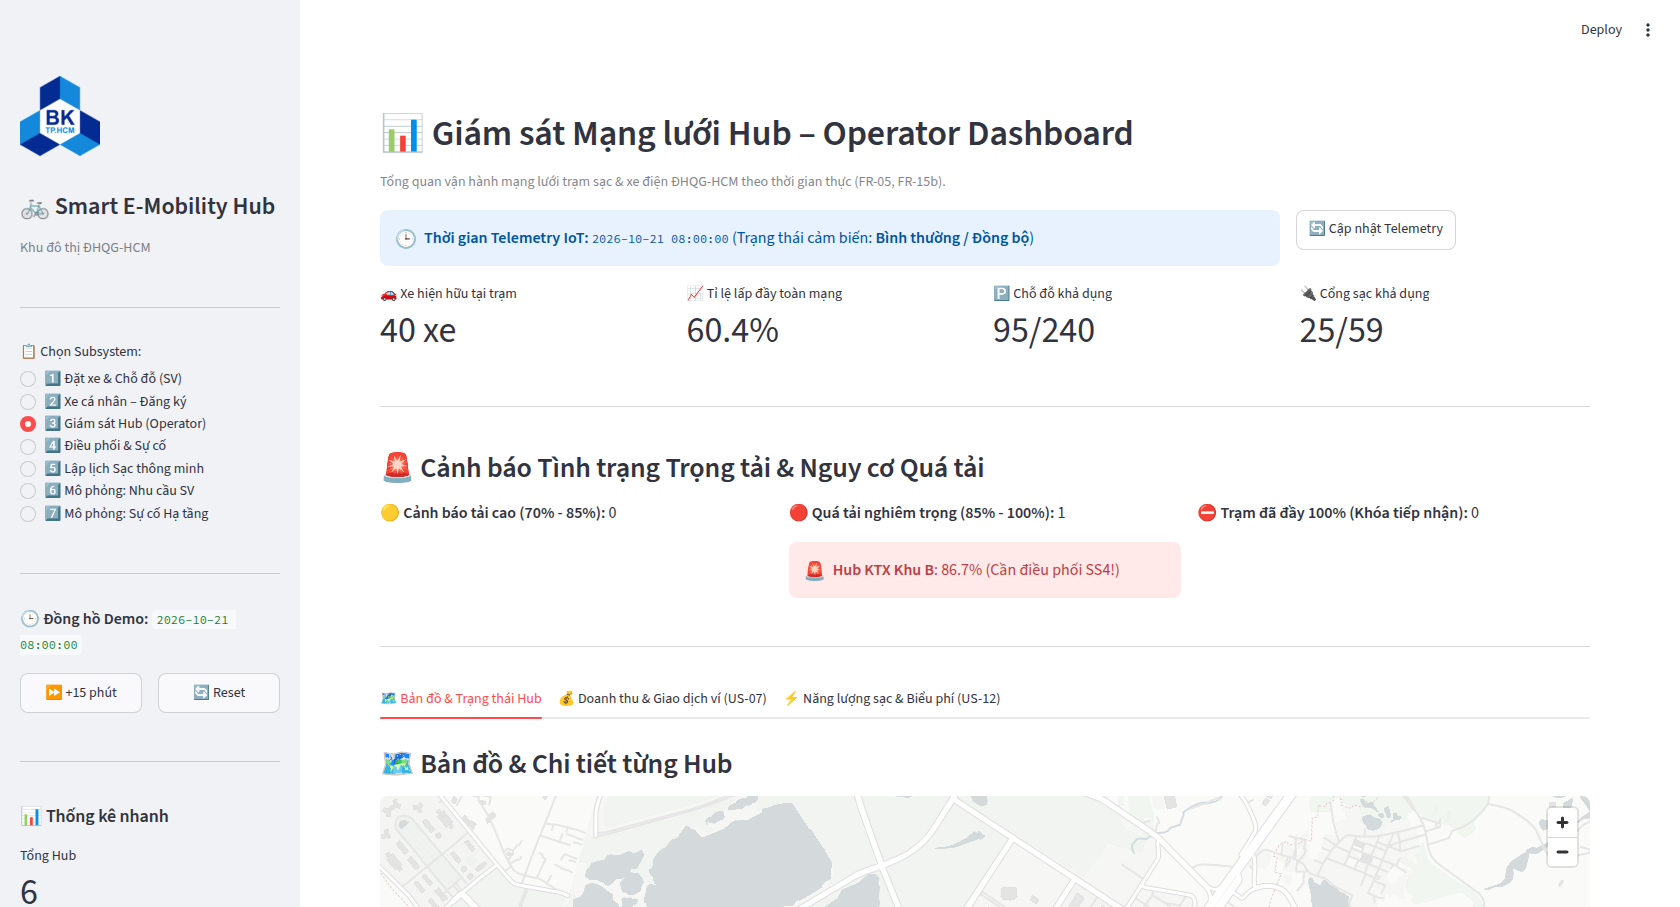
\includegraphics[width=0.92\textwidth,height=0.36\textheight,keepaspectratio]{screenshots/ss3_hub_monitor.png}
    \caption{Giao diện Thực tế Prototype: Bảng Điều khiển Giám sát Mạng lưới Hub Thời gian thực (Phân hệ SS3)}
    \label{fig:ui-ss3-real}
    Màn hình Operator Dashboard hiển thị 4 KPI vận hành cốt lõi, cảnh báo quá tải tức thời tại Hub KTX Khu B (87\%) và bản đồ GIS định vị 6 Hub trong khu đô thị ĐHQG-HCM.
\end{figure}

\clearpage
\subsubsection{Phân hệ SS4: Điều phối Cân bằng Tải \& Xử lý Sự cố Kỹ thuật (Hình \ref{fig:ui-ss4-real})}
Hỗ trợ Operator xử lý trực tiếp tình trạng mất cân đối phương tiện và sự cố kỹ thuật phát sinh:
\begin{itemize}[nosep]
    \item \textbf{Tabs chức năng nghiệp vụ:} Gồm \textit{Điều phối xe}, \textit{Báo cáo sự cố}, và \textit{Nhật ký}.
    \item \textbf{Ma trận trạng thái tải 6 Hub:} Hiển thị đầy đủ số xe, chỗ trống, tỷ lệ lấp đầy và phân loại trạng thái theo ngưỡng quy định:
    \begin{itemize}[nosep]
        \item Hub KTX Khu B: $10\text{ xe}$, $8\text{ chỗ trống}$, lấp đầy $\mathbf{86.7\%}$ $\rightarrow$ \textbf{Quá tải} (chấm đỏ, $>85\%$).
        \item Hub KTX Khu A: $8\text{ xe}$, $15\text{ chỗ trống}$, lấp đầy $\mathbf{62.5\%}$ $\rightarrow$ \textbf{Bình thường} (thuộc dải an toàn $<70\%$).
        \item Hub Trường ĐH Bách Khoa: $7\text{ xe}$, $20\text{ chỗ trống}$, lấp đầy $\mathbf{60.0\%}$ $\rightarrow$ \textbf{Bình thường} (chấm xanh).
        \item Các Hub Nhà Khách ($52\%$), ĐH KHXH\&NV ($40\%$), ĐH CNTT ($37.1\%$) đều ở trạng thái bình thường.
    \end{itemize}
    \item \textbf{Biểu mẫu phát lệnh điều phối xe chuẩn hóa:} Cho phép chọn Hub nguồn thừa xe (\textbf{Hub KTX Khu B}), Hub đích còn nhiều chỗ trống (\textbf{Hub Trường ĐH Bách Khoa}), chọn các xe cụ thể cần điều chuyển (\texttt{EV-B001} - scooter SoC $60\%$, \texttt{EV-B003} - scooter SoC $12\%$) và nhập lý do điều phối rõ ràng.
    \item \textbf{Nhật ký \& Theo dõi sự cố:} Tiếp nhận thông tin báo hỏng phương tiện hoặc chập cháy cổng sạc, phân loại mức độ nghiêm trọng và lưu vết vào hệ thống kiểm toán vận hành.
\end{itemize}

\begin{figure}[H]
    \centering
    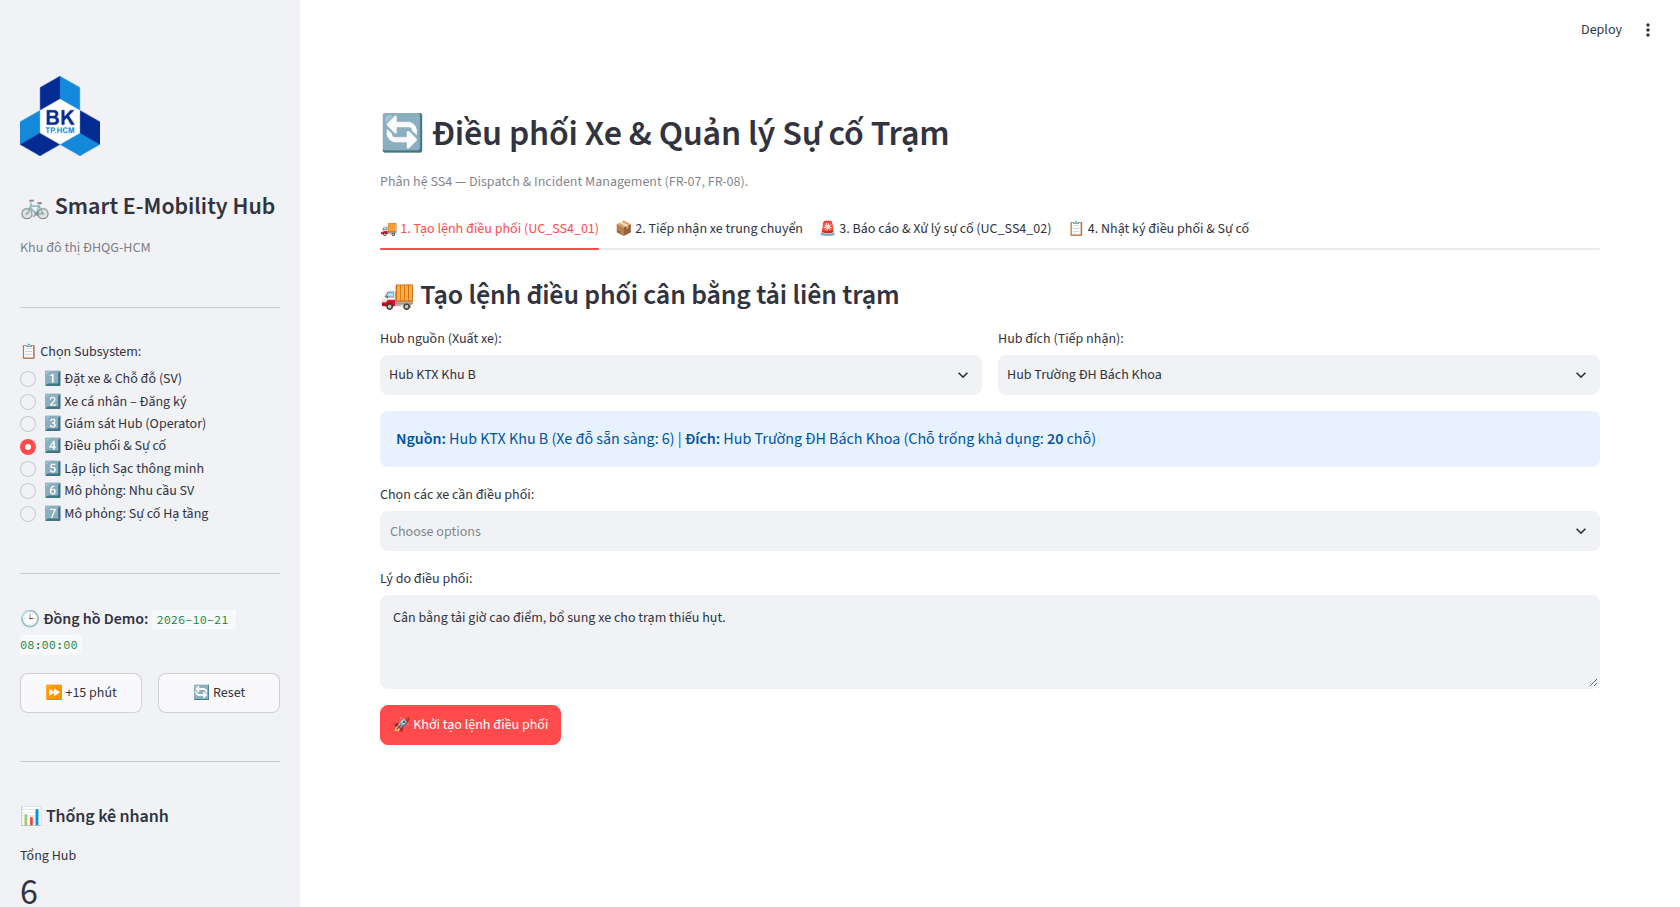
\includegraphics[width=0.92\textwidth,height=0.36\textheight,keepaspectratio]{screenshots/ss4_dispatch_incident.png}
    \caption{Giao diện Thực tế Prototype: Điều phối Cân bằng Tải \& Xử lý Sự cố Kỹ thuật (Phân hệ SS4)}
    \label{fig:ui-ss4-real}
    Ma trận trực quan tình trạng tải của 6 Hub trong mạng lưới và biểu mẫu phát lệnh điều phối phương tiện từ Hub KTX Khu B (đang quá tải 86.7\%) sang Hub ĐH Bách Khoa (còn 20 chỗ trống).
\end{figure}

\clearpage
\subsubsection{Phân hệ SS5: Lập lịch Sạc Thông minh \& Quản lý Hàng đợi (Hình \ref{fig:ui-ss5-real})}
Ứng dụng thuật toán tối ưu hóa đa mục tiêu nhằm phân bổ hợp lý công suất trạm sạc cho các phương tiện:
\begin{itemize}[nosep]
    \item \textbf{Bộ chỉ số trạng thái hàng đợi sạc:} Tổng số xe trong hàng đợi ($8\text{ xe}$), Số lượng xe đang sạc ($0\text{ xe}$), Số lượng xe pin nguy hiểm $\text{SoC} < 20\%$ ($1\text{ xe}$), và Số lượng xe gắn lịch đặt trước của sinh viên ($0\text{ xe}$).
    \item \textbf{Hàng đợi sạc sắp xếp tự động theo điểm ưu tiên:} Thuật toán chấm điểm dựa trên công thức đa tiêu chí hiện thực tại \path{src/core/scheduler.py}:
    \begin{equation}
        \text{Score} = (100 - \text{SoC}) \times 0.5 + 100 \times \mathbb{I}(\text{SoC} < 20\%) + 60 \times \mathbb{I}(\text{HasBooking}) + 30 \times \mathbb{I}(\text{SoC} < 50\%)
    \end{equation}
    trong đó $\mathbb{I}(\cdot)$ là hàm chỉ thị nhận giá trị $1$ nếu điều kiện thỏa mãn và $0$ nếu không. Điểm số phản ánh chính xác mức độ khẩn cấp:
    \begin{itemize}[nosep]
        \item $1\text{ xe}$ có mức pin nguy hiểm ($\text{SoC} < 20\%$) được xếp ưu tiên hàng đầu và tô màu hồng/đỏ nhạt nổi bật: Top 1 là \texttt{EV-B005} ($\text{SoC} = 18\%$, không booking): $\text{Score} = (100 - 18) \times 0.5 + 100 + 0 + 30 = 41.0 + 130 = \mathbf{171.0}$.
        \item Các xe có mức pin an toàn hơn ($\text{SoC} \ge 20\%$) được xếp theo sau và giữ màu nền trắng. Cụ thể: Top 2 là \texttt{EV-D002} ($\text{SoC} = 20\%$, $\text{Score} = \mathbf{70.0}$); Top 3 là \texttt{EV-E003} ($\text{SoC} = 22\%$, $\text{Score} = \mathbf{69.0}$); tiếp đến \texttt{EV-B002} ($25\%$, $\text{Score} = \mathbf{67.5}$); \texttt{EV-D007} ($30\%$, $\text{Score} = \mathbf{65.0}$); \texttt{EV-F002} ($35\%$, $\text{Score} = \mathbf{62.5}$); \texttt{EV-A002} ($42\%$, $\text{Score} = \mathbf{59.0}$); và cuối cùng là \texttt{EV-A007} ($55\%$, $\text{Score} = \mathbf{22.5}$).
    \end{itemize}
    \item \textbf{Cơ chế phạt quá hạn cổng sạc (Overstay Fee):} Khi sạc đạt ngưỡng $100\%$, đồng hồ đếm ngược 15 phút ân hạn kích hoạt. Sau thời gian này, hệ thống tự động áp phí chiếm dụng cổng nhằm giải phóng chỗ cho xe tiếp theo trong hàng đợi.
\end{itemize}

\begin{figure}[H]
    \centering
    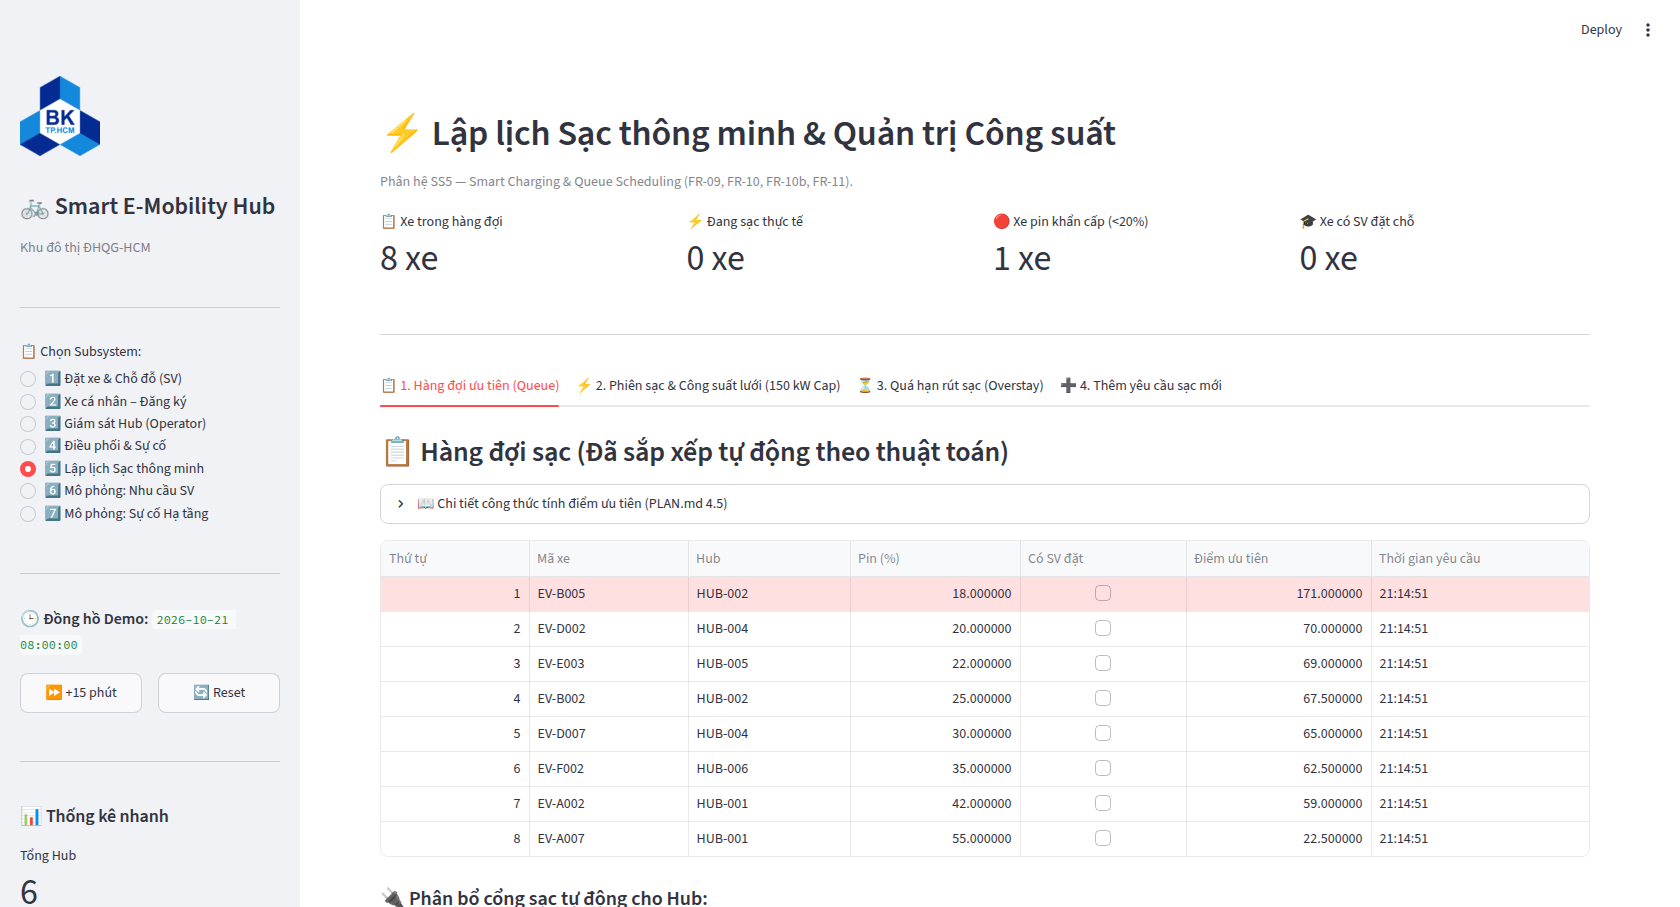
\includegraphics[width=0.92\textwidth,height=0.36\textheight,keepaspectratio]{screenshots/ss5_smart_charging.png}
    \caption{Giao diện Thực tế Prototype: Lập lịch Sạc Thông minh \& Quản lý Hàng đợi (Phân hệ SS5)}
    \label{fig:ui-ss5-real}
    Bảng hàng đợi sạc thông minh được tự động sắp xếp theo điểm ưu tiên đa mục tiêu, làm nổi bật phương tiện có mức pin nguy hiểm (<20\%) bằng mã màu hồng/đỏ để ưu tiên cấp nguồn sạc trước.
\end{figure}

\clearpage
\subsection{Giao diện Thực tế Phân hệ Mô phỏng What-if (SS6 \& SS7)}
Công cụ phân tích và giả lập kịch bản chuyên sâu (\path{sim_demand.py} và \path{sim_infrastructure.py}) phục vụ công tác dự báo, đánh giá rủi ro và chuẩn bị phương án ứng phó vận hành:

\begin{table}[H]
    \centering
    \small
    \renewcommand{\arraystretch}{1.2}
    \caption{Đặc tả Màn hình Cấu hình \& Báo cáo Mô phỏng What-if}
    \label{tab:ui-whatif-screens}
    \begin{tabularx}{\textwidth}{|l|l|X|}
        \hline
        \textbf{Mã MH} & \textbf{Tên Màn hình / Chức năng} & \textbf{Các Thành phần Giao diện \& Dữ liệu Chính} \\
        \hline
        W-01 & Cấu hình Kịch bản Metro Surge (SS6) & Thanh trượt Surge Multiplier ($1\times - 5\times$), số giờ mô phỏng. \\
        \hline
        W-02 & Biểu đồ Tác động Nhu cầu (SS6) & Biểu đồ Plotly 2 trục tung: lượng SV đến và hàng đợi tích lũy. \\
        \hline
        W-03 & Giả lập Sự cố Hạ tầng Port Failure (SS7) & Bảng chọn Hub bị sự cố, số cổng hỏng, nút kích hoạt giả lập. \\
        \hline
        W-04 & Đề xuất Điều phối \& Rerouting (SS7) & Quét Hub lân cận, bảng đề xuất chuyển trạm, nút áp dụng 1-chạm. \\
        \hline
    \end{tabularx}
\end{table}

\clearpage
\subsubsection{Phân hệ SS6: Mô phỏng Nhu cầu Đột biến Metro Surge (Hình \ref{fig:ui-ss6-real})}
Giúp nhà vận hành thử nghiệm các kịch bản gia tăng hành khách đột ngột khi tuyến Metro số 1 (Bến Thành -- Suối Tiên) xả khách tại ga ĐHQG-HCM:
\begin{itemize}[nosep]
    \item \textbf{Cấu hình tham số mô phỏng trực quan:} Cho phép tùy chỉnh tỉ lệ sinh viên đến cơ bản ($15\text{ SV/giờ}$), thanh trượt hệ số tăng đột biến (Surge Multiplier $1.00\times - 5.00\times$), và số giờ mô phỏng ($12\text{ giờ}$).
    \item \textbf{Biểu đồ phân tích Plotly tương tác 2 trục tung:}
    \begin{itemize}[nosep]
        \item Cột màu lam (trục tung trái): Biểu diễn số lượng sinh viên đổ về Hub theo từng mốc thời gian trong ngày (đạt đỉnh gần $40\text{ người/giờ}$ vào các khung giờ 08:00 sáng và 17:00 chiều).
        \item Đường đỏ cam (trục tung phải): Thể hiện độ dài hàng đợi tích lũy dồn ứ tăng dần từ sáng sớm đến cuối buổi chiều (vượt mốc $150\text{ người}$ nếu không có biện pháp điều phối xe kịp thời).
    \end{itemize}
    \item \textbf{Ứng dụng hỗ trợ ra quyết định:} Giúp người vận hành dự báo trước chính xác số lượng phương tiện cần điều động bổ sung về trạm ga Metro trước các khung giờ cao điểm.
\end{itemize}

\begin{figure}[H]
    \centering
    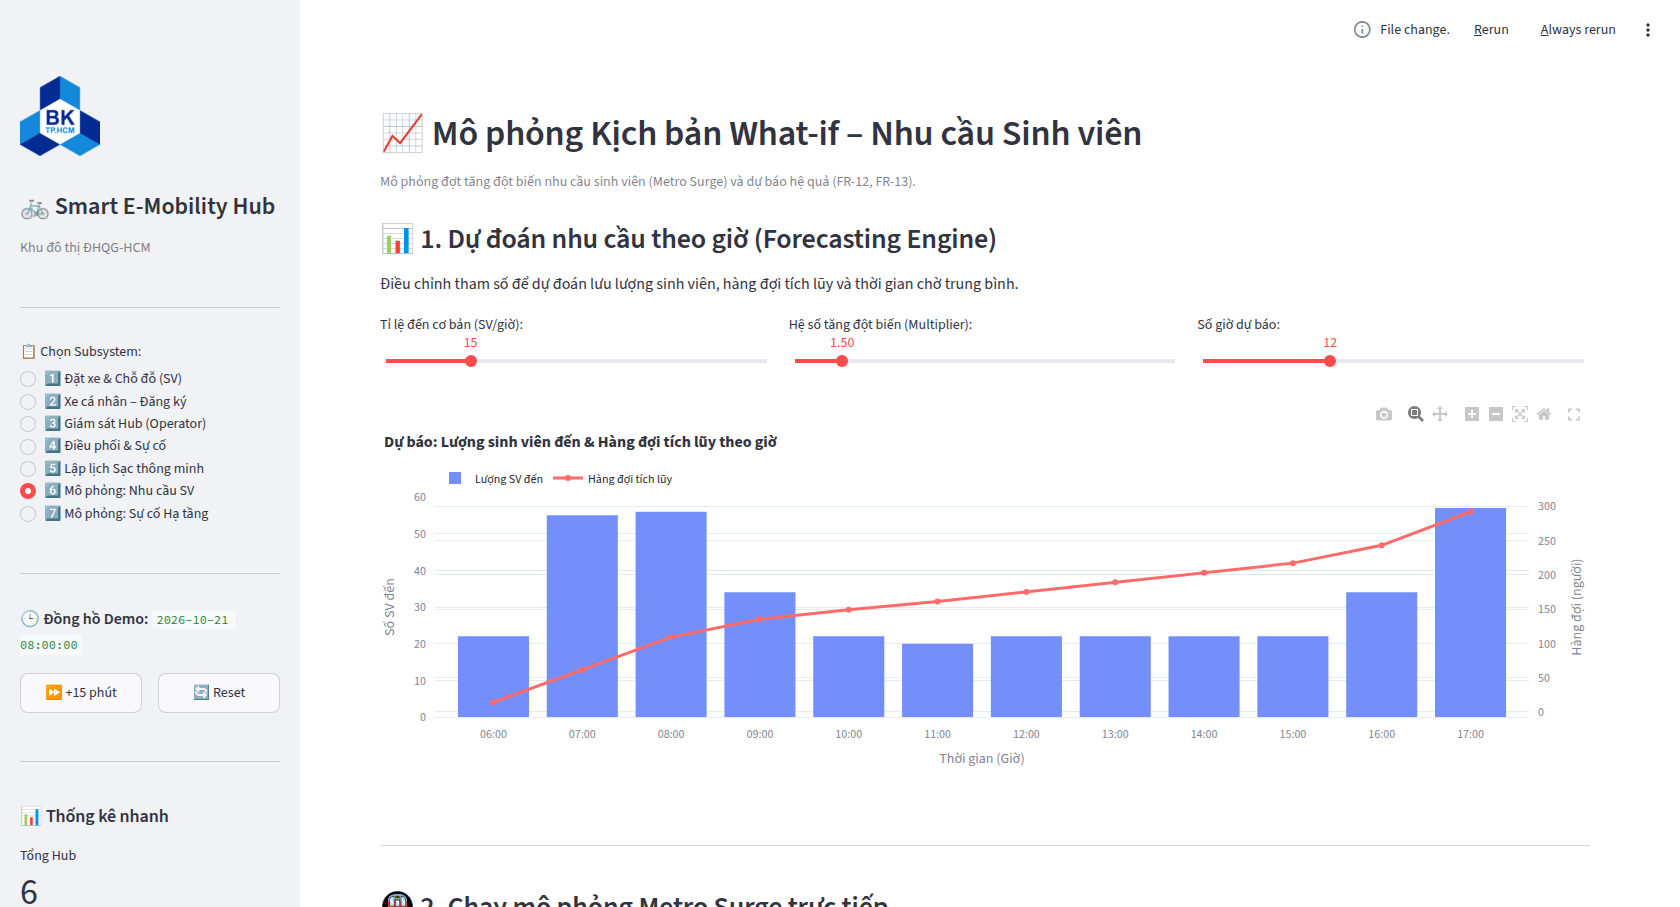
\includegraphics[width=0.92\textwidth,height=0.36\textheight,keepaspectratio]{screenshots/ss6_sim_demand.png}
    \caption{Giao diện Thực tế Prototype: Bảng Điều khiển Mô phỏng Nhu cầu Metro Surge (Phân hệ SS6)}
    \label{fig:ui-ss6-real}
    Biểu đồ trực quan hóa dự báo nhu cầu đi lại theo giờ với 2 trục tung (lượng sinh viên đến vs hàng đợi tích lũy dồn ứ), phục vụ hoạch định nguồn lực trước các đợt tăng tải Metro.
\end{figure}

\clearpage
\subsubsection{Phân hệ SS7: Mô phỏng Sự cố Hạ tầng \& Gợi ý Điều hướng 1-chạm (Hình \ref{fig:ui-ss7-real})}
Giả lập sự cố mất điện trạm sạc hoặc hỏng thiết bị và tự động kích hoạt kịch bản điều hướng phương tiện thông minh:
\begin{itemize}[nosep]
    \item \textbf{Kịch bản giả lập Port Failure:} Chọn Hub Trường ĐH Bách Khoa và mô phỏng hỏng 4 cổng. Kết quả phân biệt cổng rảnh và cổng đang sạc, không giảm số cổng khả dụng bằng phép trừ đơn giản khi cổng hỏng đang được sử dụng.
    \item \textbf{Nhật ký sự kiện:} Preview ghi thời điểm chạy, xe bị gián đoạn và số cổng còn khả dụng; các xe EV-D002 và EV-D007 bị ảnh hưởng chuyển sang trạng thái WAITING trong dữ liệu xem trước.
    \item \textbf{Gợi ý trạm thay thế:} Từ dữ liệu preview, hệ thống sắp xếp theo khoảng cách và hiển thị tối đa hai Hub còn cổng sạc; ví dụ Hub KTX Khu A và Hub Nhà Khách ĐHQG trong ảnh minh họa.
    \item \textbf{Áp dụng và điều hướng:} Nút áp dụng tại SS7 chỉ ghi nhận sự cố mô phỏng vào trạng thái vận hành và từ chối preview đã cũ. Khi trả xe tại SS1 gặp Hub đầy, sinh viên chọn một trong hai Hub gợi ý để chuyển giữ chỗ bằng một nút bấm; hệ thống hoàn giữ chỗ cũ, giữ chỗ mới và cộng thêm 15 phút miễn phí một lần.
\end{itemize}

\begin{figure}[H]
    \centering
    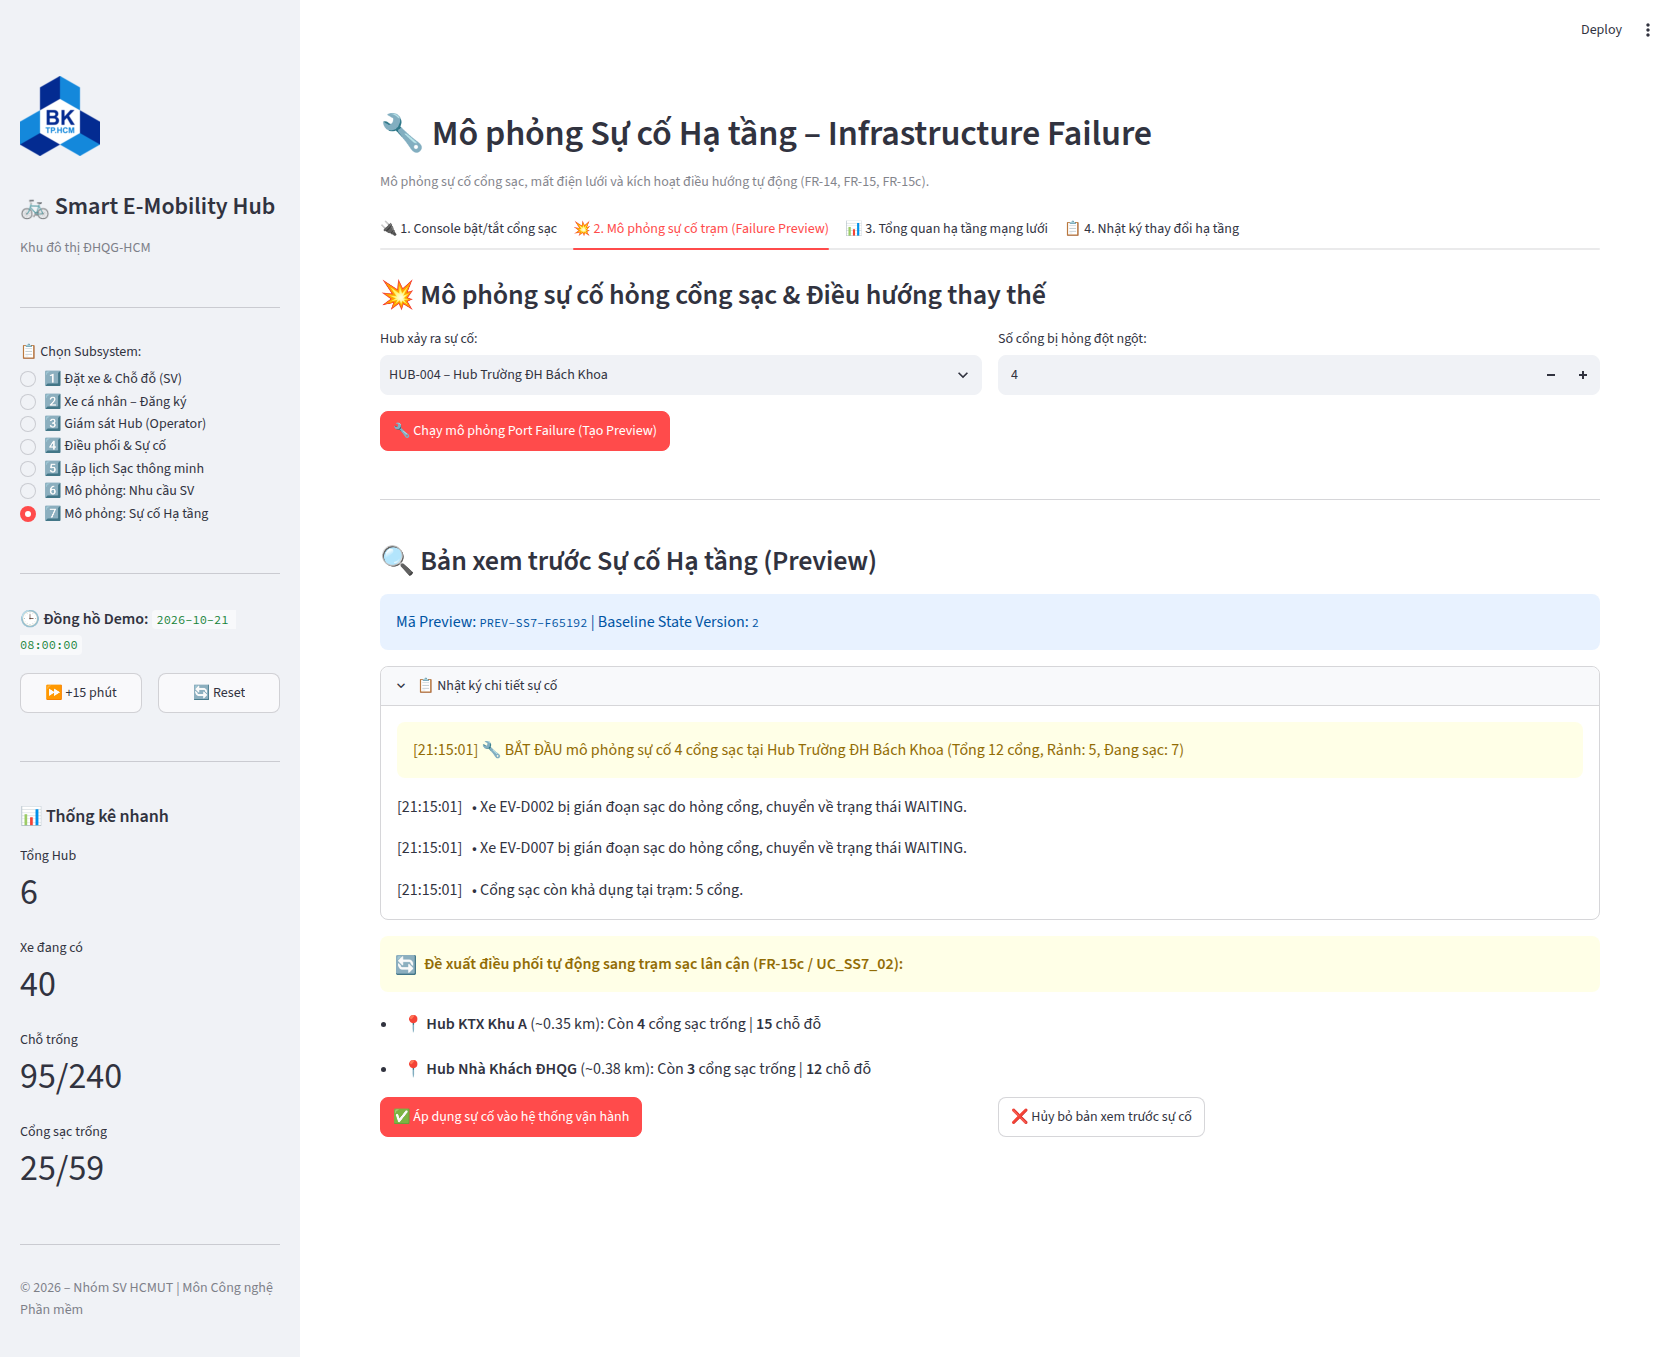
\includegraphics[width=0.92\textwidth,height=0.36\textheight,keepaspectratio]{screenshots/ss7_sim_infrastructure.png}
    \caption{Giao diện Thực tế Prototype: Mô phỏng Sự cố Hạ tầng \& Gợi ý Điều hướng 1-chạm (Phân hệ SS7)}
    \label{fig:ui-ss7-real}
    Bảng điều khiển tạo preview sự cố cổng sạc tại Hub ĐH Bách Khoa, ghi nhật ký và đề xuất hai Hub còn cổng sạc lân cận; nút áp dụng chỉ cập nhật khi phiên bản dữ liệu còn hợp lệ.
\end{figure}

\clearpage
% ============================================================
%       MỤC 2: SƠ ĐỒ TUẦN TỰ - SEQUENCE DIAGRAMS (INDIVIDUAL WORK)
% ============================================================
\section{Sơ đồ Tuần tự -- Sequence Diagrams (Individual Work)}

Mục này trình bày chi tiết \textbf{17 Sơ đồ Tuần tự (Sequence Diagrams)} tương ứng với 17 kịch bản Use-Case của hệ thống Smart E-Mobility Hub, được phân công độc lập cho từng thành viên. Mỗi sơ đồ làm rõ các luồng trao đổi thông điệp, kiểm tra điều kiện rẽ nhánh (\texttt{alt}), vòng lặp (\texttt{loop}) và các ngoại lệ kỹ thuật (\texttt{break}/\texttt{critical}).

\subsection*{Nguyên tắc Mô hình hóa Tương tác \& Phân định Vai trò Hệ thống}
Để đảm bảo tính chuẩn xác theo chuẩn UML 2.5 và phản hồi chuyên môn từ Giảng viên, toàn bộ các sơ đồ tuần tự tuân thủ nghiêm ngặt các nguyên lý:
\begin{itemize}[nosep]
    \item \textbf{Phân định minh bạch Operator và Admin:} Tác nhân \textit{Nhân viên Vận hành (Operator)} trực tiếp tương tác trên dữ liệu thời gian thực (giám sát, kích hoạt/tắt thiết bị, phát lệnh điều chuyển xe). Trong khi đó, \textit{Quản trị viên (Admin)} chỉ đảm nhiệm phân quyền tài khoản (RBAC), cấu hình thông số ban đầu và can thiệp hỗ trợ khẩn cấp.
    \item \textbf{Xử lý Yêu cầu Phi tương tác (Non-interactive FRs):} Các tiến trình tự động chạy ngầm (lập lịch sạc tối ưu theo SoC, quét kiểm tra quá hạn giữ chỗ 15 phút, đồng bộ dữ liệu cảm biến IoT) được kích hoạt bởi chu kỳ thời gian (Timer/Cron) hoặc sự kiện bất đồng bộ, được biểu diễn qua Lifeline của các thành phần nội tại hệ thống (\texttt{:SchedulerService}, \texttt{:ChargingOptimizerEngine}), tuyệt đối không mô hình hóa bộ lập lịch ngầm thành một Actor con người bên ngoài.
\end{itemize}

\begin{table}[H]
    \centering
    \small
    \renewcommand{\arraystretch}{1.25}
    \caption{Ma trận Phân công Thực hiện 17 Sequence Diagrams}
    \label{tab:seq-assignment}
    \begin{tabularx}{\textwidth}{|c|c|X|l|c|}
        \hline
        \textbf{STT} & \textbf{Mã UC} & \textbf{Tên Use-Case} & \textbf{Thành viên phụ trách} & \textbf{Trạng thái} \\
        \hline
        1 & UC\_SS1\_01 & Đặt giữ chỗ \& Quét QR/PIN nhận xe & Nguyễn Thành Đạt & Hoàn thành \\
        2 & UC\_SS1\_02 & Trả xe 1-chiều \& Quyết toán ví điện tử & Nguyễn Thành Đạt & Hoàn thành \\
        3 & UC\_SS1\_03 & Hủy đặt xe \& Hoàn cọc / Phạt No-show & Nguyễn Thành Đạt & Hoàn thành \\
        \hline
        4 & UC\_SS2\_01 & Đăng ký xe EV cá nhân & Nguyễn Anh Tài & Hoàn thành \\
        5 & UC\_SS2\_02 & Đặt chỗ đỗ và nhu cầu sạc xe EV cá nhân & Nguyễn Anh Tài & Hoàn thành \\
        6 & UC\_SS2\_03 & Check-in xe EV cá nhân tại Hub & Nguyễn Anh Tài & Hoàn thành \\
        7 & UC\_SS2\_04 & Check-out và thanh toán dịch vụ xe cá nhân & Nguyễn Anh Tài & Hoàn thành \\
        \hline
        8 & UC\_SS3\_01 & Giám sát trạng thái Hub theo thời gian thực & Phạm Tiến Đạt & Hoàn thành \\
        9 & UC\_SS3\_02 & Cảnh báo quá tải \& Đề xuất điều phối & Phạm Tiến Đạt & Hoàn thành \\
        \hline
        10 & UC\_SS4\_01 & Lập lệnh điều phối phương tiện giữa các Hub & Đặng Hoàng Quý Nhân & Hoàn thành \\
        11 & UC\_SS4\_02 & Báo cáo \& Xử lý sự cố kỹ thuật phương tiện & Đặng Hoàng Quý Nhân & Hoàn thành \\
        \hline
        12 & UC\_SS5\_01 & Lập lịch ưu tiên sạc tự động & Dương Đăng Khoa & Hoàn thành \\
        13 & UC\_SS5\_02 & Giám sát hàng đợi sạc \& Phí chiếm dụng & Dương Đăng Khoa & Hoàn thành \\
        \hline
        14 & UC\_SS6\_01 & Mô phỏng đợt tăng đột biến hành khách Metro & Hoàng Văn Tấn & Hoàn thành \\
        15 & UC\_SS6\_02 & Dự báo nhu cầu theo giờ \& Phân tích hàng đợi & Hoàng Văn Tấn & Hoàn thành \\
        \hline
        16 & UC\_SS7\_01 & Mô phỏng sự cố mất điện / lỗi cổng sạc & Nguyễn Trung Nguyên & Hoàn thành \\
        17 & UC\_SS7\_02 & Tự động phát cảnh báo \& Gợi ý điều hướng 1-chạm & Nguyễn Trung Nguyên & Hoàn thành \\
        \hline
    \end{tabularx}
\end{table}

% ------------------------------------------------------------
% 2.1 SS1 - Nguyễn Thành Đạt
% ------------------------------------------------------------
\subsection{Phân hệ SS1: Đặt \& Quản lý Xe dùng chung (Nguyễn Thành Đạt)}

\subsubsection{UC\_SS1\_01: Đặt giữ chỗ \& Quét QR/PIN nhận xe}
\paragraph{Mô tả nghiệp vụ:} Sinh viên chọn Hub, chọn xe điện, thực hiện khóa cọc 50.000 VNĐ trong ví VNU-Pay. Hệ thống sinh mã OTP/QR có hiệu lực 15 phút. Tại trạm Hub, sinh viên quét QR mở khóa xe, chuyển trạng thái xe sang \texttt{IN\_USE}.

\begin{figure}[H]
    \centering
    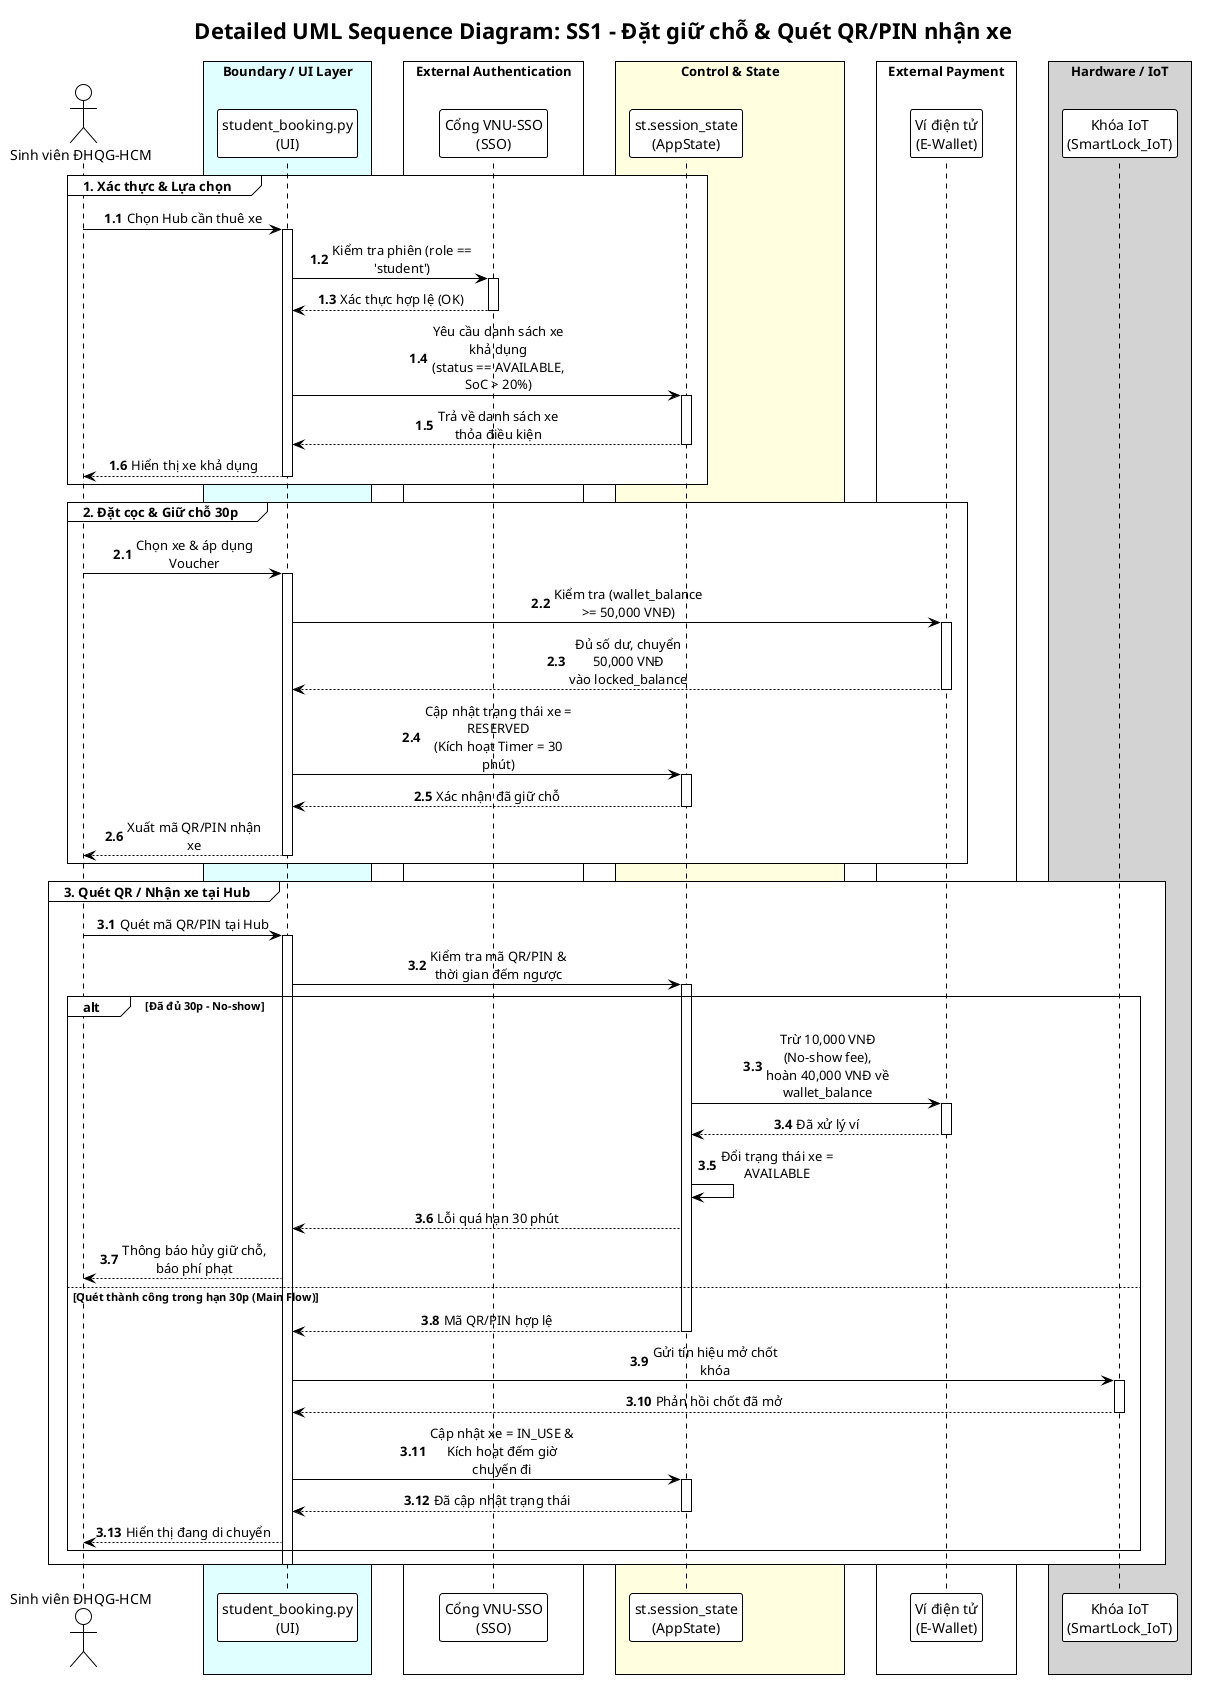
\includegraphics[width=0.88\textwidth,height=0.68\textheight,keepaspectratio]{Use-case detail-scenario/SS1/Sequence diagrams/UC_SS1_01_NguyenThanhDat_sequence.png}
    \caption{Sơ đồ Tuần tự Chi tiết -- UC\_SS1\_01 (Đặt xe \& Quét nhận xe)}
    \label{fig:seq-ss1-01}
\end{figure}

\begin{table}[H]
    \centering
    \small
    \renewcommand{\arraystretch}{1.25}
    \caption{Đặc tả Các Thông điệp Tương tác (Message Exchange Table) -- UC\_SS1\_01}
    \label{tab:msg-ss1-01}
    \begin{tabularx}{\textwidth}{|c|>{\raggedright\arraybackslash}p{2.6cm}|>{\raggedright\arraybackslash}p{2.6cm}|>{\raggedright\arraybackslash}X|}
        \hline
        \textbf{Nhóm / Bước} & \textbf{Đối tượng Gửi} & \textbf{Đối tượng Nhận} & \textbf{Tên thông điệp / Dữ liệu trao đổi} \\
        \hline
        \multicolumn{4}{|l|}{\textbf{Nhóm 1: Xác thực VNU-SSO \& Lựa chọn phương tiện}} \\
        \hline
        1.1 & Sinh viên & UI & Chọn Hub cần thuê xe \\
        1.2 & UI & Cổng VNU-SSO & Kiểm tra thông tin phiên đăng nhập (\texttt{role == 'student'}) \\
        1.3 & Cổng VNU-SSO & UI & Phản hồi xác thực hợp lệ (OK) \\
        1.4 & UI & st.session\_state & Yêu cầu danh sách xe khả dụng (\texttt{status == AVAILABLE}, $\text{SoC} > 20\%$) \\
        1.5 & st.session\_state & UI & Trả về danh sách xe thỏa điều kiện \\
        1.6 & UI & Sinh viên & Hiển thị thẻ xe khả dụng trên giao diện \\
        \hline
        \multicolumn{4}{|l|}{\textbf{Nhóm 2: Đặt cọc ví điện tử \& Giữ chỗ 15 phút}} \\
        \hline
        2.1 & Sinh viên & UI & Chọn xe cụ thể \& áp dụng mã ưu đãi (Voucher) \\
        2.2 & UI & Ví điện tử & Kiểm tra số dư khả dụng (\texttt{wallet\_balance} $\ge 50.000\text{ VNĐ}$) \\
        2.3 & Ví điện tử & UI & Đủ số dư, khóa $50.000\text{ VNĐ}$ sang \texttt{locked\_balance} \\
        2.4 & UI & st.session\_state & Cập nhật xe $\rightarrow$ \texttt{RESERVED}, kích hoạt Timer 15 phút \\
        2.5 & st.session\_state & UI & Xác nhận đã giữ chỗ thành công \\
        2.6 & UI & Sinh viên & Xuất mã QR/PIN 4 số nhận xe kèm đồng hồ đếm ngược \\
        \hline
        \multicolumn{4}{|l|}{\textbf{Nhóm 3: Quét QR/PIN nhận xe tại Hub hoặc Xử lý No-show}} \\
        \hline
        3.1 & Sinh viên & UI & Quét QR code hoặc nhập mã PIN 4 số tại Hub \\
        3.2 & UI & st.session\_state & Kiểm tra mã QR/PIN \& thời gian đếm ngược \\
        3.3a (No-show) & st.session\_state & Ví điện tử & Quá 15p: trừ phạt $10.000\text{ VNĐ}$, hoàn $40.000\text{ VNĐ}$ về ví \\
        3.4a (No-show) & st.session\_state & UI & Xe $\rightarrow$ \texttt{AVAILABLE}; UI thông báo quá hạn \& phí phạt \\
        3.3b (Main) & st.session\_state & UI & Mã QR/PIN hợp lệ (trong hạn 15 phút) \\
        3.4b (Main) & UI & Khóa IoT & Gửi tín hiệu mở chốt cơ điện (\texttt{unlock()}) \\
        3.5b (Main) & Khóa IoT & UI & Phản hồi chốt khóa vật lý đã mở \\
        3.6b (Main) & UI & st.session\_state & Đổi xe $\rightarrow$ \texttt{IN\_USE}, bắt đầu tính giờ chuyến đi \\
        3.7b (Main) & UI & Sinh viên & Hiển thị màn hình 'Đang di chuyển' \\
        \hline
    \end{tabularx}
\end{table}

\clearpage
\subsubsection{UC\_SS1\_02: Trả xe 1-chiều \& Quyết toán ví điện tử}
\paragraph{Mô tả nghiệp vụ:} Sinh viên đưa xe vào chốt khóa tại Hub bất kỳ. Tín hiệu cảm biến IoT (mô phỏng) xác thực vị trí chốt, đọc dung lượng pin hiện tại, tính cước thuê xe thực tế, hoàn lại phần cọc dư vào ví và xuất hóa đơn điện tử e-Invoice.
\begin{figure}[H]
    \centering
    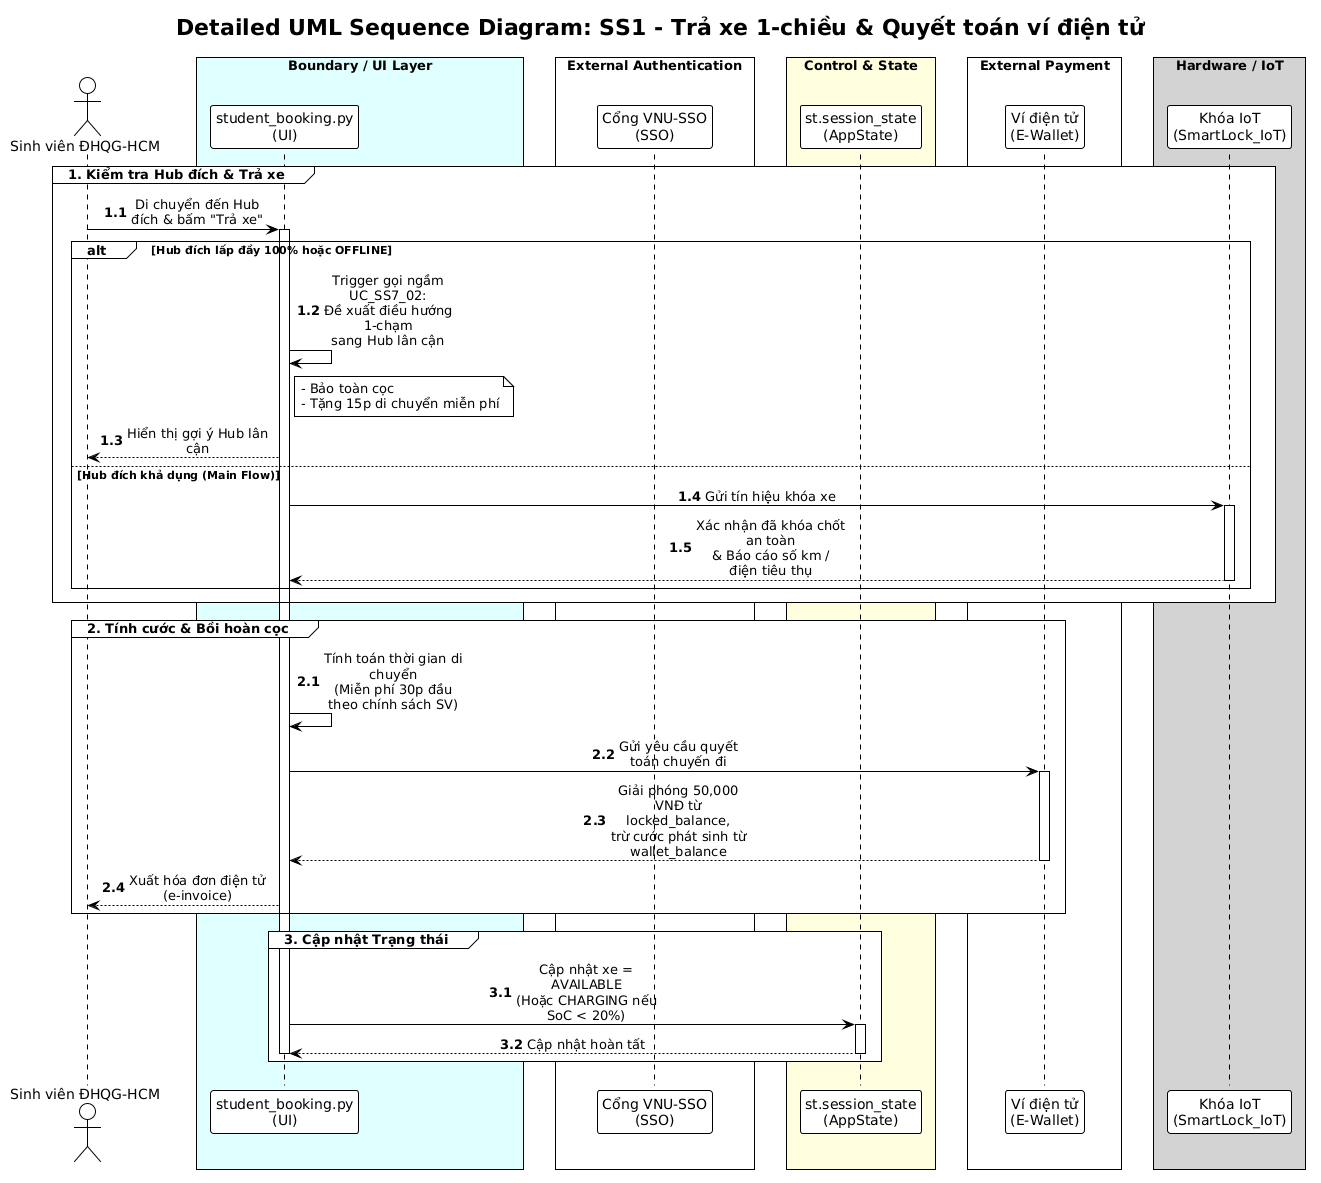
\includegraphics[width=0.88\textwidth,height=0.62\textheight,keepaspectratio]{Use-case detail-scenario/SS1/Sequence diagrams/UC_SS1_02_NguyenThanhDat_sequence.png}
    \caption{Sơ đồ Tuần tự Chi tiết -- UC\_SS1\_02 (Trả xe 1-chiều \& Quyết toán ví)}
    \label{fig:seq-ss1-02}
\end{figure}

\clearpage
\subsubsection{UC\_SS1\_03: Hủy đặt xe \& Hoàn cọc / Phạt No-show}
\paragraph{Mô tả nghiệp vụ:} Khi sinh viên chủ động hủy đặt chỗ trong thời hạn 15 phút, hệ thống tự động giải phóng xe về trạng thái \texttt{AVAILABLE} và hoàn $100\%$ tiền cọc ($50.000\text{ VNĐ}$) về ví điện tử. Trường hợp quá 15 phút mà sinh viên không đến nhận xe (No-show), hệ thống tự động hủy lệnh, áp dụng phí phạt giữ chỗ $10.000\text{ VNĐ}$ và hoàn trả $40.000\text{ VNĐ}$ còn lại về ví.
\begin{figure}[H]
    \centering
    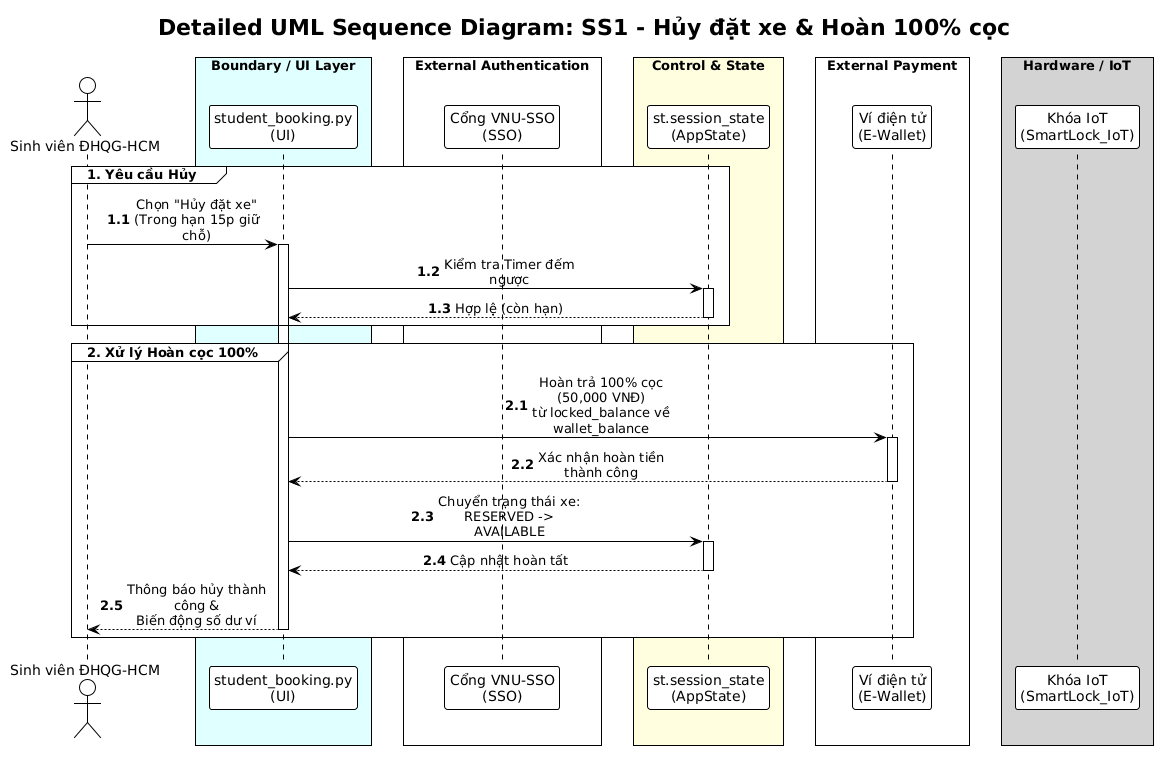
\includegraphics[width=0.88\textwidth,height=0.62\textheight,keepaspectratio]{Use-case detail-scenario/SS1/Sequence diagrams/UC_SS1_03_NguyenThanhDat_sequence.png}
    \caption{Sơ đồ Tuần tự Chi tiết -- UC\_SS1\_03 (Hủy đặt xe \& Hoàn cọc / Phạt No-show)}
    \label{fig:seq-ss1-03}
\end{figure}
\clearpage

% ------------------------------------------------------------
% 2.2 SS2 - Nguyễn Anh Tài
% ------------------------------------------------------------
\subsection{Phân hệ SS2: Đăng ký Sạc \& Đỗ xe cá nhân (Nguyễn Anh Tài)}

\subsubsection{UC\_SS2\_01: Đăng ký xe EV cá nhân}
\paragraph{Mô tả nghiệp vụ:} Sinh viên khai báo biển số xe, loại xe (VinFast, Dat Bike...), dung lượng pin và ảnh giấy đăng ký xe; hệ thống kiểm tra trùng lặp và lưu trữ hồ sơ phương tiện.
\begin{figure}[H]
    \centering
    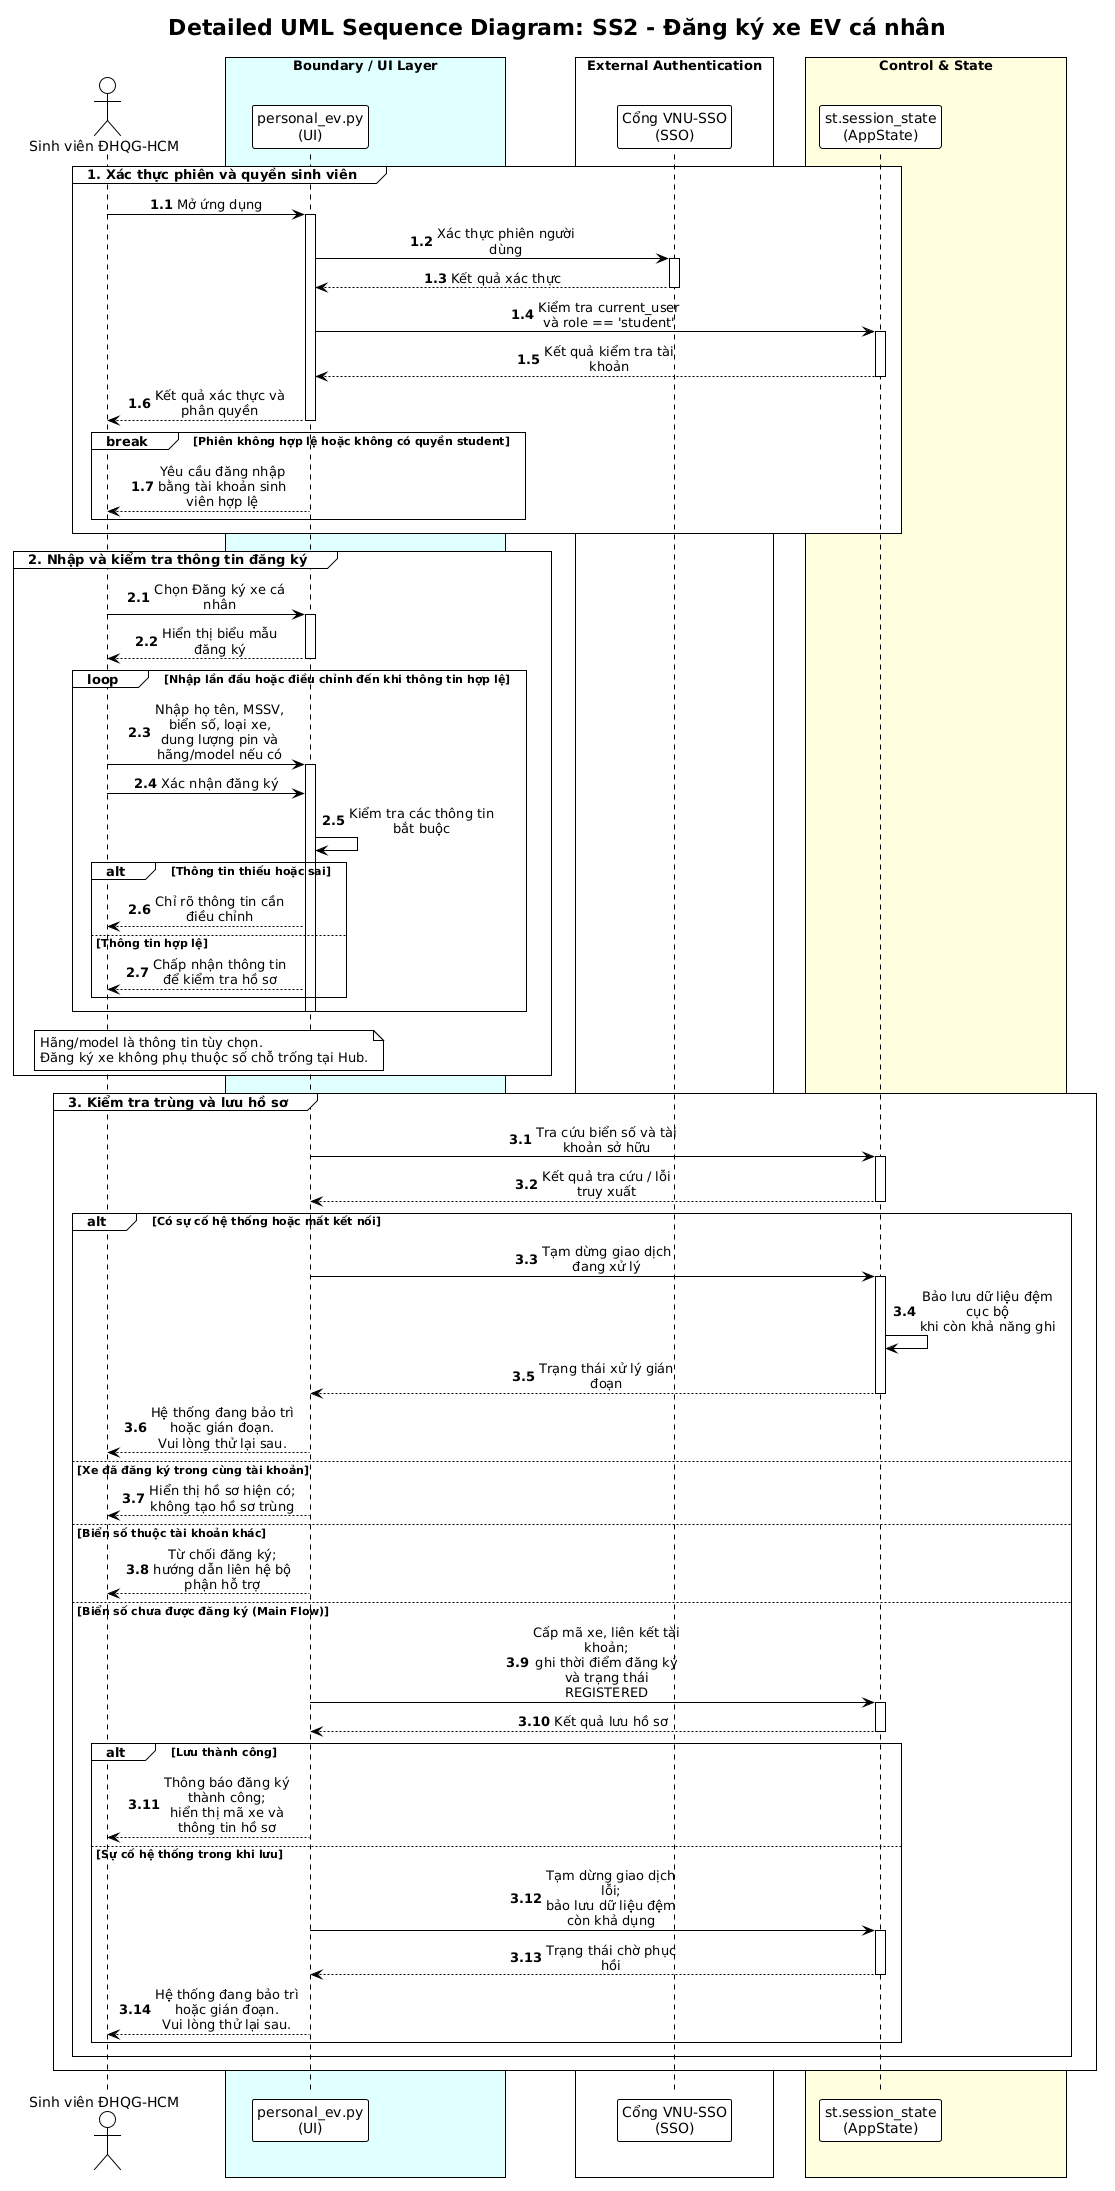
\includegraphics[width=0.88\textwidth,height=0.68\textheight,keepaspectratio]{Use-case detail-scenario/SS2/Sequence diagrams/UC_SS2_01_NguyenAnhTai_sequence.png}
    \caption{Sơ đồ Tuần tự Chi tiết -- UC\_SS2\_01 (Đăng ký xe EV cá nhân)}
    \label{fig:seq-ss2-01}
\end{figure}

\clearpage
\subsubsection{UC\_SS2\_02: Đặt chỗ đỗ và nhu cầu sạc xe EV cá nhân}
\paragraph{Mô tả nghiệp vụ:} Sinh viên chọn Hub đích, thời gian gửi xe và lựa chọn dịch vụ sạc có/không có sạc; hệ thống khóa giữ chỗ đỗ và ghi nhận nhu cầu sạc; việc cấp cổng thực hiện khi Check-in. Nhằm đảm bảo mọi nhãn thông điệp, điều kiện rẽ nhánh và ghi chú đều hiển thị rõ ràng, dễ đọc trên khổ trang in, sơ đồ được chia thành ba phần tiếp nối logic:
\begin{itemize}[nosep]
    \item \textbf{Phần 1 (Hình \ref{fig:seq-ss2-02-p1}):} Xác thực sinh viên qua SSO, lựa chọn xe cá nhân đã đăng ký, tra cứu khả dụng tại Hub và hiển thị dự toán biểu phí minh bạch.
    \item \textbf{Phần 2 (Hình \ref{fig:seq-ss2-02-p2}):} Khóa cọc 50.000 VNĐ, tạo đơn RESERVED và ghi nhận nhu cầu sạc; hạn Check-in tính từ giờ đến đã đặt.
    \item \textbf{Phần 3 (Hình \ref{fig:seq-ss2-02-p3}):} Các nhánh hủy đơn và hết hạn Check-in; giải phóng giữ chỗ và xử lý tiền cọc theo chính sách.
\end{itemize}

\begin{figure}[H]
    \centering
    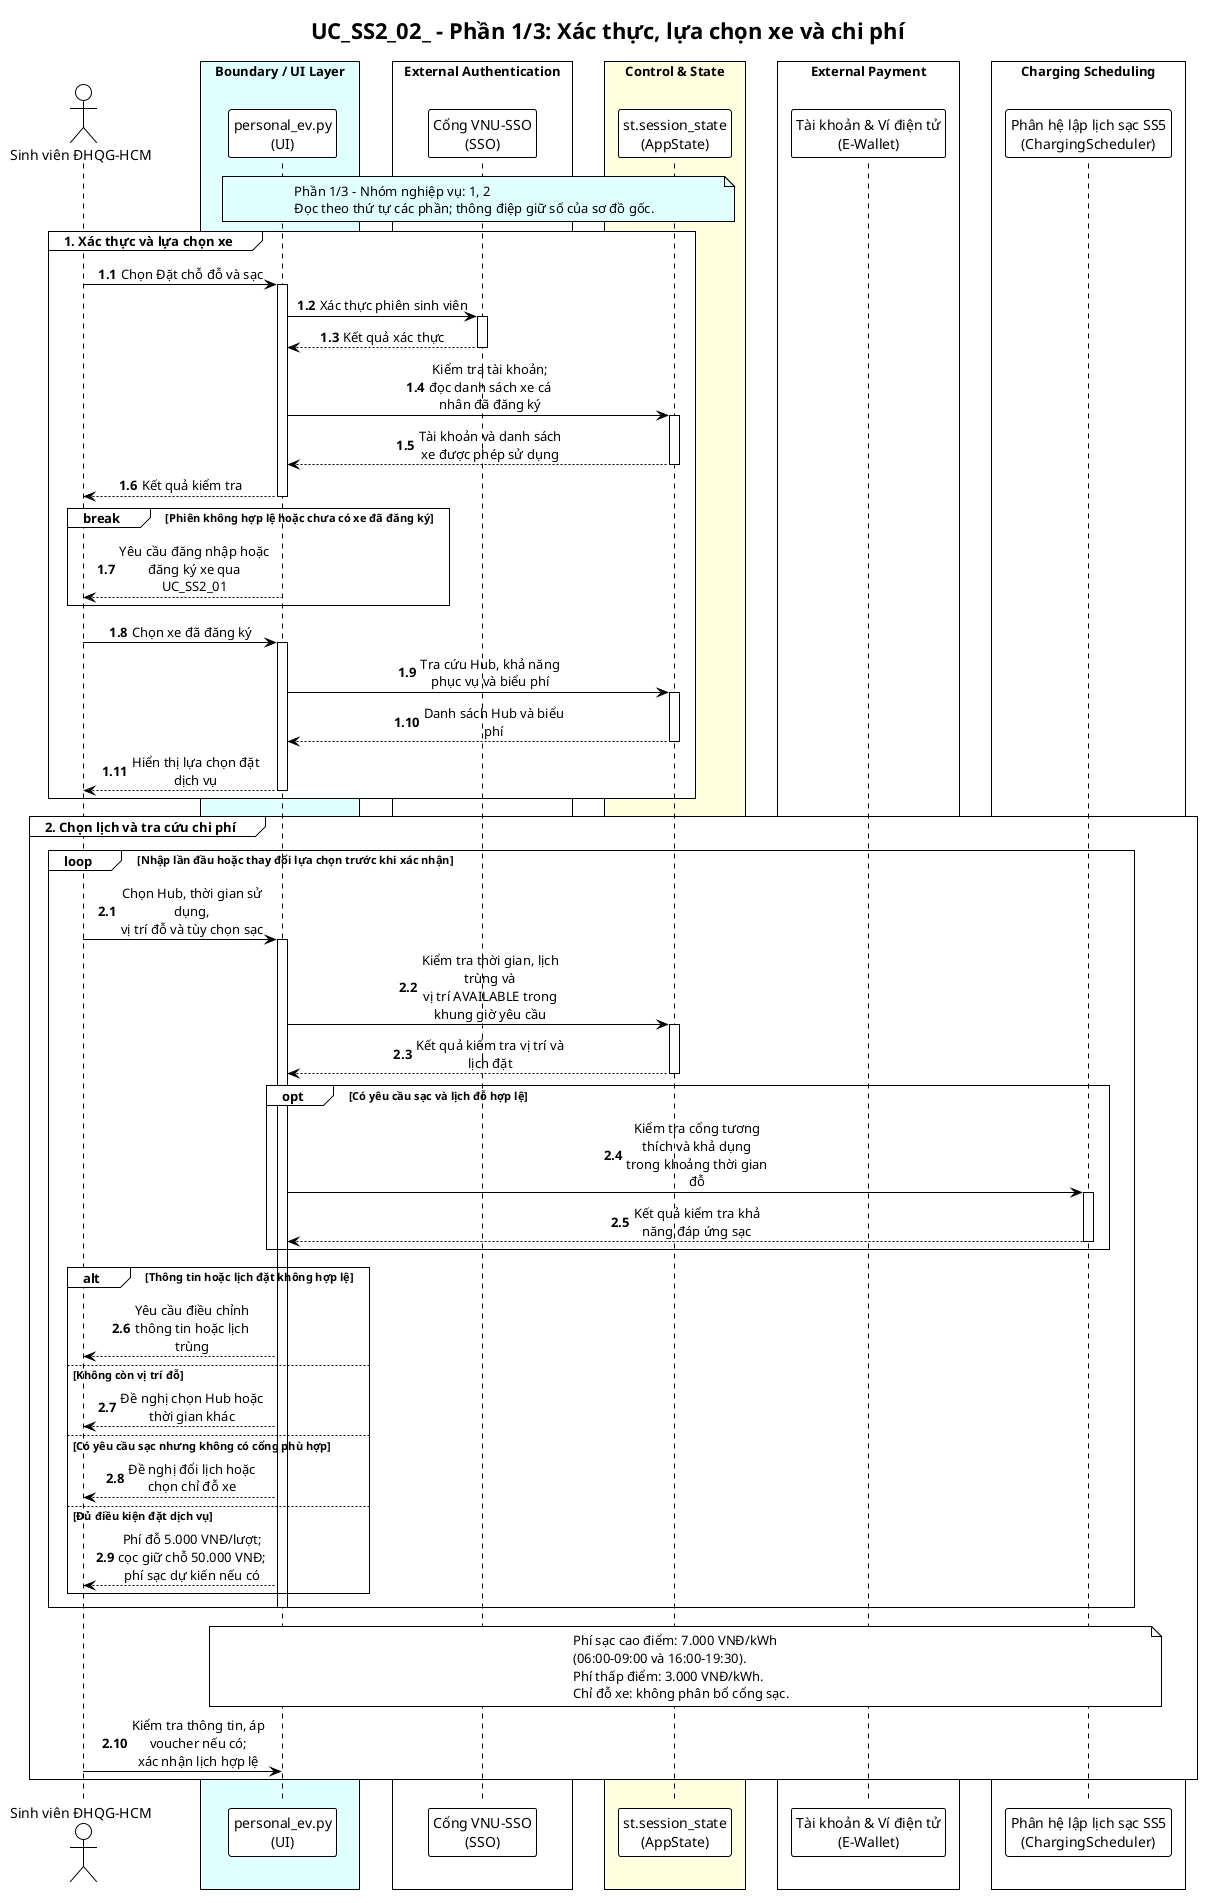
\includegraphics[width=0.88\textwidth,height=0.72\textheight,keepaspectratio]{Use-case detail-scenario/SS2/Sequence diagrams/UC_SS2_02_NguyenAnhTai_sequence_p1.png}
    \caption{Sơ đồ Tuần tự Chi tiết -- UC\_SS2\_02 (Phần 1: Xác thực, Lựa chọn xe \& Tra cứu chi phí)}
    \label{fig:seq-ss2-02-p1}
\end{figure}

\begin{figure}[H]
    \centering
    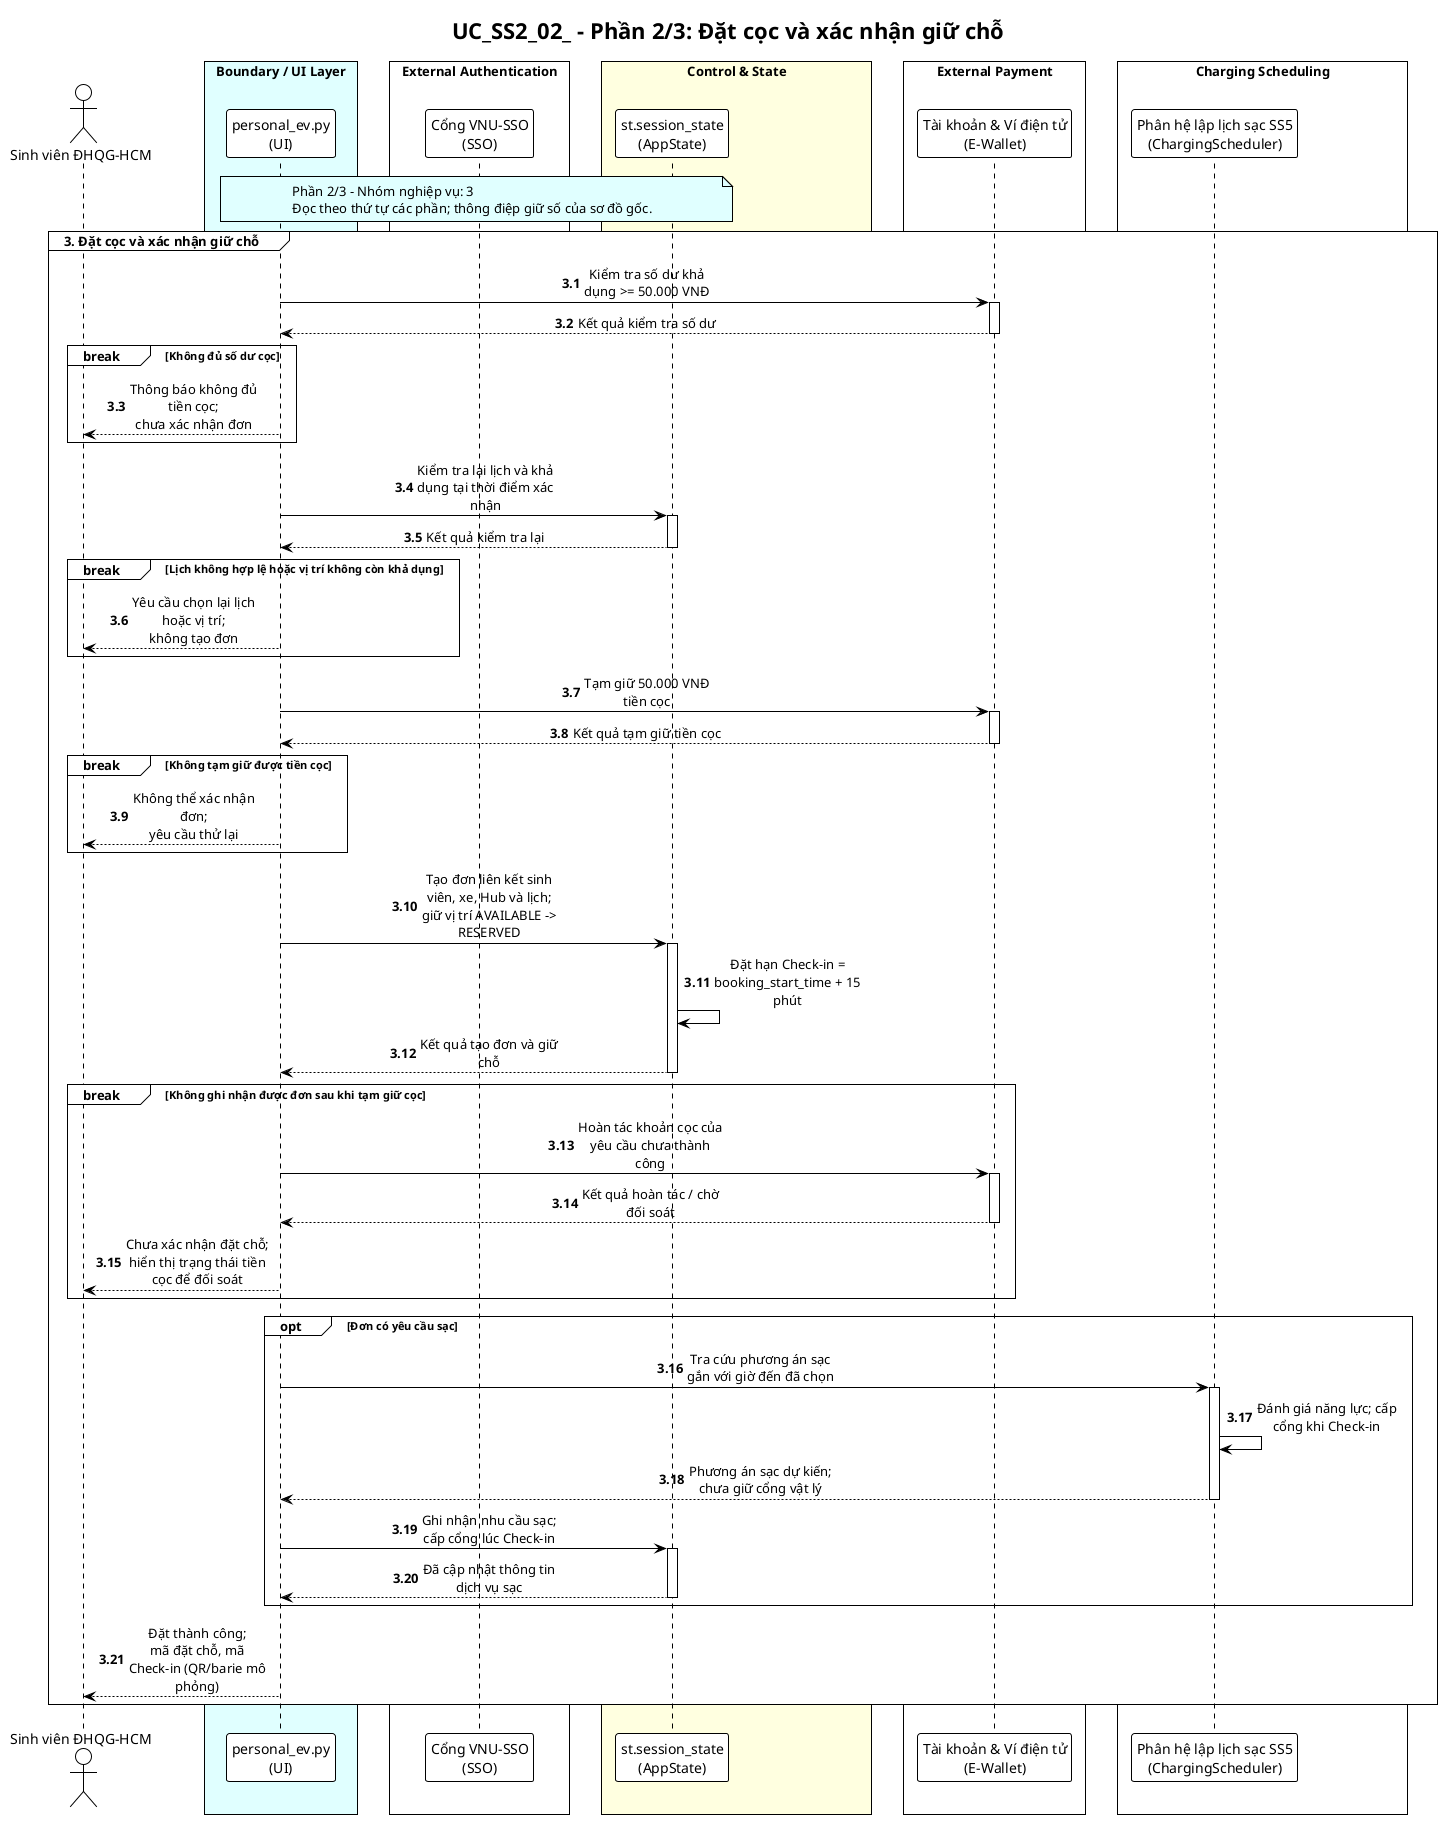
\includegraphics[width=0.88\textwidth,height=0.78\textheight,keepaspectratio]{Use-case detail-scenario/SS2/Sequence diagrams/UC_SS2_02_NguyenAnhTai_sequence_p2.png}
    \caption{Sơ đồ Tuần tự Chi tiết -- UC\_SS2\_02 (Phần 2: Đặt cọc \& Xác nhận giữ chỗ)}
    \label{fig:seq-ss2-02-p2}
\end{figure}

\begin{figure}[H]
    \centering
    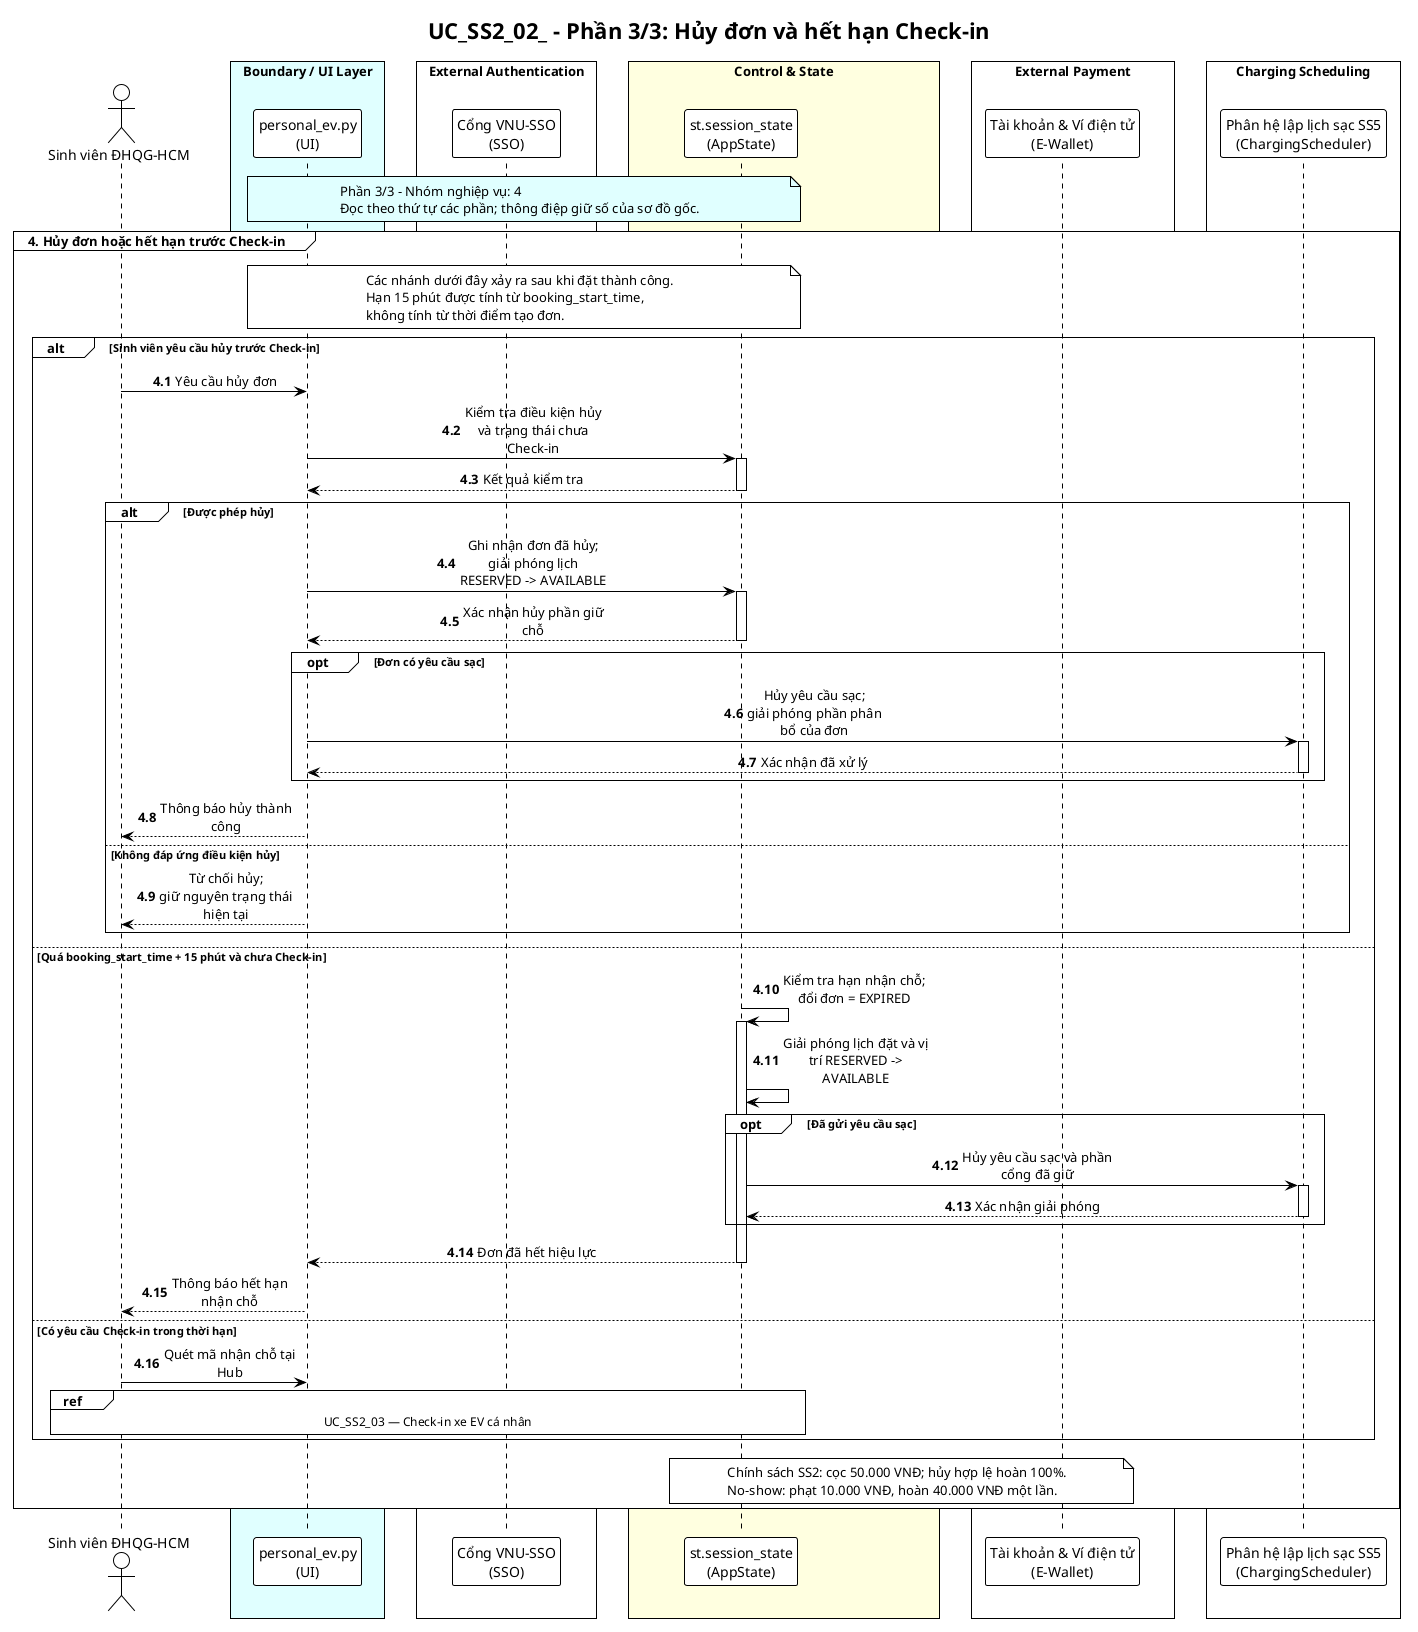
\includegraphics[width=0.92\textwidth,height=0.78\textheight,keepaspectratio]{Use-case detail-scenario/SS2/Sequence diagrams/UC_SS2_02_NguyenAnhTai_sequence_p3.png}
    \caption{Sơ đồ Tuần tự Chi tiết -- UC\_SS2\_02 (Phần 3: Hủy đơn \& Hết hạn Check-in)}
    \label{fig:seq-ss2-02-p3}
\end{figure}
\clearpage

\subsubsection{UC\_SS2\_03: Check-in xe EV cá nhân tại Hub}
\paragraph{Mô tả nghiệp vụ:} Hệ thống nhận diện biển số xe (hoặc mã QR/RFID) trùng khớp với phiên đặt trước, kích hoạt tín hiệu mở cổng tự động và chỉ dẫn sinh viên vào đúng vị trí slot đỗ/sạc.
\begin{figure}[H]
    \centering
    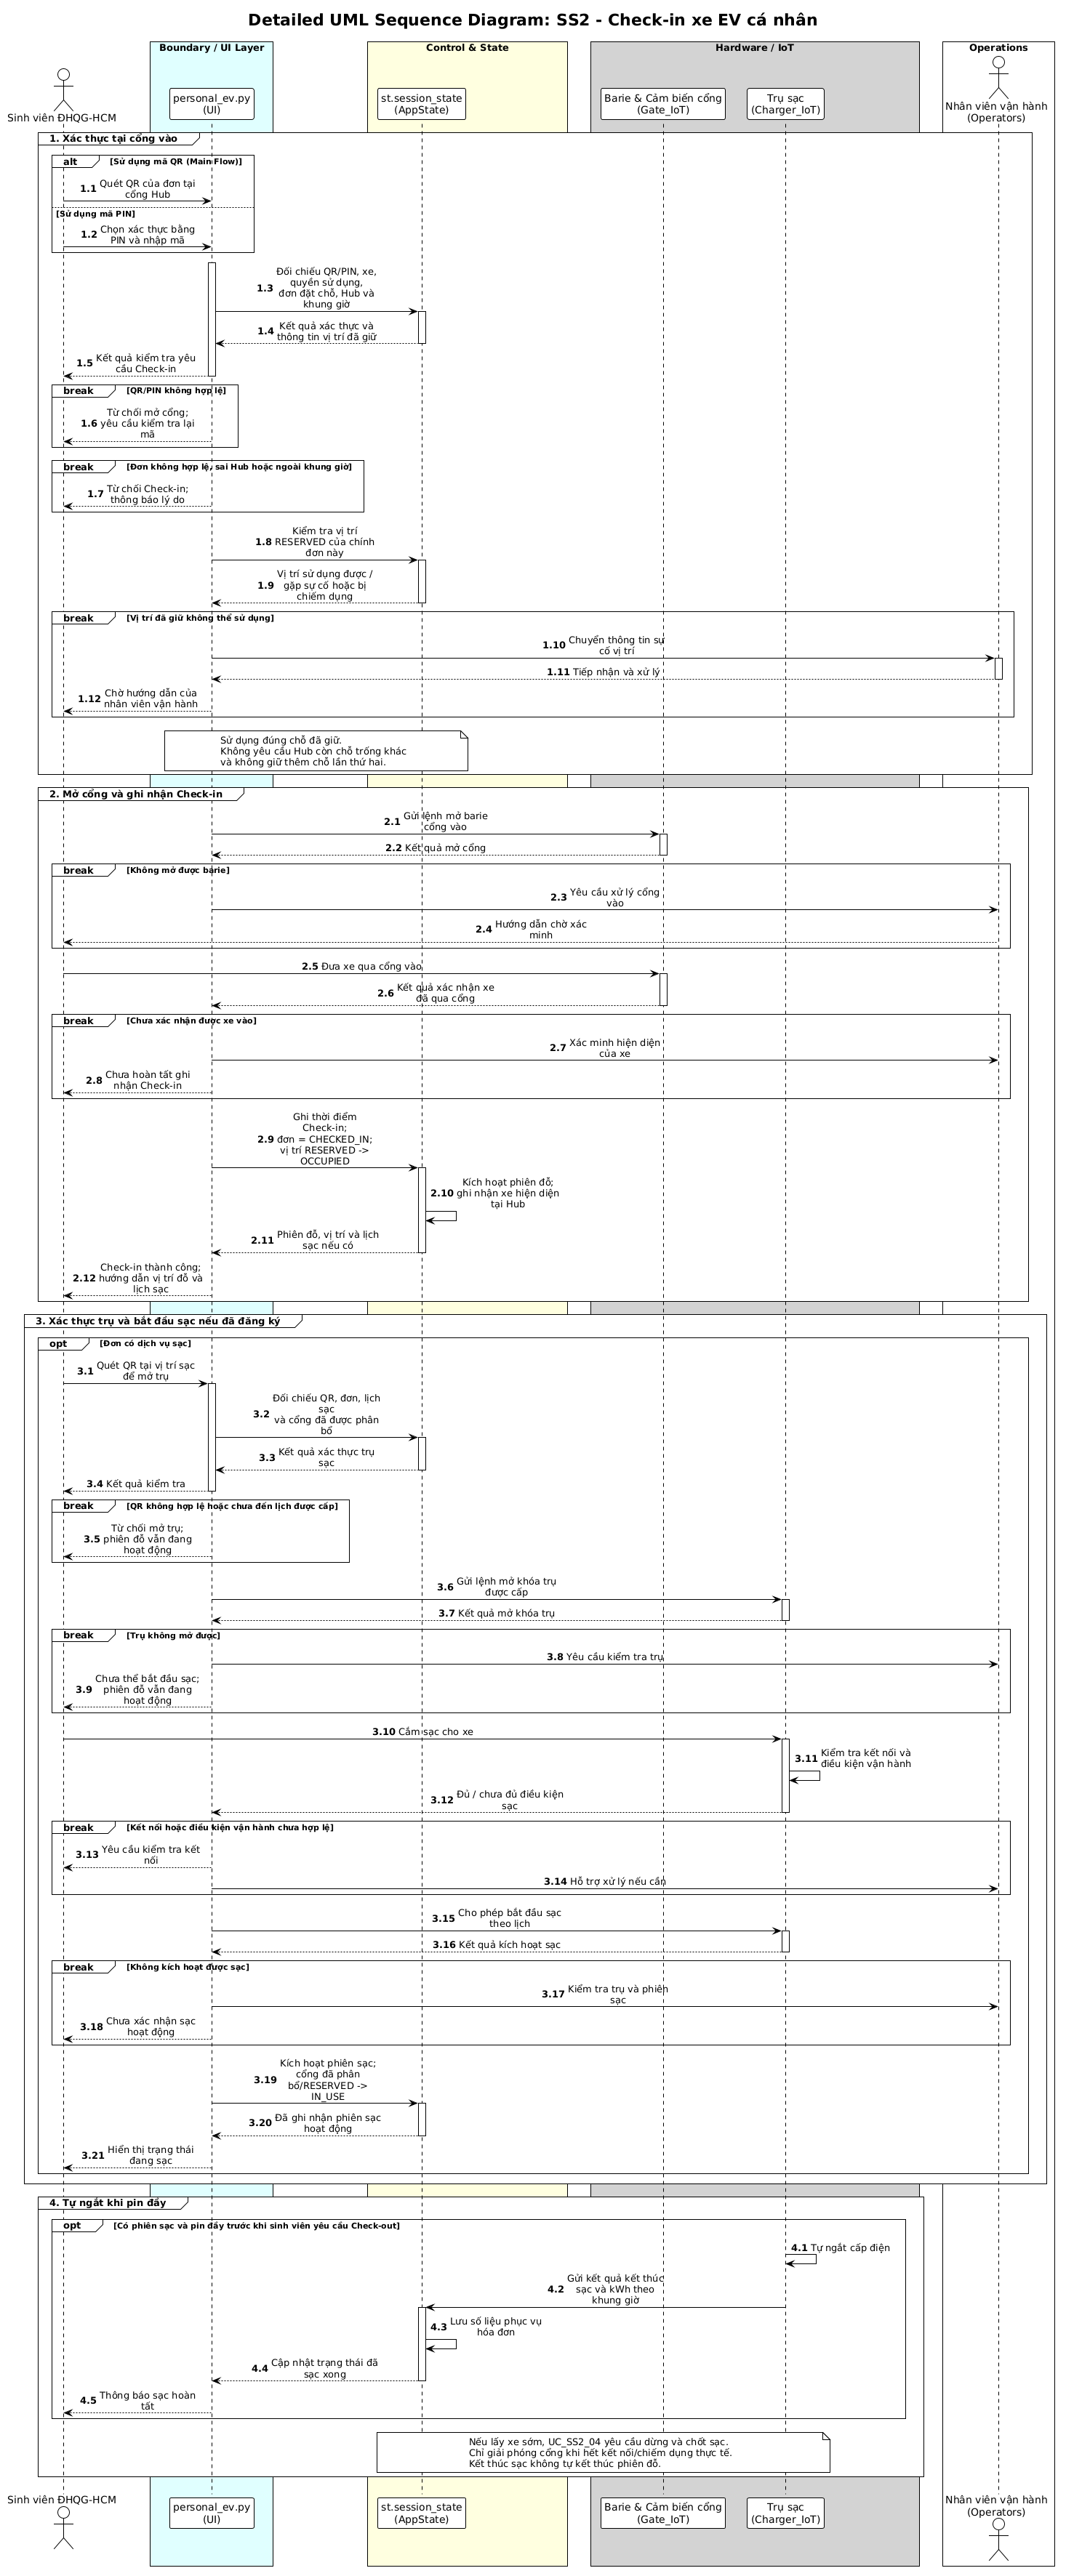
\includegraphics[width=0.88\textwidth,height=0.68\textheight,keepaspectratio]{Use-case detail-scenario/SS2/Sequence diagrams/UC_SS2_03_NguyenAnhTai_sequence.png}
    \caption{Sơ đồ Tuần tự Chi tiết -- UC\_SS2\_03 (Check-in xe EV cá nhân tại Hub)}
    \label{fig:seq-ss2-03}
\end{figure}

\clearpage
\subsubsection{UC\_SS2\_04: Check-out và thanh toán dịch vụ xe cá nhân}
\paragraph{Mô tả nghiệp vụ:} Khi sinh viên lấy xe ra, hệ thống tính toán tổng thời gian đỗ, điện năng tiêu thụ (kWh), tự động trừ ví điện tử và phát tín hiệu mở cổng bãi đỗ. Sơ đồ được trình bày qua ba phần tiếp nối:
\begin{itemize}[nosep]
    \item \textbf{Phần 1 (Hình \ref{fig:seq-ss2-04-p1}):} Xác thực phiên và lập hóa đơn tổng hợp phí đỗ, điện năng và quá giờ.
    \item \textbf{Phần 2 (Hình \ref{fig:seq-ss2-04-p2}):} Thanh toán qua ví mô phỏng, quyết toán cọc và xử lý các nhánh đối soát.
    \item \textbf{Phần 3 (Hình \ref{fig:seq-ss2-04-p3}):} Đối chiếu tại cổng ra, mở barie mô phỏng và giải phóng chỗ/cổng.
\end{itemize}

\begin{figure}[H]
    \centering
    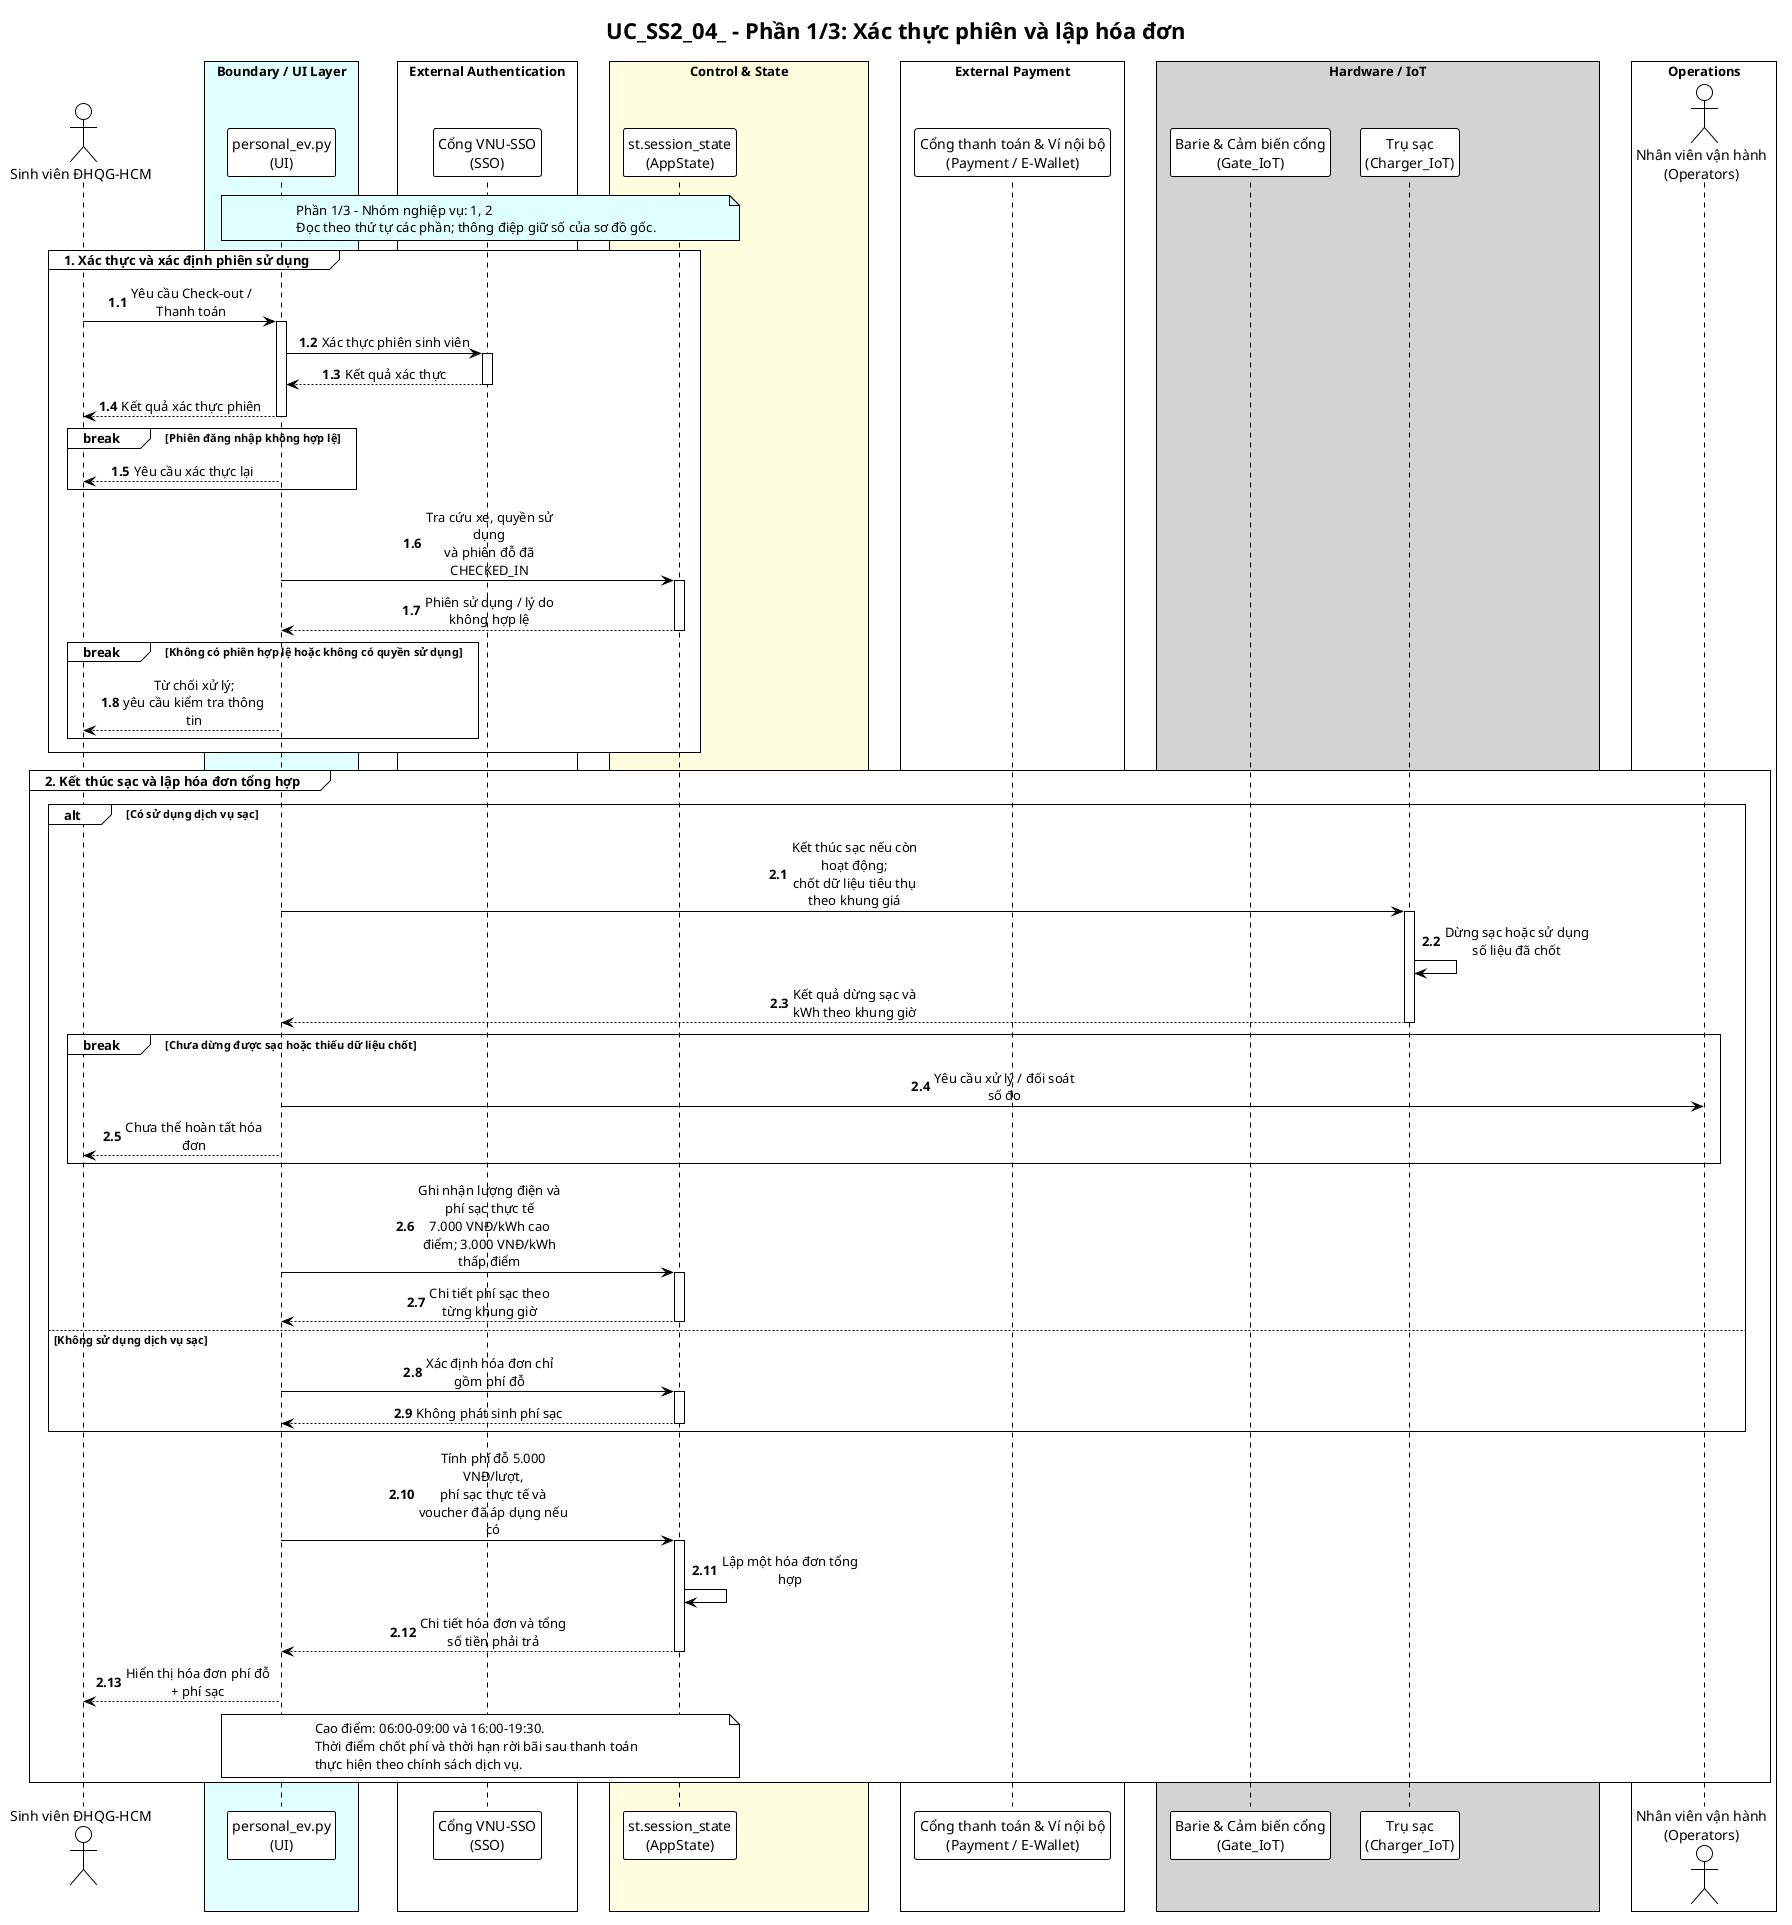
\includegraphics[width=0.88\textwidth,height=0.78\textheight,keepaspectratio]{Use-case detail-scenario/SS2/Sequence diagrams/UC_SS2_04_NguyenAnhTai_sequence_p1.png}
    \caption{Sơ đồ Tuần tự Chi tiết -- UC\_SS2\_04 (Phần 1: Xác thực phiên \& Lập hóa đơn)}
    \label{fig:seq-ss2-04-p1}
\end{figure}

\begin{figure}[H]
    \centering
    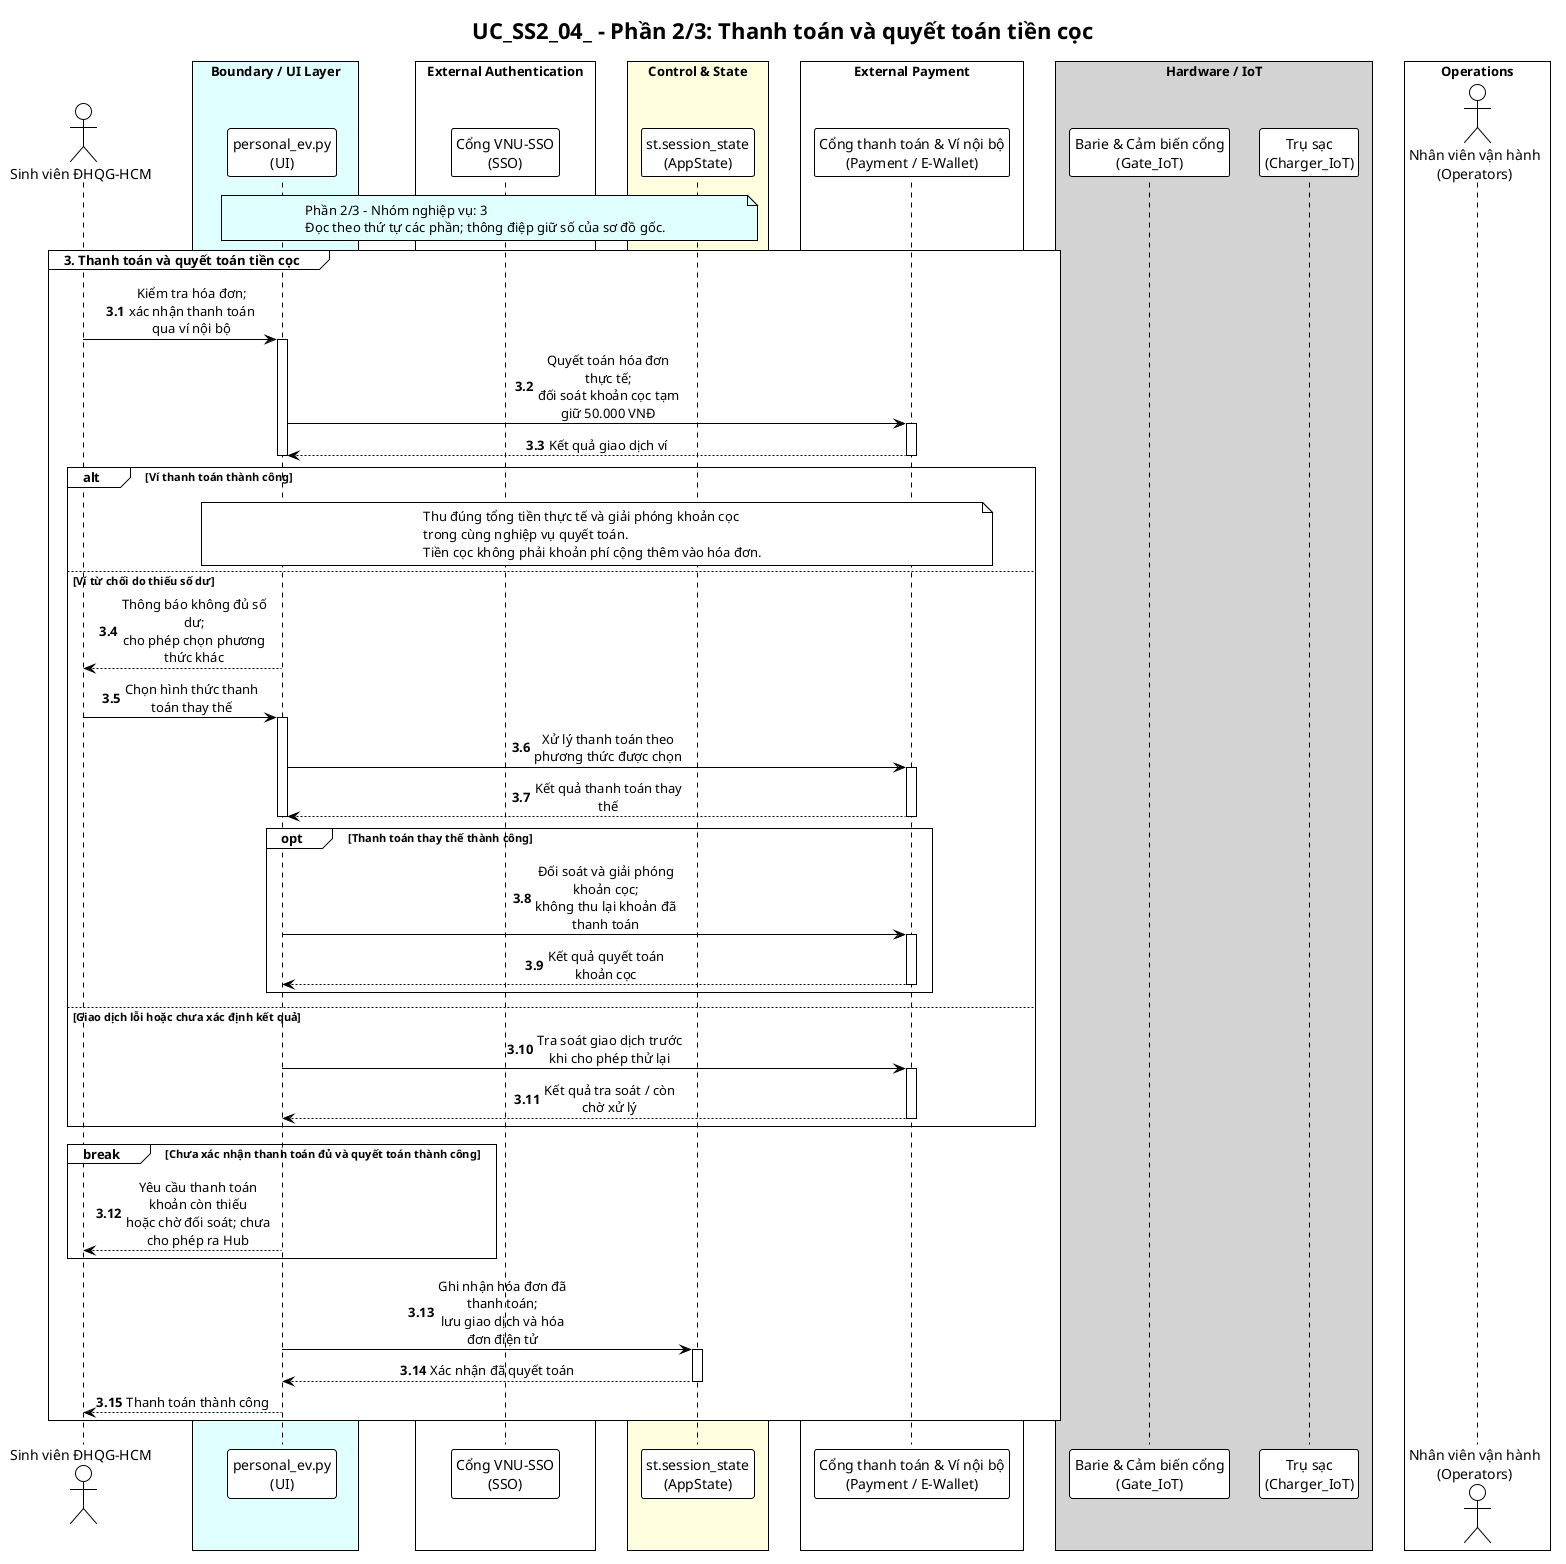
\includegraphics[width=0.88\textwidth,height=0.72\textheight,keepaspectratio]{Use-case detail-scenario/SS2/Sequence diagrams/UC_SS2_04_NguyenAnhTai_sequence_p2.png}
    \caption{Sơ đồ Tuần tự Chi tiết -- UC\_SS2\_04 (Phần 2: Thanh toán \& Quyết toán tiền cọc)}
    \label{fig:seq-ss2-04-p2}
\end{figure}

\begin{figure}[H]
    \centering
    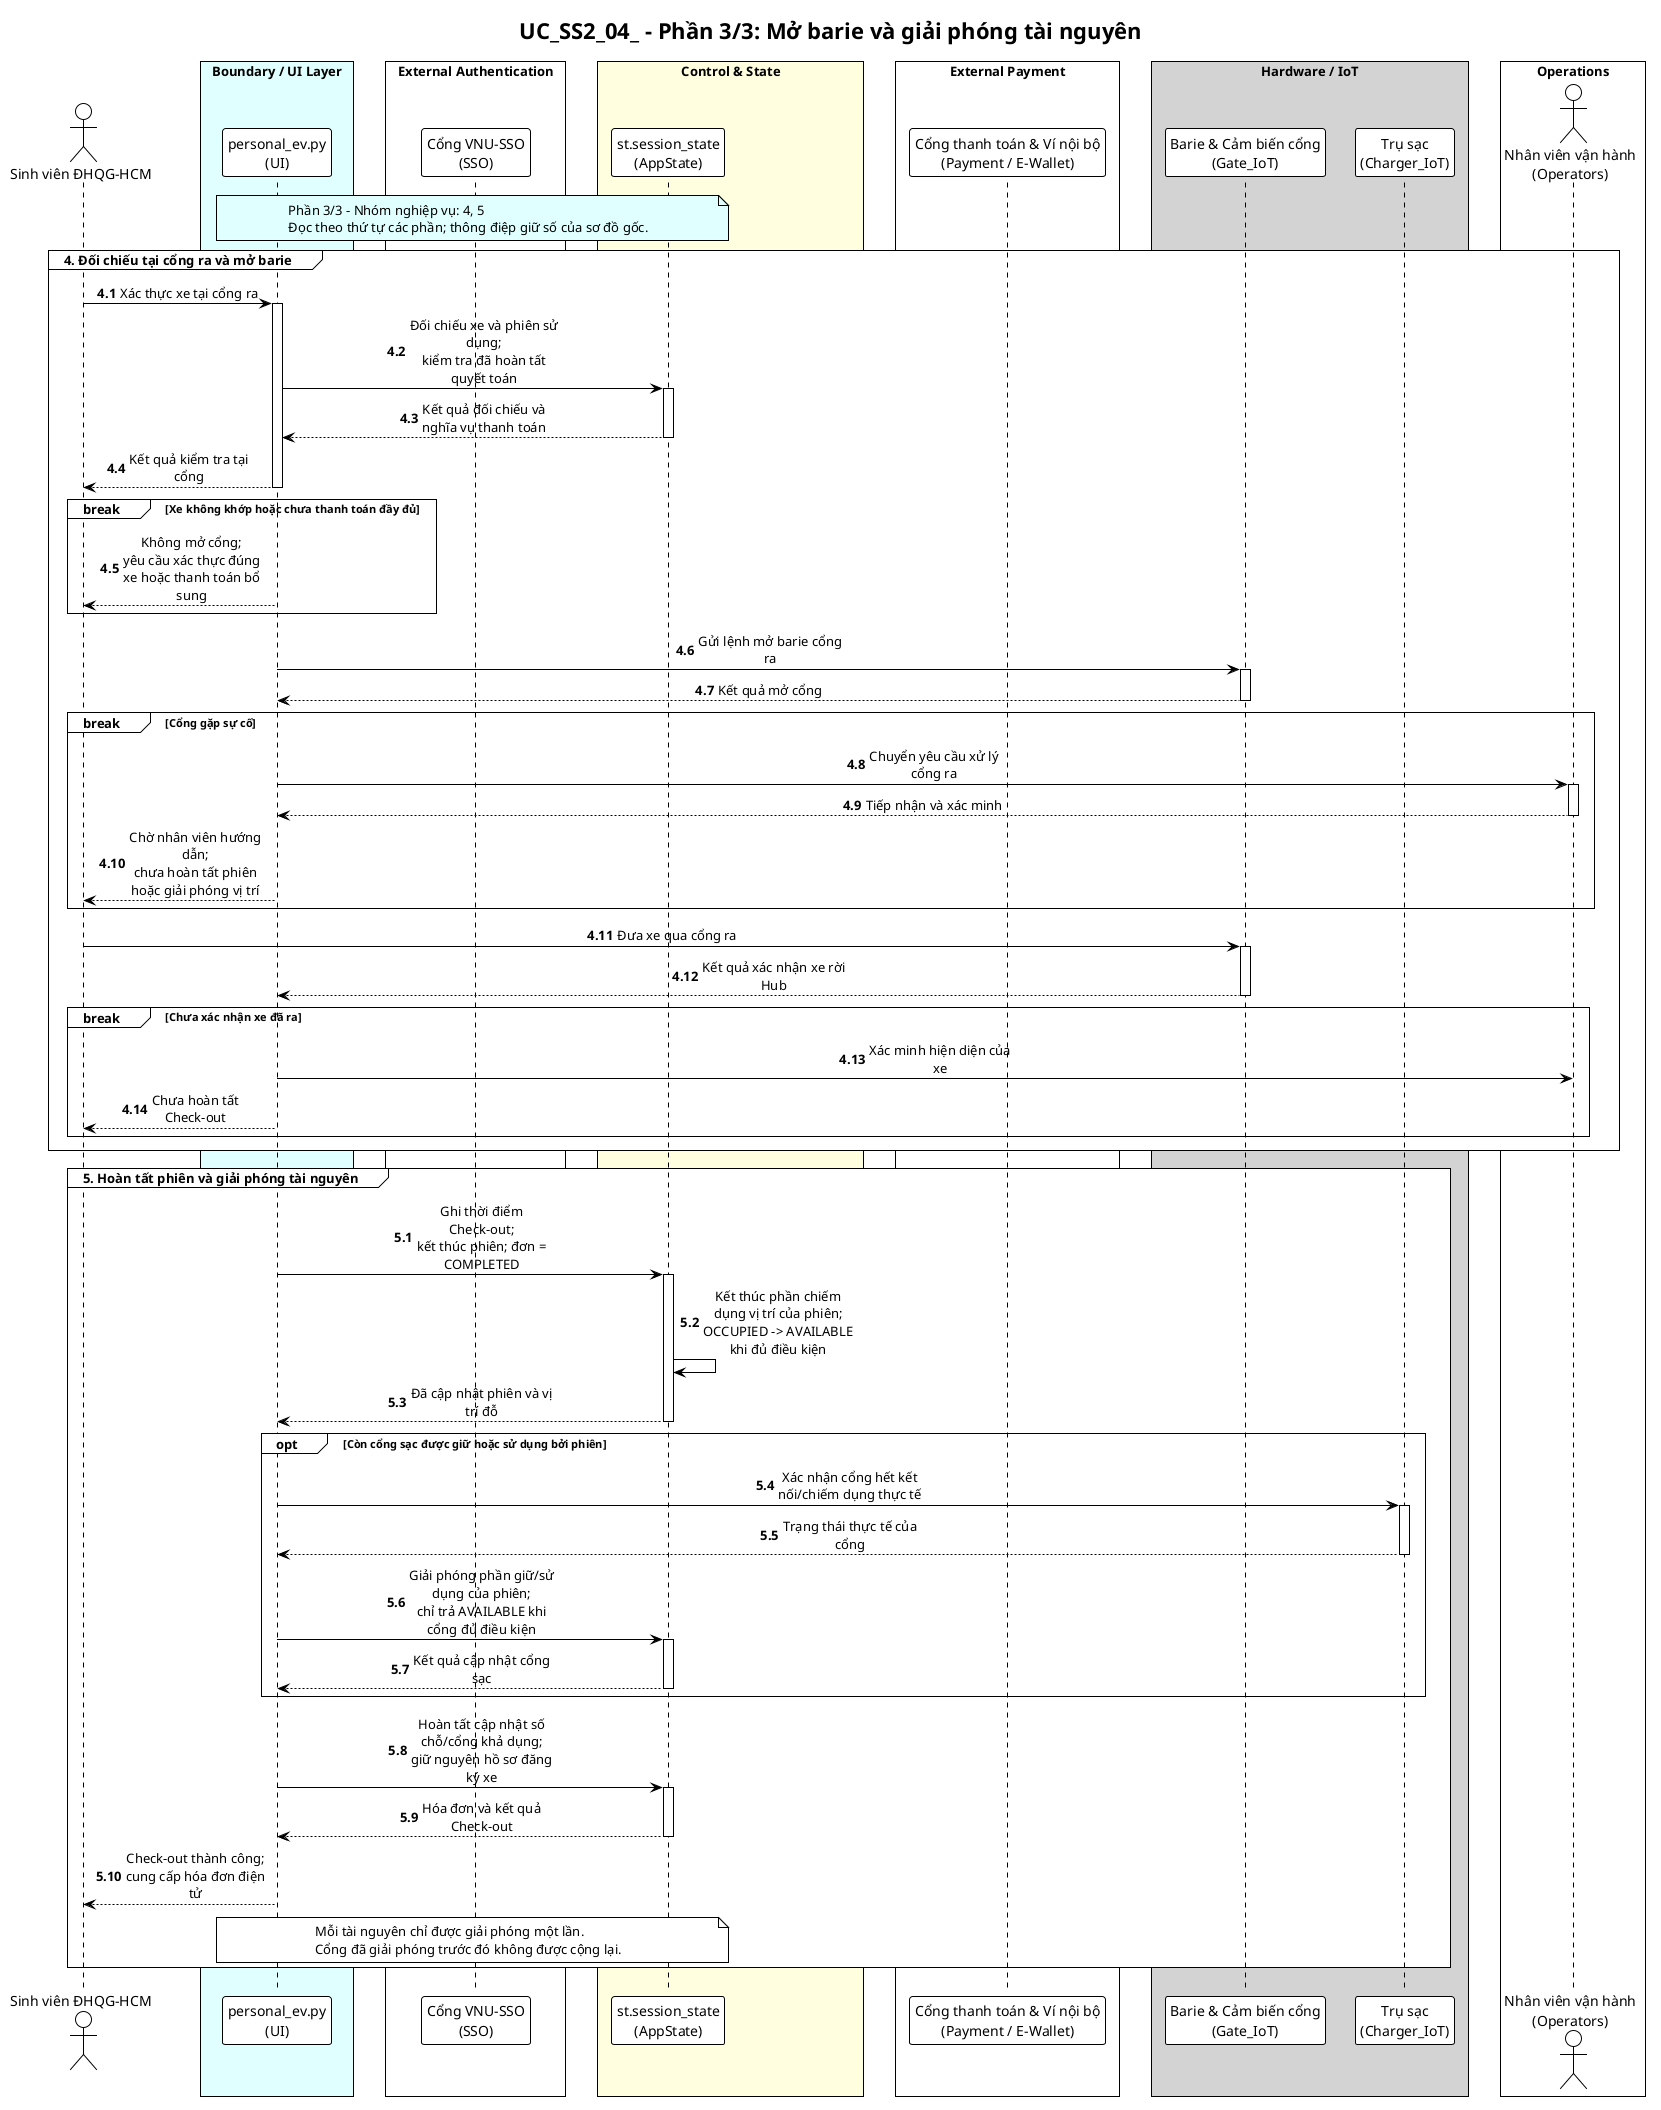
\includegraphics[width=0.92\textwidth,height=0.78\textheight,keepaspectratio]{Use-case detail-scenario/SS2/Sequence diagrams/UC_SS2_04_NguyenAnhTai_sequence_p3.png}
    \caption{Sơ đồ Tuần tự Chi tiết -- UC\_SS2\_04 (Phần 3: Mở barie \& Giải phóng tài nguyên)}
    \label{fig:seq-ss2-04-p3}
\end{figure}
\clearpage

% ------------------------------------------------------------
% 2.3 SS3 - Phạm Tiến Đạt
% ------------------------------------------------------------
\subsection{Phân hệ SS3: Giám sát Mạng lưới Hub (Phạm Tiến Đạt)}

\subsubsection{UC\_SS3\_01: Giám sát trạng thái Hub theo thời gian thực}
\paragraph{Mô tả nghiệp vụ:} Dashboard liên tục truy vấn dữ liệu từ cảm biến IoT (mô phỏng qua trạng thái xe) trong \texttt{st.session\_state["hubs"]}, tính toán tỷ lệ lấp đầy, số xe hoạt động và doanh thu tạm tính.
\begin{figure}[H]
    \centering
    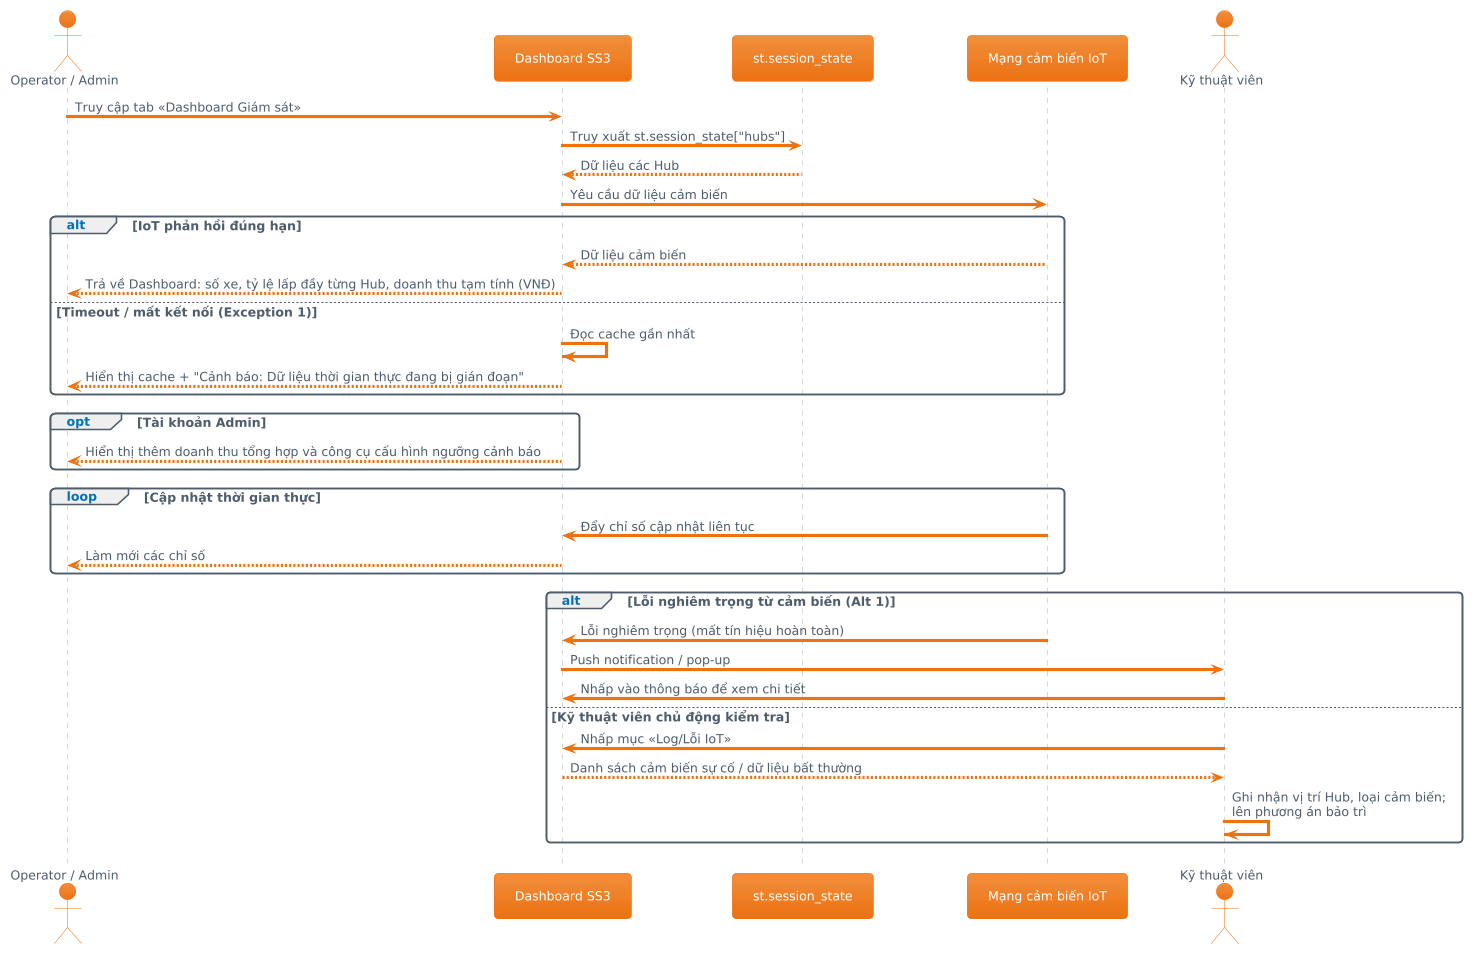
\includegraphics[width=0.88\textwidth,height=0.68\textheight,keepaspectratio]{Use-case detail-scenario/SS3/Sequence diagrams/UC_SS3_01_PhamTienDat_sequence.png}
    \caption{Sơ đồ Tuần tự Chi tiết -- UC\_SS3\_01 (Giám sát trạng thái Hub thời gian thực)}
    \label{fig:seq-ss3-01}
\end{figure}

\subsubsection{UC\_SS3\_02: Cảnh báo quá tải \& Đề xuất điều phối}
\paragraph{Mô tả nghiệp vụ:} Khi tỷ lệ lấp đầy tại một Hub vượt ngưỡng $\ge 85\%$, hệ thống tự động đẩy cảnh báo màu đỏ lên Dashboard và khởi tạo đề xuất lệnh điều xe sang phân hệ SS4.
\begin{figure}[H]
    \centering
    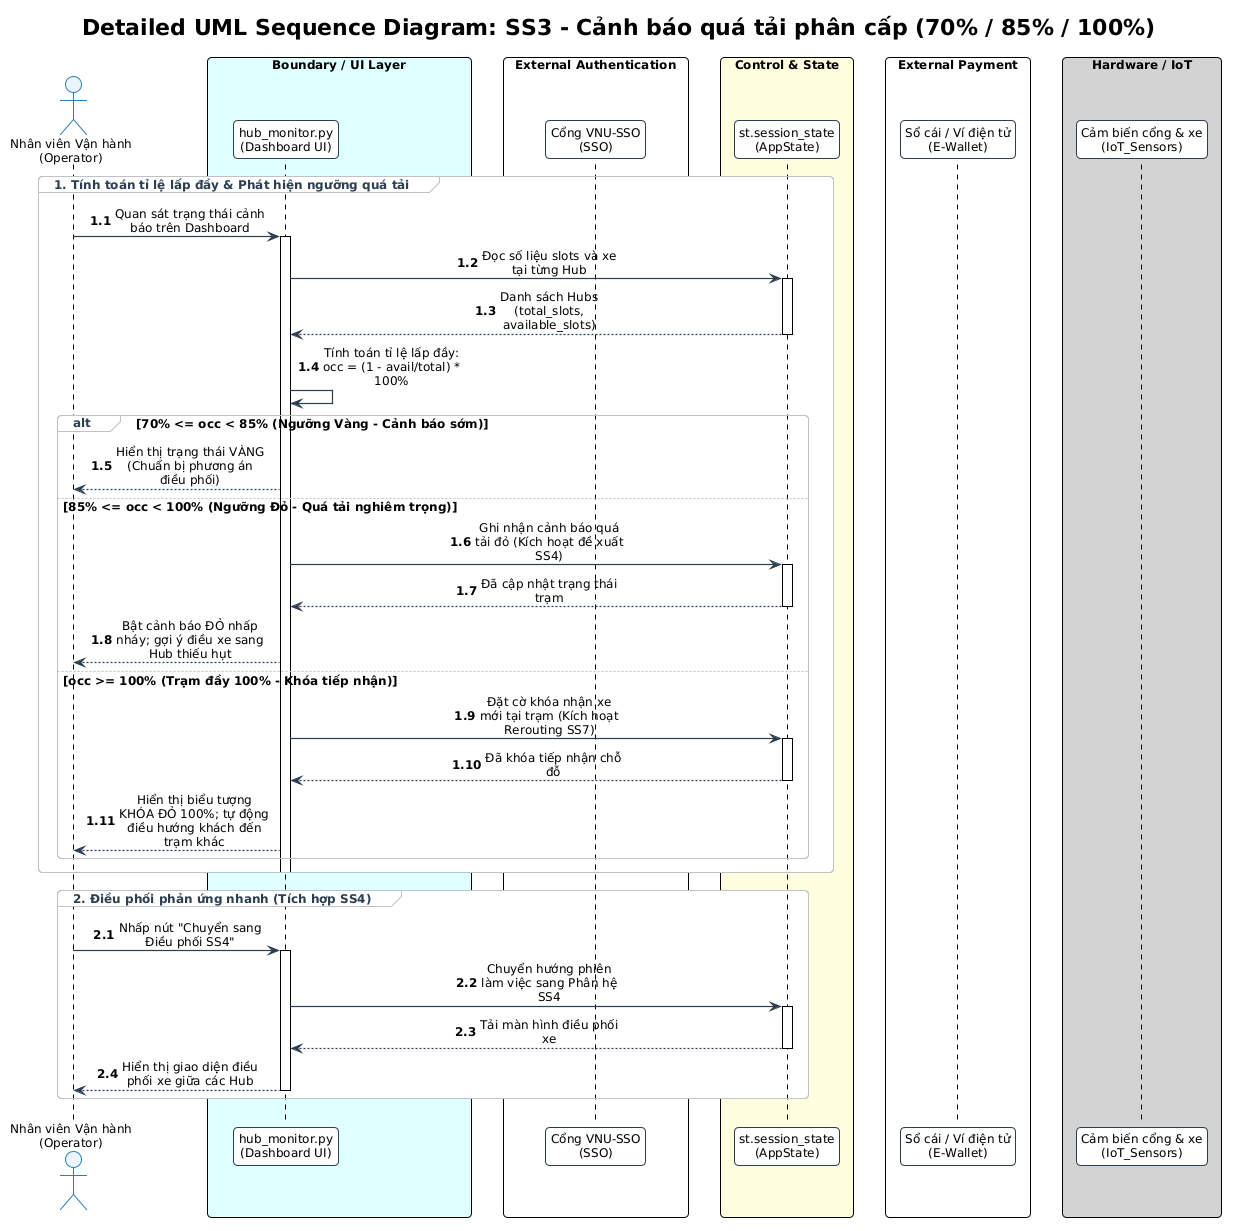
\includegraphics[width=0.88\textwidth,height=0.68\textheight,keepaspectratio]{Use-case detail-scenario/SS3/Sequence diagrams/UC_SS3_02_PhamTienDat_sequence.png}
    \caption{Sơ đồ Tuần tự Chi tiết -- UC\_SS3\_02 (Cảnh báo quá tải \& Đề xuất điều phối)}
    \label{fig:seq-ss3-02}
\end{figure}

% ------------------------------------------------------------
% 2.4 SS4 - Đặng Hoàng Quý Nhân
% ------------------------------------------------------------
\subsection{Phân hệ SS4: Điều phối \& Xử lý Sự cố (Đặng Hoàng Quý Nhân)}

\subsubsection{UC\_SS4\_01: Lập lệnh điều phối phương tiện giữa các Hub}
\paragraph{Mô tả nghiệp vụ:} Điều hành viên tiếp nhận cảnh báo quá tải, chọn Hub nguồn thừa xe và Hub đích thiếu xe, lập lệnh điều phối và phân bổ xe tải chuyên dụng thực hiện luân chuyển.
\begin{figure}[H]
    \centering
    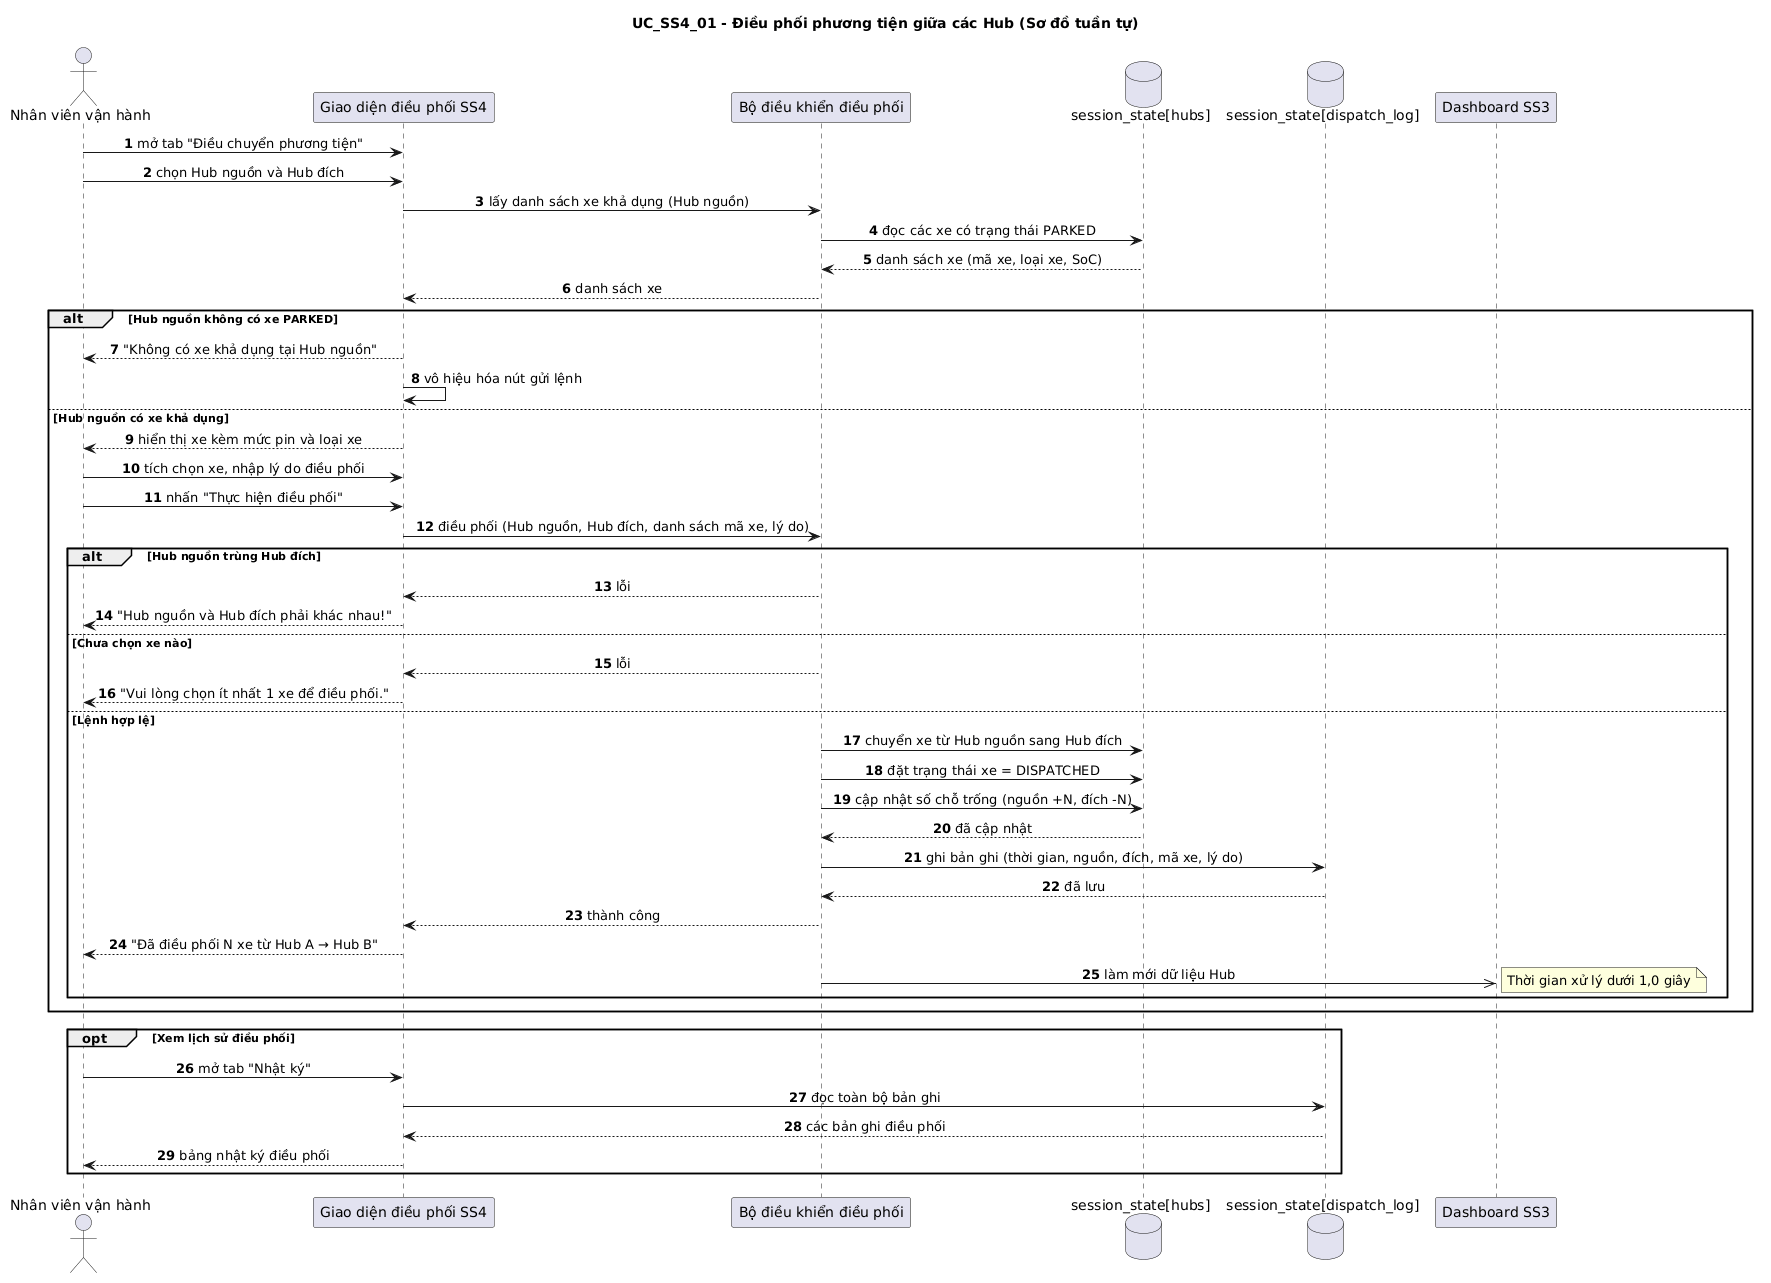
\includegraphics[width=0.88\textwidth,height=0.68\textheight,keepaspectratio]{Use-case detail-scenario/SS4/Sequence diagrams/UC_SS4_01_sequence.png}
    \caption{Sơ đồ Tuần tự Chi tiết -- UC\_SS4\_01 (Lập lệnh điều phối phương tiện)}
    \label{fig:seq-ss4-01}
\end{figure}

\subsubsection{UC\_SS4\_02: Báo cáo \& Xử lý sự cố kỹ thuật phương tiện}
\paragraph{Mô tả nghiệp vụ:} Khi có báo cáo hỏng xe từ sinh viên hoặc cảm biến pin quá nhiệt, hệ thống lập tức khóa xe khỏi danh sách cho thuê, phân công Kỹ thuật viên kiểm tra và sửa chữa.
\begin{figure}[H]
    \centering
    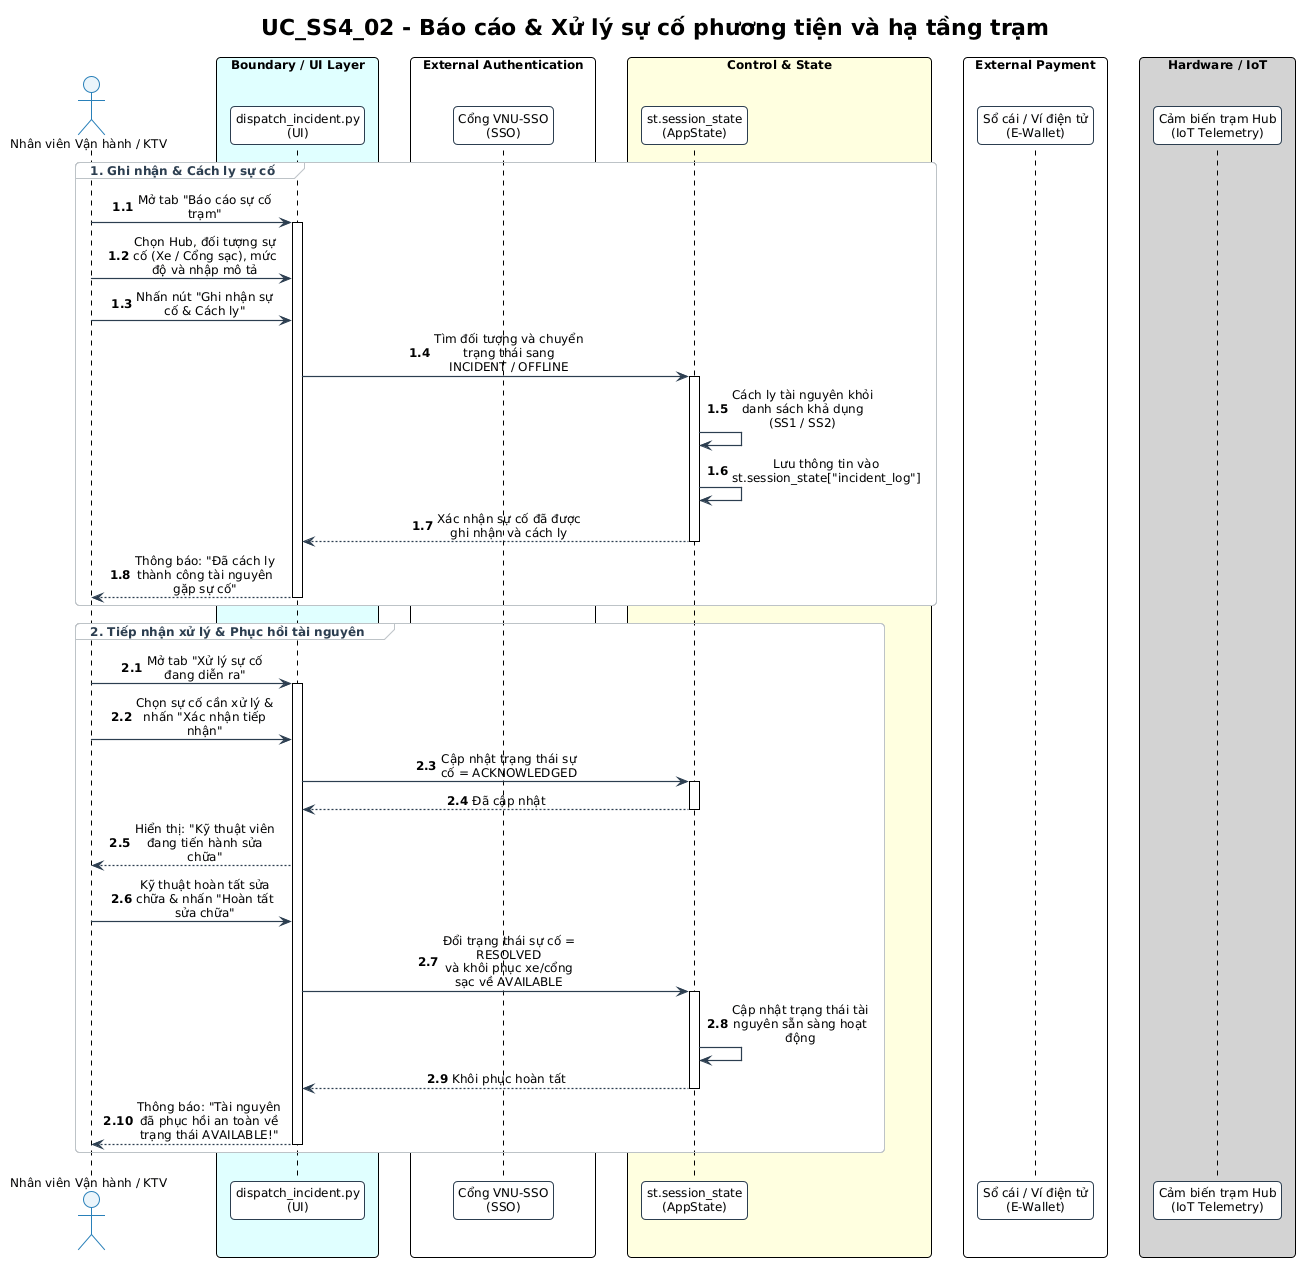
\includegraphics[width=0.88\textwidth,height=0.68\textheight,keepaspectratio]{Use-case detail-scenario/SS4/Sequence diagrams/UC_SS4_02_sequence.png}
    \caption{Sơ đồ Tuần tự Chi tiết -- UC\_SS4\_02 (Báo cáo \& Xử lý sự cố kỹ thuật xe)}
    \label{fig:seq-ss4-02}
\end{figure}

% ------------------------------------------------------------
% 2.5 SS5 - Dương Đăng Khoa
% ------------------------------------------------------------
\subsection{Phân hệ SS5: Lập lịch Sạc Thông minh (Dương Đăng Khoa)}

\subsubsection{UC\_SS5\_01: Lập lịch ưu tiên sạc tự động}
\paragraph{Mô tả nghiệp vụ:} Thuật toán tối ưu hóa lịch sạc (\texttt{SmartChargingScheduler}) tính toán điểm ưu tiên đa mục tiêu cho từng phương tiện trong hàng đợi dựa trên: mức pin khẩn cấp ($\text{SoC} < 20\%$), có lịch đặt xe của sinh viên ($\text{Booking}$), pin dưới trung bình ($\text{SoC} < 50\%$) và độ suy giảm pin tuyến tính. Hệ thống tự động phân bổ nguồn sạc trước cho các phương tiện có điểm ưu tiên cao nhất.
\begin{figure}[H]
    \centering
    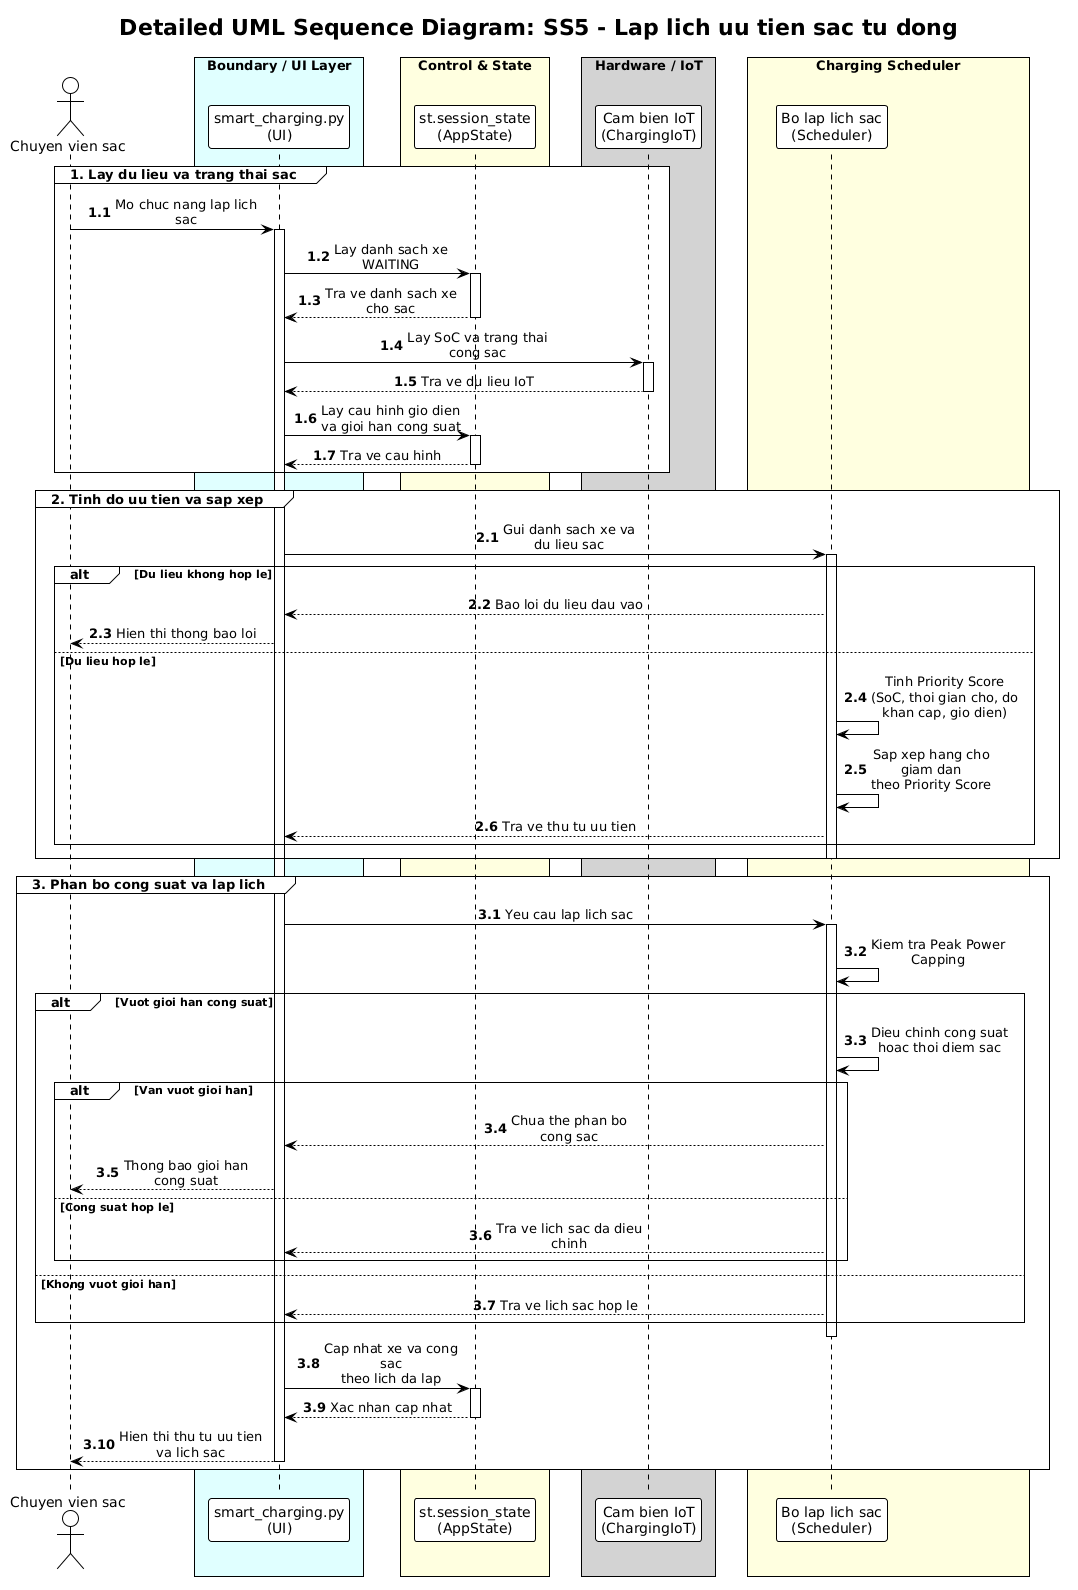
\includegraphics[width=0.88\textwidth,height=0.68\textheight,keepaspectratio]{Use-case detail-scenario/SS5/Sequence diagrams/UC_SS5_01_DuongDangKhoa_sequence.png}
    \caption{Sơ đồ Tuần tự Chi tiết -- UC\_SS5\_01 (Lập lịch ưu tiên sạc tự động)}
    \label{fig:seq-ss5-01}
\end{figure}

\subsubsection{UC\_SS5\_02: Giám sát hàng đợi sạc \& Phí chiếm dụng}
\paragraph{Mô tả nghiệp vụ:} Khi xe sạc đầy 100\%, hệ thống ngắt sạc và gửi thông báo cho sinh viên kèm thời gian ân hạn 15 phút. Nếu quá 15 phút xe chưa được rút, hệ thống bắt đầu tính phí phạt chiếm dụng trụ sạc 10.000đ/15 phút.
\begin{figure}[H]
    \centering
    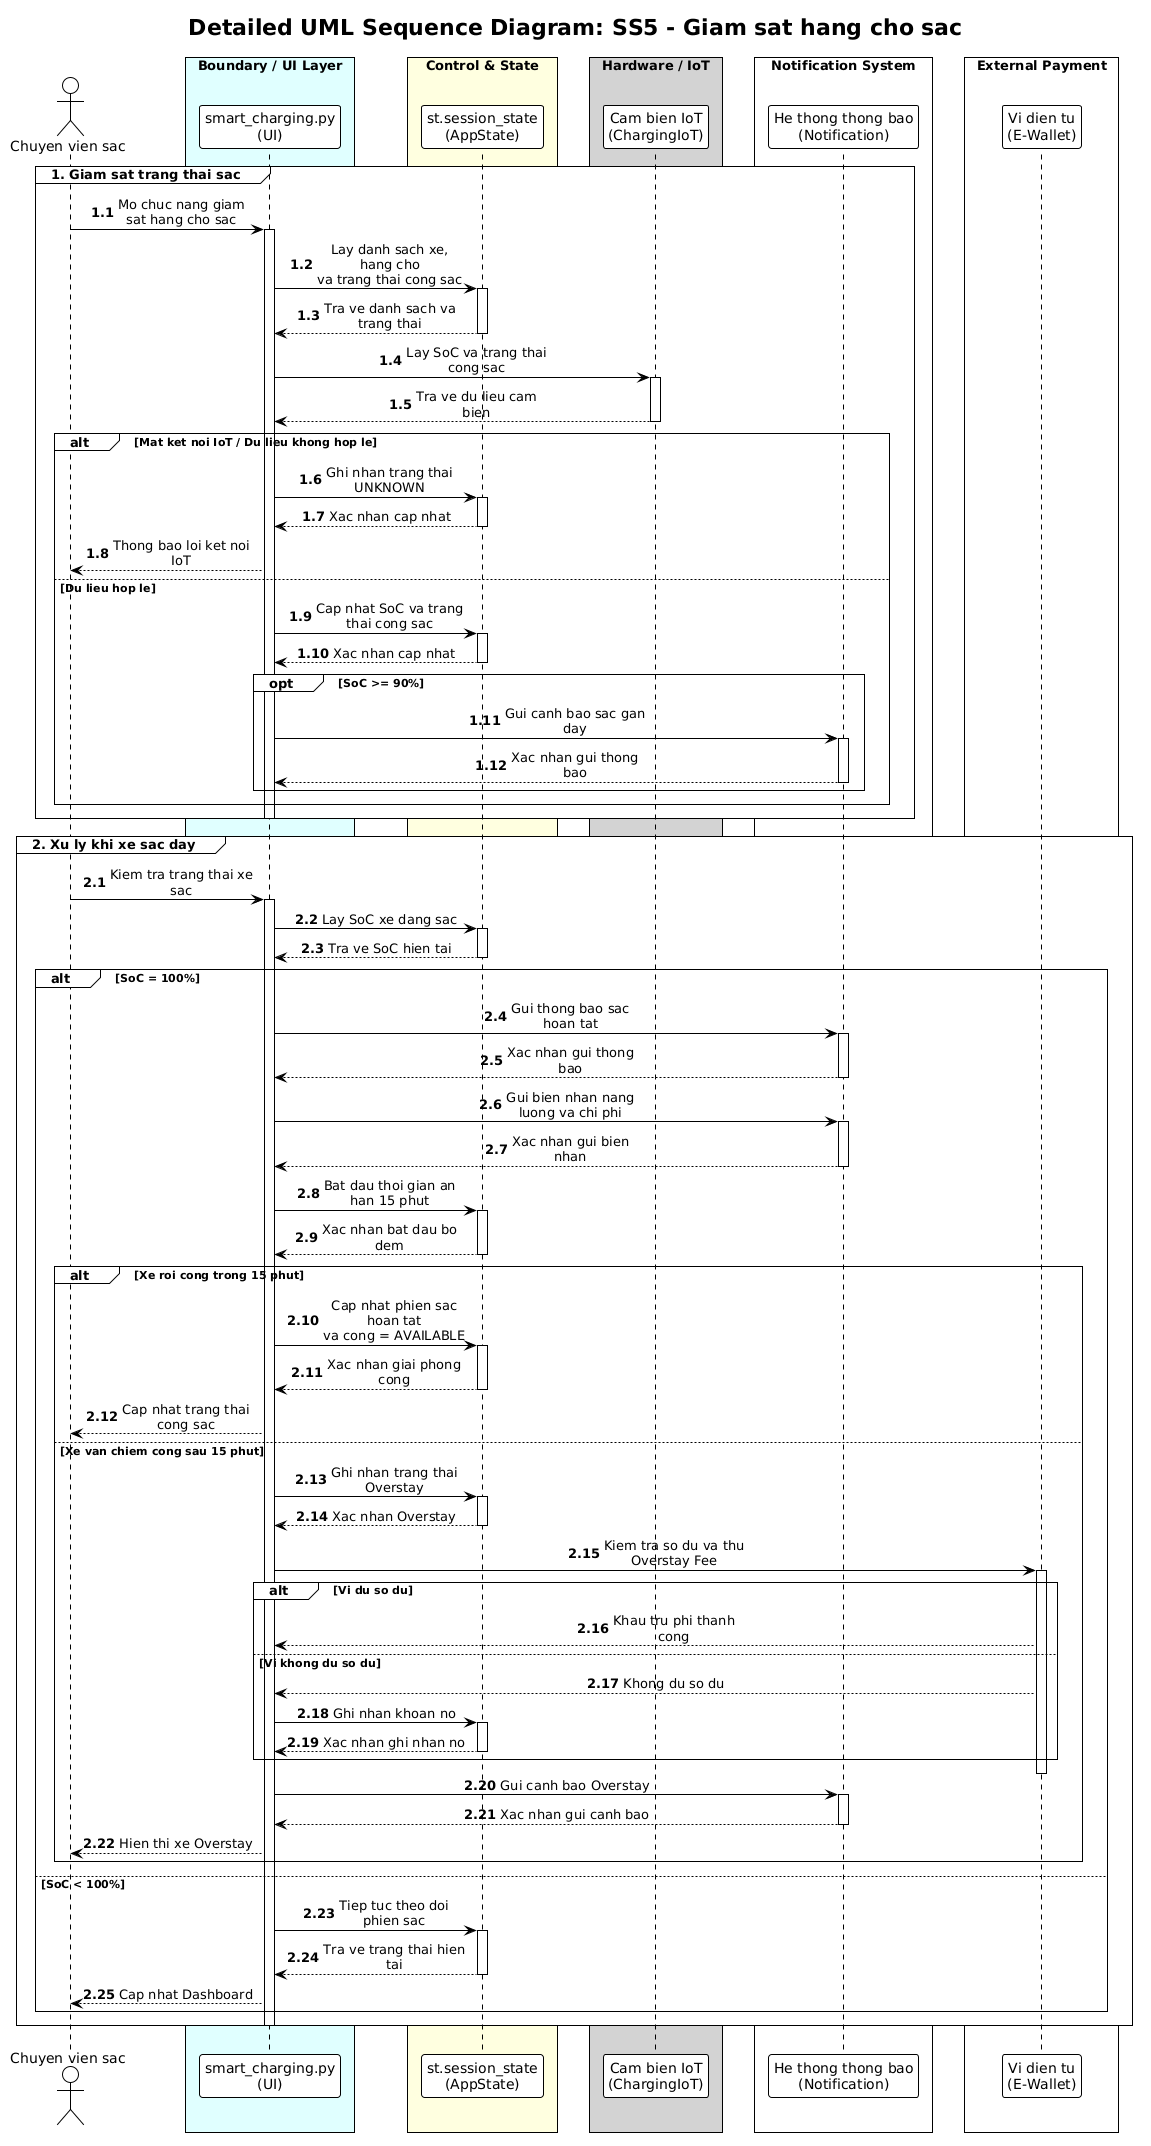
\includegraphics[width=0.88\textwidth,height=0.68\textheight,keepaspectratio]{Use-case detail-scenario/SS5/Sequence diagrams/UC_SS5_02_DuongDangKhoa_sequence.png}
    \caption{Sơ đồ Tuần tự Chi tiết -- UC\_SS5\_02 (Giám sát hàng đợi sạc \& Phí chiếm dụng)}
    \label{fig:seq-ss5-02}
\end{figure}

% ------------------------------------------------------------
% 2.6 SS6 - Hoàng Văn Tấn
% ------------------------------------------------------------
\subsection{Phân hệ SS6: Mô phỏng What-if Nhu cầu (Hoàng Văn Tấn)}

\subsubsection{UC\_SS6\_01: Mô phỏng đợt tăng đột biến hành khách Metro (Metro Surge)}
\paragraph{Mô tả nghiệp vụ:} Nhà phân tích / Người vận hành Hub thiết lập tham số đợt xả khách tại ga Metro ĐHQG-HCM (Hub KTX Khu B), động cơ mô phỏng \texttt{HubEventSimulator} thực hiện biến đổi trên bản sao sâu (\texttt{deepcopy}) dữ liệu trạm, tính toán áp lực thiếu xe và đề xuất lượng xe cần điều phối bù sang SS4.
\begin{figure}[H]
    \centering
    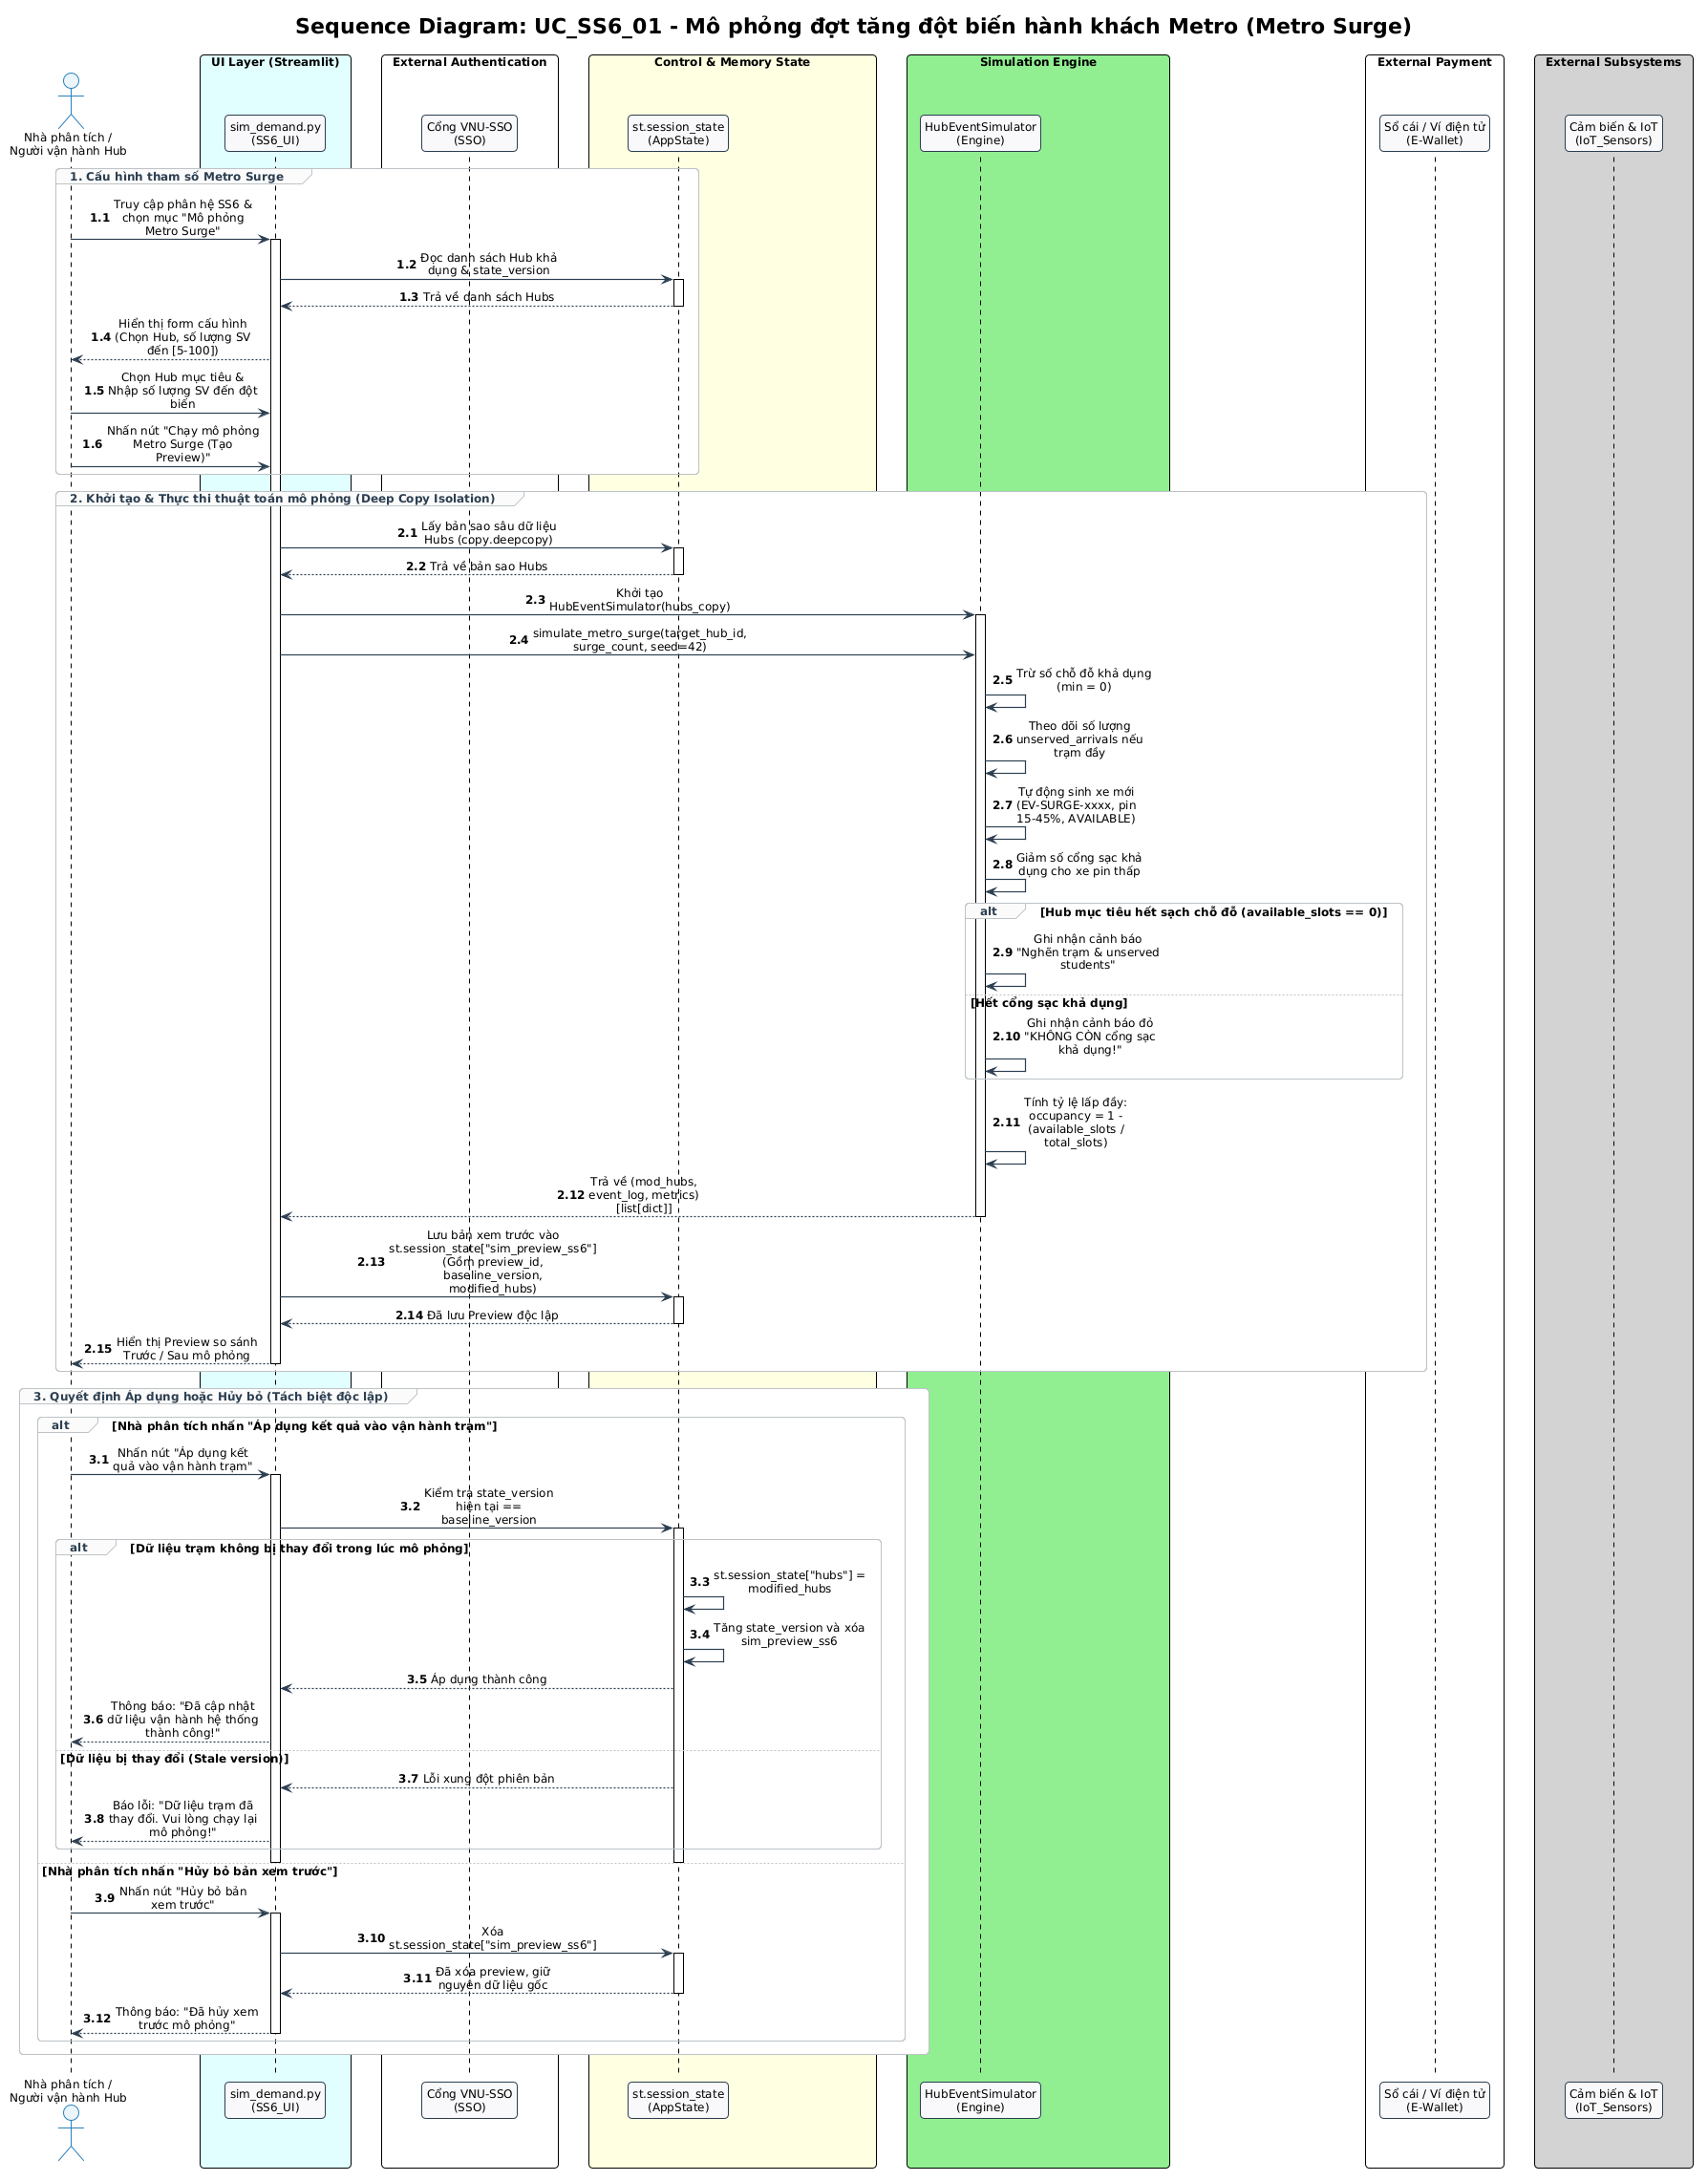
\includegraphics[width=0.88\textwidth,height=0.68\textheight,keepaspectratio]{Use-case detail-scenario/SS6/Sequence diagrams/UC_SS6_01_HoangVanTan_sequence.png}
    \caption{Sơ đồ Tuần tự Chi tiết -- UC\_SS6\_01 (Mô phỏng đợt tăng đột biến Metro Surge)}
    \label{fig:seq-ss6-01}
\end{figure}

\subsubsection{UC\_SS6\_02: Dự báo nhu cầu theo giờ \& Phân tích hàng đợi}
\paragraph{Mô tả nghiệp vụ:} Sử dụng dữ liệu chuỗi thời gian phân tích xác suất hành khách đổ về từng trạm Hub theo từng khung giờ trong ngày, đánh giá thời gian chờ và tỷ lệ đáp ứng phương tiện.
\begin{figure}[H]
    \centering
    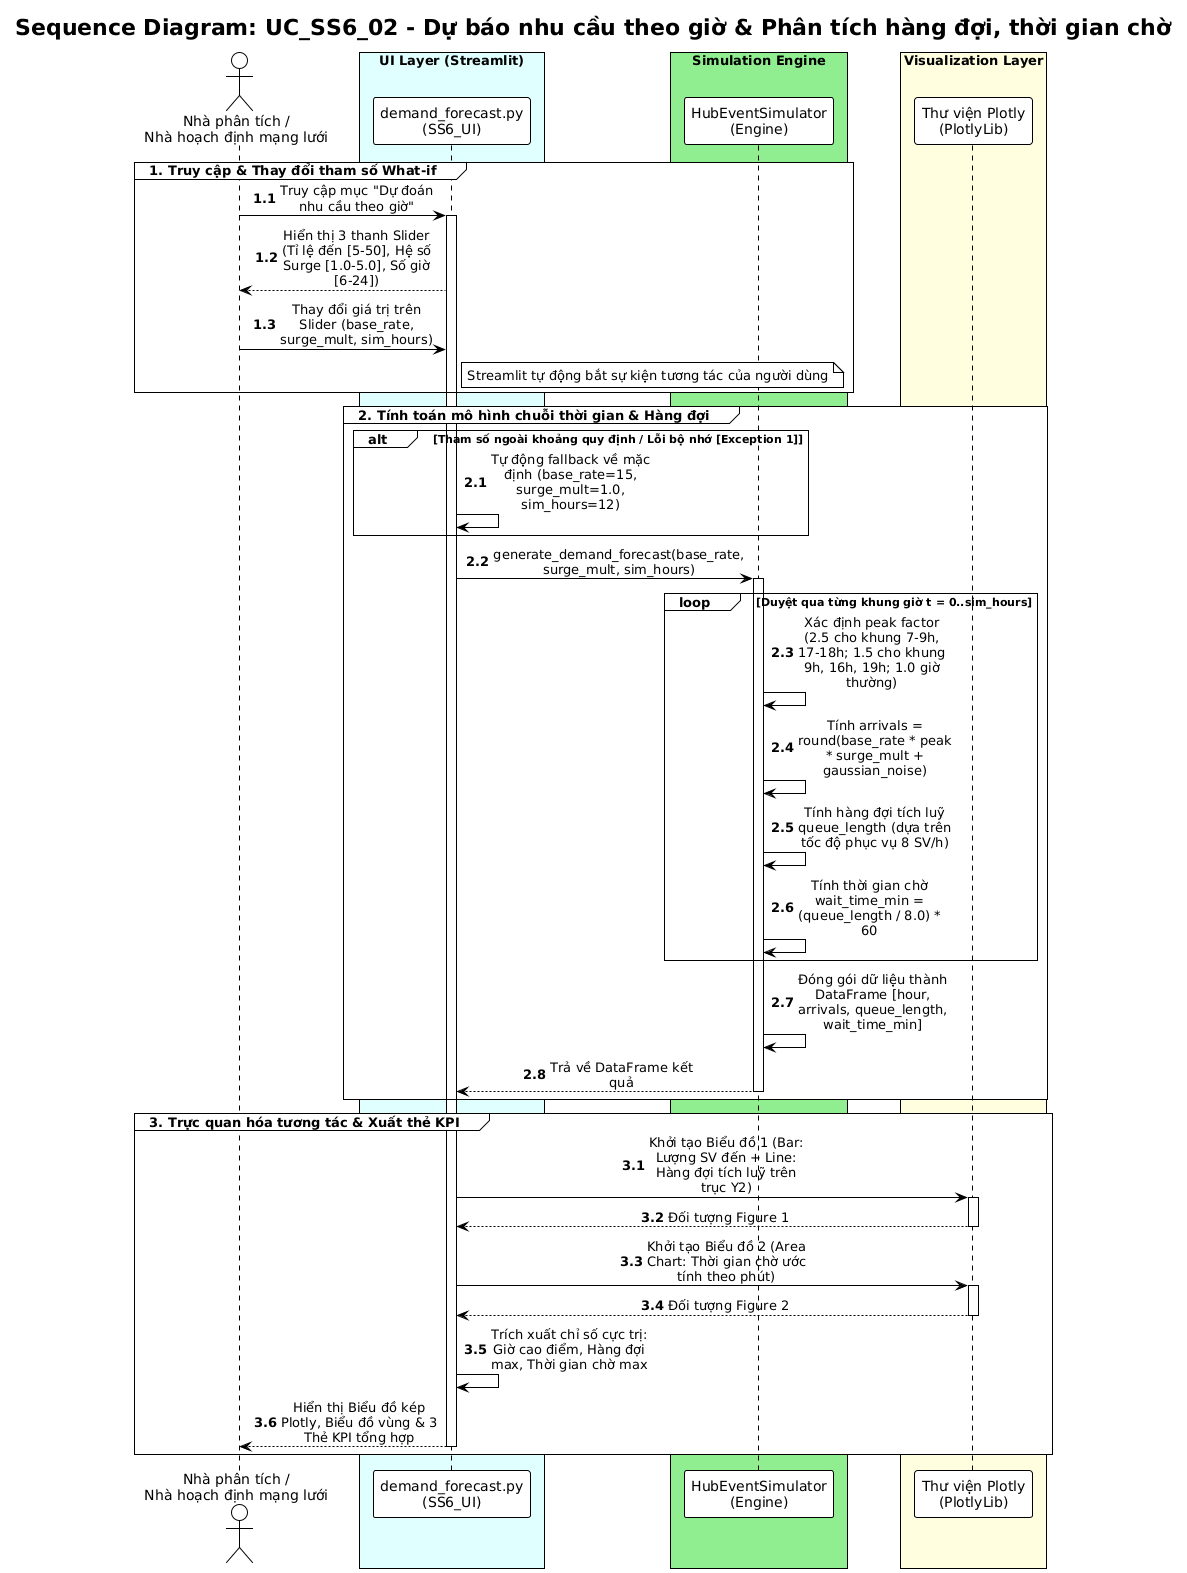
\includegraphics[width=0.88\textwidth,height=0.68\textheight,keepaspectratio]{Use-case detail-scenario/SS6/Sequence diagrams/UC_SS6_02_HoangVanTan_sequence.png}
    \caption{Sơ đồ Tuần tự Chi tiết -- UC\_SS6\_02 (Dự báo nhu cầu theo giờ \& Phân tích hàng đợi)}
    \label{fig:seq-ss6-02}
\end{figure}

% ------------------------------------------------------------
% 2.7 SS7 - Nguyễn Trung Nguyên
% ------------------------------------------------------------
\subsection{Phân hệ SS7: Mô phỏng What-if Hạ tầng (Nguyễn Trung Nguyên)}

\subsubsection{UC\_SS7\_01: Mô phỏng sự cố mất điện / lỗi cổng sạc}
\paragraph{Mô tả nghiệp vụ:} Kỹ thuật viên kích hoạt giả lập mất điện lưới tại Hub, hệ thống tự động cách ly các trụ sạc, chuyển sang nguồn UPS dự phòng cho cảm biến và cảnh báo dừng tiếp nhận đặt chỗ.
\begin{figure}[H]
    \centering
    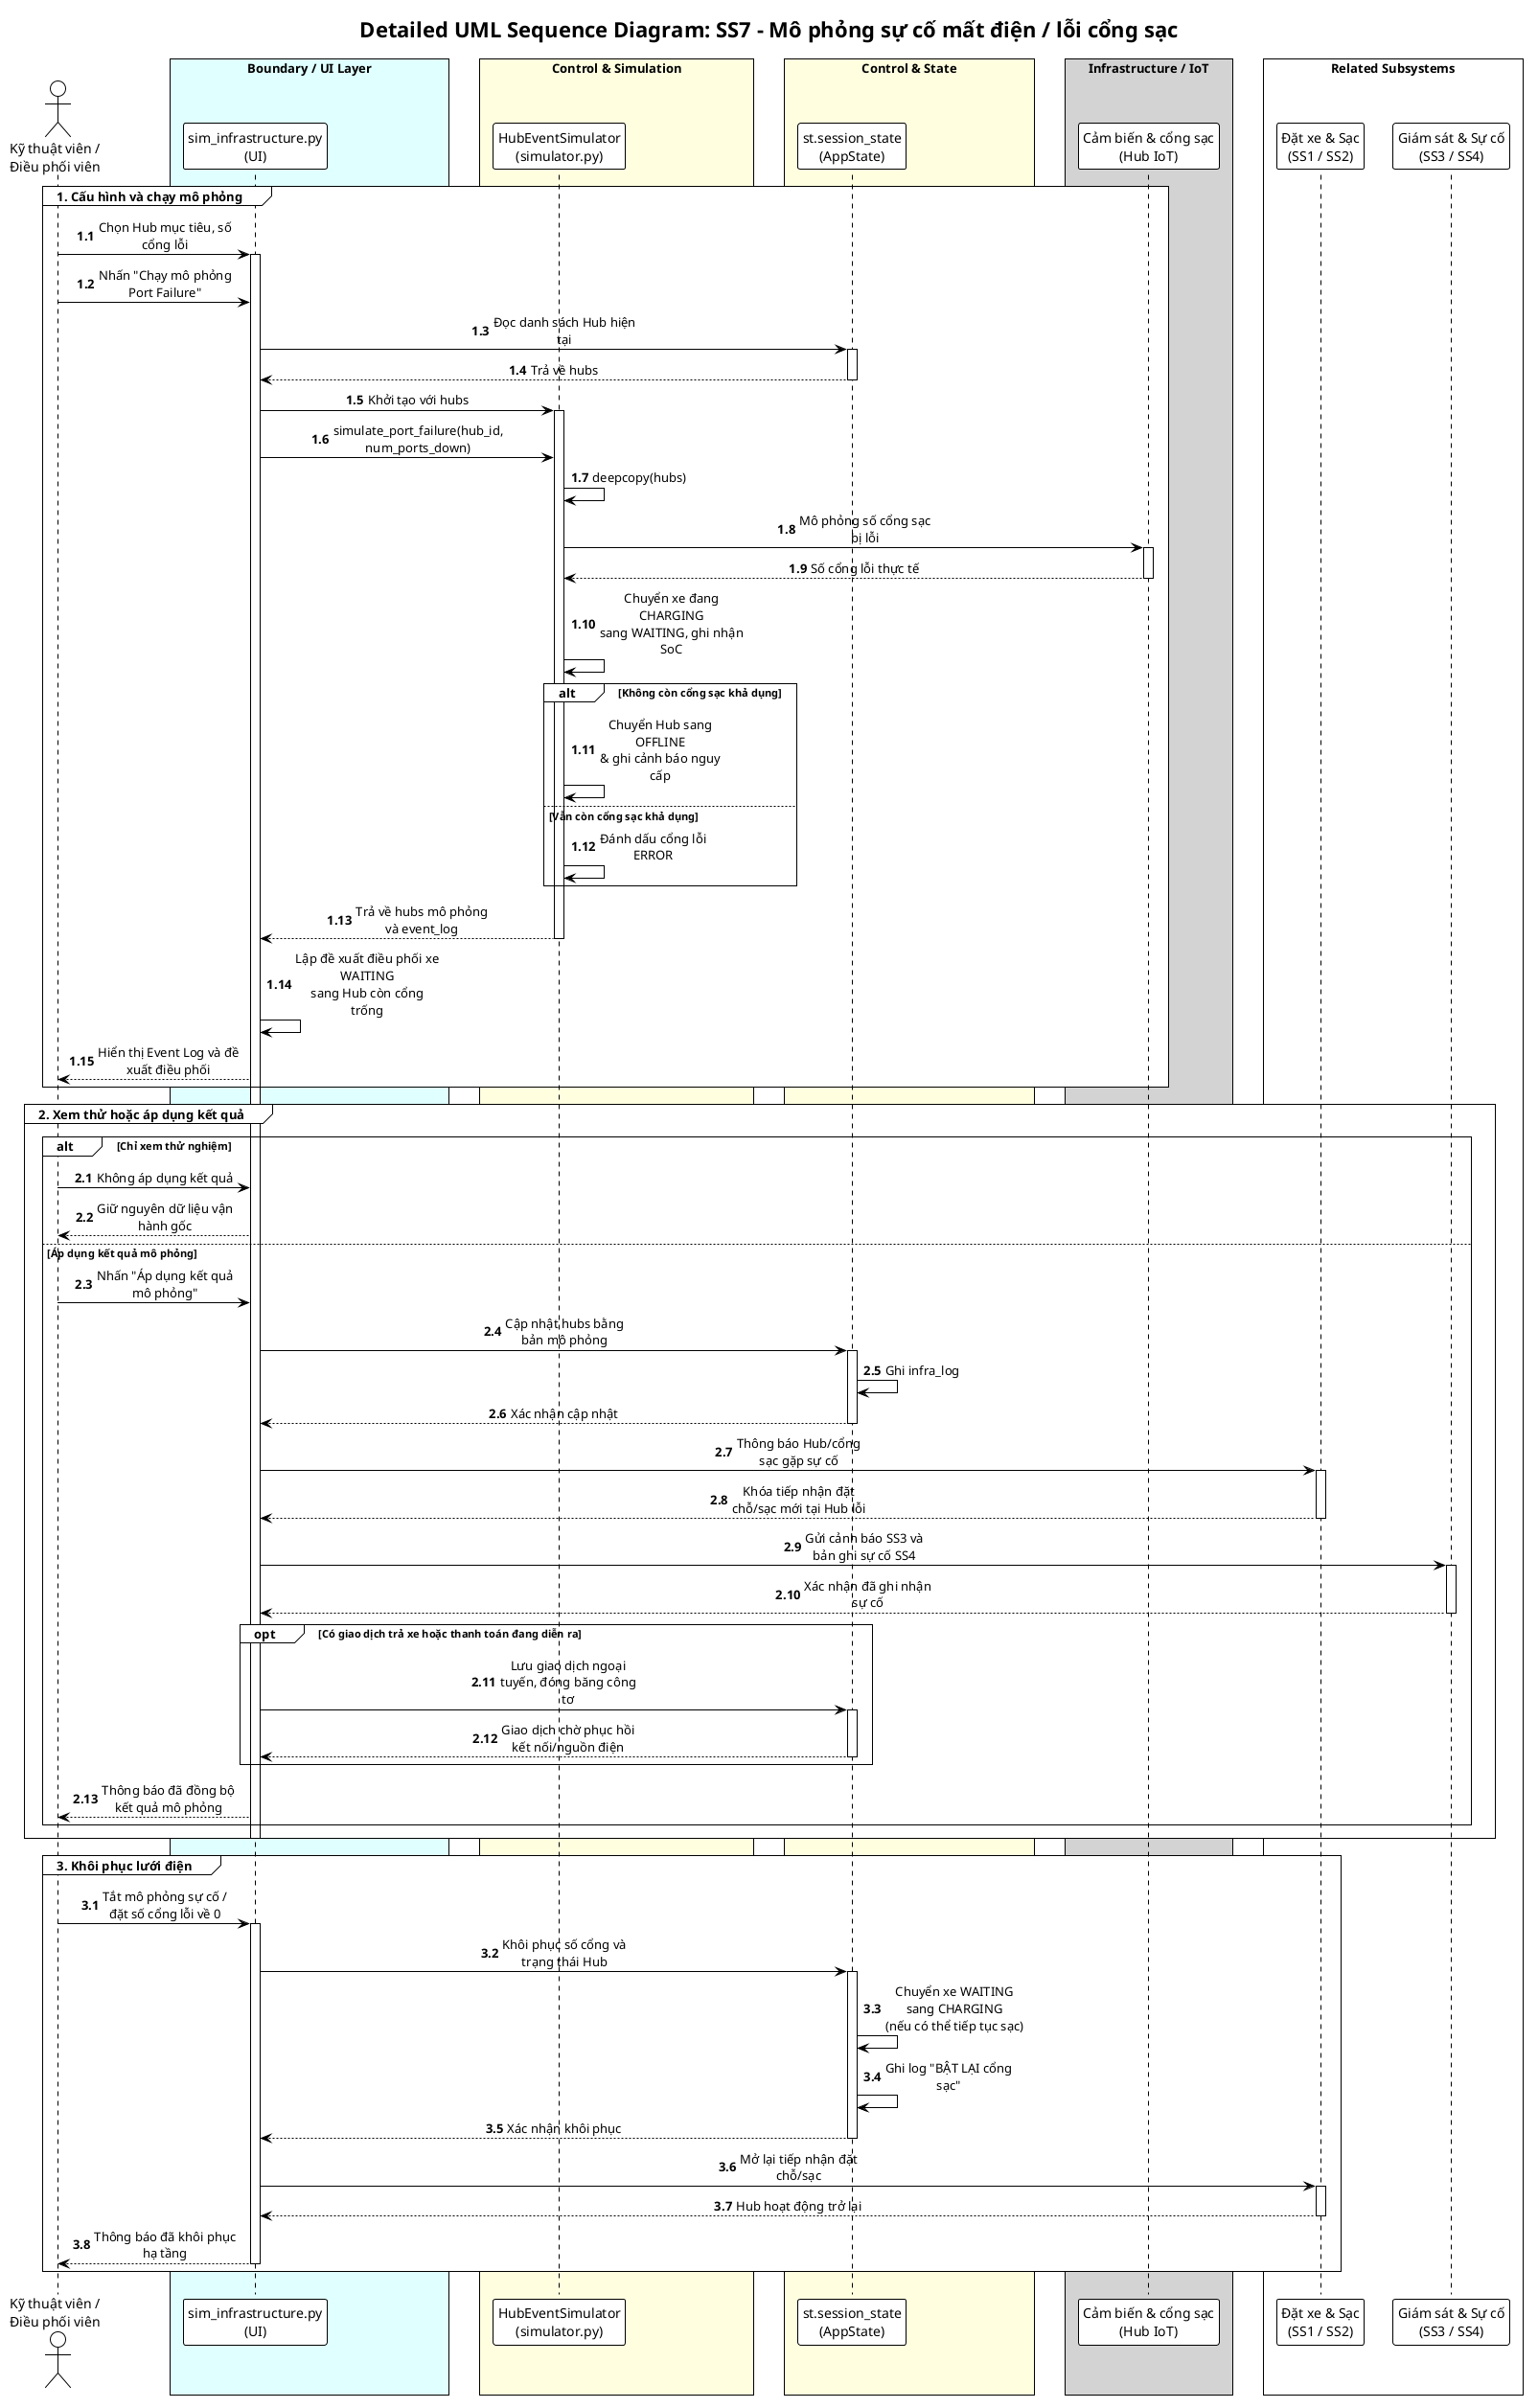
\includegraphics[width=0.88\textwidth,height=0.68\textheight,keepaspectratio]{Use-case detail-scenario/SS7/Sequence diagrams/UC_SS7_01_NguyenTrungNguyen_sequence.png}
    \caption{Sơ đồ Tuần tự Chi tiết -- UC\_SS7\_01 (Mô phỏng sự cố mất điện / lỗi trụ sạc)}
    \label{fig:seq-ss7-01}
\end{figure}

\subsubsection{UC\_SS7\_02: Tự động phát cảnh báo \& Gợi ý điều hướng 1-chạm}
\paragraph{Mô tả nghiệp vụ:} Quét ma trận khoảng cách không gian (Spatial Matrix), tìm 02 Hub lân cận còn slot trống, gửi thông báo điều hướng 1-chạm (One-tap Rerouting) đến sinh viên kèm ưu đãi miễn phí thêm 15 phút.
\begin{figure}[H]
    \centering
    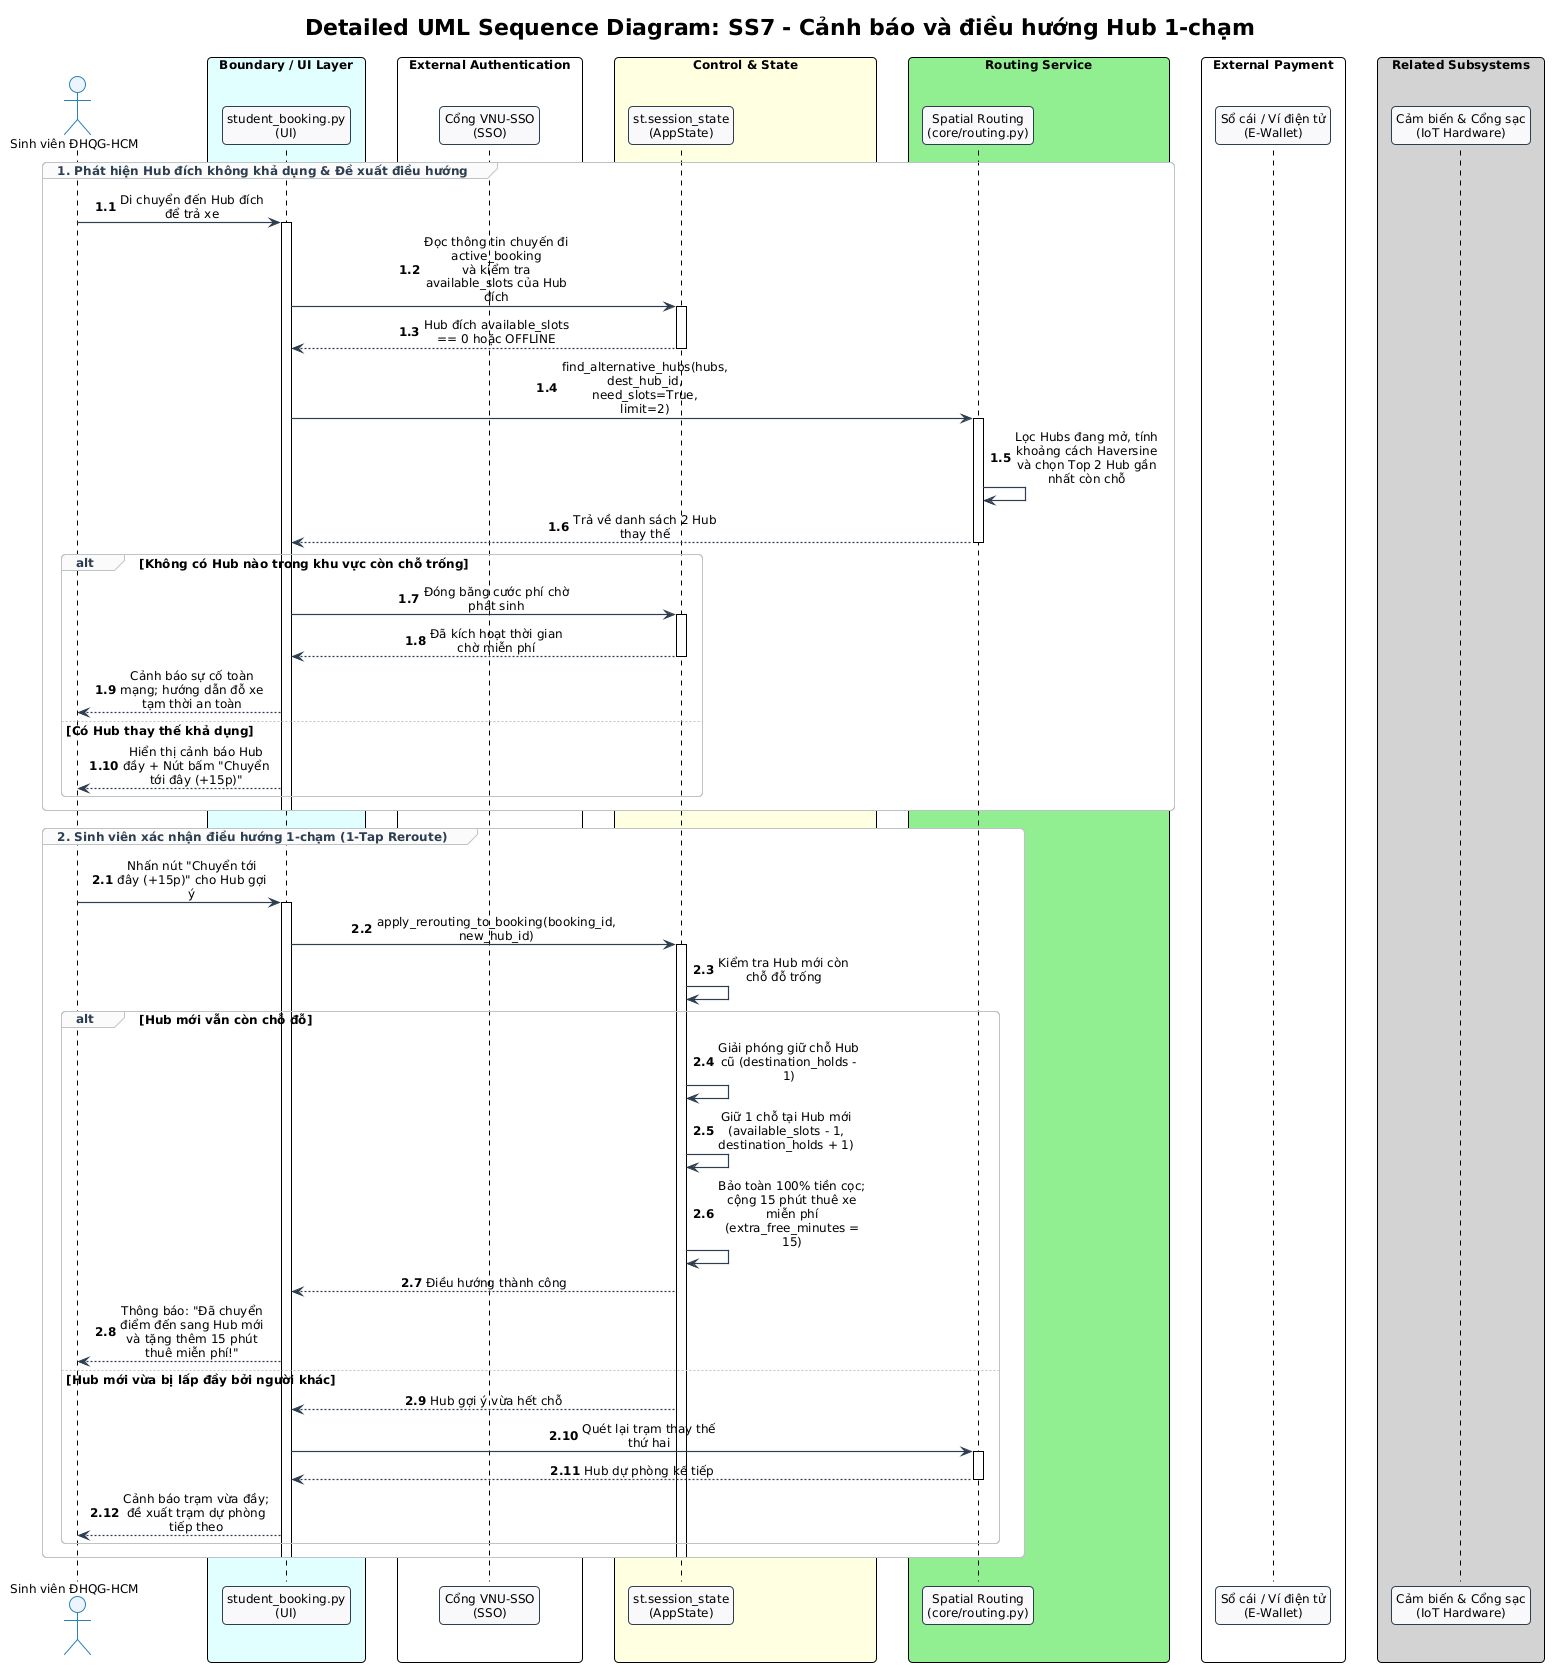
\includegraphics[width=0.88\textwidth,height=0.68\textheight,keepaspectratio]{Use-case detail-scenario/SS7/Sequence diagrams/UC_SS7_02_NguyenTrungNguyen_sequence.png}
    \caption{Sơ đồ Tuần tự Chi tiết -- UC\_SS7\_02 (Tự động phát cảnh báo \& Điều hướng 1-chạm)}
    \label{fig:seq-ss7-02}
\end{figure}
\newpage

% ============================================================
%       MỤC 3: SƠ ĐỒ HOẠT ĐỘNG - ACTIVITY DIAGRAMS (INDIVIDUAL WORK)
% ============================================================
\section{Sơ đồ Hoạt động -- Activity Diagrams (Individual Work)}

Sơ đồ hoạt động (Activity Diagram) thể hiện luồng điều khiển của quy trình nghiệp vụ với các làn bơi (\textbf{Swimlanes}) phân chia rõ ràng giữa \textbf{Người dùng (User / Actor)} và \textbf{Hệ thống (System / IoT / Backend)}.

\subsection*{Nguyên tắc Chuẩn hóa Luồng Nghiệp vụ (Alternative vs. Exception Flows)}
Toàn bộ 17 sơ đồ hoạt động phân làn (Swimlane Activity Diagrams) tuân thủ triệt để nguyên tắc phân định luồng rẽ nhánh:
\begin{itemize}[nosep]
    \item \textbf{Luồng Rẽ nhánh Nghiệp vụ (Alternative Flow):} Được biểu diễn qua các nút quyết định (\texttt{Decision Node}) với điều kiện bảo vệ (\texttt{Guard Condition}). Đây là các kịch bản nghiệp vụ hợp lệ có thể xảy ra trong thực tế (vd: số dư ví không đủ $\rightarrow$ gợi ý nạp tiền; hết xe khả dụng $\rightarrow$ đề xuất trạm lân cận; hết 15 phút ân hạn $\rightarrow$ áp dụng phí phạt giữ chỗ). Hệ thống luôn kiểm soát và điều hướng an toàn để kết thúc phiên.
    \item \textbf{Luồng Xử lý Ngoại lệ Kỹ thuật (Exception Flow):} Được bao bọc trong vùng ngắt có thể gián đoạn (\texttt{Interruptible Activity Region}) dẫn tới nút hủy (\texttt{Flow Final} hoặc \texttt{Activity Final}). Luồng này chỉ kích hoạt khi xảy ra sự cố kỹ thuật bất thường ngoài tầm kiểm soát nghiệp vụ (vd: mất kết nối internet/CSDL, cổng sạc quá nhiệt ngắt mạch, mất điện lưới diện rộng).
\end{itemize}

\begin{table}[H]
    \centering
    \small
    \renewcommand{\arraystretch}{1.2}
    \caption{Ma trận Phân loại Luồng Nghiệp vụ trong 17 Activity Diagrams}
    \label{tab:act-matrix}
    \begin{tabularx}{\textwidth}{|c|c|X|X|}
        \hline
        \textbf{Phân hệ} & \textbf{Mã UC} & \textbf{Luồng Rẽ Nhánh (Alternate Flow)} & \textbf{Luồng Ngoại Lệ (Exception Flow)} \\
        \hline
        SS1 & UC\_SS1\_01 & Nhập mã PIN thủ công thay vì quét QR & Số dư ví không đủ 50.000 VNĐ; quá 15p No-show (phạt 10k, hoàn 40k) \\
        SS1 & UC\_SS1\_02 & Trả xe tại Hub khác điểm mượn & Hub đích đầy/offline: kích hoạt gợi ý 1-chạm sang Hub lân cận \\
        SS1 & UC\_SS1\_03 & Hủy trong 15p hoàn 100\% cọc; chọn tìm Hub khác & Quá 15p không nhận (No-show: phạt 10k, hoàn 40k) \\
        \hline
        SS2 & UC\_SS2\_01 & Bổ sung giấy tờ xe qua xác minh thủ công & Biển số xe đã tồn tại trên hệ thống \\
        SS2 & UC\_SS2\_02 & Chỉ đỗ xe không sạc điện & Hết chỗ đỗ hoặc không có cổng sạc phù hợp \\
        SS2 & UC\_SS2\_03 & Nhận diện tự động qua camera ANPR & Thẻ RFID lỗi, nhập mã đặt chỗ dự phòng \\
        SS2 & UC\_SS2\_04 & Thanh toán qua ví điện tử nội bộ & Số dư ví không đủ, chuyển cổng VNPay \\
        \hline
        SS3 & UC\_SS3\_01 & Đẩy thông báo lỗi cảm biến sang KTV & Cảm biến IoT timeout, chuyển hiển thị dữ liệu cache \\
        SS3 & UC\_SS3\_02 & Hệ thống tự động đẩy đề xuất lệnh sang SS4 & Người điều hành từ chối lệnh đề xuất \\
        \hline
        SS4 & UC\_SS4\_01 & Điều phối xe tải lớn vận chuyển hàng loạt & Lái xe điều phối báo tắc đường trễ giờ \\
        SS4 & UC\_SS4\_02 & Kỹ thuật viên sửa chữa tại chỗ thành công & Xe hư nặng kéo về xưởng bảo trì trung tâm \\
        \hline
        SS5 & UC\_SS5\_01 & Ưu tiên xe pin thấp dưới 20\% sạc trước & Quá tải công suất trạm, giảm dòng sạc an toàn \\
        SS5 & UC\_SS5\_02 & Sinh viên di chuyển xe trong 15p ân hạn & Quá 15p tính phí chiếm dụng 10.000đ/15p \\
        \hline
        SS6 & UC\_SS6\_01 & Điều chỉnh tham số Metro tăng 200\% & Dữ liệu lịch sử tuyến Metro không khả dụng \\
        SS6 & UC\_SS6\_02 & Tùy chỉnh tham số What-if trực quan & Tham số ngoài khoảng: fallback về giá trị mặc định \\
        \hline
        SS7 & UC\_SS7\_01 & Chuyển tải sang máy phát điện phụ trợ & Trạm sạc chập điện ngắt toàn bộ trạm \\
        SS7 & UC\_SS7\_02 & Sinh viên chấp nhận gợi ý Hub lân cận & Sinh viên từ chối, hủy phiên và hoàn cọc \\
        \hline
    \end{tabularx}
\end{table}

\subsection{Phân hệ SS1: Đặt \& Quản lý Xe dùng chung (Nguyễn Thành Đạt)}

\subsubsection{UC\_SS1\_01: Đặt giữ chỗ \& Quét QR/PIN nhận xe}
\paragraph{Phân tích làn bơi (Swimlane):}
\begin{itemize}[nosep]
    \item \textbf{Làn bơi Sinh viên (Actor):} Mở app $\rightarrow$ Chọn Hub \& Xe $\rightarrow$ Xác nhận đặt cọc $\rightarrow$ Quét mã QR/PIN tại Hub.
    \item \textbf{Làn bơi Hệ thống (Backend/IoT):} Kiểm tra ví $\ge 50$k $\rightarrow$ Khóa xe 15p $\rightarrow$ Xác thực mã PIN/QR $\rightarrow$ Mở khóa vật lý $\rightarrow$ Chuyển \texttt{IN\_USE}.
\end{itemize}
\begin{figure}[H]
    \centering
    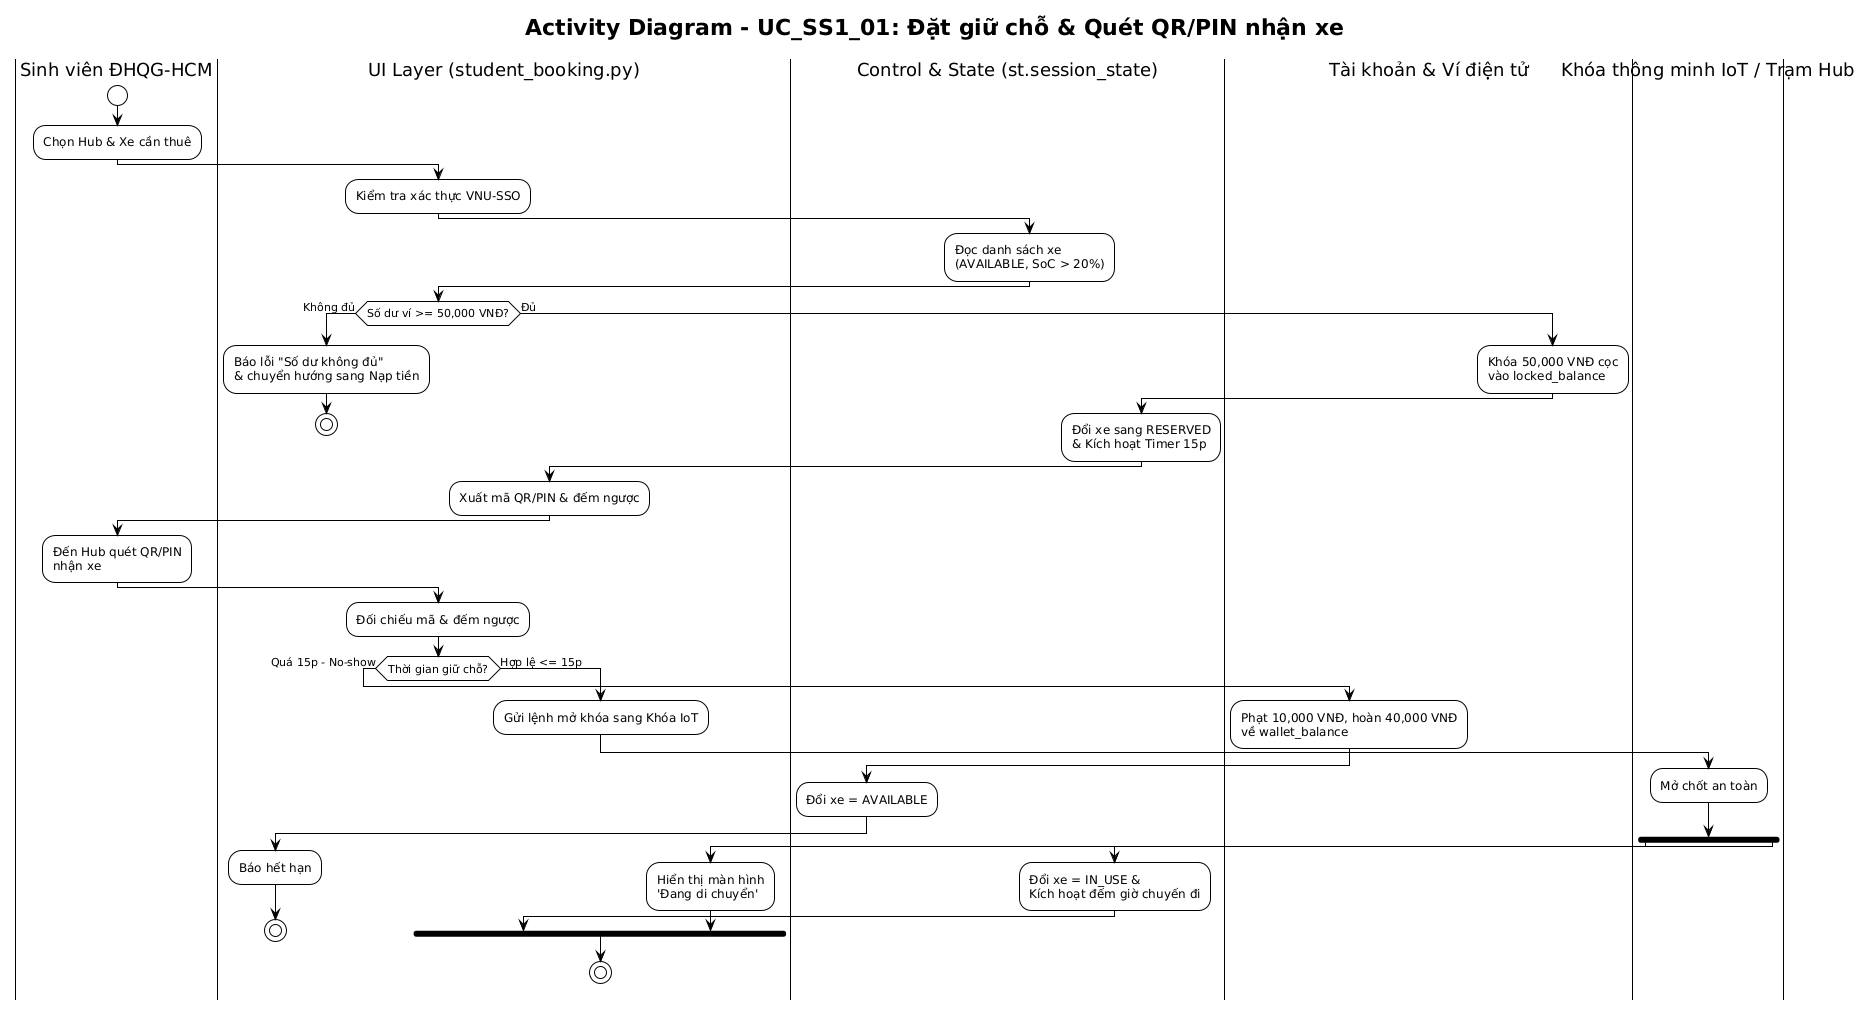
\includegraphics[width=0.92\textwidth,height=0.68\textheight,keepaspectratio]{Use-case detail-scenario/SS1/Activity diagrams/UC_SS1_01_NguyenThanhDat_activity.png}
    \caption{Sơ đồ Hoạt động Phân làn (Swimlane) -- UC\_SS1\_01}
    \label{fig:act-ss1-01}
\end{figure}

\subsubsection{UC\_SS1\_02: Trả xe 1-chiều \& Quyết toán ví điện tử}
\begin{figure}[H]
    \centering
    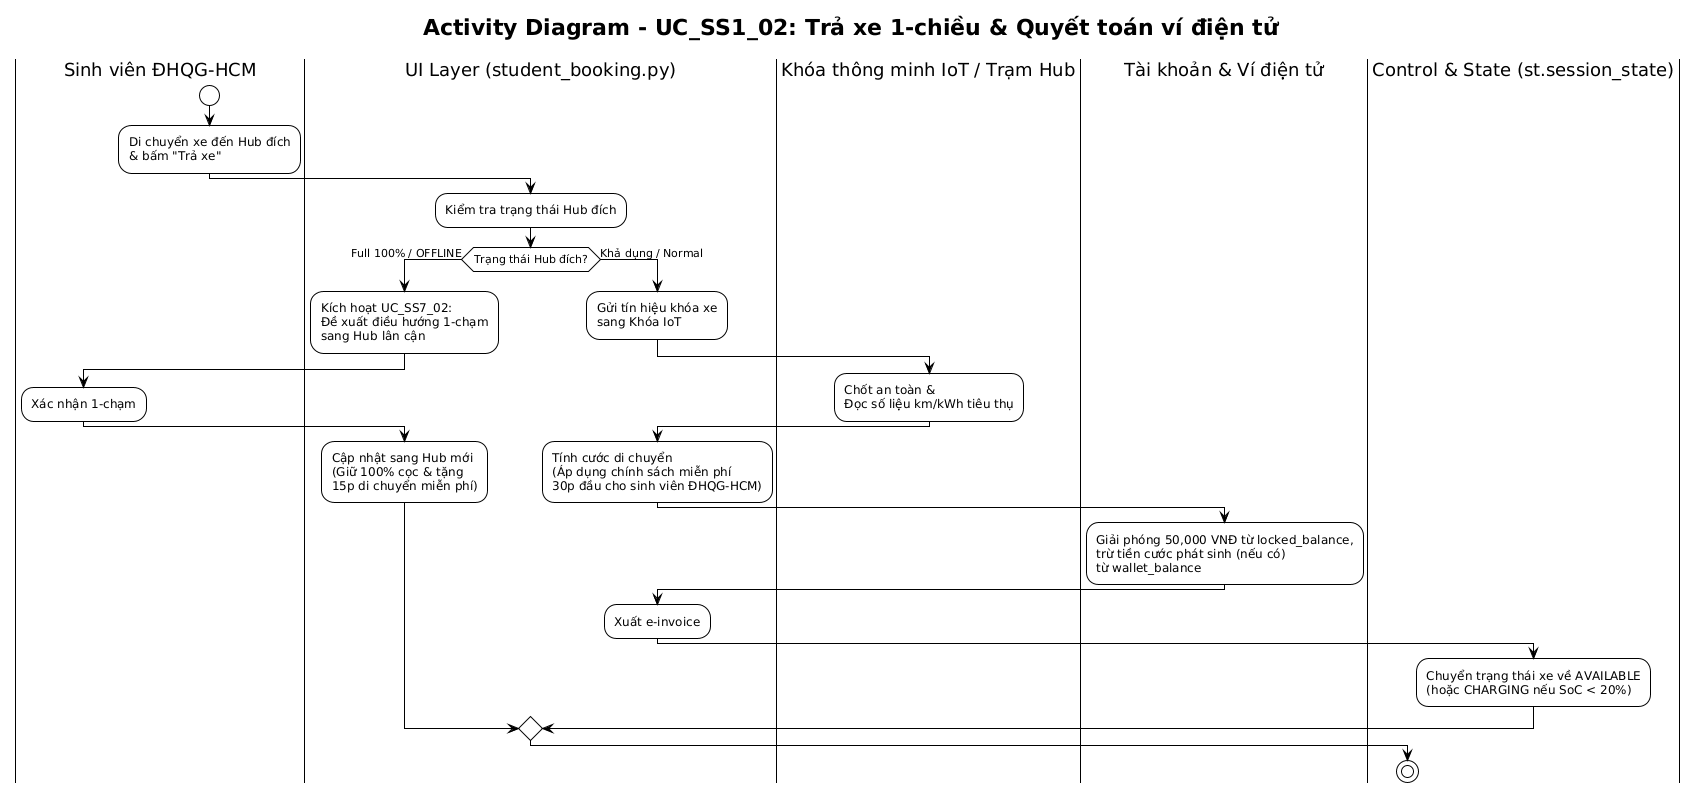
\includegraphics[width=0.92\textwidth,height=0.68\textheight,keepaspectratio]{Use-case detail-scenario/SS1/Activity diagrams/UC_SS1_02_NguyenThanhDat_activity.png}
    \caption{Sơ đồ Hoạt động Phân làn (Swimlane) -- UC\_SS1\_02}
    \label{fig:act-ss1-02}
\end{figure}

\subsubsection{UC\_SS1\_03: Hủy đặt xe \& Hoàn cọc / Phạt No-show}
\begin{figure}[H]
    \centering
    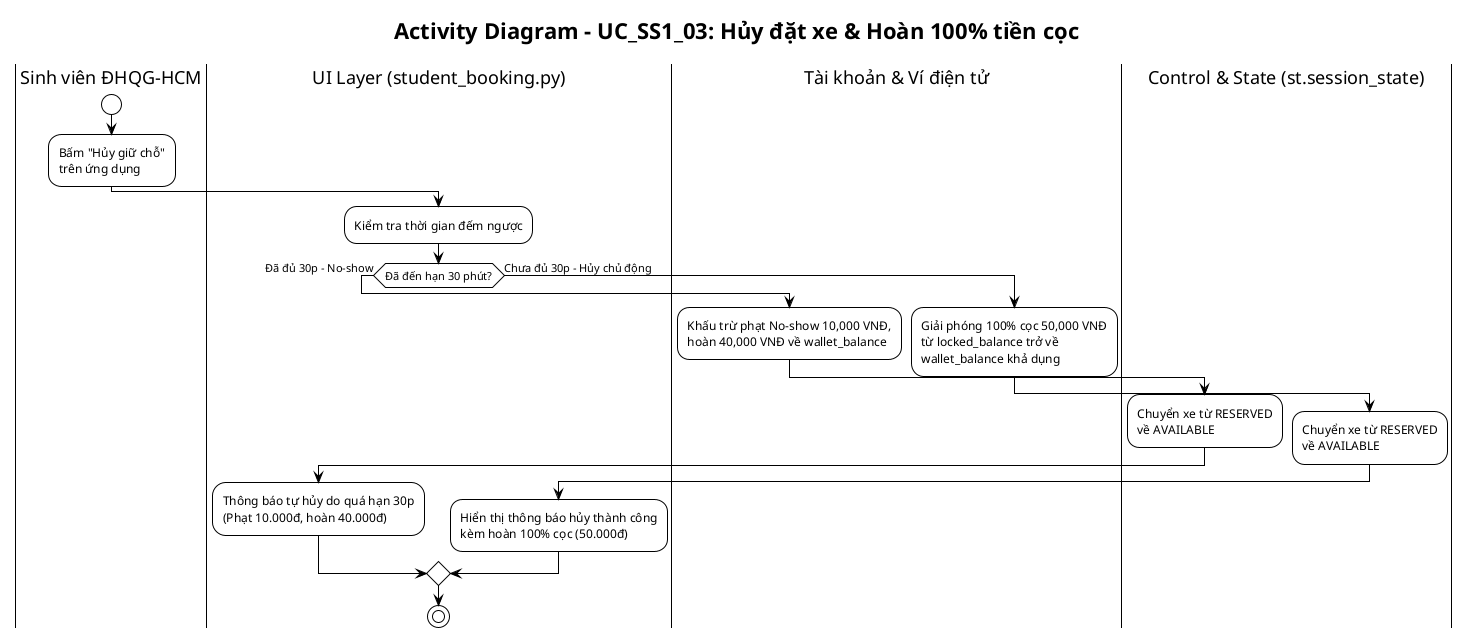
\includegraphics[width=0.92\textwidth,height=0.68\textheight,keepaspectratio]{Use-case detail-scenario/SS1/Activity diagrams/UC_SS1_03_NguyenThanhDat_activity.png}
    \caption{Sơ đồ Hoạt động Phân làn (Swimlane) -- UC\_SS1\_03 (Hủy đặt xe \& Hoàn cọc / Phạt No-show)}
    \label{fig:act-ss1-03}
\end{figure}

\subsection{Phân hệ SS2: Đăng ký Sạc \& Đỗ xe cá nhân (Nguyễn Anh Tài)}
\subsubsection{UC\_SS2\_01: Đăng ký xe EV cá nhân}
\begin{figure}[H]
    \centering
    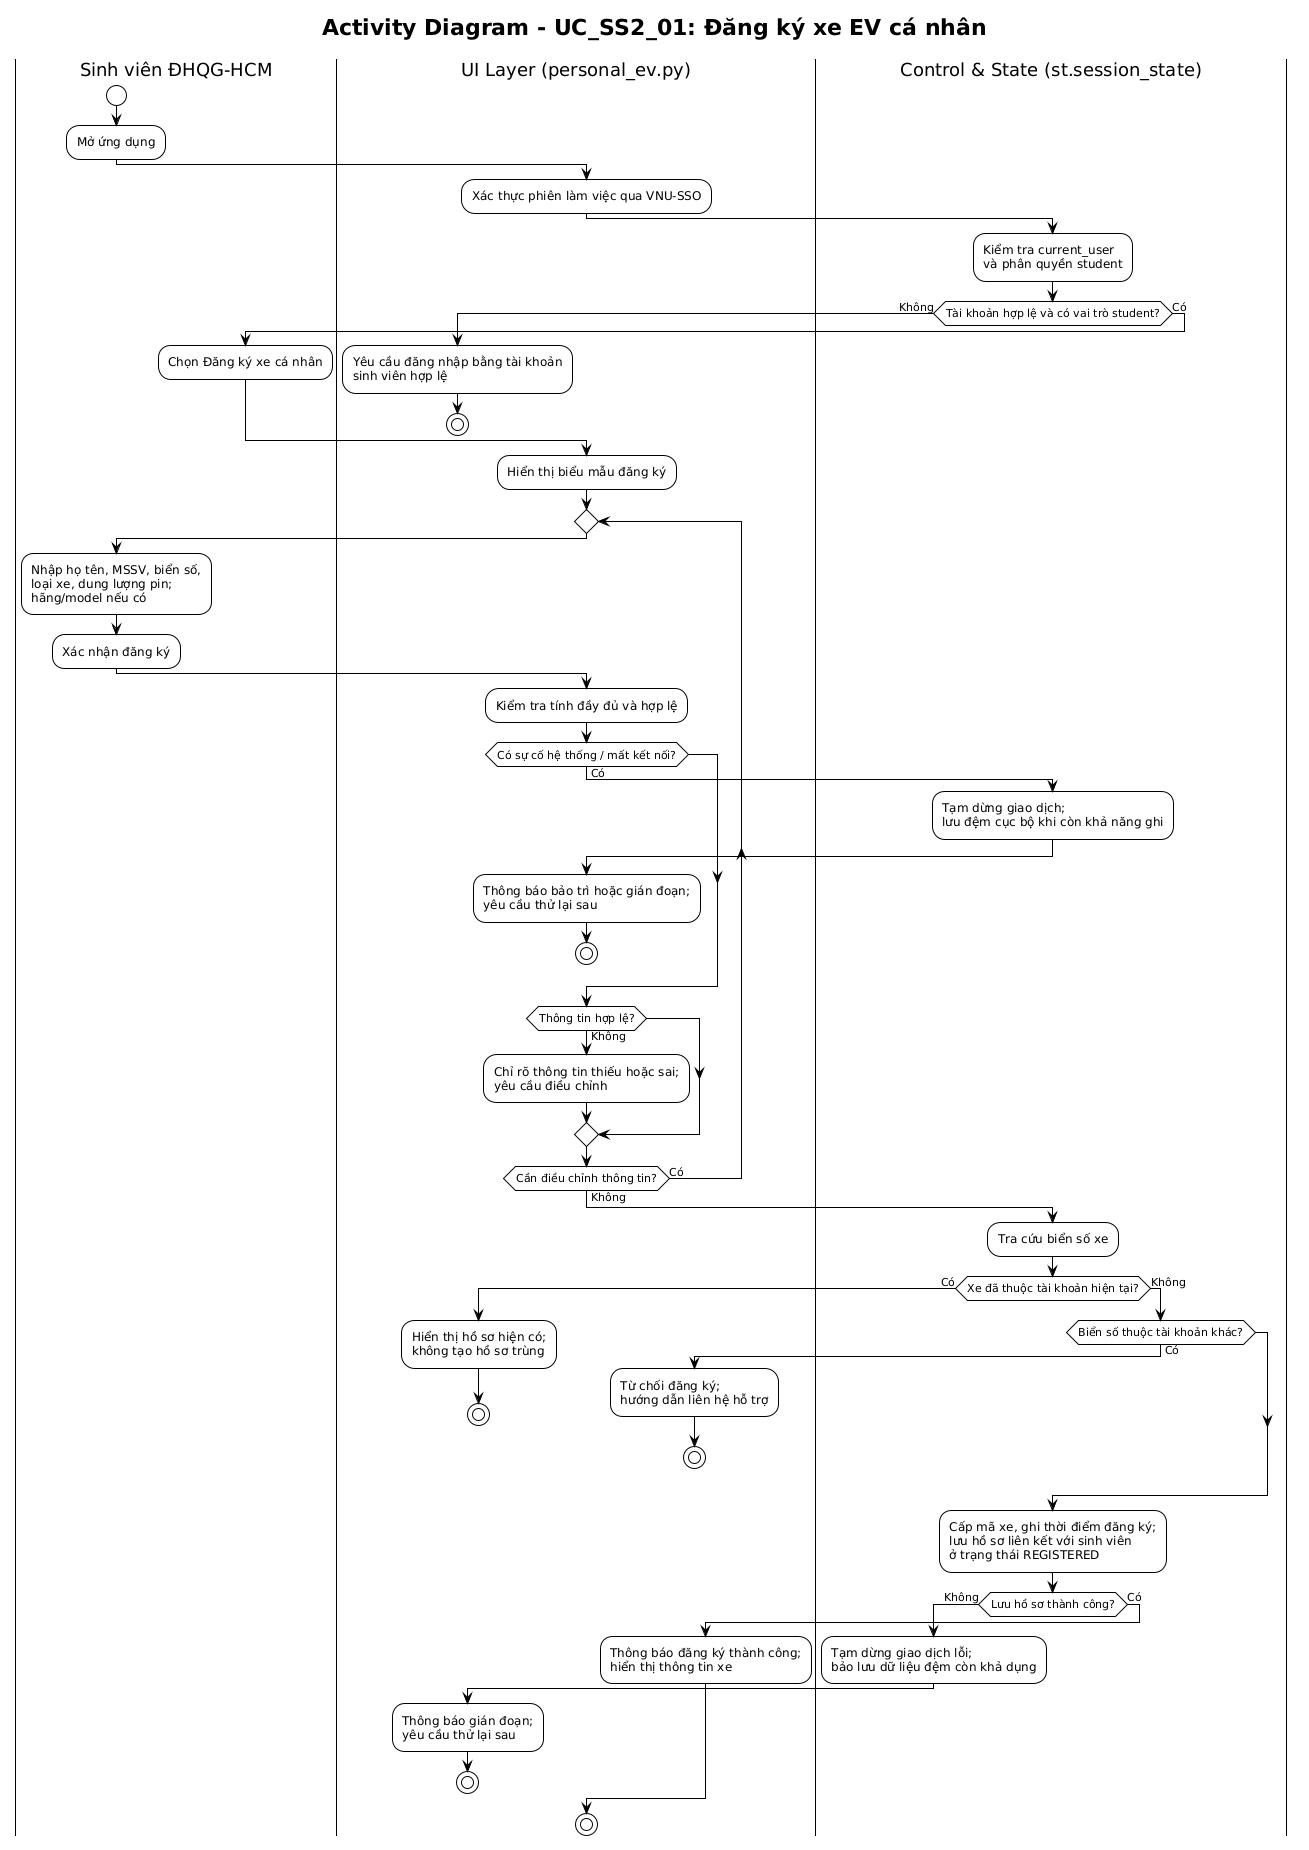
\includegraphics[width=0.92\textwidth,height=0.68\textheight,keepaspectratio]{Use-case detail-scenario/SS2/Activity diagrams/UC_SS2_01_NguyenAnhTai_activity.png}
    \caption{Sơ đồ Hoạt động Phân làn -- UC\_SS2\_01}
    \label{fig:act-ss2-01}
\end{figure}

\clearpage
\subsubsection{UC\_SS2\_02: Đặt chỗ đỗ và nhu cầu sạc xe EV cá nhân}
\begin{figure}[H]
    \centering
    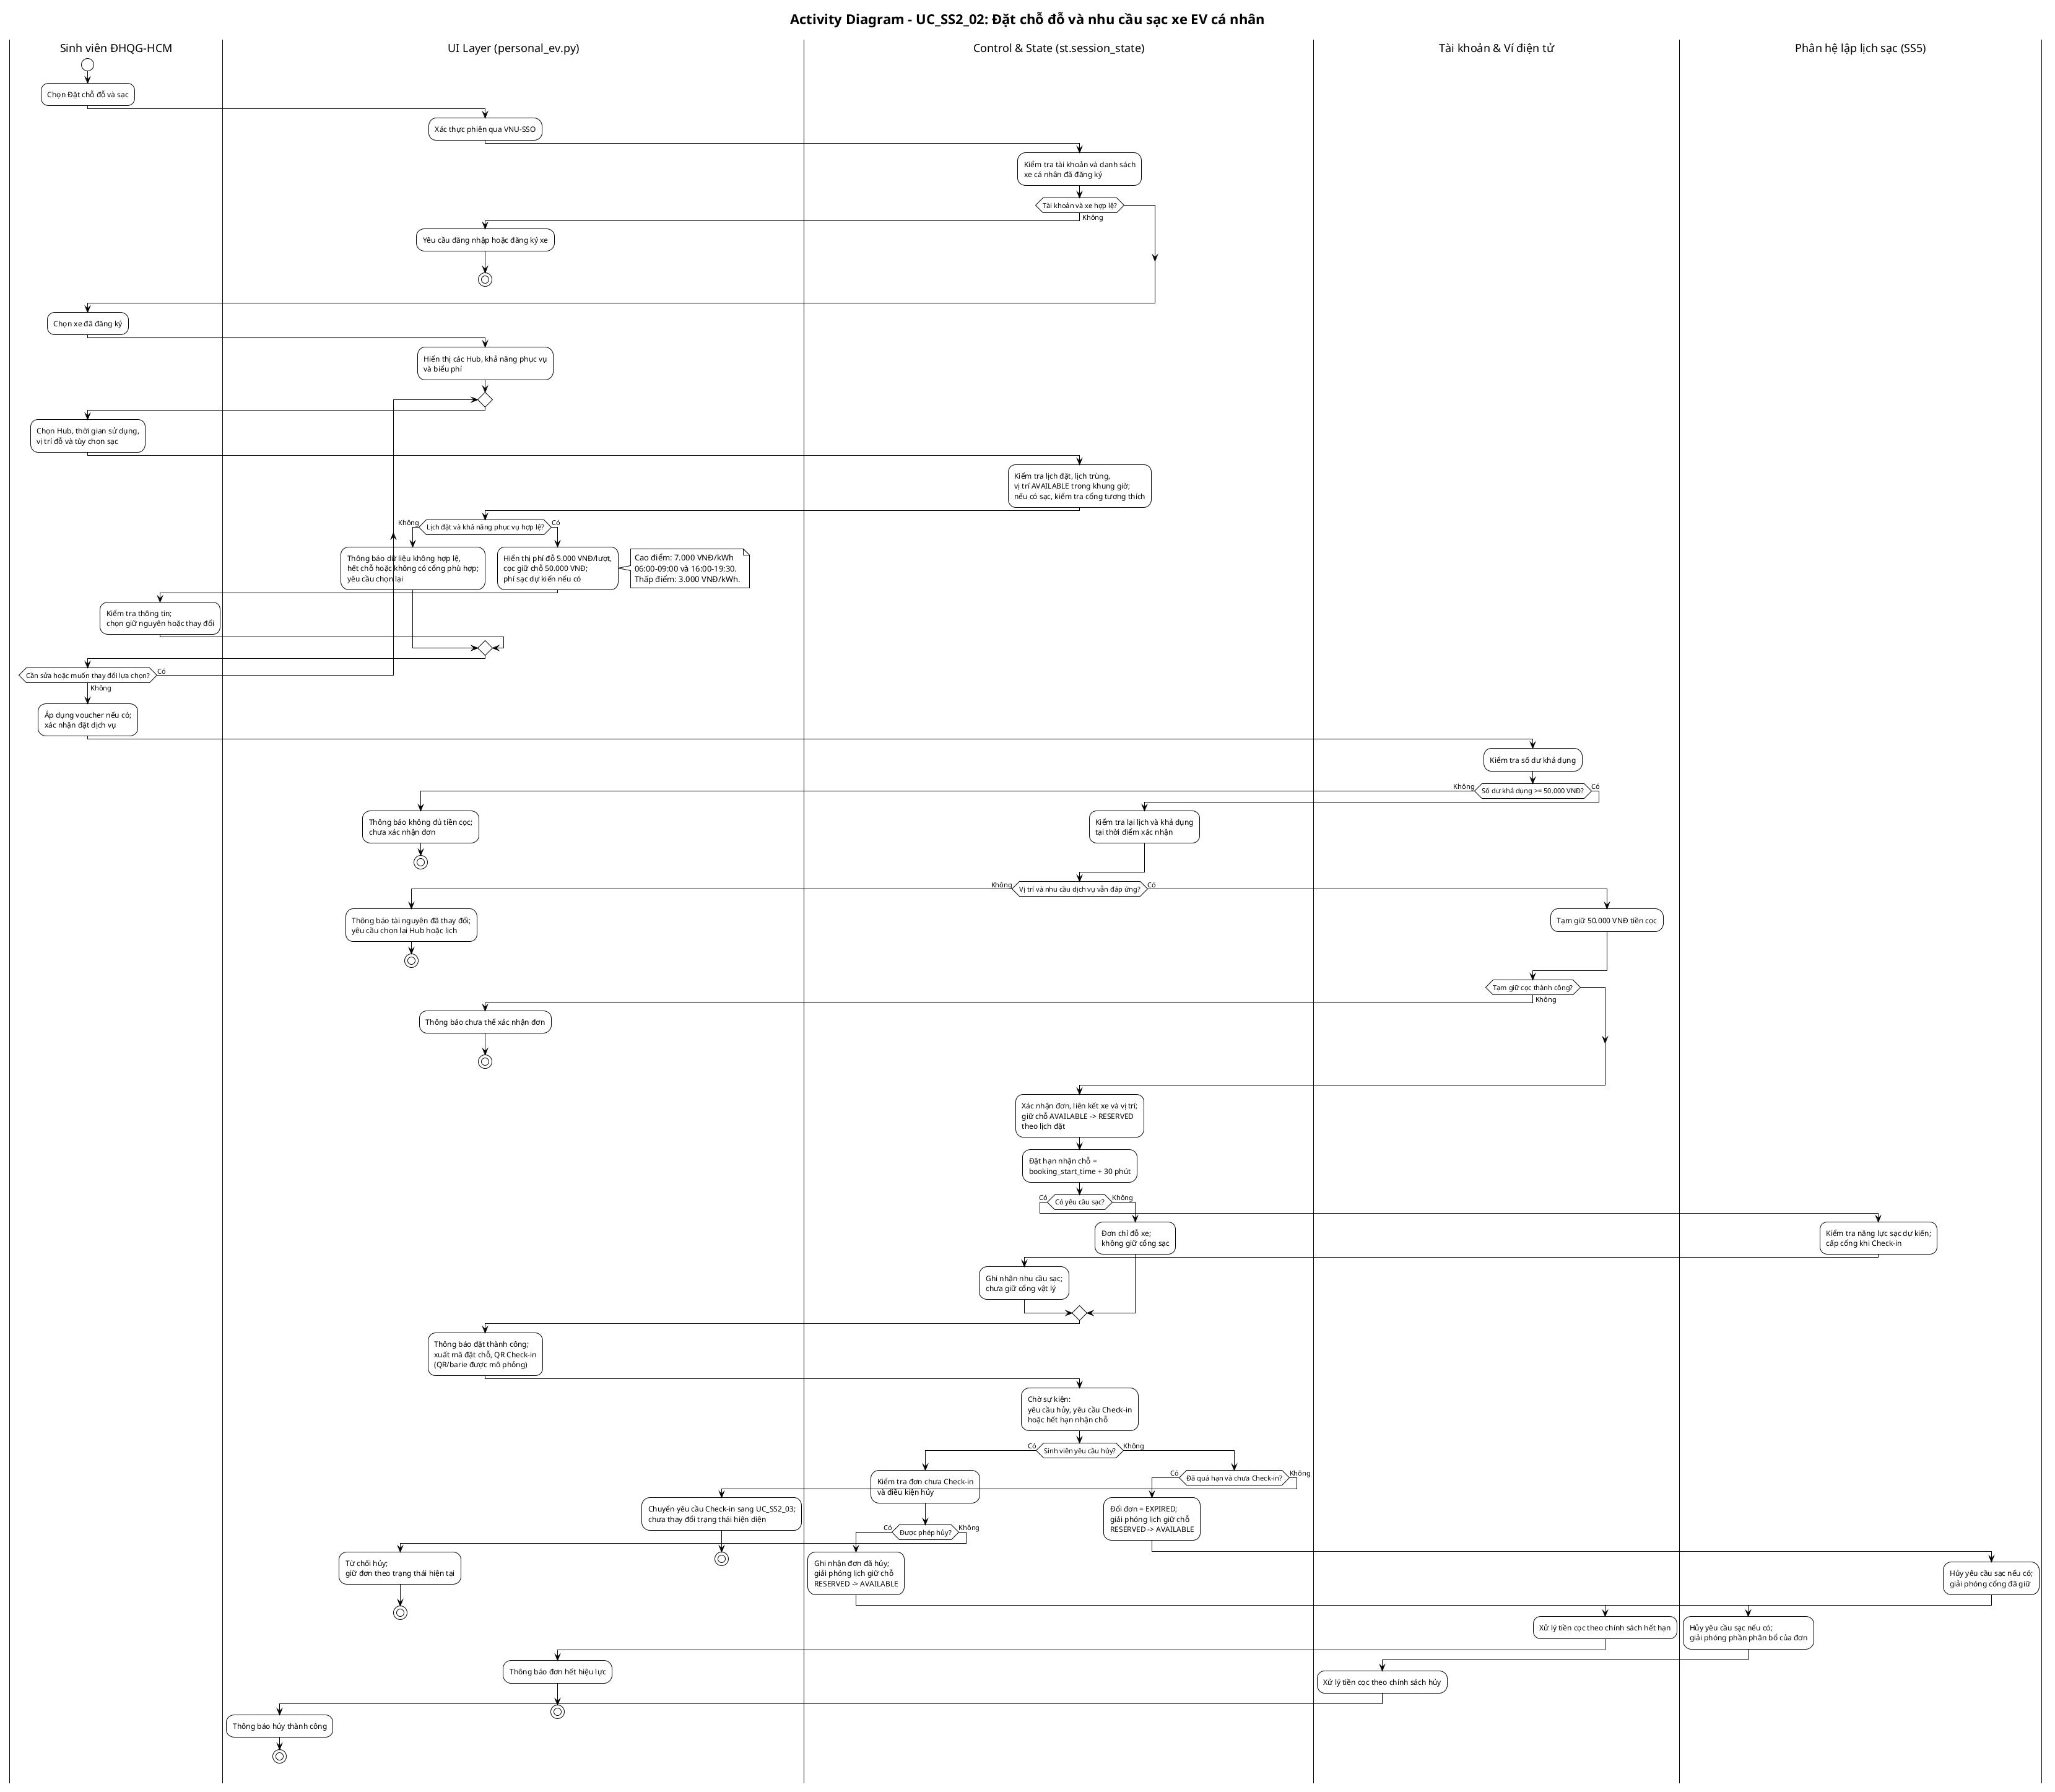
\includegraphics[width=0.92\textwidth,height=0.70\textheight,keepaspectratio]{Use-case detail-scenario/SS2/Activity diagrams/UC_SS2_02_NguyenAnhTai_activity.png}
    \caption{Sơ đồ Hoạt động Phân làn (Swimlane) -- UC\_SS2\_02 (Đặt chỗ đỗ \& Lịch sạc xe cá nhân)}
    \label{fig:act-ss2-02}
\end{figure}
\clearpage

\subsubsection{UC\_SS2\_03: Check-in xe EV cá nhân tại Hub}
\begin{figure}[H]
    \centering
    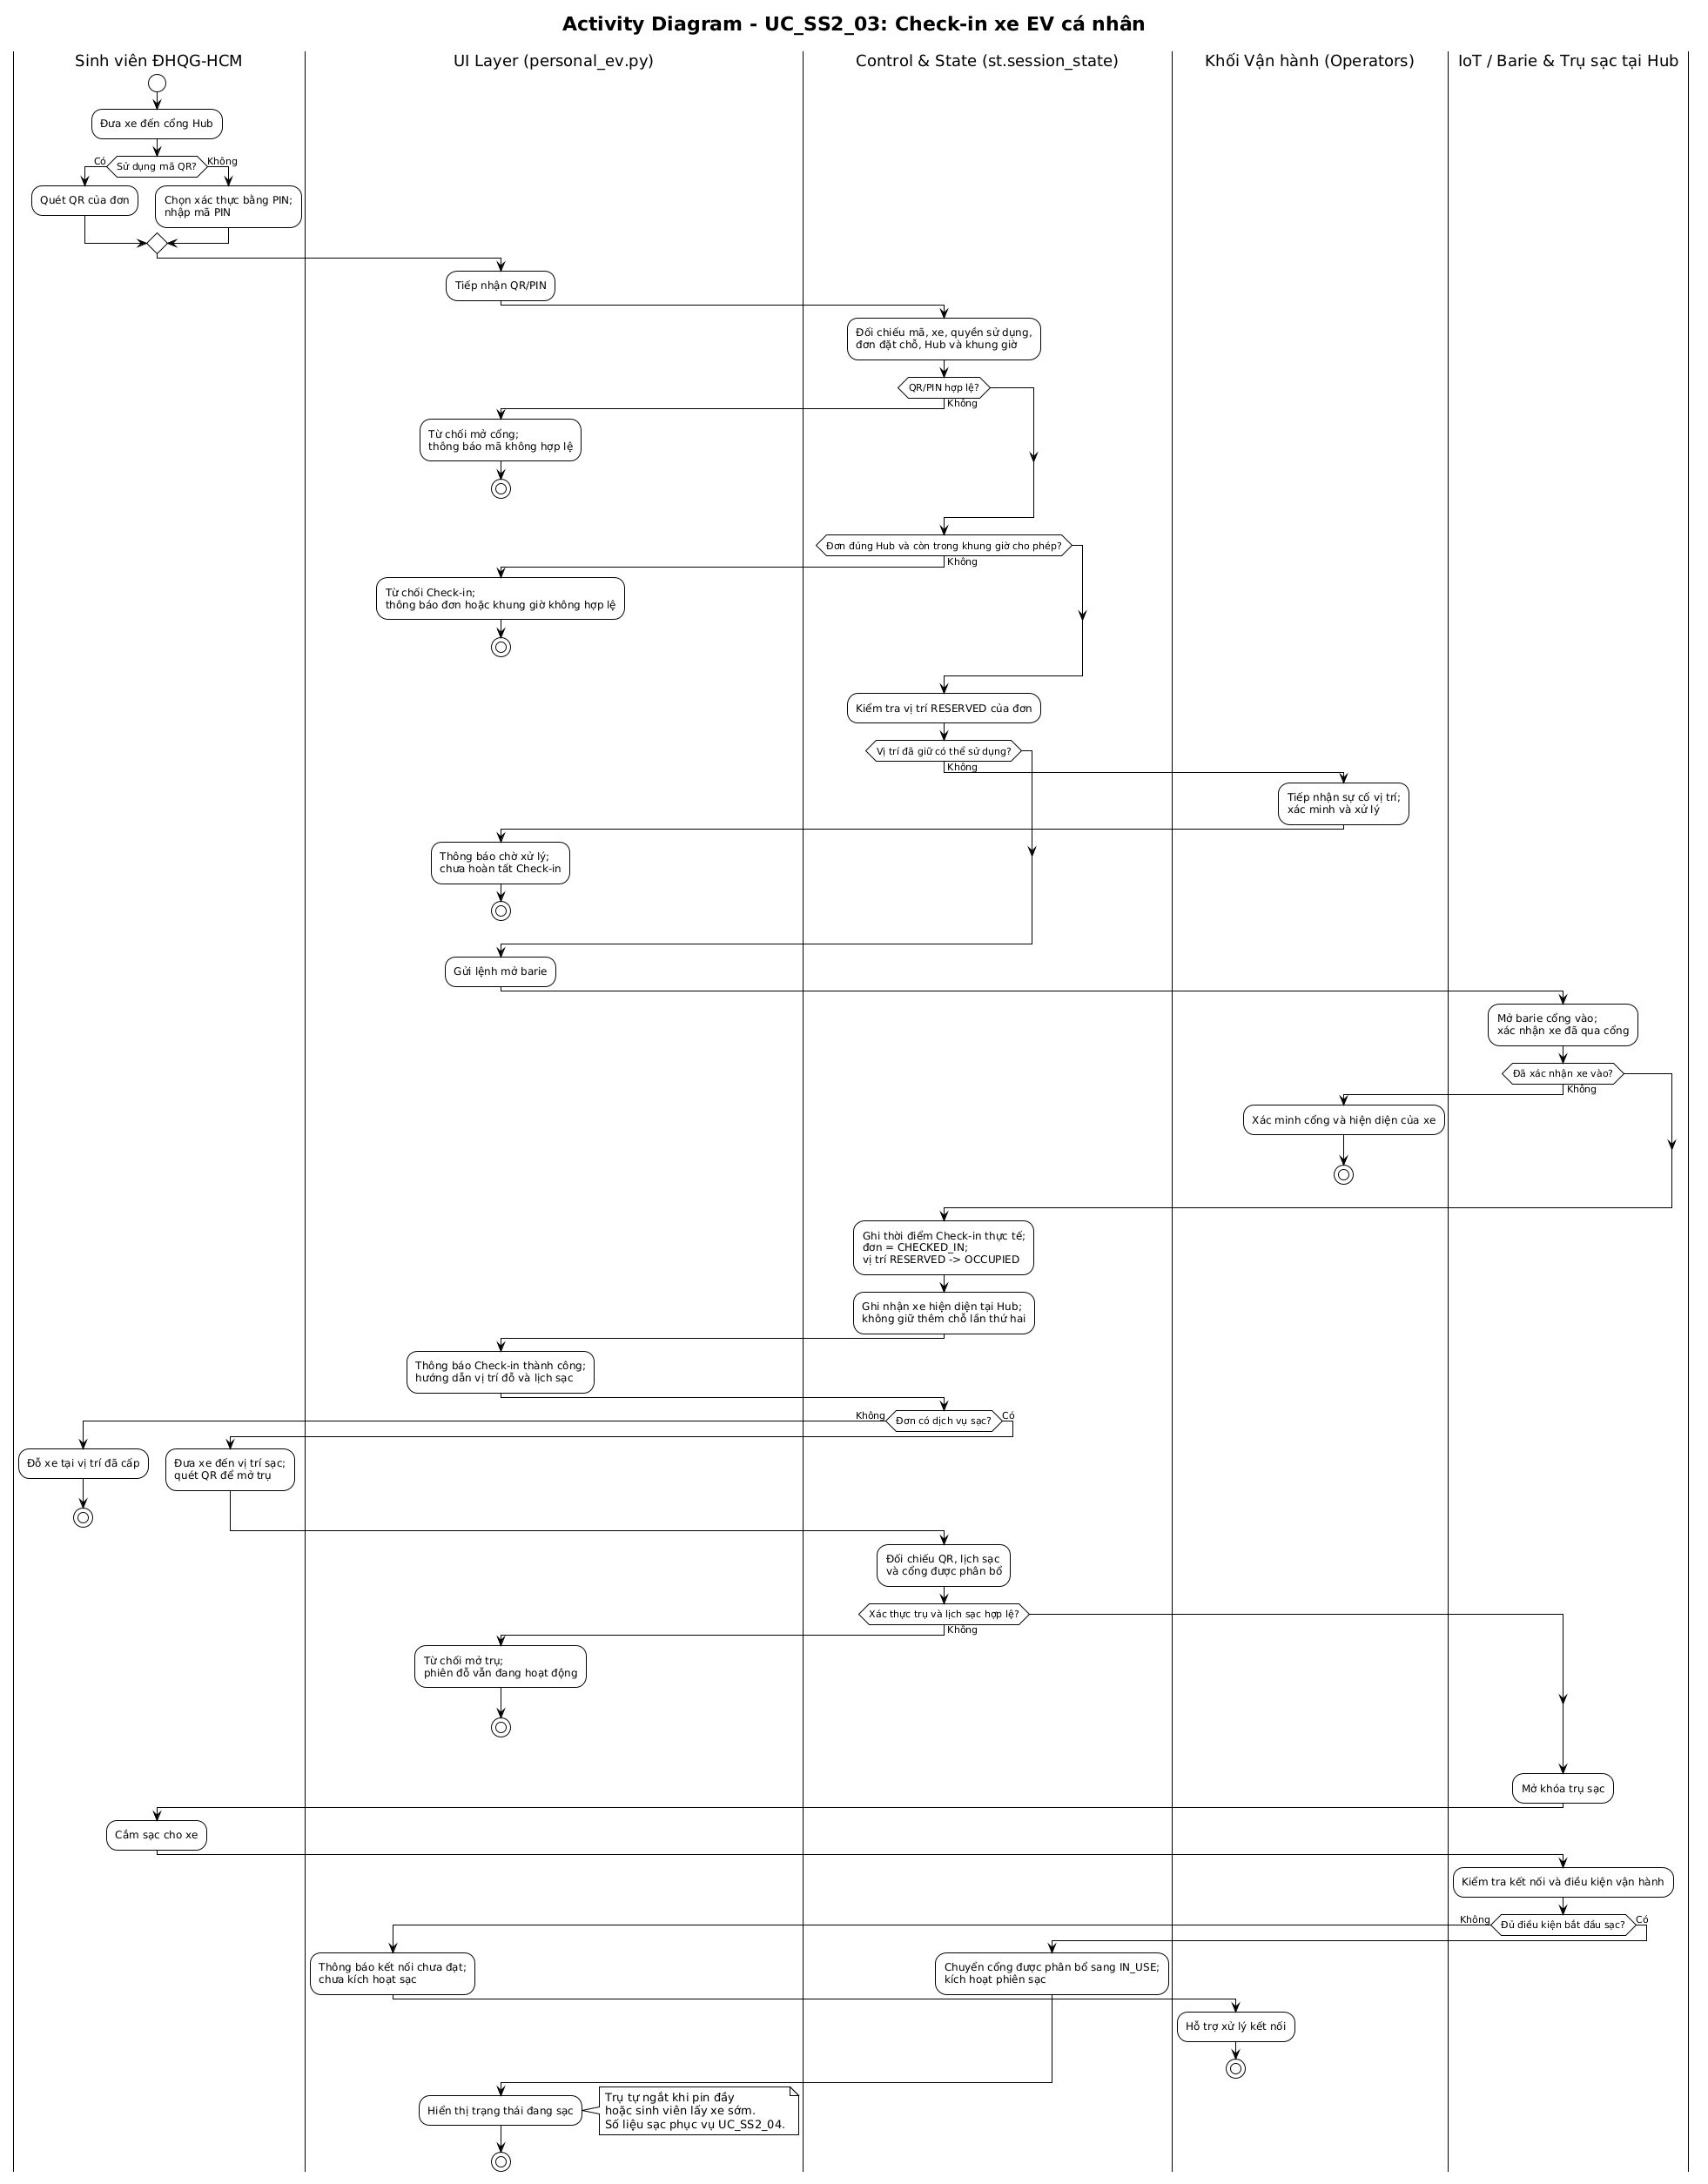
\includegraphics[width=0.92\textwidth,height=0.68\textheight,keepaspectratio]{Use-case detail-scenario/SS2/Activity diagrams/UC_SS2_03_NguyenAnhTai_activity.png}
    \caption{Sơ đồ Hoạt động Phân làn -- UC\_SS2\_03}
    \label{fig:act-ss2-03}
\end{figure}

\subsubsection{UC\_SS2\_04: Check-out và thanh toán dịch vụ xe cá nhân}
\begin{figure}[H]
    \centering
    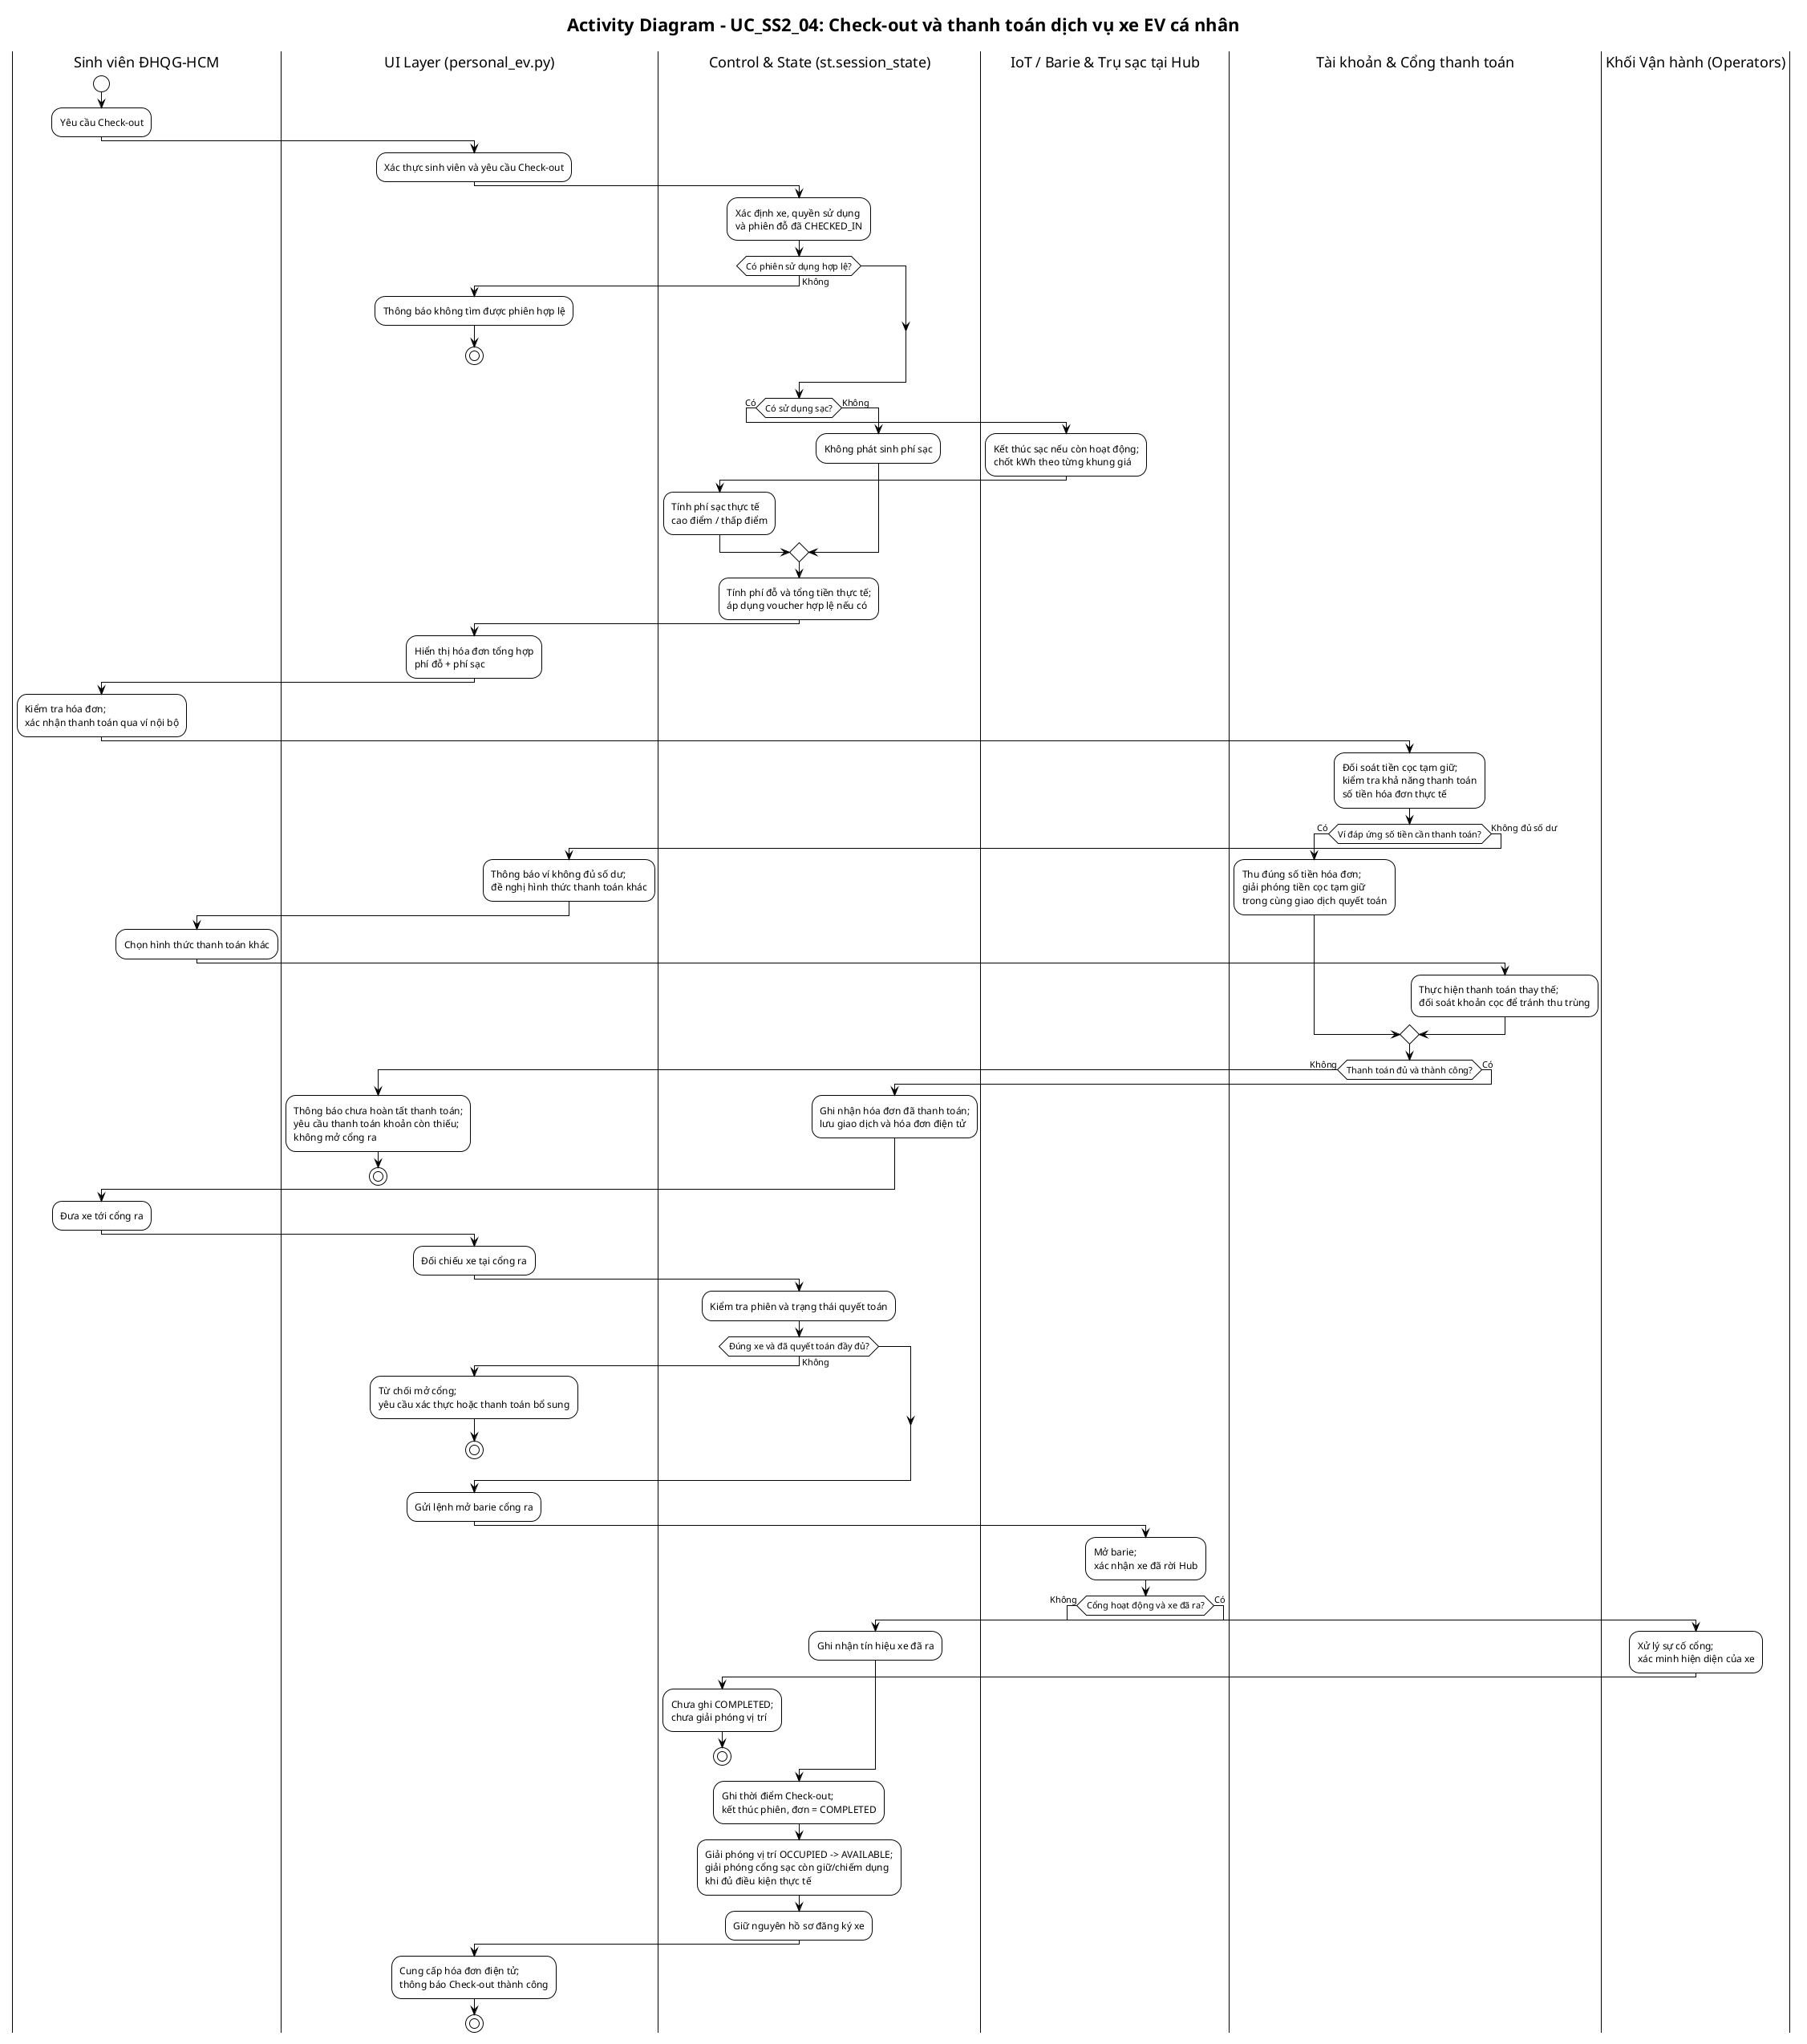
\includegraphics[width=0.92\textwidth,height=0.68\textheight,keepaspectratio]{Use-case detail-scenario/SS2/Activity diagrams/UC_SS2_04_NguyenAnhTai_activity.png}
    \caption{Sơ đồ Hoạt động Phân làn -- UC\_SS2\_04}
    \label{fig:act-ss2-04}
\end{figure}

\subsection{Phân hệ SS3: Giám sát Mạng lưới Hub (Phạm Tiến Đạt)}
\subsubsection{UC\_SS3\_01: Giám sát trạng thái Hub theo thời gian thực}
\begin{figure}[H]
    \centering
    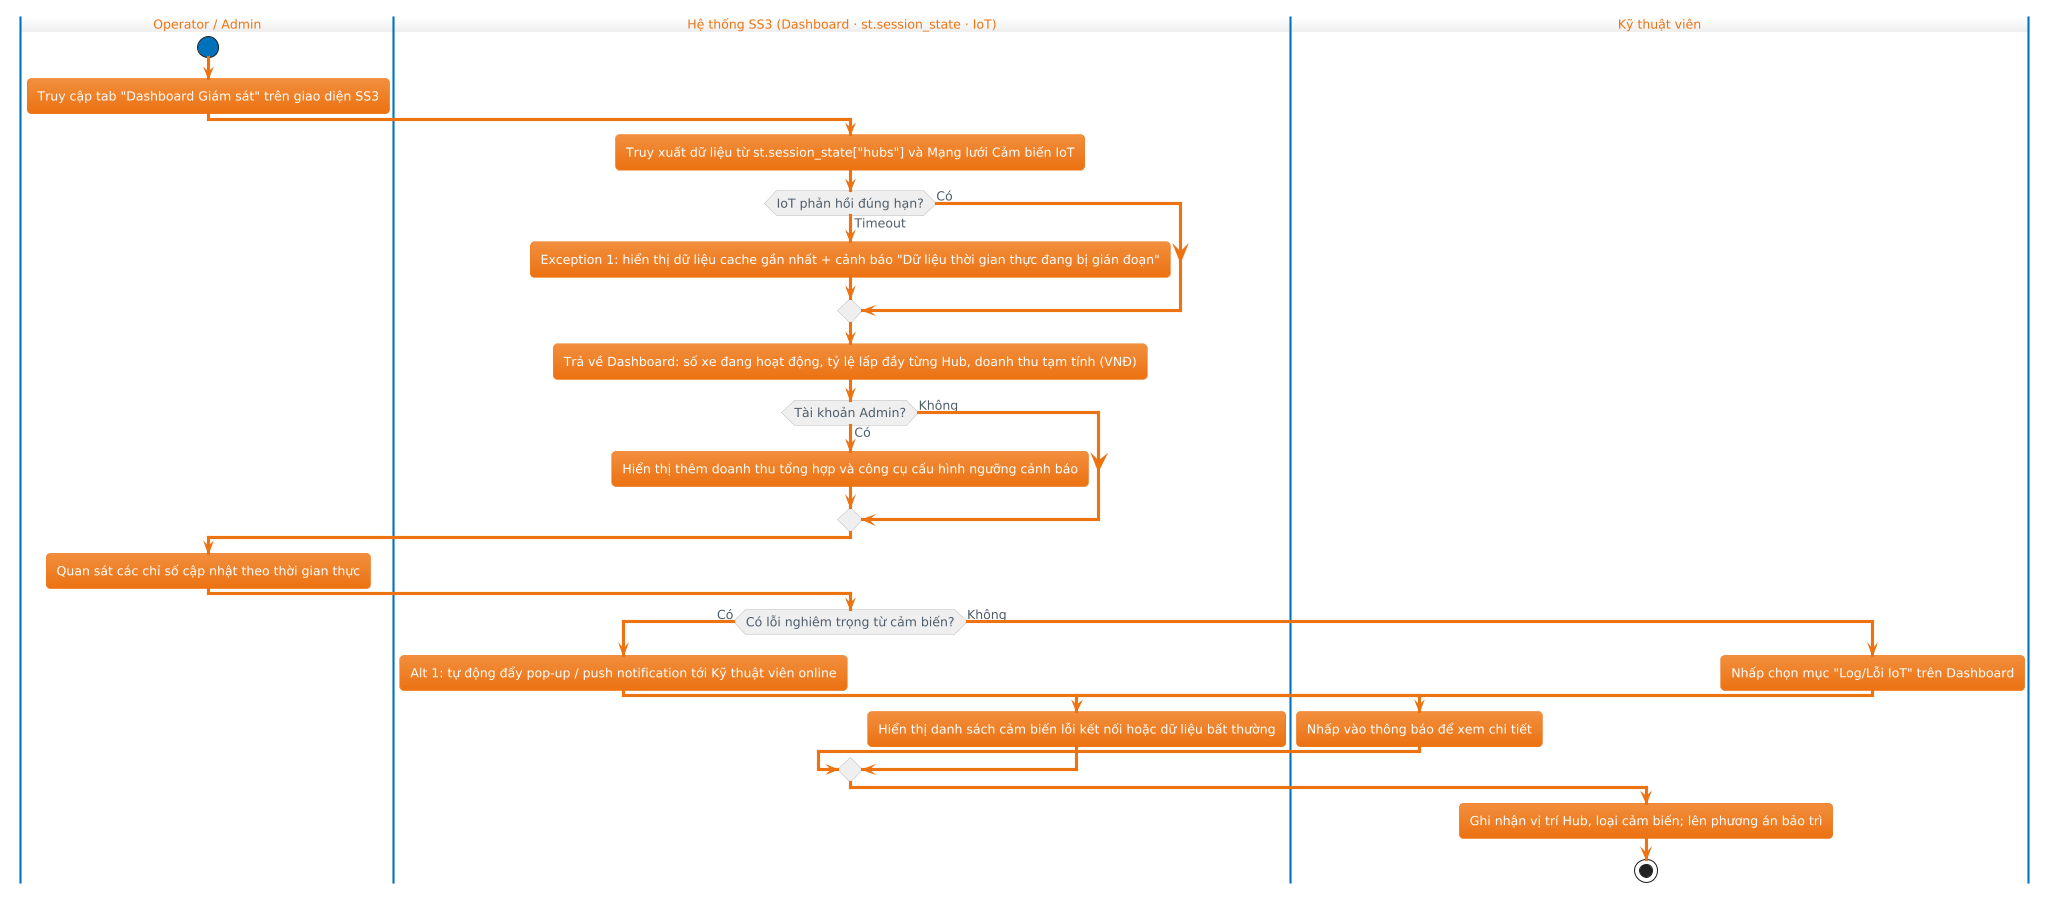
\includegraphics[width=0.92\textwidth,height=0.68\textheight,keepaspectratio]{Use-case detail-scenario/SS3/Activity diagrams/UC_SS3_01_PhamTienDat_activity.png}
    \caption{Sơ đồ Hoạt động Phân làn -- UC\_SS3\_01}
    \label{fig:act-ss3-01}
\end{figure}

\clearpage
\begin{landscape}
\subsubsection{UC\_SS3\_02: Cảnh báo quá tải \& Đề xuất điều phối}
\begin{figure}[H]
    \centering
    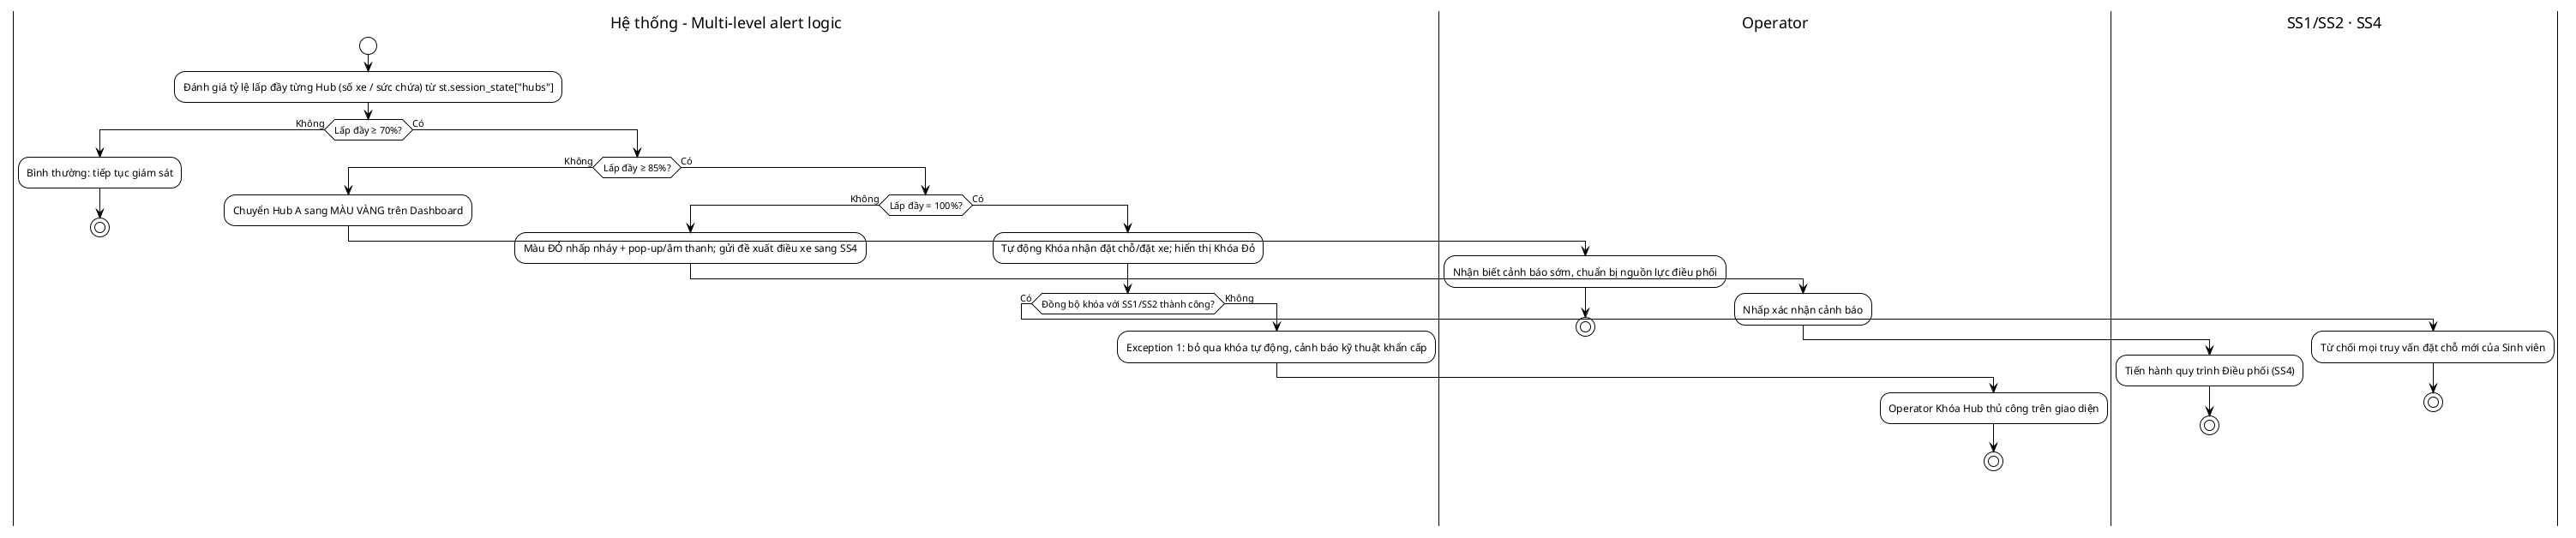
\includegraphics[width=0.98\linewidth,height=0.78\textheight,keepaspectratio]{Use-case detail-scenario/SS3/Activity diagrams/UC_SS3_02_PhamTienDat_activity.png}
    \caption{Sơ đồ Hoạt động Phân làn (Swimlane) -- UC\_SS3\_02 (Cảnh báo quá tải \& Đề xuất điều phối)}
    \label{fig:act-ss3-02}
\end{figure}
\end{landscape}
\clearpage

\subsection{Phân hệ SS4: Điều phối \& Xử lý Sự cố (Đặng Hoàng Quý Nhân)}
\subsubsection{UC\_SS4\_01: Lập lệnh điều phối phương tiện giữa các Hub}
\begin{figure}[H]
    \centering
    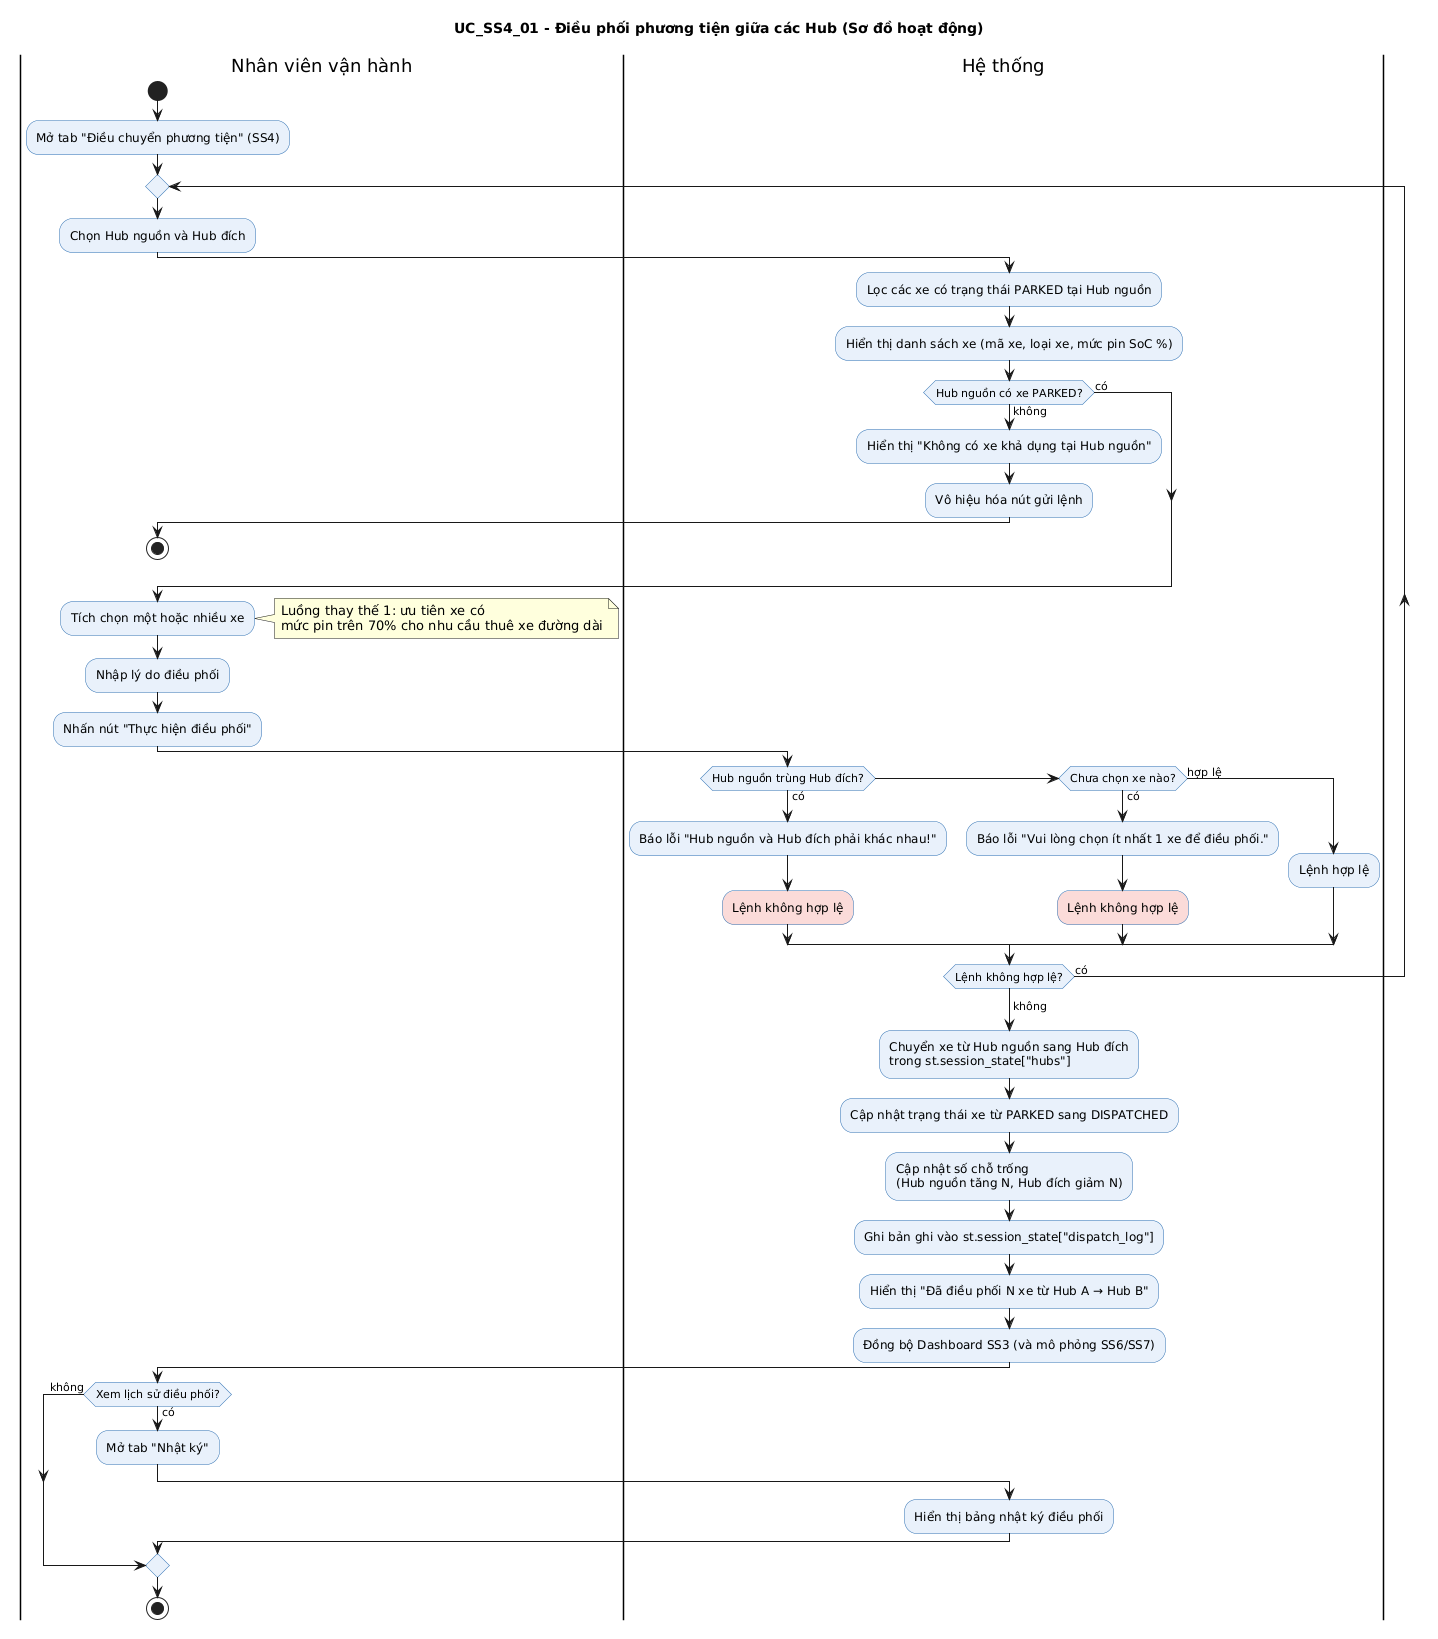
\includegraphics[width=0.92\textwidth,height=0.68\textheight,keepaspectratio]{Use-case detail-scenario/SS4/Activity diagrams/UC_SS4_01_activity.png}
    \caption{Sơ đồ Hoạt động Phân làn -- UC\_SS4\_01}
    \label{fig:act-ss4-01}
\end{figure}

\subsubsection{UC\_SS4\_02: Báo cáo \& Xử lý sự cố kỹ thuật phương tiện}
\begin{figure}[H]
    \centering
    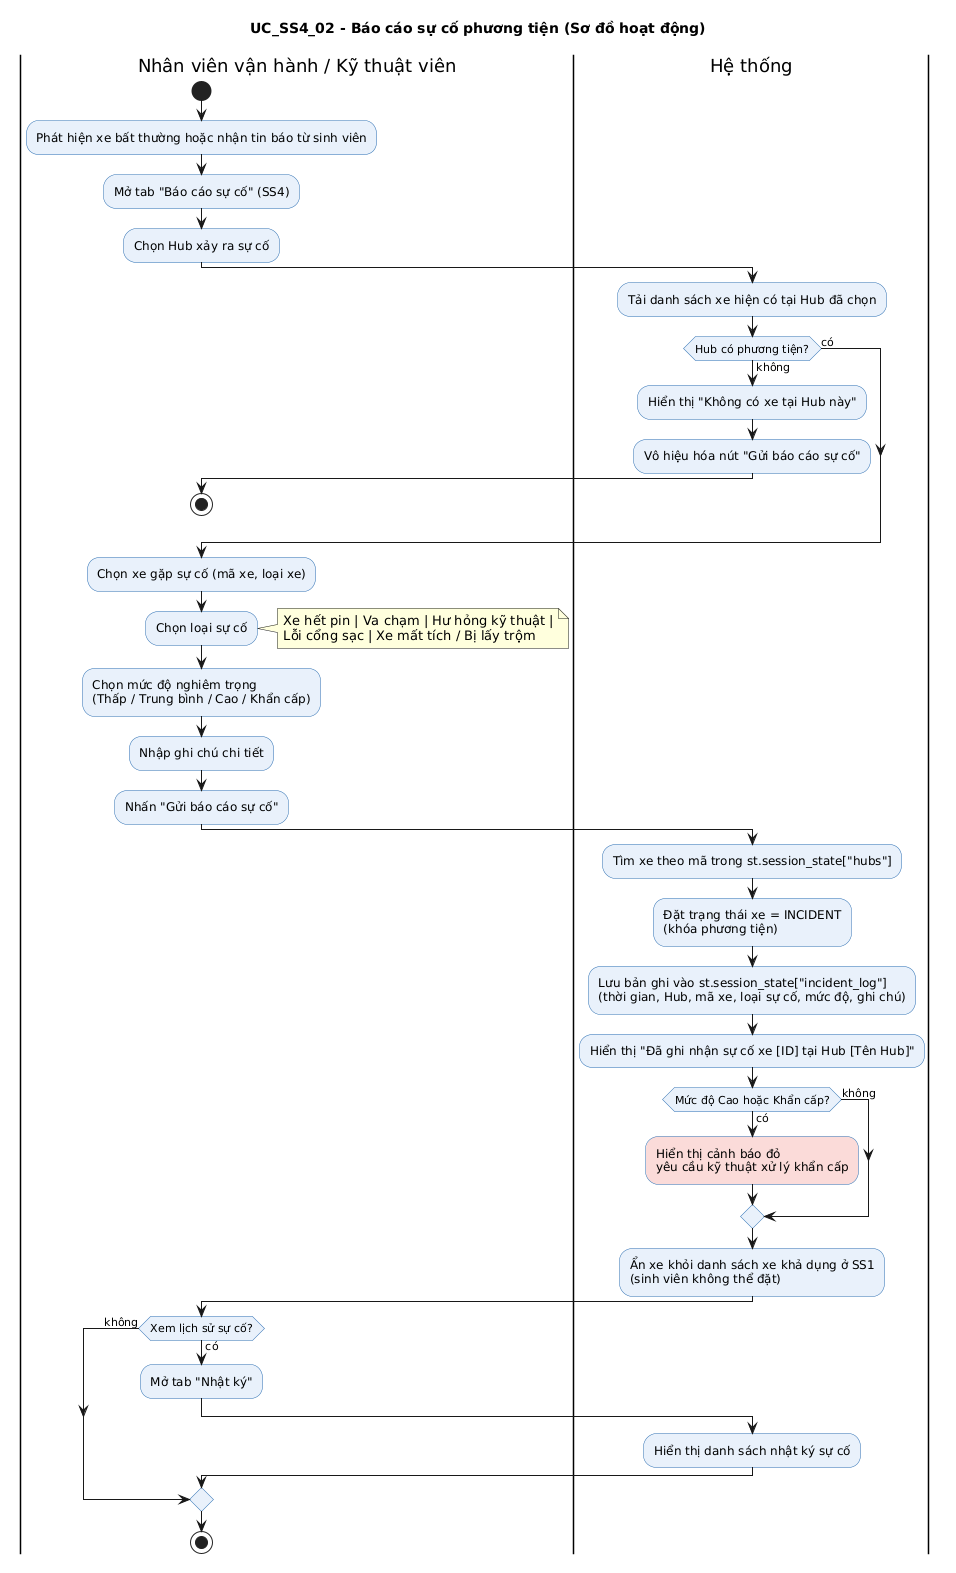
\includegraphics[width=0.92\textwidth,height=0.68\textheight,keepaspectratio]{Use-case detail-scenario/SS4/Activity diagrams/UC_SS4_02_activity.png}
    \caption{Sơ đồ Hoạt động Phân làn -- UC\_SS4\_02}
    \label{fig:act-ss4-02}
\end{figure}

\subsection{Phân hệ SS5: Lập lịch Sạc Thông minh (Dương Đăng Khoa)}
\subsubsection{UC\_SS5\_01: Lập lịch ưu tiên sạc tự động}
\begin{figure}[H]
    \centering
    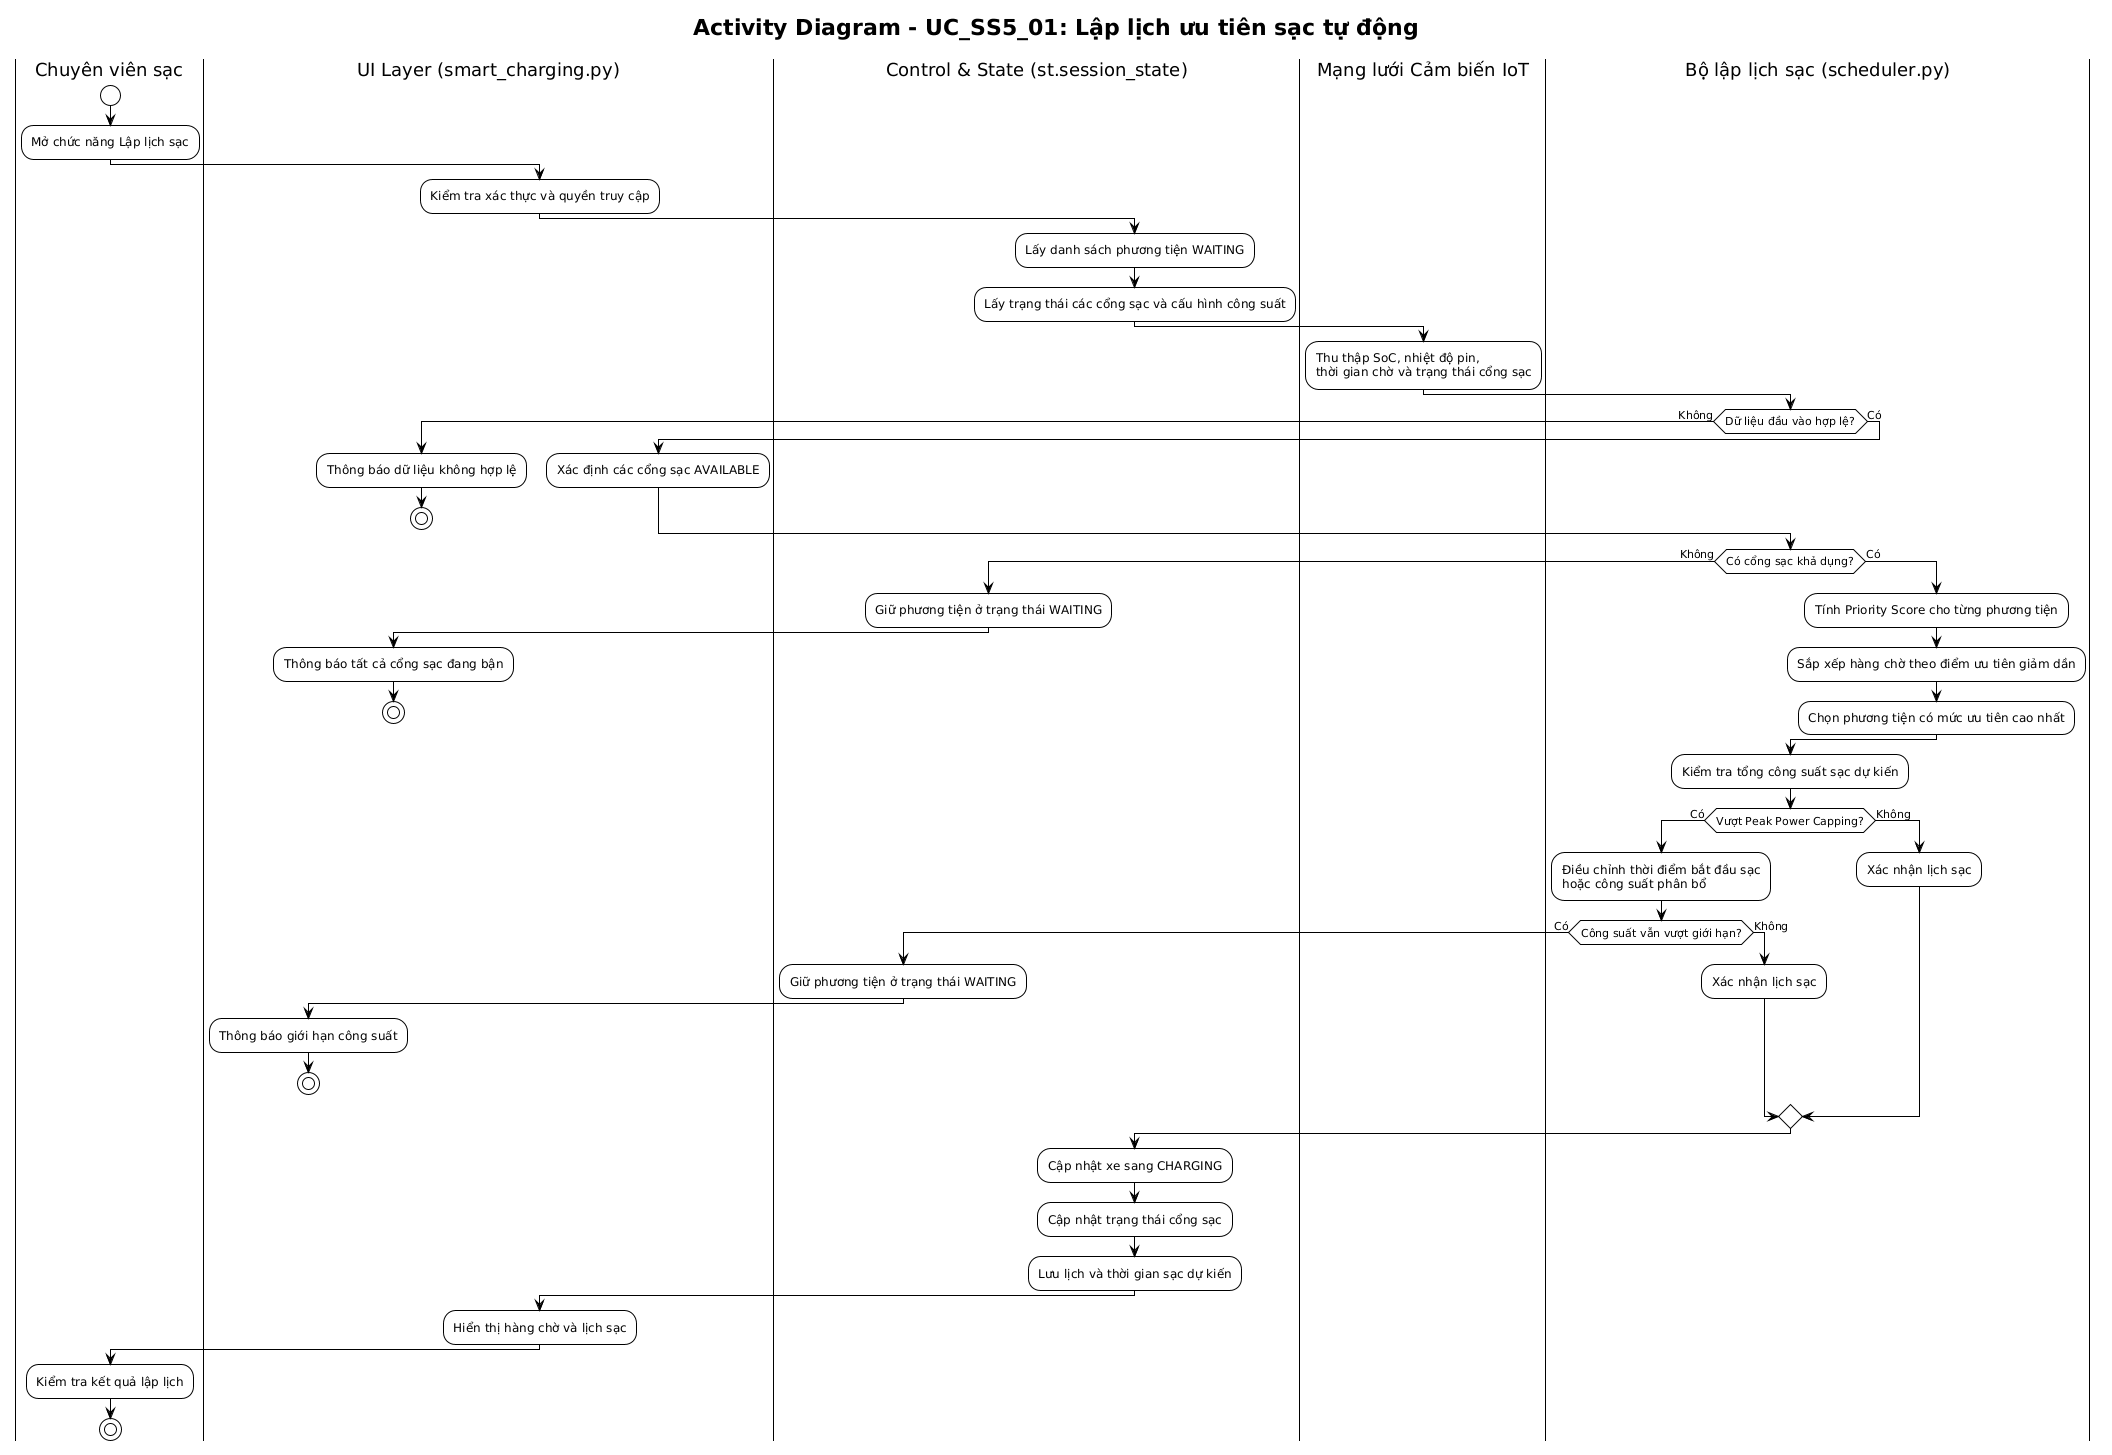
\includegraphics[width=0.92\textwidth,height=0.68\textheight,keepaspectratio]{Use-case detail-scenario/SS5/Activity diagrams/UC_SS5_01_DuongDangKhoa_activity.png}
    \caption{Sơ đồ Hoạt động Phân làn -- UC\_SS5\_01}
    \label{fig:act-ss5-01}
\end{figure}

\subsubsection{UC\_SS5\_02: Giám sát hàng đợi sạc \& Phí chiếm dụng}
\begin{figure}[H]
    \centering
    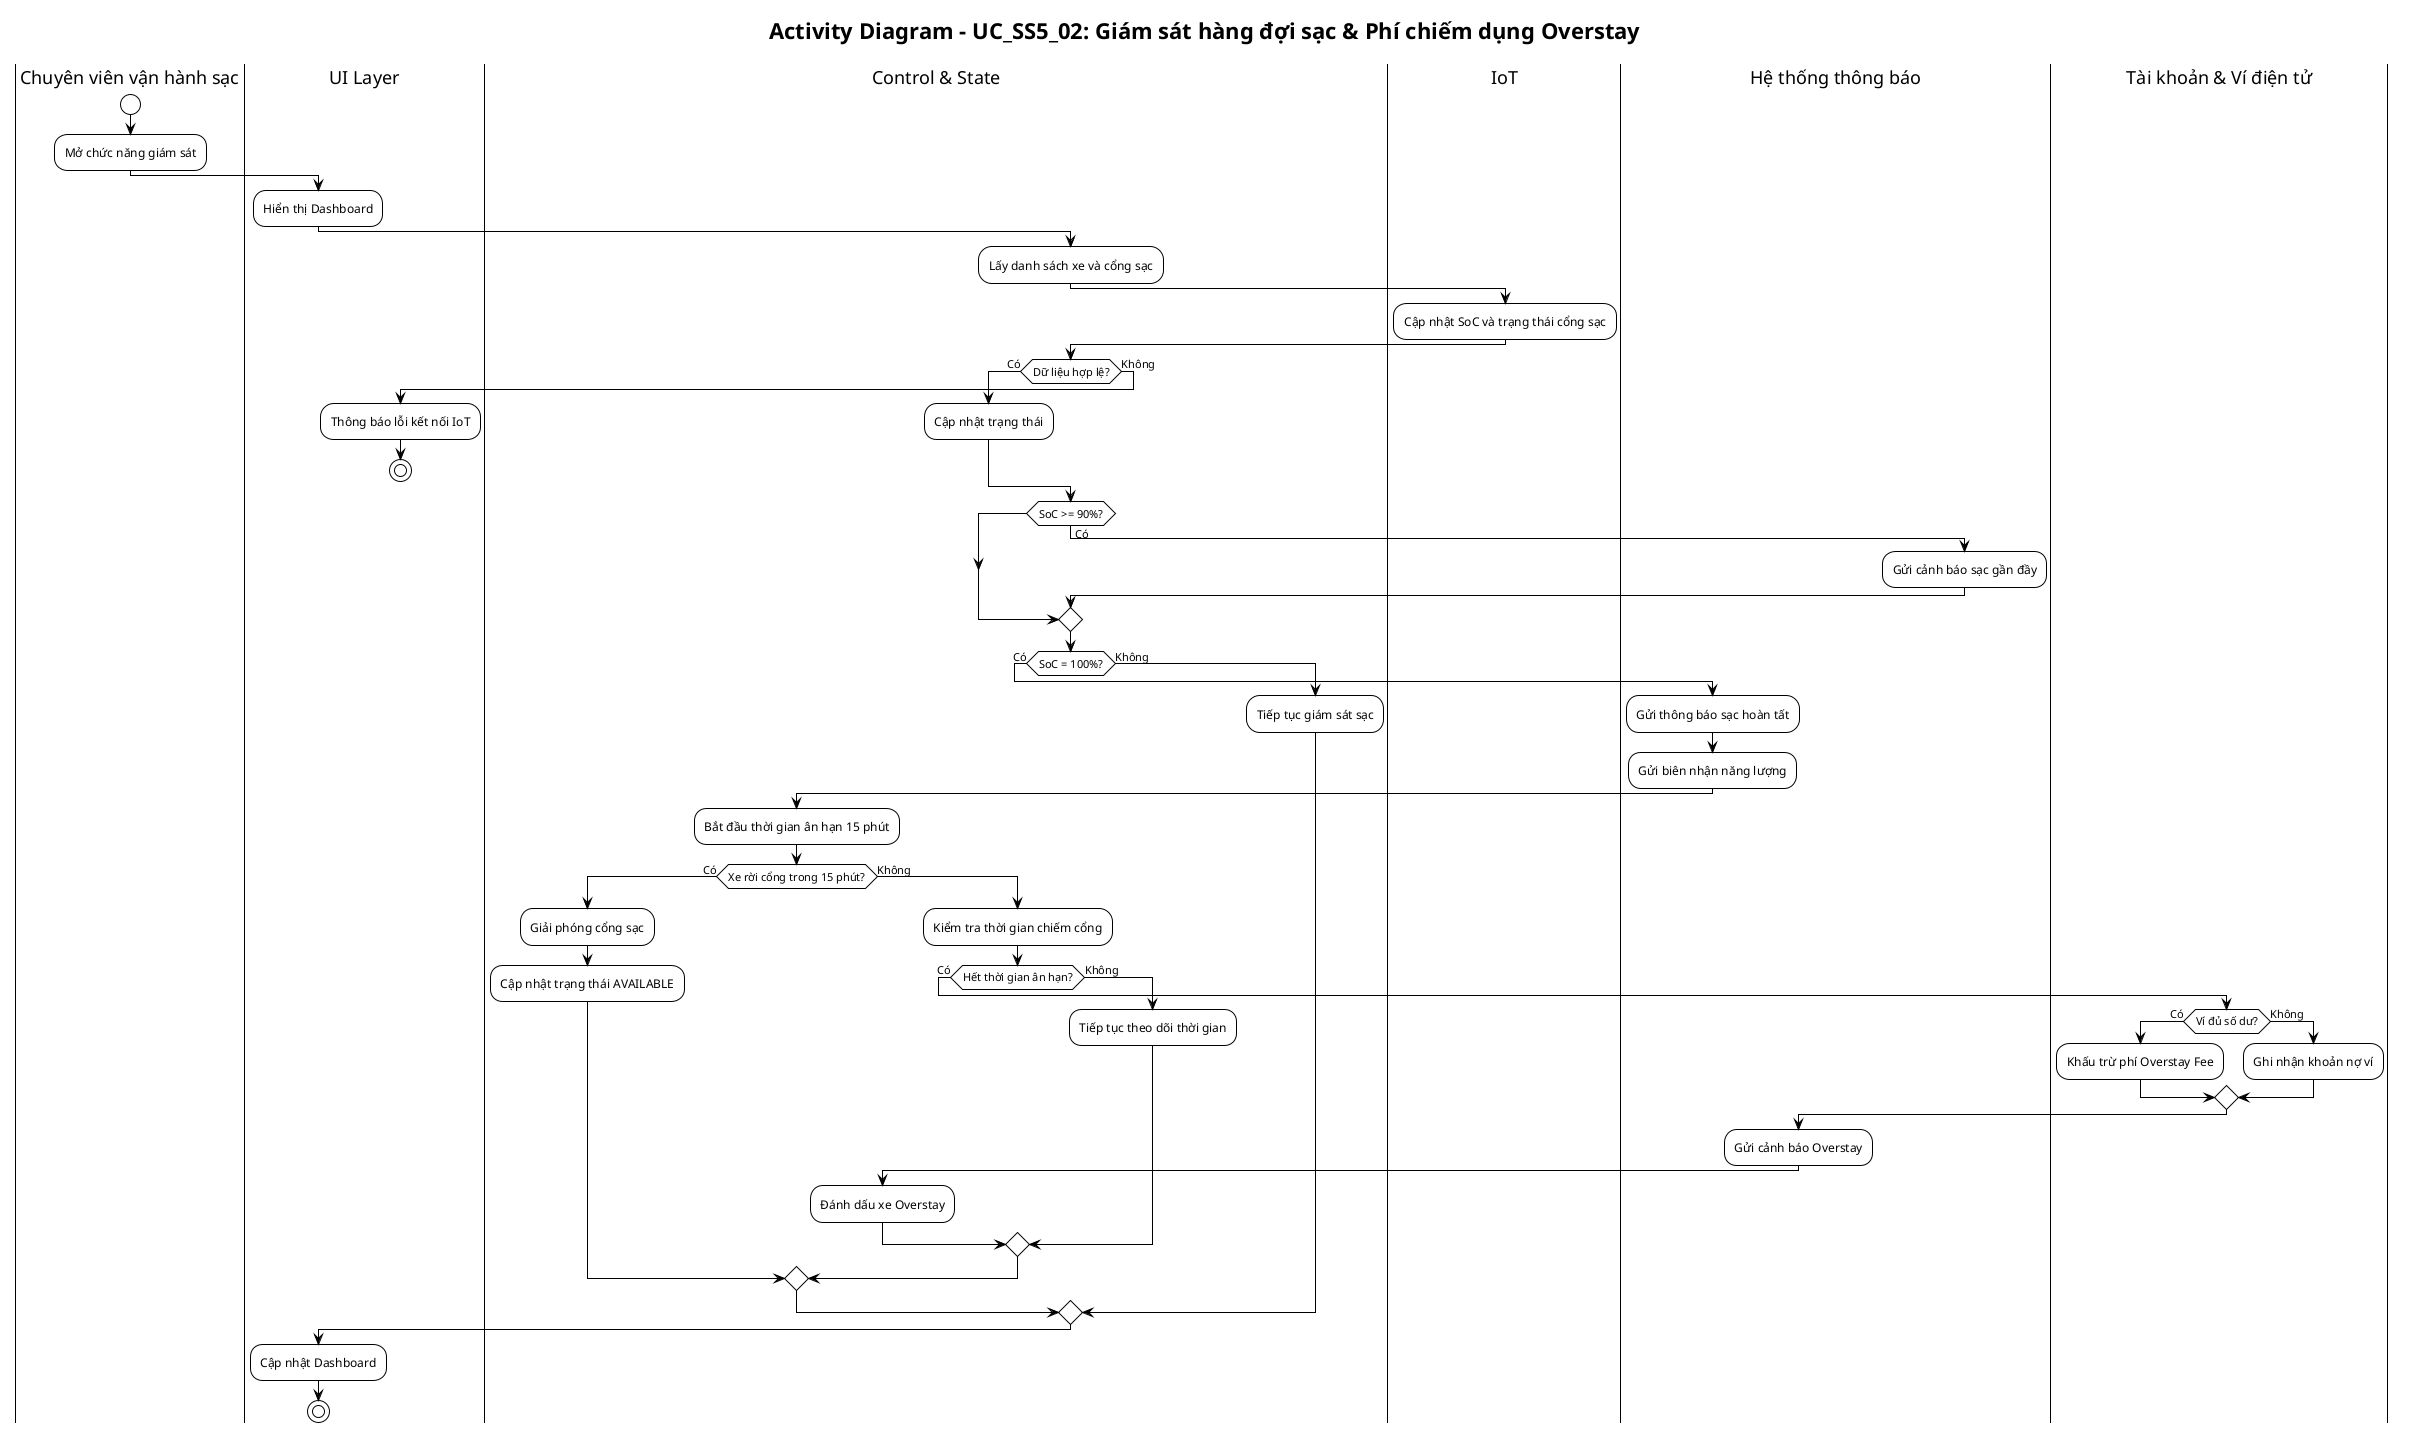
\includegraphics[width=0.92\textwidth,height=0.68\textheight,keepaspectratio]{Use-case detail-scenario/SS5/Activity diagrams/UC_SS5_02_DuongDangKhoa_activity.png}
    \caption{Sơ đồ Hoạt động Phân làn -- UC\_SS5\_02}
    \label{fig:act-ss5-02}
\end{figure}

\subsection{Phân hệ SS6: Mô phỏng What-if Nhu cầu (Hoàng Văn Tấn)}
\subsubsection{UC\_SS6\_01: Mô phỏng đợt tăng đột biến hành khách Metro (Metro Surge)}
\begin{figure}[H]
    \centering
    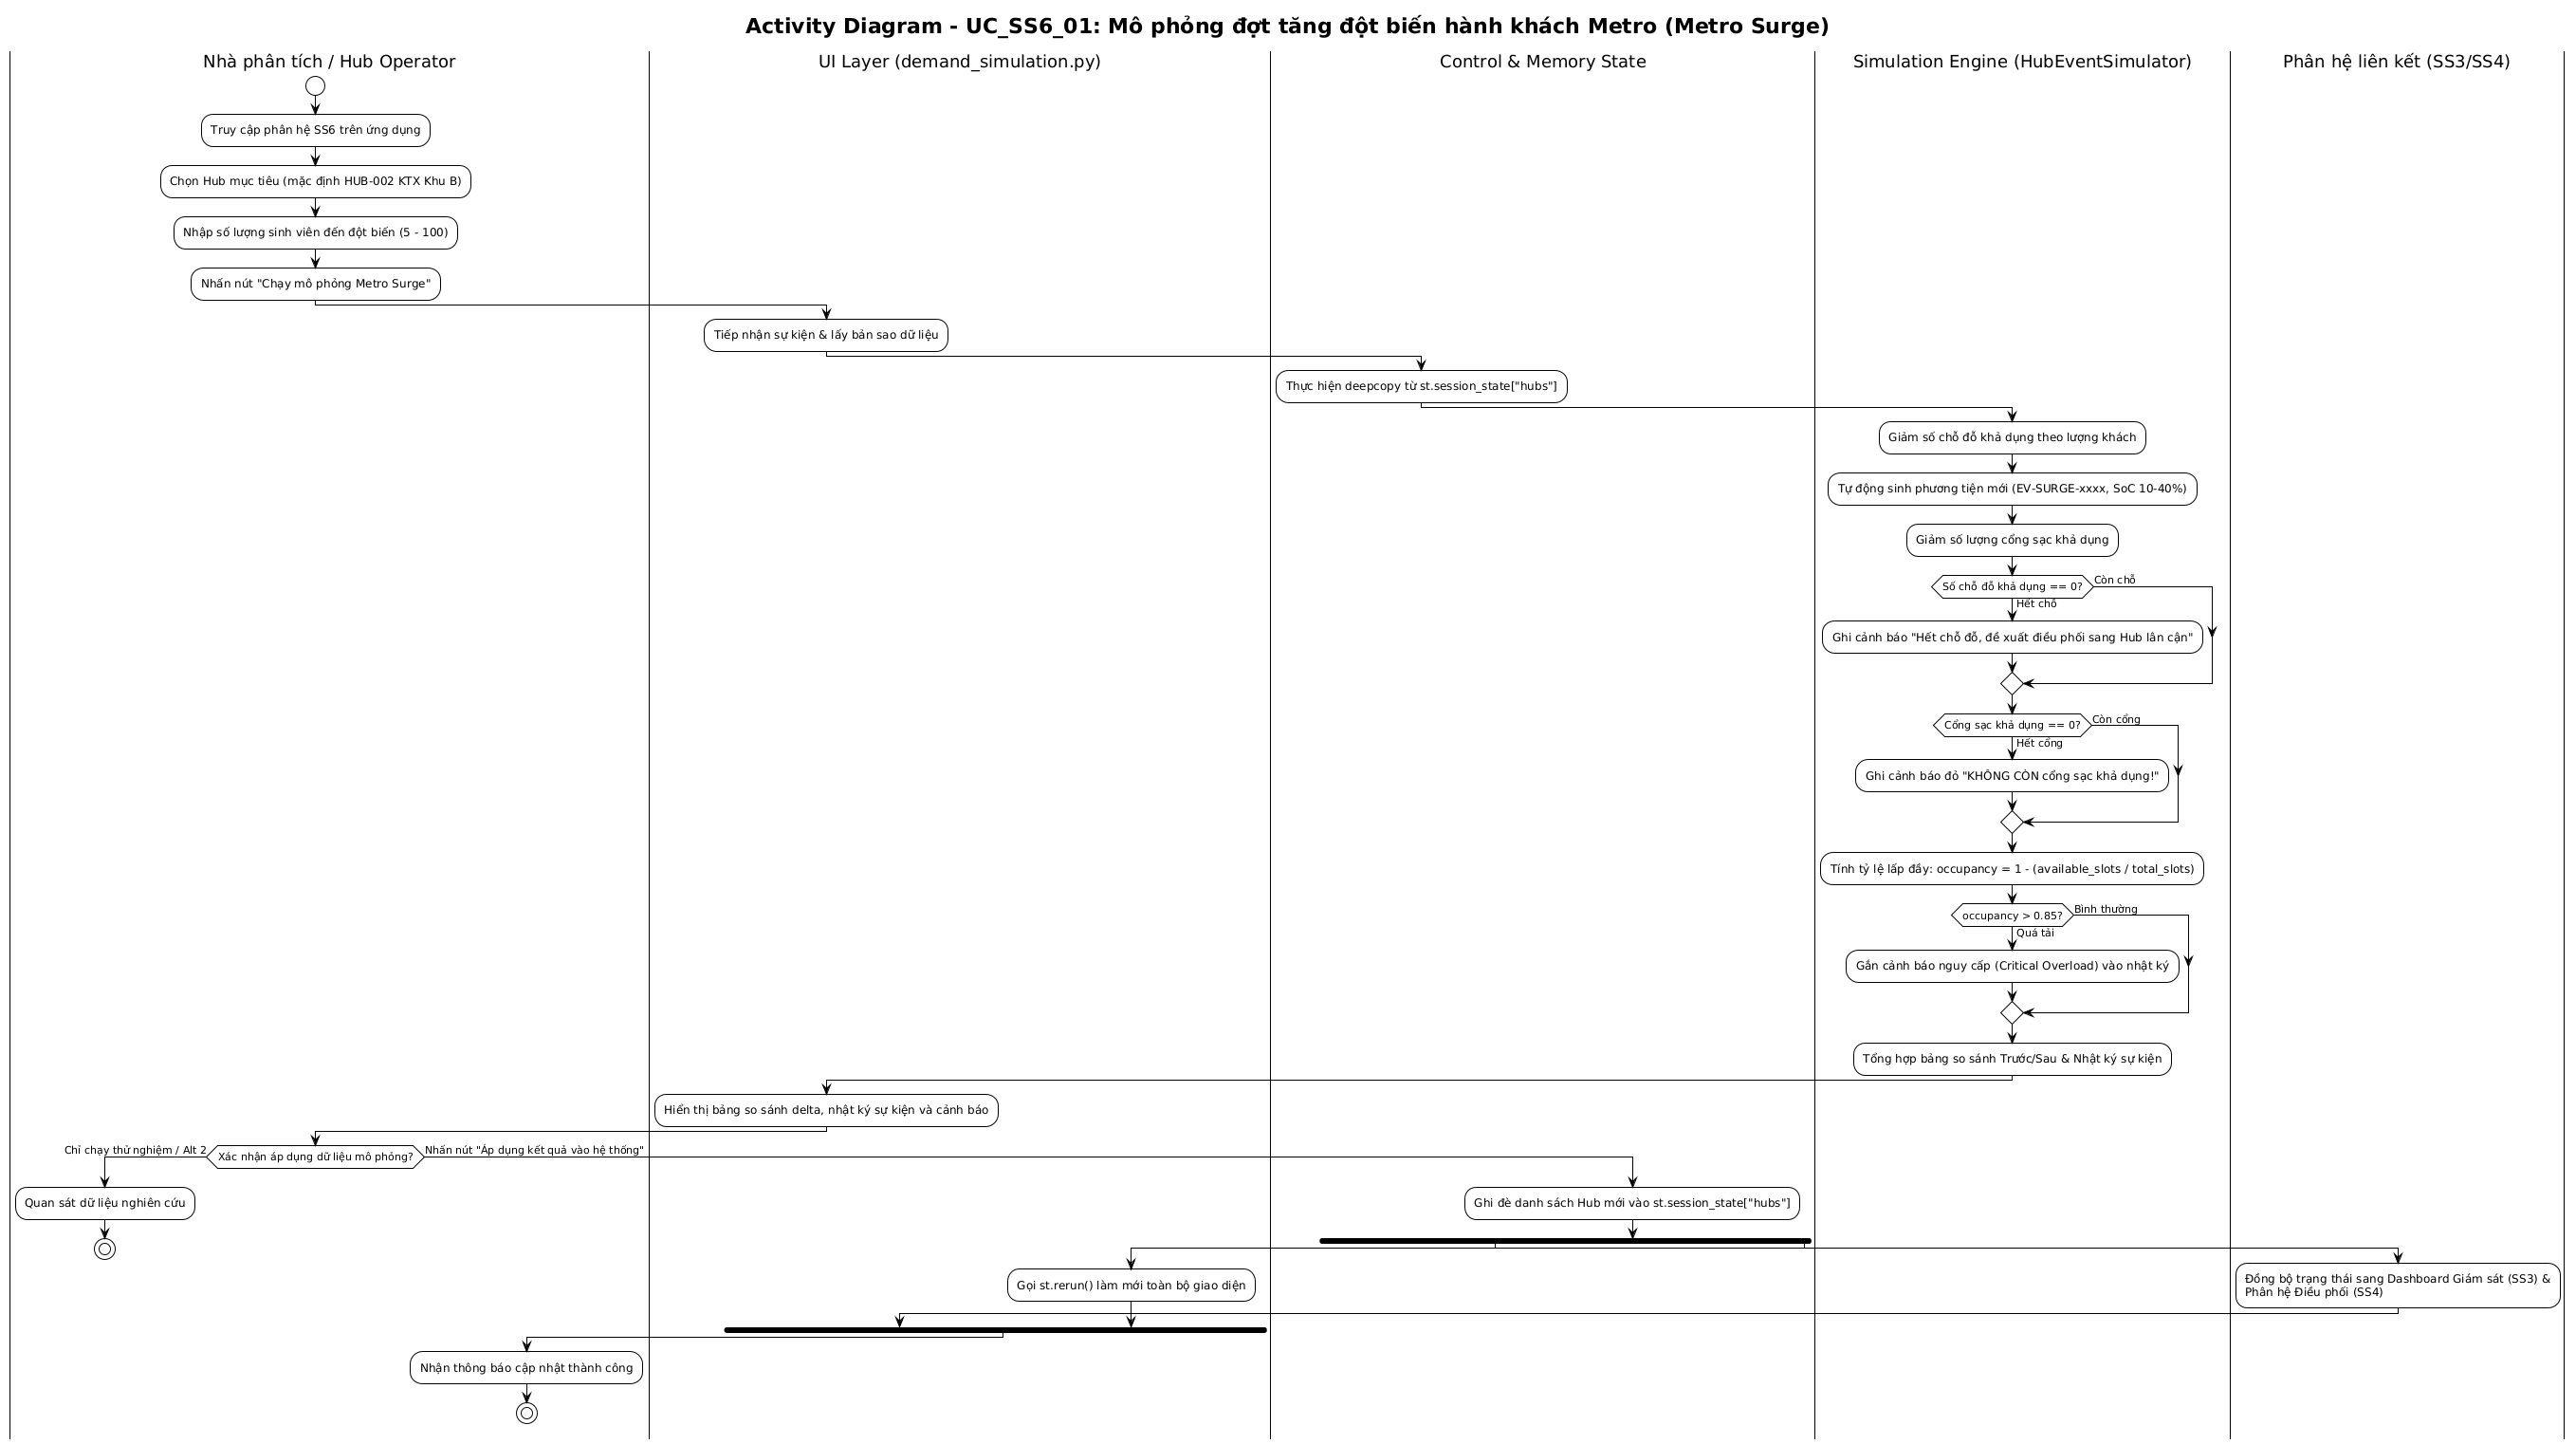
\includegraphics[width=0.98\textwidth,height=0.75\textheight,keepaspectratio]{Use-case detail-scenario/SS6/Activity diagrams/UC_SS6_01_HoangVanTan_activity.png}
    \caption{Sơ đồ Hoạt động Phân làn -- UC\_SS6\_01}
    \label{fig:act-ss6-01}
\end{figure}

\subsubsection{UC\_SS6\_02: Dự báo nhu cầu theo giờ \& Phân tích hàng đợi}
\begin{figure}[H]
    \centering
    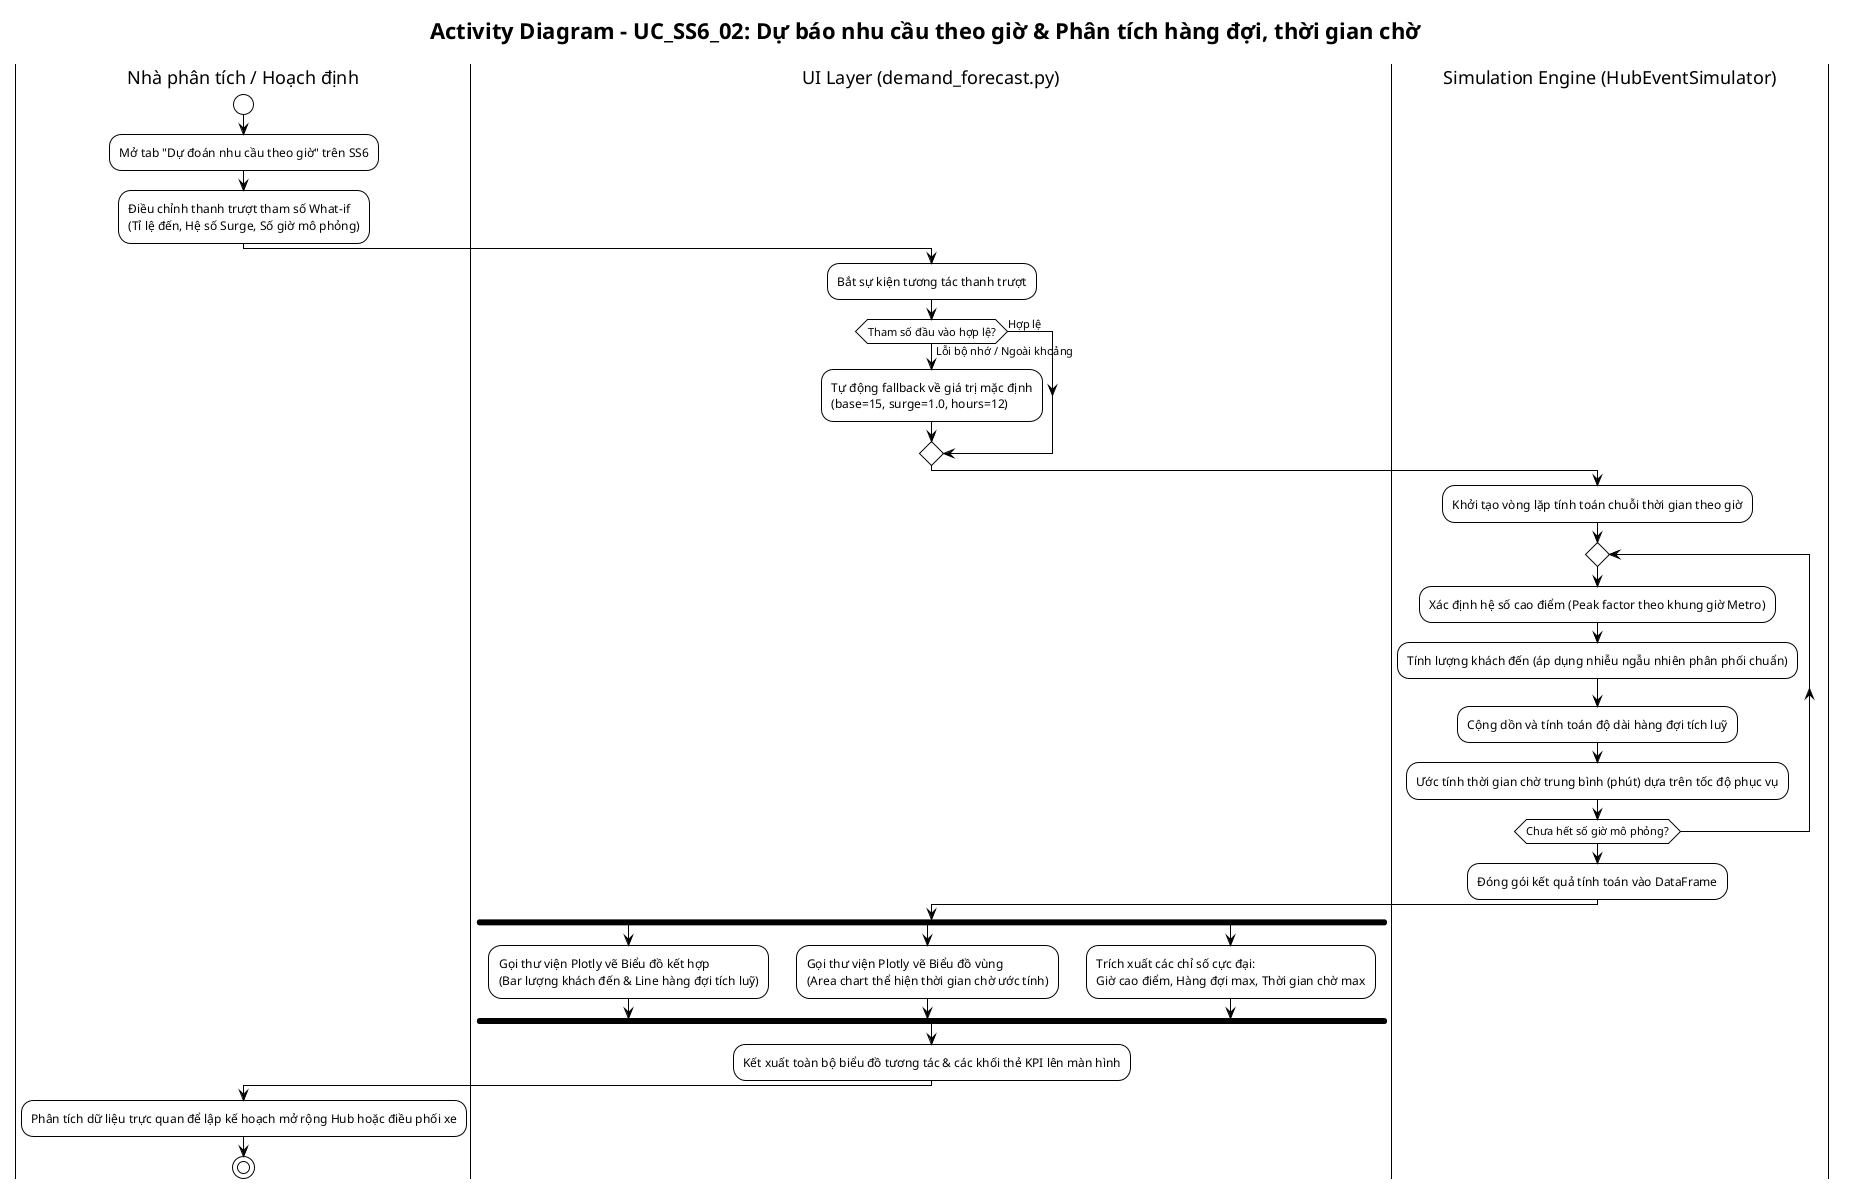
\includegraphics[width=0.98\textwidth,height=0.75\textheight,keepaspectratio]{Use-case detail-scenario/SS6/Activity diagrams/UC_SS6_02_HoangVanTan_activity.png}
    \caption{Sơ đồ Hoạt động Phân làn -- UC\_SS6\_02}
    \label{fig:act-ss6-02}
\end{figure}

\subsection{Phân hệ SS7: Mô phỏng What-if Hạ tầng (Nguyễn Trung Nguyên)}
\subsubsection{UC\_SS7\_01: Mô phỏng sự cố mất điện / lỗi cổng sạc}
\begin{figure}[H]
    \centering
    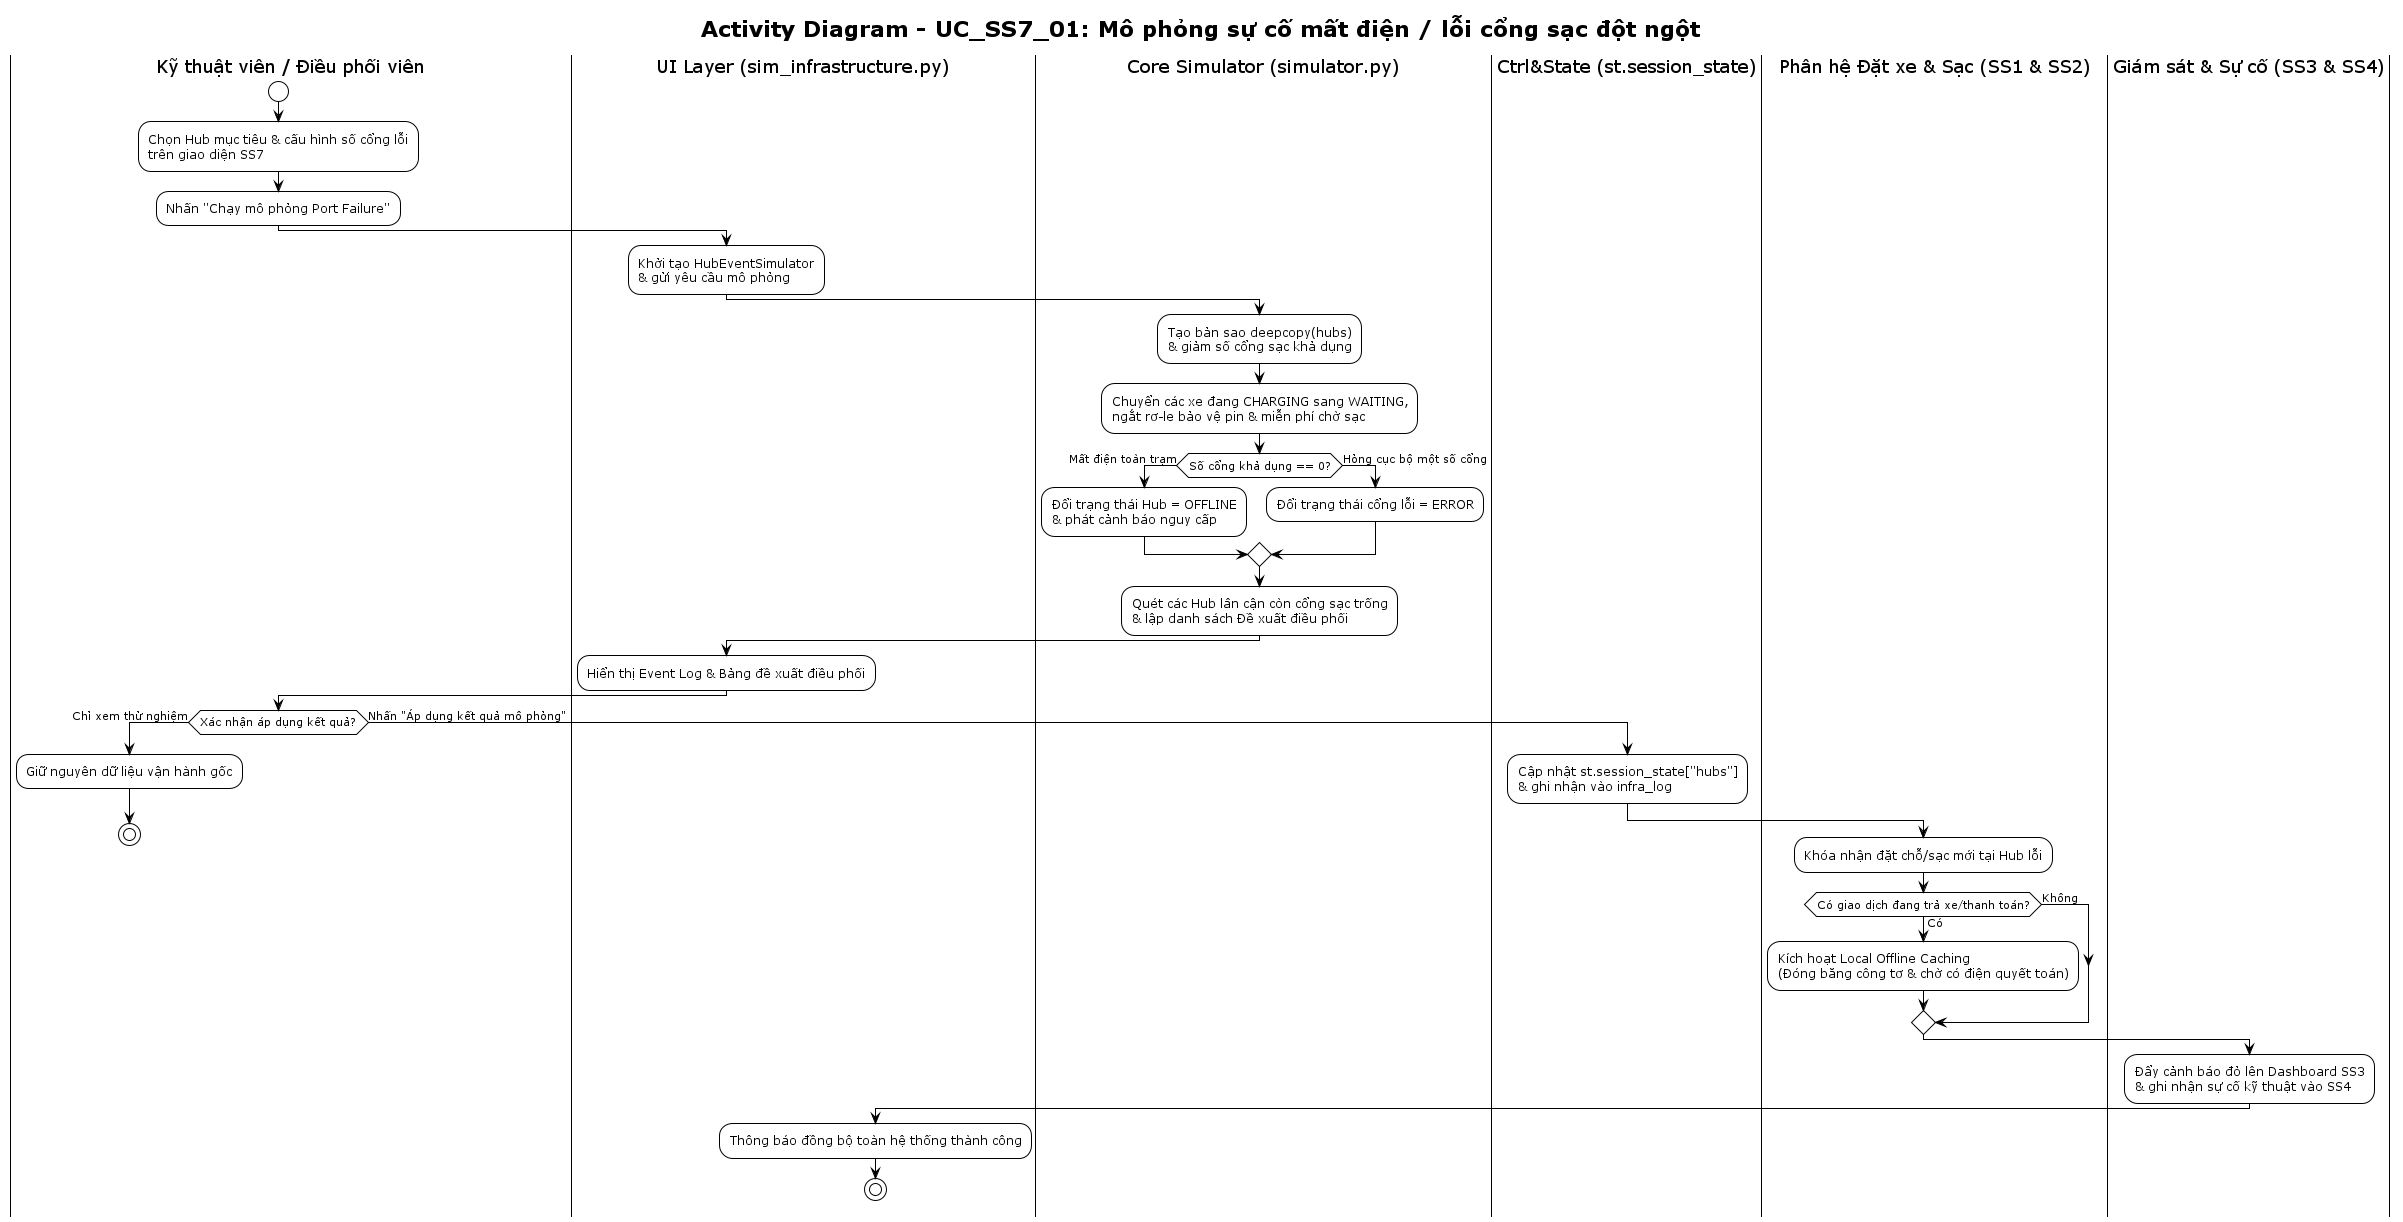
\includegraphics[width=0.98\textwidth,height=0.75\textheight,keepaspectratio]{Use-case detail-scenario/SS7/Activity diagrams/UC_SS7_01_NguyenTrungNguyen_activity.png}
    \caption{Sơ đồ Hoạt động Phân làn -- UC\_SS7\_01}
    \label{fig:act-ss7-01}
\end{figure}

\subsubsection{UC\_SS7\_02: Tự động phát cảnh báo \& Gợi ý điều hướng 1-chạm}
\begin{figure}[H]
    \centering
    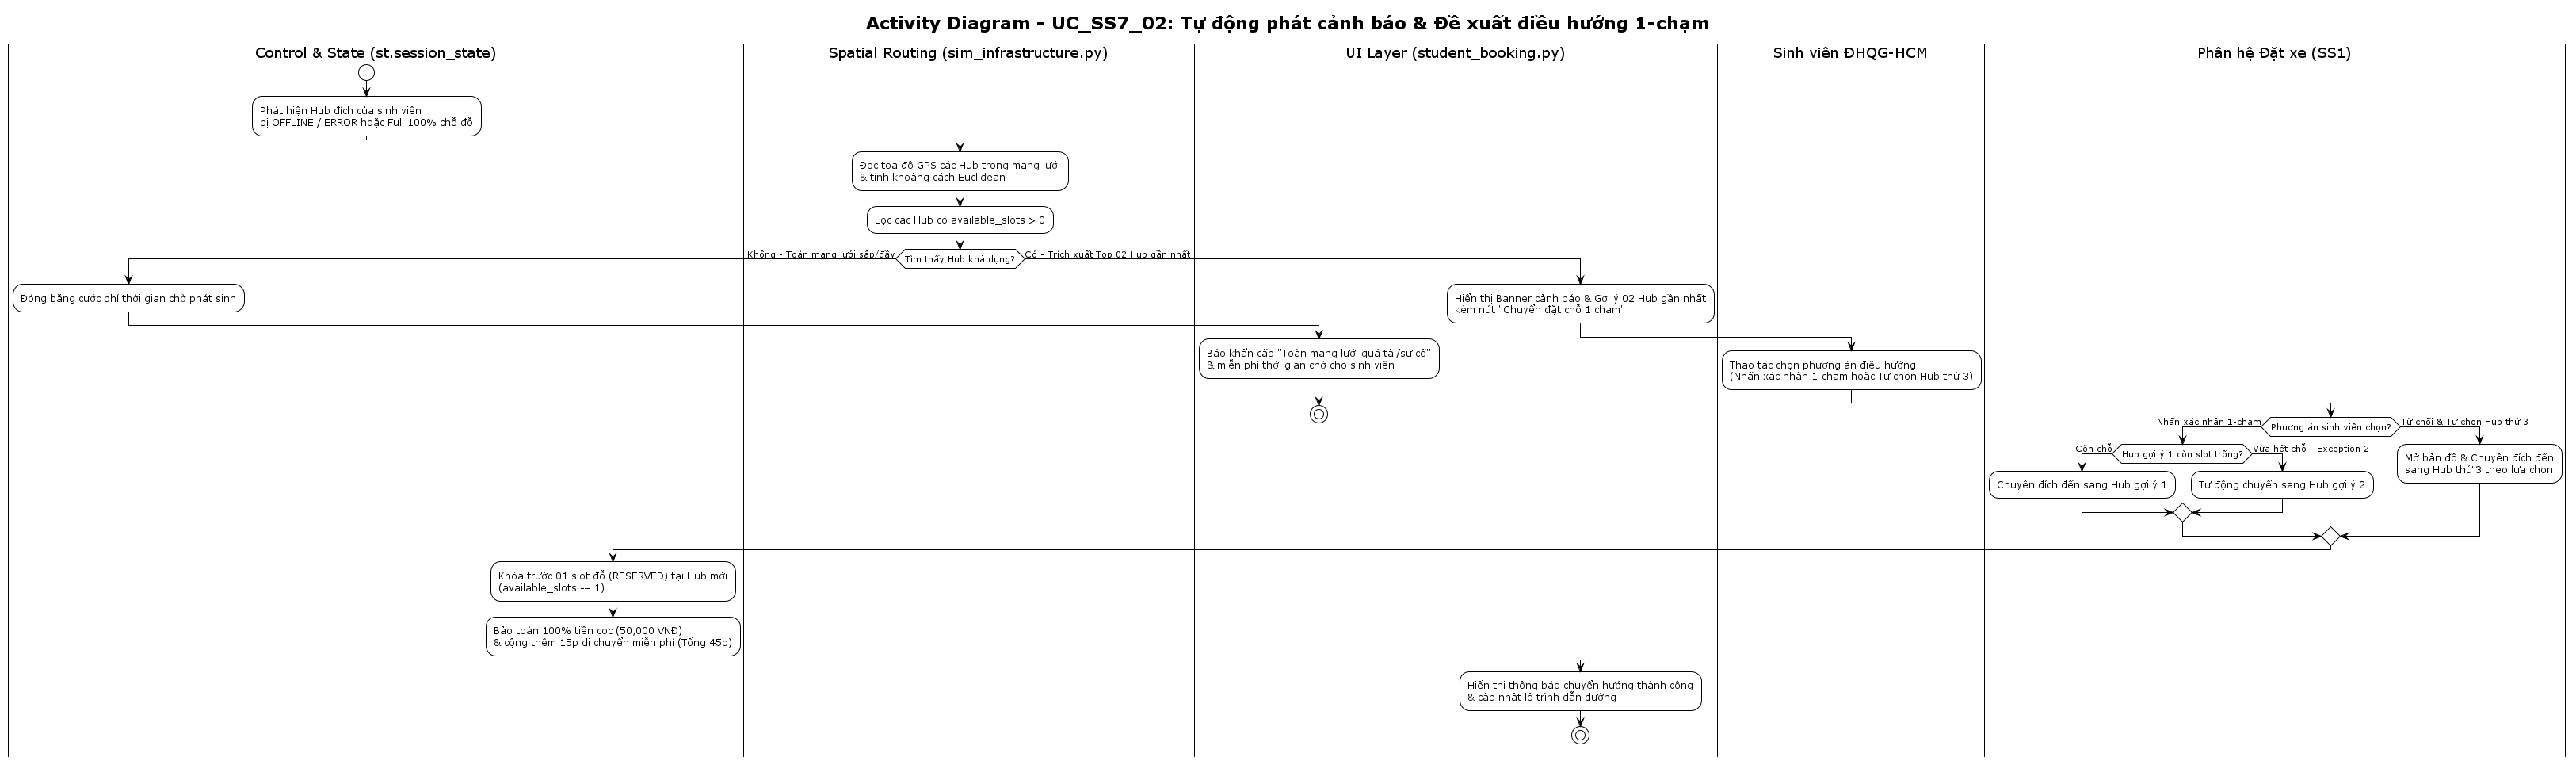
\includegraphics[width=0.98\textwidth,height=0.75\textheight,keepaspectratio]{Use-case detail-scenario/SS7/Activity diagrams/UC_SS7_02_NguyenTrungNguyen_activity.png}
    \caption{Sơ đồ Hoạt động Phân làn -- UC\_SS7\_02}
    \label{fig:act-ss7-02}
\end{figure}
\newpage

% ============================================================
%       MỤC 4: SƠ ĐỒ TRẠNG THÁI - STATE-CHART DIAGRAMS (BONUS)
% ============================================================
\section[Sơ đồ Trạng thái -- State-chart Diagrams]{Sơ đồ Trạng thái -- State-chart Diagrams\\(Bonus Work)}

\subsection{Vòng đời trạng thái Phương tiện \& Đặt chỗ}
Đặc tả vòng đời chuyển đổi trạng thái của phương tiện dùng chung từ khi sẵn sàng, được đặt chỗ, đang lưu thông, cho đến khi trả xe hoặc gặp sự cố:
\begin{center}
\small\textbf{Chuỗi chuyển trạng thái xe:} \texttt{AVAILABLE} $\xrightarrow{\text{Đặt xe}}$ \texttt{RESERVED} $\xrightarrow{\text{Mở khóa}}$ \texttt{IN\_USE} $\xrightarrow{\text{Trả xe}}$ \path{AVAILABLE / CHARGING}
\end{center}

\begin{figure}[H]
    \centering
    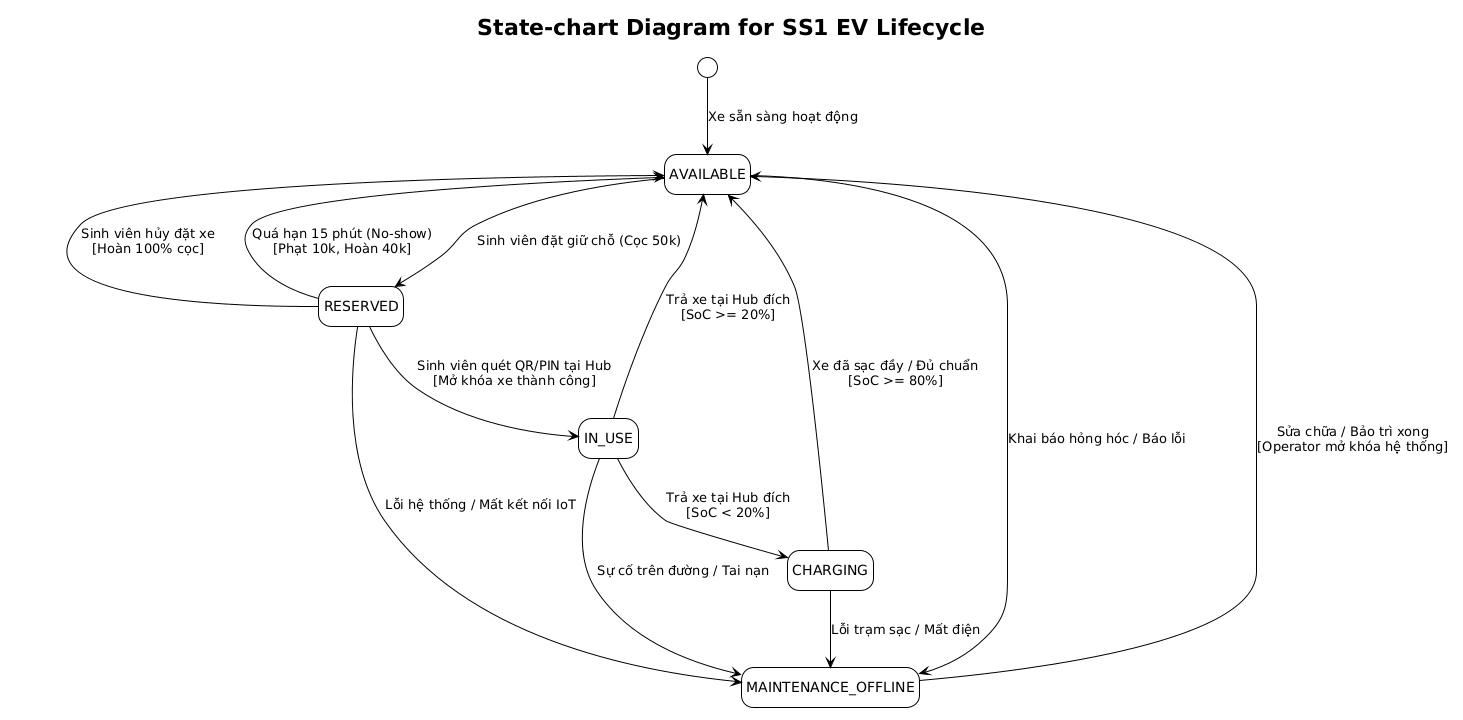
\includegraphics[width=0.92\textwidth,height=0.65\textheight,keepaspectratio]{Use-case detail-scenario/SS1/State-chart diagrams/UC_SS1_NguyenThanhDat_statechart.png}
    \caption{Sơ đồ Trạng thái Vòng đời Phương tiện Điện dùng chung (EV Lifecycle)}
    \label{fig:state-ev}
\end{figure}

\begin{table}[H]
    \centering
    \small
    \renewcommand{\arraystretch}{1.3}
    \caption{Bảng Đặc tả Chuyển Trạng thái Vòng đời Xe Điện}
    \label{tab:state-ev-spec}
    \footnotesize
    \begin{tabularx}{\textwidth}{|>{\raggedright\arraybackslash}p{2.4cm}|>{\raggedright\arraybackslash}p{2.2cm}|>{\raggedright\arraybackslash}p{2.6cm}|>{\raggedright\arraybackslash}X|>{\raggedright\arraybackslash}p{2.4cm}|}
        \hline
        \textbf{Trạng thái gốc} & \textbf{Sự kiện (Event)} & \textbf{Điều kiện (Guard)} & \textbf{Hành động (Action)} & \textbf{Trạng thái đích} \\
        \hline
        AVAILABLE & Sinh viên đặt chỗ & Số dư ví $\ge 50.000$đ & Khóa cọc, sinh mã QR/PIN & RESERVED \\
        RESERVED & Quét mã QR/PIN & Mã hợp lệ, $< 15$ phút & Mở chốt điện, tính giờ & IN\_USE \\
        RESERVED & Sinh viên hủy & Trong hạn 15 phút & Hủy đặt, hoàn 100\% cọc (50k) & AVAILABLE \\
        RESERVED & Timeout hủy (No-show) & Quá 15 phút chưa nhận & Tự hủy, phạt 10k, hoàn 40k cọc & AVAILABLE \\
        IN\_USE & Cắm trả tại Hub & Cổng khóa nhận diện, $\text{SoC} \ge 20\%$ & Tính cước, hoàn cọc thừa & AVAILABLE \\
        IN\_USE & Pin yếu & Cắm trả tại Hub, $\text{SoC} < 20\%$ & Chuyển sang hàng đợi sạc & CHARGING \\
        CHARGING & Sạc hoàn tất & Pin $\text{SoC} \ge 80\%$ (đủ chuẩn) & Rút sạc, chuyển xe khả dụng & AVAILABLE \\
        AVAILABLE & Lệnh điều phối (SS4) & Hub quá tải / Cần cân bằng & Khóa xe điều chuyển sang Hub đích & DISPATCHED \\
        DISPATCHED & Đến Hub tiếp nhận & KTV/Lái xe bàn giao tại Hub đích & Mở khóa xe, đưa vào danh sách đỗ & AVAILABLE \\
        Bất kỳ (AVAILABLE, IN\_USE, RESERVED, CHARGING) & Phát hiện sự cố (SS4) & KTV/SV báo cáo hỏng hóc, chập điện & Khóa phương tiện, ẩn khỏi app SV & INCIDENT \\
        INCIDENT & Sửa chữa tại chỗ & Lỗi nhẹ xử lý xong tại Hub & KTV nghiệm thu, mở khóa & AVAILABLE \\
        INCIDENT & Lỗi nghiêm trọng & Hỏng hóc nặng cần kéo về xưởng & Chuyển xe vào diện đại tu & {\scriptsize MAINTENANCE\_\allowbreak OFFLINE} \\
        {\scriptsize MAINTENANCE\_\allowbreak OFFLINE} & Hoàn tất đại tu & Thay thế linh kiện, kiểm định đạt & Bàn giao xe trở lại hệ thống & AVAILABLE \\
        \hline
    \end{tabularx}
\end{table}

\subsection{Vòng đời trạng thái Phiên sạc \& Cổng sạc (Phí chiếm dụng Overstay)}
Phân hệ SS5 quản lý toàn diện vòng đời sạc từ khi phương tiện vào hàng đợi, được lập lịch, cấp nguồn sạc, ân hạn rút xe và áp dụng phí chiếm dụng cổng (Overstay Fee):
\begin{center}
\small\textbf{Chuỗi chuyển trạng thái sạc:} \texttt{WAITING} $\rightarrow$ \texttt{SCHEDULED} $\rightarrow$ \texttt{CHARGING} $\rightarrow$ \texttt{CHARGE\_COMPLETED} $\rightarrow$ \texttt{GRACE\_PERIOD} $\xrightarrow{> 15\text{p}}$ \texttt{OVERSTAY} $\rightarrow$ \texttt{AVAILABLE}
\end{center}

\begin{figure}[H]
    \centering
    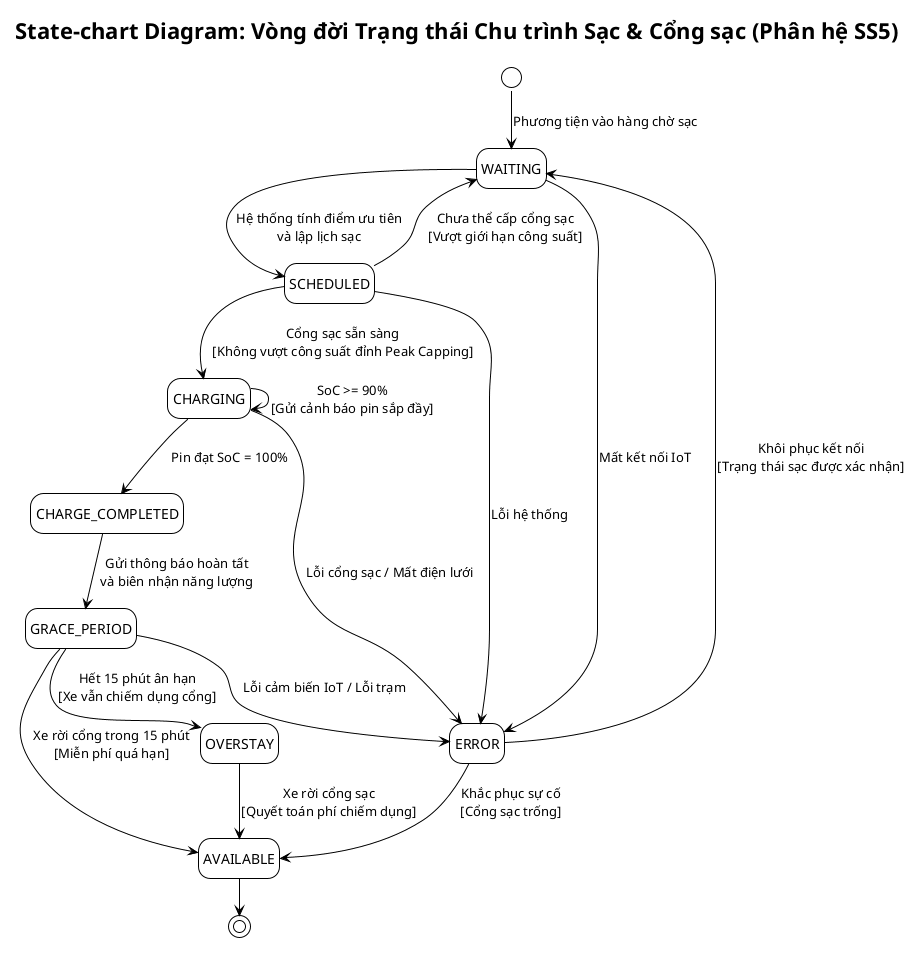
\includegraphics[width=0.92\textwidth,height=0.65\textheight,keepaspectratio]{Use-case detail-scenario/SS5/State-chart diagrams/UC_SS5_DuongDangKhoa_statechart.png}
    \caption{Sơ đồ Trạng thái Cổng sạc \& Phí chiếm dụng trụ sạc (Overstay Fee)}
    \label{fig:state-charging}
\end{figure}

\begin{table}[H]
    \centering
    \small
    \renewcommand{\arraystretch}{1.3}
    \caption{Bảng Đặc tả Chuyển Trạng thái Chu trình Sạc \& Quản lý Cổng Sạc}
    \label{tab:state-charger-spec}
    \footnotesize
    \begin{tabularx}{\textwidth}{|>{\raggedright\arraybackslash}p{2.4cm}|>{\raggedright\arraybackslash}p{2.2cm}|>{\raggedright\arraybackslash}p{2.6cm}|>{\raggedright\arraybackslash}X|>{\raggedright\arraybackslash}p{2.4cm}|}
        \hline
        \textbf{Trạng thái gốc} & \textbf{Sự kiện (Event)} & \textbf{Điều kiện (Guard)} & \textbf{Hành động (Action)} & \textbf{Trạng thái đích} \\
        \hline
        [*] & Xe cắm sạc & Xe vào hàng chờ sạc & Ghi nhận yêu cầu sạc & WAITING \\
        WAITING & Lập lịch tự động & Tính điểm ưu tiên & Sắp xếp vị trí trong hàng đợi & SCHEDULED \\
        SCHEDULED & Cấp nguồn sạc & Cổng sạc trống, không vượt công suất đỉnh & Đóng rơ-le, cấp điện áp & CHARGING \\
        SCHEDULED & Nghẽn công suất & Vượt trần tải lưới (Peak Capping) & Tạm lùi xe về hàng đợi & WAITING \\
        CHARGING & Pin đầy & $\text{SoC} = 100\%$ & Ngắt dòng sạc, xuất biên nhận & CHARGE\_\allowbreak COMPLETED \\
        CHARGE\_\allowbreak COMPLETED & Kích hoạt ân hạn & Hệ thống gửi thông báo cho SV & Khởi động đếm ngược 15 phút & GRACE\_\allowbreak PERIOD \\
        GRACE\_\allowbreak PERIOD & Rút xe đúng hạn & Rút chốt trong vòng 15 phút & Xác nhận hoàn tất, miễn phạt & AVAILABLE \\
        GRACE\_\allowbreak PERIOD & Hết giờ ân hạn & Quá 15 phút xe chưa rời cổng & Áp phí chiếm dụng 10.000đ/15p & OVERSTAY \\
        OVERSTAY & Rút xe quá hạn & Xe rời cổng sau khi phạt & Quyết toán phí quá hạn & AVAILABLE \\
        Bất kỳ (WAITING, SCHEDULED, CHARGING, GRACE) & Mất kết nối / Sự cố trạm & Cảm biến ngắt kết nối / quá nhiệt & Báo động kỹ thuật, cách ly cổng & ERROR \\
        ERROR & Khắc phục sự cố & IoT kết nối lại / Đã sửa chữa & Khôi phục về hàng đợi hoặc sẵn sàng & WAITING / AVAILABLE \\
        \hline
    \end{tabularx}
\end{table}

\subsection{Vòng đời trạng thái Vận hành của Mobility Hub}
Hệ thống giám sát Hub liên tục đánh giá tỷ lệ lấp đầy xe và trạng thái hạ tầng điện:

\begin{figure}[H]
    \centering
    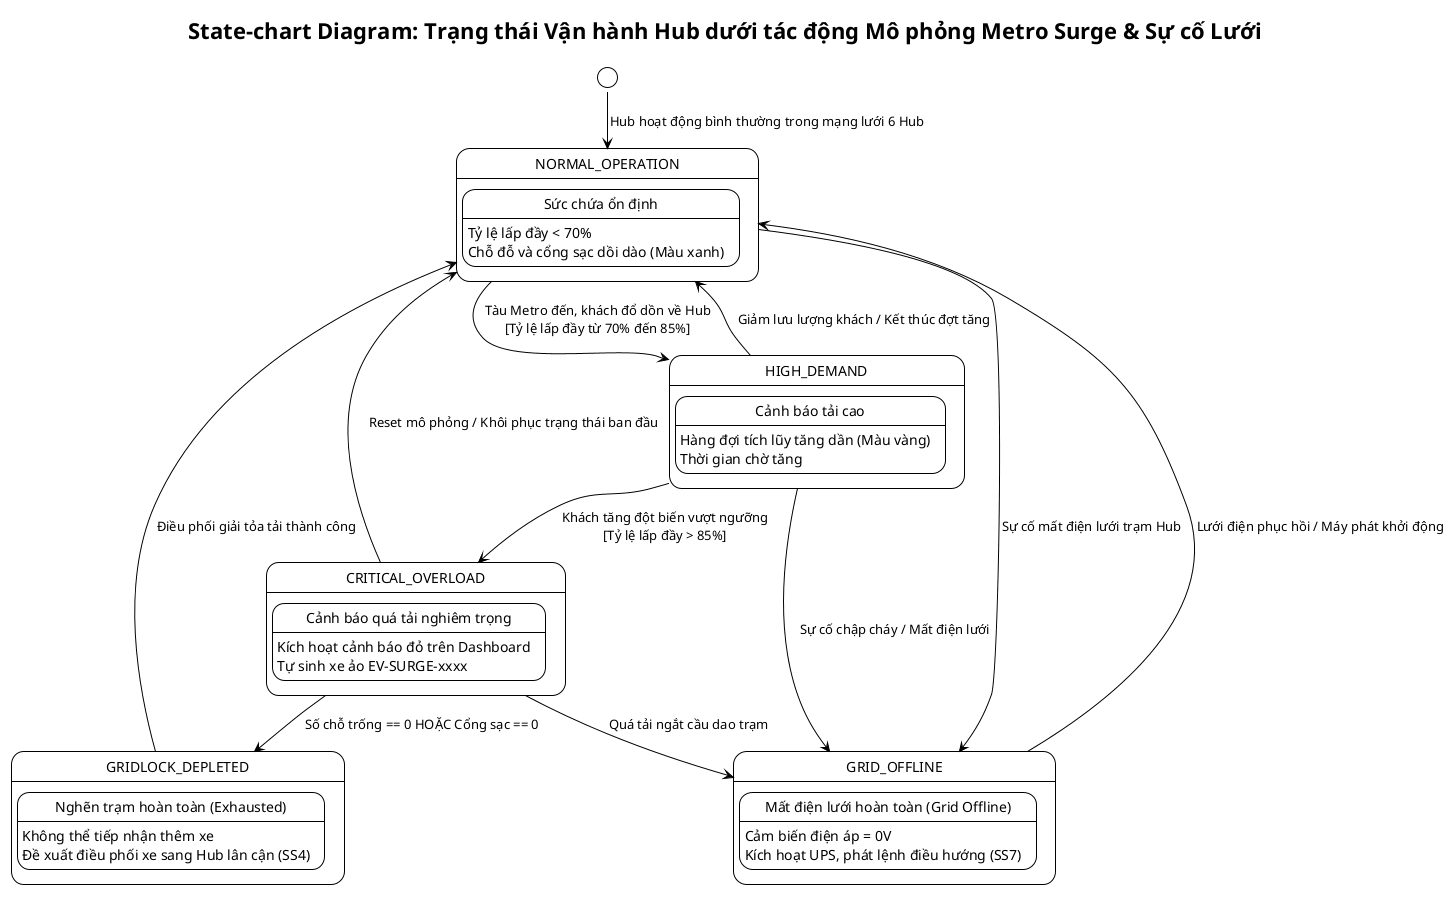
\includegraphics[width=0.92\textwidth,height=0.65\textheight,keepaspectratio]{Use-case detail-scenario/SS6/State-chart diagrams/UC_SS6_Hub_Operational_statechart.png}
    \caption{Sơ đồ Trạng thái Vận hành Mạng lưới Mobility Hub (Metro Surge)}
    \label{fig:state-hub}
\end{figure}

\begin{table}[H]
    \centering
    \small
    \renewcommand{\arraystretch}{1.3}
    \caption{Bảng Đặc tả Chuyển Trạng thái Vận hành Mạng lưới Mobility Hub}
    \label{tab:state-hub-spec}
    \footnotesize
    \begin{tabularx}{\textwidth}{|>{\raggedright\arraybackslash}p{2.6cm}|>{\raggedright\arraybackslash}p{2.2cm}|>{\raggedright\arraybackslash}p{2.6cm}|>{\raggedright\arraybackslash}X|>{\raggedright\arraybackslash}p{2.6cm}|}
        \hline
        \textbf{Trạng thái gốc} & \textbf{Sự kiện (Event)} & \textbf{Điều kiện (Guard)} & \textbf{Hành động (Action)} & \textbf{Trạng thái đích} \\
        \hline
        NORMAL\_\allowbreak OPERATION & Metro đến / Khách tăng & $70\% \le \text{Lấp đầy} \le 85\%$ & Hiển thị cảnh báo Vàng trên bản đồ & HIGH\_DEMAND \\
        HIGH\_DEMAND & Khách dồn dập vượt tải & $\text{Lấp đầy} > 85\%$ & Kích hoạt cảnh báo Đỏ, đề xuất điều xe SS4 & CRITICAL\_\allowbreak OVERLOAD \\
        HIGH\_DEMAND & Giảm lưu lượng & $\text{Lấp đầy} < 70\%$ & Trở về trạng thái bình thường (xanh) & NORMAL\_\allowbreak OPERATION \\
        CRITICAL\_\allowbreak OVERLOAD & Hết sạch chỗ đỗ / cổng & Chỗ trống $= 0$ hoặc Cổng $= 0$ & Khóa nhận xe tại Hub, cảnh báo nghẽn trạm & GRIDLOCK\_\allowbreak DEPLETED \\
        CRITICAL\_\allowbreak OVERLOAD & Hạ tải / Reset & $\text{Lấp đầy} \le 85\%$ & Khôi phục trạng thái vận hành & NORMAL\_\allowbreak OPERATION \\
        GRIDLOCK\_\allowbreak DEPLETED & Điều phối xe thành công & Giải tỏa chỗ trống $> 0$ & Mở lại luồng nhận xe & NORMAL\_\allowbreak OPERATION \\
        Bất kỳ (NORMAL, HIGH, CRITICAL) & Mất điện lưới / Chập trạm & Cảm biến điện áp $= 0\text{V}$ & Kích hoạt UPS, phát lệnh điều hướng SS7 & GRID\_\allowbreak OFFLINE \\
        GRID\_\allowbreak OFFLINE & Điện phục hồi & Điện áp ổn định $\ge 1$ phút & Đồng bộ dữ liệu IoT, mở lại trạm & NORMAL\_\allowbreak OPERATION \\
        \hline
    \end{tabularx}
\end{table}
\newpage

% ============================================================
%                       PHỤ LỤC (APPENDIX)
% ============================================================
\appendix
\section{Cấu trúc Thư mục và Mã nguồn Dự án}

\subsection{Mã nguồn Dự án (GitHub Repository)}
Mã nguồn toàn bộ hệ thống Smart E-Mobility Hub được quản lý tập trung và kiểm soát phiên bản theo chuẩn GitHub Flow tại địa chỉ chính thức:
\begin{center}
    \url{https://github.com/Dat-nguyen195/BTL_1_CNPM}
\end{center}

\subsection{Cấu trúc Thư mục Dự án (Project Structure)}
Dưới đây là cây thư mục hoàn chỉnh của dự án tại mốc bàn giao \textbf{Submission \#2}, phản ánh đầy đủ việc tổ chức các sơ đồ tuần tự, hoạt động, trạng thái và giao diện người dùng:

{\scriptsize
\begin{verbatim}
smart-emobility-hub/
|-- .gitignore                     # Cấu hình bỏ qua file biên dịch, IDE
|-- README.md                      # Tài liệu tổng quan kiến trúc và hướng dẫn cài đặt
|-- requirements.txt               # Danh mục thư viện Python (Streamlit, Plotly, ...)
|-- docs/                          # Toàn bộ tài liệu kỹ thuật của dự án
|   |-- ai-statement.md            # Cam kết liêm chính học thuật và minh bạch AI
|   |-- tasks-assignment.md        # Ma trận phân công nhiệm vụ 7 thành viên
|   |-- meeting-minutes/           # Biên bản họp nhóm định kỳ (LaTeX, Markdown, PDF)
|   |-- prompt-history/            # Lịch sử câu lệnh Prompt AI của 7 thành viên
|   |-- diagrams/                  # Toàn bộ sơ đồ thiết kế hệ thống
|   |   |-- system/                # Sơ đồ Use-Case tổng thể (smartEhub.drawio)
|   |   +-- Use-case detail-scenario/
|   |       |-- SS1/               # Phân hệ SS1 (Nguyễn Thành Đạt)
|   |       |   |-- Activity diagrams/     # UC_SS1_01..03 (.puml + .png)
|   |       |   |-- Sequence diagrams/     # UC_SS1_01..03 (.puml + .png)
|   |       |   |-- State-chart diagrams/  # EV Lifecycle (.puml + .png)
|   |       |   +-- Usecase scenario/      # Kịch bản chi tiết (.md + .docx)
|   |       |-- SS2/               # Phân hệ SS2 (Nguyễn Anh Tài)
|   |       |   |-- Activity diagrams/     # UC_SS2_01..04 (.puml + .png)
|   |       |   |-- Sequence diagrams/     # UC_SS2_01..04 (.puml + .png)
|   |       |   |-- State-chart diagrams/  # Personal EV (.puml + .png)
|   |       |   +-- Usecase scenario/      # Kịch bản chi tiết (.md + .docx)
|   |       |-- SS3/               # Phân hệ SS3 (Phạm Tiến Đạt)
|   |       |   |-- Activity diagrams/     # UC_SS3_01..02 (.puml + .png)
|   |       |   |-- Sequence diagrams/     # UC_SS3_01..02 (.puml + .png)
|   |       |   |-- State-chart diagrams/  # Hub Monitoring (.puml + .png)
|   |       |   +-- Usecase scenario/      # Kịch bản chi tiết (.md + .docx)
|   |       |-- SS4/               # Phân hệ SS4 (Đặng Hoàng Quý Nhân)
|   |       |   |-- Activity diagrams/     # UC_SS4_01..02 (.puml + .png)
|   |       |   |-- Sequence diagrams/     # UC_SS4_01..02 (.puml + .png)
|   |       |   |-- State-chart diagrams/  # Dispatch & Incident (.puml + .png)
|   |       |   +-- Usecase scenario/      # Kịch bản chi tiết (.md + .docx)
|   |       |-- SS5/               # Phân hệ SS5 (Dương Đăng Khoa)
|   |       |   |-- Activity diagrams/     # UC_SS5_01..02 (.puml + .png)
|   |       |   |-- Sequence diagrams/     # UC_SS5_01..02 (.puml + .png)
|   |       |   |-- State-chart diagrams/  # Charging Lifecycle (.puml + .png)
|   |       |   +-- Usecase scenario/      # Kịch bản chi tiết (.md + .docx)
|   |       |-- SS6/               # Phân hệ SS6 (Hoàng Văn Tấn)
|   |       |   |-- Activity diagrams/     # UC_SS6_01..02 (.puml + .png)
|   |       |   |-- Sequence diagrams/     # UC_SS6_01..02 (.puml + .png)
|   |       |   |-- State-chart diagrams/  # Metro Surge (.puml + .png)
|   |       |   +-- Usecase scenario/      # Kịch bản chi tiết (.md + .docx)
|   |       +-- SS7/               # Phân hệ SS7 (Nguyễn Trung Nguyên)
|   |           |-- Activity diagrams/     # UC_SS7_01..02 (.puml + .png)
|   |           |-- Sequence diagrams/     # UC_SS7_01..02 (.puml + .png)
|   |           |-- State-chart diagrams/  # Infrastructure (.puml + .png)
|   |           +-- Usecase scenario/      # Kịch bản chi tiết (.md + .docx)
|   +-- report/                    # Báo cáo các đợt nộp học phần CO3001
|       |-- assets/                # Logo ĐHBK và hình ảnh bìa mẫu dùng chung
|       |   +-- mau.png
|       |-- scripts/               # Scripts tự động sinh báo cáo
|       |-- submission_1/          # Báo cáo Submission #1 (Đặc tả Yêu cầu)
|       |   |-- REPORT_SUBMISSION_1.tex
|       |   +-- REPORT_SUBMISSION_1.pdf
|       +-- submission_2/          # Báo cáo Submission #2 (Thiết kế Kiến trúc & UML)
|           |-- REPORT_SUBMISSION_2.tex # File mã nguồn LaTeX chính
|           +-- REPORT_SUBMISSION_2.pdf
+-- src/                           # Mã nguồn Prototype hệ thống (Streamlit)
    |-- app.py                     # Entry point khởi chạy ứng dụng
    |-- components/                # UI components tương ứng 7 phân hệ
    |-- core/                      # Thuật toán điều phối, lập lịch và mô phỏng
    +-- data/                      # Dữ liệu mô phỏng mạng lưới Hub
\end{verbatim}
}

\section{Tuyên bố Minh bạch Sử dụng Trí tuệ Nhân tạo (Generative AI Disclosure Statement)}
\label{sec:ai-statement}

Căn cứ quy định về Liêm chính Học thuật của Trường Đại học Bách Khoa -- ĐHQG-HCM và đề cương học phần Công nghệ Phần mềm (CO3001), tập thể nhóm BEE BRAVE công khai và minh bạch 100\% việc sử dụng các công cụ Trí tuệ Nhân tạo Tạo sinh (Generative AI) trong quá trình thực hiện giai đoạn \textbf{Submission \#2}:

\subsection{Nguyên tắc Cốt lõi}
\begin{itemize}[nosep]
    \item \textbf{Minh bạch Tuyệt đối (Full Transparency):} Mọi công cụ AI hỗ trợ (Claude, ChatGPT, Gemini) đều được khai báo cụ thể theo từng thành viên và từng phân hệ phụ trách.
    \item \textbf{AI là Trợ lý Kỹ thuật (Technical Assistant):} Công cụ AI chỉ đóng vai trò hỗ trợ kiểm tra cú pháp LaTeX/PlantUML, gợi ý boilerplate giao diện Streamlit, và rà soát lỗi chính tả bảng biểu; tuyệt đối không thay thế tư duy phân tích nghiệp vụ, mô hình hóa kiến trúc và quyết định kỹ thuật của sinh viên.
    \item \textbf{Trách nhiệm Cá nhân (Individual Accountability):} Mỗi thành viên chịu trách nhiệm giải trình toàn diện về logic nghiệp vụ, tính đúng đắn của sơ đồ UML và mã nguồn thực thi thuộc phân hệ của mình khi bảo vệ trước Hội đồng chấm thi.
\end{itemize}

\subsection{Quy trình Xác minh của Con người (Human Verification)}
Nhóm sử dụng quy trình xác minh 3 bước dưới đây; kết quả tự động không xác nhận thay phần rà soát của từng thành viên:
\begin{enumerate}[nosep]
    \item \textbf{Bước 1 -- Tự kiểm tra độc lập (Self-check):} Thành viên tự kiểm tra tính nhất quán giữa kịch bản nghiệp vụ Use-case và sơ đồ PlantUML (Sequence, Activity, State-chart).
    \item \textbf{Bước 2 -- Rà soát chéo (Peer Review):} Thực hiện kiểm thử chéo luồng dữ liệu và biên tập tài liệu theo phân công trong biên bản họp nhóm.
    \item \textbf{Bước 3 -- Tổng duyệt Tích hợp (System Audit):} Nhóm trưởng xác thực việc biên dịch 0 lỗi XeLaTeX, chạy toàn bộ bộ kiểm thử tự động (\texttt{pytest}) và đối chiếu bằng chứng ảnh chụp giao diện thực tế.
\end{enumerate}

Nhật ký câu lệnh Prompt chi tiết của 7 thành viên được lưu vết đầy đủ tại thư mục: \path{docs/prompt-history/}.

\end{document}
